% !TEX TS-program = pdflatex
% !TEX encoding = UTF-8 Unicode

% This is a simple template for a LaTeX document using the "article" class.
% See "book", "report", "letter" for other types of document.

\documentclass[12pt]{article} % use larger type; default would be 10pt

\RequirePackage[colorlinks,citecolor=blue,urlcolor=blue]{hyperref}
\usepackage[utf8]{inputenc} % set input encoding (not needed with XeLaTeX)

%%% Examples of Article customizations
% These packages are optional, depending whether you want the features they provide.
% See the LaTeX Companion or other references for full information.

%%% PAGE DIMENSIONS
\usepackage{geometry} % to change the page dimensions
\geometry{letterpaper} % or letterpaper (US) or a5paper or....
\geometry{margin=1in} % for example, change the margins to 2 inches all round
% \geometry{landscape} % set up the page for landscape
%   read geometry.pdf for detailed page layout information

\usepackage{graphicx} % support the \includegraphics command and options
%\usepackage{setspace}

% \usepackage[parfill]{parskip} % Activate to begin paragraphs with an empty line rather than an indent

%%% PACKAGES
\usepackage{booktabs} % for much better looking tables
\usepackage{array} % for better arrays (eg matrices) in maths
\usepackage{paralist} % very flexible & customisable lists (eg. enumerate/itemize, etc.)
\usepackage{verbatim} % adds environment for commenting out blocks of text & for better verbatim
\usepackage{subfig} % make it possible to include more than one captioned figure/table in a single float
\usepackage{amsbsy}
\usepackage{amsmath}
\usepackage{amssymb}
\usepackage{amsfonts}
\usepackage{amscd}
\usepackage{amsthm}
\usepackage{mathabx}
\usepackage{cite}
\usepackage{dutchcal}
\usepackage{float}
\usepackage[toc,page]{appendix}
%\usepackage{natbib}
%\usepackage{lineno}
\usepackage{mathrsfs}
%\usepackage[nolists]{endfloat}
\usepackage{todonotes}
\usepackage{setspace}
\usepackage{multirow}
\usepackage{algorithm}
\usepackage{algorithmicx}
\usepackage{algpseudocode}
\usepackage{listings}
\usepackage{parskip}
%\usepackage{mathptmx}
%\DeclareMathAlphabet{\mathcal}{OMS}{cmsy}{m}{n}
% These packages are all incorporated in the memoir class to one degree or another...

%%% HEADERS & FOOTERS
\usepackage{fancyhdr} % This should be set AFTER setting up the page geometry
\pagestyle{fancy} % options: empty , plain , fancy
\renewcommand{\headrulewidth}{0pt} % customise the layout...
\lhead{}\chead{}\rhead{}
\lfoot{}\cfoot{\thepage}\rfoot{}

%%% SECTION TITLE APPEARANCE
\usepackage{sectsty}
\allsectionsfont{\sffamily\mdseries\upshape} % (See the fntguide.pdf for font help)
% (This matches ConTeXt defaults)

%%% ToC (table of contents) APPEARANCE
\usepackage[nottoc,notlof,notlot]{tocbibind} % Put the bibliography in the ToC
\usepackage[titles,subfigure]{tocloft} % Alter the style of the Table of Contents
\renewcommand{\cftsecfont}{\rmfamily\mdseries\upshape}
\renewcommand{\cftsecpagefont}{\rmfamily\mdseries\upshape} % No bold!

%%% END Article customizations

%%% The "real" document content comes below...
%Variable Declarations
%Matricies
%\graphicspath{{Figures/}}

\def\diffvar{\boldsymbol{\Sigma}}

\newcommand{\vecEpsilon}[0]{\boldsymbol{\epsilon}}
\newcommand{\Expected}[1]{{\mathbf{E}\left(#1\right)}}
\newcommand{\Var}[1]{\mathbf{Var}\left(#1\right)}
\newcommand{\vecc}[1]{\mathbf{#1}}
\newcommand{\p}[1]{{\mathbf{p}}_{#1}}
\newcommand{\q}[1]{{\mathbf{q}}_{#1}}
\newcommand{\M}[1]{{\mathbf{M}}_{#1}}
\newcommand{\Q}[1]{{\mathbf{Q}}_{#1}}
\newcommand{\Smat}[1]{{\mathbf{S}}_{#1}}
\newcommand{\X}[1]{{\mathbf{X}_{#1}}}
\newcommand{\D}[1]{{\mathbf{D}_{#1}}}
\newcommand{\V}[1]{{\mathbf{V}_{#1}}}
\newcommand{\G}[1]{{\mathbf{G}_{#1}}}
\newcommand{\bl}[1]{{b}_{#1}} % for branch length
\newcommand{\br}[1]{{r}_{#1}} % for branch rate
\newcommand{\bp}[1]{{\nu}_{#1}} % for branch parameter
\newcommand{\sr}[1]{{\gamma}_{#1}} % for site rate
\newcommand{\Ptr}[1]{\mathbf{P}_{#1}}

\newcommand{\cDensity}[2]{\ensuremath{P(#1 \,|\,#2)}}
\newcommand{\veccDensity}[2]{\mathbf{p}(#1 \,|\,#2)}
\newcommand{\matcDensity}[2]{\mathbf{P}(#1 \,|\,#2)}
\newcommand{\secondDerivative}[3]{\frac{\partial ^2}{\partial #1 _i\partial #2 _j}{#3}}
\newcommand{\density}[1]{\ensuremath{p(#1 )}}
\newcommand{\vecOperator}[1]{\mbox{vec}\hspace{-0.1em}\left[ #1 \right]}
\newcommand{\trOperator}[1]{\mbox{tr}\hspace{-0.1em}\left[ #1 \right]}
\newcommand{\oneVector}[1]{\mathbf{1}_{#1}}
\newcommand{\order}[1]{{\cal O}\hspace{-0.1em}\left( #1 \right)}
\newcommand{\specialInverse}{-}
\newcommand{\inverse}{^{-1}}
\newcommand{\transpose}{^T}
\newcommand{\vectorize}[1]{\text{vec}\left(#1\right)}
\newcommand{\kronecker}{\otimes}

\newcommand{\parent}[1]{\text{pa}(#1)}
\newcommand{\parentNth}[2]{\text{pa}^{(#2)}(#1)}
\newcommand{\sibling}[1]{\text{sib}(#1)}
\newcommand{\smallParent}[1]{\text{\tiny pa}(#1)}
\newcommand{\nodePrecision}[1]{\mathbf{P}_{#1}}
\newcommand{\nodeVariance}[1]{\mathbf{\Sigma}_{#1}}
\newcommand{\nodeVarianceFunction}[1]{\nodeVariance{}\hspace{-0.1em}\left( #1 \right)}
\newcommand{\deflatedNodePrecision}[1]{\nodePrecision{#1}^{\star}}
\newcommand{\nodeMean}[1]{\mathbf{m}_{#1}}
\newcommand{\nodeIndexOne}{i}
\newcommand{\nodeIndexTwo}{j}
\newcommand{\nodeIndexThree}{k}
\newcommand{\branchLength}[1]{t_{#1}}
\newcommand{\diffusionVariance}{\diffvar}
\newcommand{\remainder}[1]{r_{#1}}
\newcommand{\backback}{-0.15em}
\newcommand{\zeroDimension}[1]{d\hspace{\backback}\left(#1\right)}
\newcommand{\infiniteDimension}[1]{e\hspace{\backback}\left(#1\right)}
\newcommand{\finiteNonZeroDimension}[1]{f\hspace{\backback}\left(#1\right)}
\newcommand{\permutationMatrix}{\mathbf{Q}}
\newcommand{\nodePermutationMatrix}[1]{\permutationMatrix_{#1}}
%\newcommand{\transpose}{^{'}}
\newcommand{\missing}[2]{\delta_{#1 #2}}
\newcommand{\traitIndex}{p}
\newcommand{\arbitraryMatrix}{\mathbf{Z}}
\newcommand{\identityMatrix}[1]{\mathbf{I}_{#1}}
\newcommand{\bigzero}[2]{\makebox(0,0){\hspace{#1}\vspace{#2}\text{\huge0}}}
\newcommand{\altDet}[1]{\hat{\text{det}}\left( #1 \right)}
\newcommand{\changeDimension}[1]{\Delta_{#1}}
\newcommand{\notMissingMatrix}[1]{\boldsymbol{\delta}_{#1}}

\newcommand{\nodePreMean}[1]{\mathbf{n}_{#1}}
\newcommand{\nodePreVariance}[1]{\mathbf{W}_{#1}}
\newcommand{\nodePrePrecision}[1]{\mathbf{Q}_{#1}}
\newcommand{\deflatedNodePrePrecision}[1]{\nodePrePrecision{#1}^{\star}}
%\newcommand{\MVN}{\text{MVN}}
\newcommand{\Indexobs}{\mathcal{I}^{\text{\tiny obs}}_ \nodeIndexOne}
\newcommand{\Indexmis}{\mathcal{I}^{\text{\tiny mis}}_ \nodeIndexOne}

\newcommand{\normalDensityFunction}[3]{{\cal N}\hspace{-0.25em}\left( #1; #2, #3 \right)}
\newcommand{\conditionalMean}[1]{\boldsymbol{\mu}_{#1}}
\newcommand{\dd}{\text{d}}
\def\rowvarresidMissing{\rowvarresid_{{mis}_\nodeIndexOne}}

\newcommand{\symbolicObservedVariance}{0}
\newcommand{\symbolicMissingVariance}{\infty}
\newcommand{\symbolicFiniteVariance}{+}
\newcommand{\partialDiffusionVariance}[2]{\diffusionVariance_{#1 #2}}

\newcommand{\observedVariance}{\partialDiffusionVariance{\symbolicObservedVariance}{\symbolicObservedVariance}}
\newcommand{\missingVariance}{\partialDiffusionVariance{\symbolicMissingVariance}{\symbolicMissingVariance}}
\newcommand{\finiteVariance}{\partialDiffusionVariance{\symbolicFiniteVariance}{\symbolicFiniteVariance}}
\newcommand{\tipLatentPrecision}[1]{\mathbf{R}_{#1}}

\newcommand{\finiteObservedVariance}{\partialDiffusionVariance{\symbolicFiniteVariance}{\symbolicObservedVariance}}
\newcommand{\finiteMissingVariance}{\partialDiffusionVariance{\symbolicFiniteVariance}{\symbolicMissingVariance}}
\newcommand{\observedMissingVariance}{\partialDiffusionVariance{\symbolicObservedVariance}{\symbolicMissingVariance}}
\newcommand{\diag}[1]{\text{diag} \left[ #1 \right]}

\newcommand{\deflatedPrecision}[1]{\mathbf{P}^{\star}_{#1}}
\newcommand{\startingPrecision}[1]{\mathbf{P}_{#1}}
\newcommand{\finitePrecision}[1]{\tilde{\startingPrecision{#1}}}
\newcommand{\bogusPrecision}[1]{\finitePrecision{#1}^{-1}}
\newcommand{\raisedInfty}{\raisebox{0.1em}{$\infty$}}
\newcommand{\bfZero}{\mathbf{0}}
\newcommand{\missingIndicator}[1]{\mathbf{M}_{#1}}

\newcommand{\phylogeny}{\mathscr{F}}
\newcommand{\phylogenyVariance}{\mathbf{\Upsilon}}
\newcommand{\phylogenyPrecision}{\phylogenyVariance\inverse}
\newcommand{\traitPrecision}{\mathbf{P}}

\newcommand{\grandVariance}{\mathbf{\Sigma}}
\newcommand{\grandVarianceExpression}{\traitPrecision\inverse \kronecker \phylogenyVariance}
\newcommand{\grandPrecision}{\grandVariance\inverse}
\newcommand{\grandPrecisionExpression}{\traitPrecision \kronecker \phylogenyPrecision}

\newcommand{\latentData}{\mathbf{Y}}
\newcommand{\vecLatentData}{\mathbf{Z}}
\newcommand{\nTaxa}{N}
\newcommand{\nTraits}{P}

\newcommand{\mvnDensity}[2]{\text{MVN}\hspace{-0.1em}\left(#1, #2\right)}
\newcommand{\mvn}[3]{\text{MVN}\hspace{-0.1em}\left(#1; #2, #3\right)}
\newcommand{\gradient}[1]{\frac{\partial}{\partial #1}}

\newcommand{\rate}[1]{\phi_{#1}}
\newcommand{\allRates}{\boldsymbol{\phi}}
\newcommand{\rank}{\mbox{rank}}
\newcommand{\sVar}{\rm Var}

\newcommand{\distas}[1]{\overset{#1}{\sim}}%

\usepackage{empheq}
\newcommand*\widefbox[1]{\fbox{\hspace{2em}#1\hspace{2em}}}

\usepackage{etoolbox,environ}
\newtoggle{showProof}
\togglefalse{showProof}
\NewEnviron{pf}
  {\iftoggle{showProof}{\BODY}{}}


\usepackage{scalerel,stackengine}
\stackMath
\newcommand\reallywidehat[1]{%
\savestack{\tmpbox}{\stretchto{%
  \scaleto{%
    \scalerel*[\widthof{\ensuremath{#1}}]{\kern-.6pt\bigwedge\kern-.6pt}%
    {\rule[-\textheight/2]{1ex}{\textheight}}%WIDTH-LIMITED BIG WEDGE
  }{\textheight}% 
}{0.5ex}}%
\stackon[1pt]{#1}{\tmpbox}%
}
\colorlet{shadecolor}{gray!15}

\DeclareMathAlphabet{\mathcal}{OMS}{cmsy}{m}{n}
\newcommand{\columnSpace}[1]{\mathnormal{C}(#1)}
\newcommand{\dimm}{\mbox{dim}}
\newcommand{\Null}[1]{\mathcal{N}(#1)}

\def\treeTraitsRoot{\boldsymbol{\mu}_R}
\def\diffprec{\boldsymbol{\Lambda}_R}
\def\diffprecprior{\boldsymbol{\Lambda}_{R_0}}
\def\diffmean{\boldsymbol{\mu}_0}
\def\pss{\kappa_0}
\def\diffprecpriordf{\nu}
\def\pss{\kappa_0}

\newtheorem{thm}{Theorem}
\newtheorem{lemma}{Lemma}
\newtheorem{prop}{Proposition}
\newtheorem{cor}{Corollary}
\newtheorem{remark}{Remark}
\newtheorem{example}{Example}
\newtheorem{mydef}{Definition}
\newtheorem{assumption}{Assumption}

\usepackage{chngcntr}
\counterwithin{figure}{section}

\DeclareMathOperator*{\argmax}{arg\,max}
\DeclareMathOperator*{\argmin}{arg\,min}

\toggletrue{showProof}
\begin{document}

\bigskip
\medskip
\begin{center}

\noindent{\Large \bf Math 6040/7260 Linear Models\\}
\noindent{Mon/Wed/Fri 10:55am - 11:40am \\
Instructor: Dr. Xiang Ji, xji4@tulane.edu}
\bigskip

\end{center}


\section{Lecture 1:Jan 20}

\subsection*{Today}
\begin{itemize}
\item Introduction
\item Course logistics
\item Read JF chapter 1, JM Appendix A
\end{itemize}

\subsection*{What is this course about?}
The term “linear models” describes a wide class of methods for the statistical analysis of multivariate data.
The underlying theory is grounded in linear algebra and multivariate statistics, but applications range from biological research to public policy.
The objective of this course is to provide a solid introduction to both the theory and practice of linear models, combining mathematical concepts with realistic examples.

\subsection*{A hierarchy of linear models}

\begin{itemize}
\item The linear mean model:
$$
\mathop \mathbf{y} \limits_{n \times 1} = \mathop \mathbf{X}\limits_{n \times p} \mathop \beta \limits_{p \times 1}+  \mathop \epsilon \limits_{n \times 1}
$$
where $\Expected{\epsilon} = \vecc{0}$.  Only assumption is that errors have mean $0$.

\item Gauss-Markov model:
$$
\mathbf{y} = \mathbf{X}\beta + \vecEpsilon
$$
where $\Expected{\vecc{\epsilon}} = \vecc{0}$ and $\Var{\vecc{\epsilon}} = \sigma^2 \vecc{I}$.  Uncorrelated errors with constant variance.

\item Aitken model or general linear model:
$$
\mathbf{y} = \mathbf{X}\beta + \vecEpsilon
$$
where $\Expected{\vecc{\epsilon}} = \vecc{0}$ and $\Var{\vecc{\epsilon}} = \sigma^2 \vecc{V}$.  $\vecc{V}$ is fixed and known.

\item Variance components models: $\vecc{y} \sim N(\vecc{X}\beta, \sigma^2_1\vecc{V}_1 + \sigma^2_2\vecc{V}_2 + \dots + \sigma^2_r\vecc{V}_r)$ with $\vecc{V}_1, \vecc{V}_2, \dots, \vecc{V}_r$ known.

\item General mixed linear Model:
$$
\mathbf{y} = \mathbf{X}\beta + \vecEpsilon
$$
where $\Expected{\vecc{\epsilon}} = \vecc{0}$ and $\Var{\vecc{\epsilon}} = \boldsymbol{\Sigma}(\theta)$.

\item Generalized linear models (GLMs).  Logistic regression, probit regression, log-linear model (Poisson regression), ... Note the difference from the general linear model.  GLMs are generalization of the {\it concept} of linear models.  They are covered in Math 7360 - Data Analysis class (\href{https://tulane-math7360.github.io/lectures/}{https://tulane-math7360.github.io/lectures/}).

\end{itemize}

\subsection*{Syllabus}

Check course website frequently for updates and announcements.

\href{https://tulane-math-7260-2021.github.io/}{https://tulane-math-7260-2021.github.io/}

\subsection*{HW submission}

Through Github with demo on Friday class.





\newpage
\setcounter{section}{1}

\section{Lecture 2:Jan 22}

\subsection*{Last time}
\begin{itemize}
\item Introduction
\item Course logistics
\end{itemize}

\subsection*{Today}
\begin{itemize}
\item Introduce yourself (remind remote students to record a short video)
  \begin{itemize}
    \item basic info (name, department, year, ...)
    \item why taking this course
  \end{itemize}
\item Git
\item Linear algebra: vector and vector space, rank of a matrix
\end{itemize}

\subsection*{What is git?}
Git is currently the most popular system for version control according to \href{https://trends.google.com/trends/explore?date=all&q=\%2Fm\%2F05vqwg,\%2Fm\%2F012ct9,\%2Fm\%2F08441_,\%2Fm\%2F08w6d6,\%2Fm\%2F09d6g&hl=en-US&tz=&tz=}{Google Trend}.\\
Git was initially designed and developed by \href{http://en.wikipedia.org/wiki/Linus_Torvalds}{Linus Torvalds} in 2005 for Linux kernel development.  Git is the British English slang for unpleasant person.

\subsection*{Why using git?}
\begin{itemize}
  \item \href{https://github.com/}{GitHub} is becoming a de facto central repository for open source development. 
  \item {\bf Advertise} yourself through GitHub (e.g., host a free personal webpage on GitHub).
  \item a skill that employers look for (according to \href{http://magazine.amstat.org/blog/2018/01/01/data-science-mooc/}{this AmStat article}).
\end{itemize}

\subsection*{Git workflow}

Figure~\ref{fig:gitflow} shows its basic workflow.
\begin{figure}[!h]
\begin{center}
  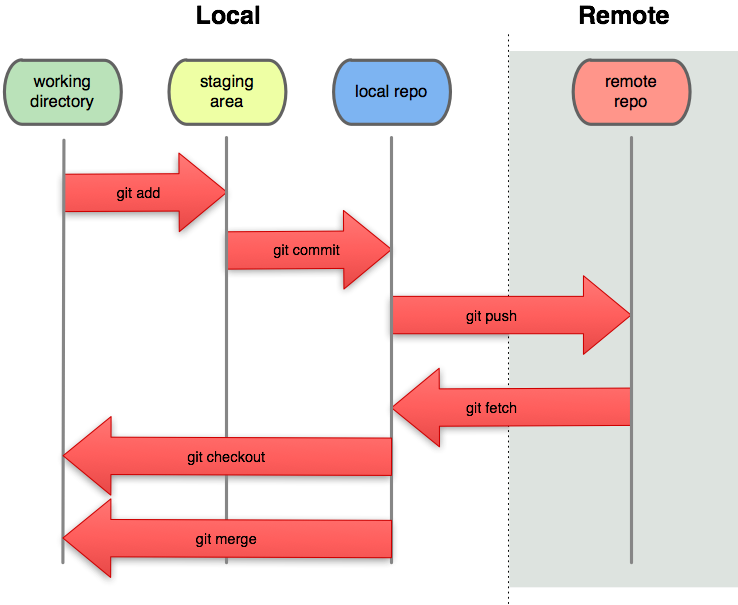
\includegraphics[width=0.8\textwidth]{Lecture2/git_workflow.png}
  \caption{}
  \label{fig:gitflow}
\end{center}
\end{figure}

\subsection*{What do I need to use Git?}

\begin{itemize}
\item A {\bf Git server} enabling multi-person collaboration through a centralized repository.
\item A {\bf Git client} on your own machine.

  \begin{itemize}
    \item Linux: Git client program is shipped with many Linux distributions, e.g., Ubuntu and CentOS. If not, install using a package manager, e.g., \colorbox{shadecolor}{yum install git} on CentOS.
    \item Mac: follow instructions at \href{https://www.atlassian.com/git/tutorials/install-git}{https://www.atlassian.com/git/tutorials/install-git}.
    \item Windows: Git for Windows at \href{https://gitforwindows.org}{https://gitforwindows.org} (GUI) aka Git Bash.
  \end{itemize}
\item Do {\bf not} totally rely on GUI or IDE. Learn to use Git on command line, which is needed for cluster and cloud computing.

\end{itemize}

\subsection*{Git survival commands}

\begin{itemize}
  \item \colorbox{shadecolor}{git pull} synchronize local Git directory with remote repository.
  \item Modify files in local working directory.
  \item \colorbox{shadecolor}{git add FILES} add snapshots to staging area
  \item \colorbox{shadecolor}{git commit -m ``message''} store snapshots permanently to ({\bf local}) Git repository
  \item \colorbox{shadecolor}{git push} push commits to remote repository.
\end{itemize}

\subsection*{Git basic usage}

Working with your local copy.

\begin{itemize}

    \item \colorbox{shadecolor}{git pull}: update local Git repository with remote repository (fetch + merge).
    
    \item \colorbox{shadecolor}{git log FILENAME}: display the current status of working directory.
    
    \item \colorbox{shadecolor}{git diff}: show differences (by default difference from the most recent commit). 
    
    \item \colorbox{shadecolor}{git add file1 file2 ...}: add file(s) to the staging area.
    
    \item \colorbox{shadecolor}{git commit}: commit changes in staging area to Git directory.
    
    \item \colorbox{shadecolor}{git push}: publish commits in local Git repository to remote repository.

    \item \colorbox{shadecolor}{git reset --soft HEAD~1}: undo the last commit. 

    \item \colorbox{shadecolor}{git checkout FILENAME}: go back to the last commit, discarding all changes made.
    
    \item \colorbox{shadecolor}{git rm FILENAME}: remove files from git control.
\end{itemize}


\newpage
\subsection*{Vector and vector space}

(from JM Appendix A)

\begin{itemize}
\item A set of vectors $\vecc{x}_1, \dots, \vecc{x}_n$ are {\it linearly dependent} if there exist coefficients $c_j$ for $j = 1, 2, \dots, n$ such that $\sum_{j=1}^{n}{c_j \vecc{x}_j} = \vecc{0}$ and $||\vecc{c}||_2 = \sum_{j=1}^{n}{c_j^2}>0$.
They are {\it linearly independent} if  $\sum_{j=1}^{n}{c_j \vecc{x}_j} = \vecc{0}$ implies $c_j = 0$ for all $j$.

\item Two vectors are {\it orthogonal} to each other, written $\vecc{x} \bot \vecc{y}$, if their inner product is 0, that is $\vecc{x}\transpose\vecc{y} = \vecc{y}\transpose\vecc{x} = \sum\limits_{j}{x_j y_j} = 0$.

\item A set of vectors $\vecc{x}^{(1)}, \vecc{x}^{(2)}, \dots, \vecc{x}^{(n)}$ are mutually orthogonal iff $\vecc{x}^{(i)T}\vecc{x}^{(j)} = 0$ for $\forall i \ne j$.

\item The most common set of vectors that are mutually orthogonal are the {\it elementary} vectors $\vecc{e}^{(1)}, \vecc{e}^{(2)}, \dots, \vecc{e}^{(n)}$, which are all zero, except for one element equal to $1$, so that $\vecc{e}^{(i)}_i = 1$ and $\vecc{e}^{(i)}_j = 0, \forall j \ne i$.

\item A {\it vector space} $\mathcal{S}$ is a set of vectors that are closed under addition and scalar multiplication, that is 

  \begin{itemize}
    \item if $\vecc{x}^{(1)}$ and $\vecc{x}^{(2)}$ are in $\mathcal{S}$, then $c_1 \vecc{x}^{(1)} + c_2 \vecc{x}^{(2)}$ is in $\mathcal{S}$.
  \end{itemize}

\item A vector space $\mathcal{S}$ is {\it generated} or {\it spanned} by a set of vectors $\vecc{x}^{(1)}, \vecc{x}^{(2)}, \dots, \vecc{x}^{(n)}$, written as $\mathcal{S} = \mbox{span}\{\vecc{x}^{(1)}, \vecc{x}^{(2)}, \dots, \vecc{x}^{(n)}\}$, 
if any vector $\vecc{x}$ in the vector space is a linear combination of $\vecc{x}_i, i=1, 2, \dots, n$.

\item A set of linearly independent vectors that generate or span a space $\mathcal{S}$ is called a {\it basis} of $\mathcal{S}$.

\end{itemize}

\subsubsection*{Example A.1}

Let
$$
\vecc{x}^{(1)} = \left[ \begin{array}{c} 1\\ 1\\ 1\\ 1\\ \end{array} \right], \vecc{x}^{(2)} = \left[ \begin{array}{c} 1\\ 2\\ 3\\ 4\\ \end{array} \right], \mbox{ and } \vecc{x}^{(3)} = \left[ \begin{array}{c} -3\\ -1\\ 1\\ 3\\ \end{array} \right].
$$

Then $\vecc{x}^{(1)}$ and $\vecc{x}^{(2)}$ are linearly independent, but $\vecc{x}^{(1)}$, $\vecc{x}^{(2)}$, and $\vecc{x}^{(3)}$ are linearly dependent since $5\vecc{x}^{(1)} - 2\vecc{x}^{(2)} + \vecc{x}^{(3)} = 0$


\subsection*{Rank}

Some matrix concepts arise from viewing columns or rows of the matrix as vectors.  Assume $\vecc{A} \in \mathbb{R}^{m \times n}$.

\begin{itemize}
\item $\rank(\vecc{A})$ is the maximum number of linearly independent rows or columns of a matrix.

\item $\rank(\vecc{A}) \le \min\{m, n\}$.

\item A matrix is {\it full} rank if $\rank(\vecc{A}) = \min\{m, n\}$.  It is {\it full row rank} if $\rank(\vecc{A}) = m$.  It is {\it full column rank} if $\rank(\vecc{A}) = n$.

\item a square matrix $\vecc{A} \in \mathbb{R}^{n \times n}$ is {\it singular} if $\rank(\vecc{A}) < n$ and {\it non-singular} if $\rank(\vecc{A}) = n$.

\item $\rank(\vecc{A}) = \rank(\vecc{A}\transpose) = \rank(\vecc{A}\transpose\vecc{A}) = \rank(\vecc{A}\vecc{A}\transpose)$. (Show this in HW.)

\item $\rank(\vecc{A}\vecc{B}) \le \min\{\rank(\vecc{A}), \rank(\vecc{B})\}$. (Hint: Columns of $\vecc{A}\vecc{B}$ are spanned by columns of A and rows of of $\vecc{A}\vecc{B}$ are spanned by rows of B.)

\item if $\vecc{Ax} = \vecc{0}_m$ for some $\vecc{x} \ne \vecc{0}_n$, then $\rank(\vecc{A}) \le n - 1$.

\end{itemize}
\newpage
\setcounter{section}{2}

\section{Lecture 3:Jan 25}


\subsection*{Last time}
\begin{itemize}
\item Git
\item Linear algebra: vector and vector space, rank of a matrix
\end{itemize}


\subsection*{Today}
\begin{itemize}
\item Column space and Nullspace (JM Appendix A)
\item Simple Linear Regression (JF Chapter 5)
\end{itemize}

\subsection*{Column space}

{\it Definition:} The column space of a matrix, denoted by $\columnSpace{\vecc{A}}$ is the vector space spanned by the columns of the matrix, that is,
$$
\columnSpace{\vecc{A}} = \{\vecc{x} : \mbox{ there exists a vector } \vecc{c} \mbox{ such that } \vecc{x}=\vecc{Ac} \}.
$$

This means that if $\vecc{x} \in \columnSpace{\vecc{A}}$, we can find coefficients $c_j$ such that
$$
\vecc{x} = \sum\limits_{j}c_j \vecc{a}^{(j)}
$$
where $\vecc{a}^{(j)} = \vecc{A}_{\cdot j}$ denotes the j$^{th}$ column of matrix $\vecc{A}$.

\begin{itemize}
  \item The column space of a matrix consists of all vectors formed by multiplying that matrix by any vector.
  \item The number of basis vectors for $\columnSpace{\vecc{A}}$ is then the number of linearly independent columns of the matrix $\vecc{A}$, and so, $\dimm\left(\columnSpace{\vecc{A}}\right) = \rank(\vecc{A})$.
  \item The dimension of a space is the number of vectors in its basis.
\end{itemize}

\subsubsection*{Example A.2}

Let $\vecc{A} = \left[ \begin{array}{ccc} 1 & 1 & -3 \\1 & 2 & -1 \\1 & 3 & 1 \\1 & 4 & 3 \\ \end{array} \right]$ and $\vecc{c} = \left[ \begin{array}{c} 5\\4\\3\\ \end{array} \right]$.   Show that $\vecc{Ac}$ is a linear combination of columns in $\vecc{A}$.

{\it solution:}
$$
\vecc{Ac} = \left[ \begin{array}{c} 1 \times 5 + 1 \times 4 + (-3) \times 3 \\ 1 \times 5 + 2 \times 4 + (-1) \times 3 \\ 1 \times 5 + 3 \times 4 + 1 \times 3 \\ 1 \times 5 + 4 \times 4 + 3 \times 3 \\ \end{array}\right] = \left[ \begin{array}{c} 0 \\ 10 \\ 20\\ 30\\ \end{array} \right].
$$
You could recognize that 
$$
\vecc{Ac} = 5 \times \left[ \begin{array}{c} 1 \\ 1 \\ 1 \\ 1\\ \end{array} \right] + 4 \times \left[ \begin{array}{c} 1 \\ 2 \\ 3 \\ 4\\ \end{array} \right] + 3 \times \left[ \begin{array}{c} -3 \\ -1 \\ 1 \\ 3\\ \end{array} \right] = 5 \vecc{a}^{(1)} + 4 \vecc{a}^{(2)} + 3 \vecc{a}^{(3)}  = \left[ \begin{array}{c} 0 \\ 10 \\ 20\\ 30\\ \end{array} \right].
$$

\subsubsection*{Result A.1}
$\rank(\vecc{AB}) \le \min(\rank(\vecc{A}), \rank(\vecc{B}))$.

{\it proof:} Each column of $\vecc{AB}$ is a linear combination of columns of $\vecc{A}$ (i.e.~$(\vecc{AB})_{\cdot j} = \vecc{A} \vecc{b}^{(j)}$), 
so the number of linearly independent columns of $\vecc{AB}$ cannot be greater than that of $A$.  Similarly, $\rank(\vecc{AB}) = \rank(\vecc{B}\transpose\vecc{A}\transpose)$, the same argument gives $\rank(\vecc{B}\transpose)$ as an upper bound.


\subsubsection*{Result A.2}
\begin{itemize}
 \item (a) If $\vecc{A} = \vecc{BC}$, then $\columnSpace{\vecc{A}} \subseteq \columnSpace{\vecc{B}}$.
 \item (b) If $\columnSpace{\vecc{A}} \subseteq \columnSpace{\vecc{B}}$, then there exists a matrix $\vecc{C}$ such that $\vecc{A} = \vecc{BC}$.
\end{itemize}

{\it proof: }
For (a), any vector $\vecc{x} \in \columnSpace{\vecc{A}}$ can be written as $\vecc{x} = \vecc{Ad} = \vecc{B(Cd)}$.\\
For (b), $\vecc{A}_{\cdot j} \in \columnSpace{B}$, so that there exists a vector $\vecc{c}^{(j)}$ such that $\vecc{A}_{\cdot j} =  \vecc{B} \vecc{c}^{(j)}$.  The matrix $\vecc{C} = (\vecc{c}^{(1)}, \vecc{c}^{(2)}, \dots, \vecc{c}^{(n)})$ satisfies that $\vecc{A} = \vecc{BC}$.


\subsection*{Null space}

{\it Definition:} The null space of a matrix, denoted by $\Null{\vecc{A}}$, is $\Null{\vecc{A}} = \{\vecc{y} : \vecc{Ay} = \vecc{0}\}$.

\subsubsection*{Result A.3}
If $\vecc{A}$ has full-column rank, then $\Null{\vecc{A}} = \{\vecc{0}\}$.

{\it proof:} Matrix $\vecc{A}$ has full-column rank means its columns are linearly independent, which means that $\vecc{Ac} = \vecc{0}$ implies $\vecc{c} = \vecc{0}$.


\subsubsection*{Theorem A.1}
Assume $\vecc{A} \in \mathbb{R}^{m \times n}$, then $\dimm(\columnSpace{\vecc{A}}) = r$ and $\dimm(\Null{\vecc{A}}) = n - r$, where $r = \rank(\vecc{A})$.

See JM Appendix Theorem A.1 for the proof.\\
Interpretation: ``dimension of column space + dimension of null space = \# columns''\\
{\it Mis}Interpretation: Columns space and null space are orthogonal complement to each other. They are of different orders in general! Next result gives the correct statement.

\newpage

\subsection*{Simple linear regression}

Figure~\ref{fig:weights} shows Davis's data on the measured and reported weight in kilograms of $101$ women who were engaged in regular exercise.
\begin{figure}[H]
\begin{center}
  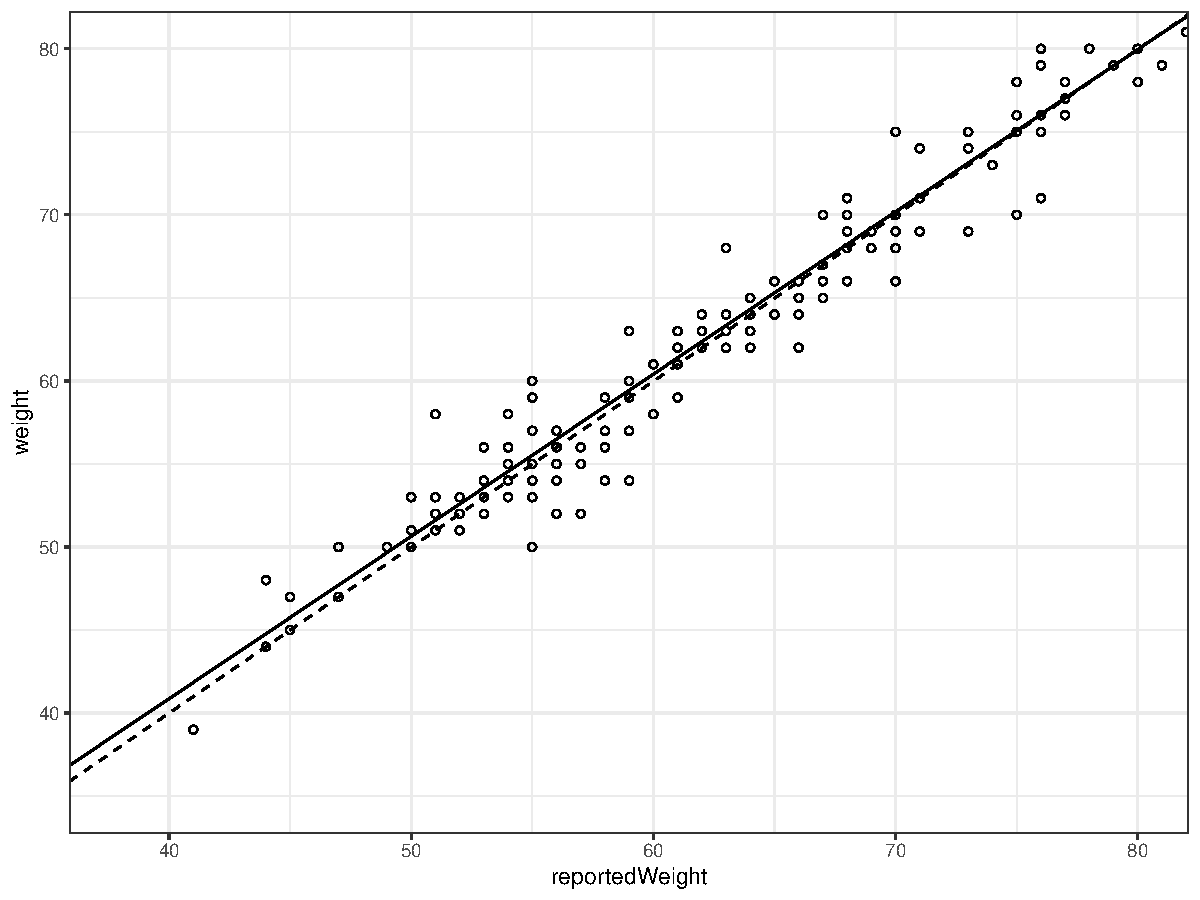
\includegraphics[width=0.8\textwidth]{Lecture3/figure_5_1.pdf}
%  \captionsetup{labelformat=empty}
  \caption{Scatterplot of Davis's data on the measured and reported weight of $101$ women.  The dashed line gives $y = x$.}
  \label{fig:weights}
\end{center}
\end{figure}

It's reasonable to assume that the relationship between measured and reported weight appears to be linear.
Denote:
\begin{itemize}
  \item measured weight by $y_i$: {\bf response variable} or {\bf dependent variable}
  \item reported weight by $x_i$: {\bf predictor variable} or {\bf independent variable}
  \item intercept: $\beta_0$ %= \Expected{y | x = 0
  \item slope: $\beta_1$
  \item residual/error term $\epsilon_i$.
\end{itemize}
%
Then the simple linear regression model writes:
$$
y_i = \beta_0 + \beta_1 x_i + \epsilon_i.
$$
For given $(\hat{\beta}_0, \hat{\beta}_1)$ values, the {\it fitted value} or {\it predicted value} for observation $i$ is:
$$
\hat{y}_i = \hat{\beta}_0 + \hat{\beta}_1 x_i.
$$
%
Therefore, the residual is
$$
\epsilon_i = y_i - \hat{y}_i 
$$

\subsubsection*{Fitting a linear model}

Choose the ``best'' values for $\beta_0, \beta_1$ such that 
$$
SS[E] = \sum\limits_{1}^{n}\left( y_i - (\hat{\beta}_0 + \hat{\beta}_1 x_i) \right)^2 = \sum\limits_{1}^{n}(y_i - \hat{y}_i)^2 = \sum\limits_{1}^{n}\epsilon_i^2
$$
is minimized.
These are {\bf least squares} (LS) estimates:
$$
\begin{array}{l}
\hat{\beta}_0 = \bar{y} - \hat{\beta}_1 \bar{x}\\
\hat{\beta}_1 = \frac{\sum(x_i - \bar{x})(y_i - \bar{y})}{\sum(x_i - \bar{x})^2}.\\
\end{array}
$$

{\it Definition: } The line satisfying the equation
$$
y = \hat{\beta}_0 + \hat{\beta}_1 x
$$
is called the \underline{linear regression} of $y$ on $x$ which is also called the \underline{least squares line}.

For Davis's data, we have
\begin{equation*}
\begin{aligned}
n &= 101 \\
\bar{y} &= \frac{5780}{101} = 57.228\\
\bar{x} &= \frac{5731}{101} = 56.743\\
\sum(x_i - \bar{x})(y_i - \bar{y}) &= 4435.9\\
\sum(x_i - \bar{x})^2 &= 4539.3,\\
\end{aligned}
\end{equation*}
so that
\begin{equation*}
\begin{aligned}
\hat{\beta}_1 &= \frac{4435.9}{4539.3} = 0.97722\\
\hat{\beta}_0 &= 57.228 - 0.97722 \times 56.743 = 1.7776\\
\end{aligned}
\end{equation*}

\newpage
\setcounter{section}{3}


\section{Lecture 4:Jan 27}


\subsection*{Last time}
\begin{itemize}
\item Column space and Nullspace (JM Appendix A)
\item Simple Linear Regression (JF Chapter 5)
\end{itemize}


\subsection*{Today}
\begin{itemize}
\item HW1 posted, due Feb 12th
\item Simple Linear Regression (JF Chapter 5)

\end{itemize}

\subsection*{Least squares estimates}

The simple linear regression (SLR) model writes:
$$
y_i = \beta_0 + \beta_1 x_i + \epsilon_i.
$$

The least squares estimates minimizes the sum of squared error (SSE)  which is 
$$
SS[E] = \sum\limits_{1}^{n}\left( y_i - (\hat{\beta}_0 + \hat{\beta}_1 x_i) \right)^2 = \sum\limits_{1}^{n}(y_i - \hat{y}_i)^2 = \sum\limits_{1}^{n}\epsilon_i^2.
$$
The {\bf least squares} (LS) estimates (in vector form):
$$
\hat{\beta}_{ls} = \left(
\begin{array}{l}
\hat{\beta}_0\\
\hat{\beta}_1\\
\end{array}
\right) =
\left(
\begin{array}{c}
\bar{y} - \hat{\beta}_1 \bar{x}\\
\frac{\sum(x_i - \bar{x})(y_i - \bar{y})}{\sum(x_i - \bar{x})^2}\\
\end{array}
\right).
$$

{\it Definition: } The line satisfying the equation
$$
y = \hat{\beta}_0 + \hat{\beta}_1 x
$$
is called the \underline{linear regression} of $y$ on $x$ which is also called the \underline{least squares line}.

\subsection*{SLR Model in Matrix Form}

\begin{equation*}
\left[ \begin{array}{c} y_1\\ y_2 \\ \vdots \\ y_n\\ \end{array} \right] =
\left[ \begin{array}{c} \beta_0 + \beta_1 x_1\\ \beta_0 + \beta_1 x_2 \\ \vdots \\ \beta_0 + \beta_1 x_n\\ \end{array} \right] +
\left[ \begin{array}{c} \epsilon_1\\ \epsilon_2 \\ \vdots \\ \epsilon_n\\ \end{array} \right]
\end{equation*}

\begin{equation*}
\left[ \begin{array}{c} y_1\\ y_2 \\ \vdots \\ y_n\\ \end{array} \right] =
\left[ \begin{array}{cc} 1   &x_1\\ 1 & x_2 \\ \vdots & \vdots \\ 1 & x_n\\ \end{array} \right] \left[ \begin{array}{c} \beta_0\\ \beta_1 \\ \end{array} \right] +
\left[ \begin{array}{c} \epsilon_1\\ \epsilon_2 \\ \vdots \\ \epsilon_n\\ \end{array} \right]
\end{equation*}

\subsubsection*{Jargons}
\begin{itemize}
  \item $\vecc{X}$  is called the {\it design matrix}
  \item $\vecc{\beta}$ is the vector of parameters
  \item $\epsilon$ is the error vector
  \item $\vecc{Y}$ is the response vector.
\end{itemize}

\subsubsection*{The Design Matrix}

\begin{equation*}
\vecc{X}_{n \times 2} = \left[ \begin{array}{cc} 1   &x_1\\ 1 & x_2 \\ \vdots & \vdots \\ 1 & x_n\\ \end{array} \right]
\end{equation*}

\subsubsection*{Vector of Parameters}

\begin{equation*}
\vecc{\beta}_{2 \times 1} =\left[ \begin{array}{c} \beta_0\\ \beta_1 \\ \end{array} \right] 
\end{equation*}

\subsubsection*{Vector of Error terms}

\begin{equation*}
\vecc{\epsilon}_{n \times 1} =\left[ \begin{array}{c} \epsilon_1\\ \epsilon_2 \\ \vdots \\ \epsilon_n\\ \end{array} \right]
\end{equation*}

\subsubsection*{Vector of Responses}

\begin{equation*}
\vecc{Y}_{n \times 1} =\left[ \begin{array}{c} y_1\\ y_2 \\ \vdots \\ y_n\\ \end{array} \right]
\end{equation*}

\subsubsection*{Gramian Matrix}

\begin{equation*}
\vecc{X}\transpose\vecc{X} =\left[ \begin{array}{cc} n & \sum_i x_i\\ \sum_i x_i  & \sum_i x_i^2\\ \end{array} \right]
\end{equation*}

Therefore, we have

$$
\vecc{Y} = \vecc{X\beta} + \vecc{\epsilon}.
$$

Assume the Gramian matrix has full rank (which actually should be the case, why?), we want to show that 
$$
\hat{\beta}_{ls} = (\vecc{X}\transpose\vecc{X})^{-1}\vecc{X}\transpose\vecc{Y}.
$$
%
The inverse of the Gramian matrix is
$$
 (\vecc{X}\transpose\vecc{X})^{-1} = \frac{1}{n\sum_i(x_i - \bar{x})^2} \left[ \begin{array}{cc} \sum_i x_i^2 & -\sum_i x_i\\ -\sum_i x_i  & n\\ \end{array} \right]
$$
%
Now we have
\begin{equation*}
\begin{aligned}
\hat{\beta}_{ls}
=& (\vecc{X}\transpose\vecc{X})^{-1}\vecc{X}\transpose\vecc{Y}\\=&
  \frac{1}{n\sum_i(x_i - \bar{x})^2} \left[ \begin{array}{cc} \sum_i x_i^2 & -\sum_i x_i\\ -\sum_i x_i  & n\\ \end{array} \right] \left[ \begin{array}{c} \vecc{1}_n\transpose \\ \vecc{x}\transpose\\ \end{array} \right] \vecc{y} \\
=& \frac{1}{n\sum_i(x_i - \bar{x})^2} \left[ \begin{array}{cc} \sum_i x_i^2 & -\sum_i x_i\\ -\sum_i x_i  & n\\ \end{array} \right]  \left[ \begin{array}{c} \sum_i{y_i}\\ \sum_i{x_i y_i} \\ \end{array} \right] \\
=& \frac{1}{n\sum_i(x_i - \bar{x})^2} \left[ \begin{array}{c} (\sum_i x_i^2)(\sum_i y_i) -(\sum_i x_i)(\sum_i x_i y_i)\\ n\sum_i{x_i y_i} - (\sum_i x_i)(\sum_i y_i) \\ \end{array} \right]  \\
= & \left[
\begin{array}{c}
\bar{y} - \frac{\sum(x_i - \bar{x})(y_i - \bar{y})}{\sum(x_i - \bar{x})^2}\ \bar{x}\\
\frac{\sum(x_i - \bar{x})(y_i - \bar{y})}{\sum(x_i - \bar{x})^2}\\
\end{array}
\right]
\end{aligned}
\end{equation*}

\medskip

Some properties:
\begin{itemize}
  \item (a) $\sum{x_i \hat{\epsilon}_i} = 0$.
  \item (b) $\sum{\hat{y}_i \hat{\epsilon}_i} = 0$ (HW1).
\end{itemize}

{\it Proof:} 
For (a), we look at
$$
\begin{aligned}
&\vecc{X}\transpose \vecc{\hat{\epsilon}} \\
=& \vecc{X}\transpose (\vecc{Y - X\hat{\beta}}) \\
=& \vecc{X}\transpose [\vecc{Y} - \vecc{X} (\vecc{X}\transpose\vecc{X})^{-1}\vecc{X}\transpose \vecc{Y}] \\
=& \vecc{X}\transpose \vecc{Y} - \vecc{X}\transpose \vecc{X} (\vecc{X}\transpose\vecc{X})^{-1}\vecc{X}\transpose \vecc{Y} \\
=& \vecc{X}\transpose \vecc{Y} - \vecc{X}\transpose \vecc{Y}\\
=& \vecc{0}
\end{aligned}
$$


{\bf Other quantities in Matrix Form }
\subsubsection*{Fitted values}
$$
\hat{\vecc{Y}} = \left[ \begin{array}{c} \hat{y}_1\\ \hat{y}_2 \\ \vdots \\ \hat{y}_n\\ \end{array} \right] =  \left[ \begin{array}{c} \hat{\beta}_0 + \hat{\beta}_1 x_1\\  \hat{\beta}_0 + \hat{\beta}_1 x_2 \\ \vdots \\  \hat{\beta}_0 + \hat{\beta}_1 x_n\\ \end{array} \right]
=  \left[ \begin{array}{cc} 1   &x_1\\ 1 & x_2 \\ \vdots & \vdots \\ 1 & x_n\\ \end{array} \right] \left[ \begin{array}{c} \hat{\beta}_0\\ \hat{\beta}_1 \\ \end{array} \right]  = X\hat{\beta}
$$

\subsubsection*{Hat matrix}
$$
\begin{aligned}
\hat{\vecc{Y}} =& \vecc{X \hat{\beta}}\\
\hat{\vecc{Y}} =& \vecc{X} (\vecc{X}\transpose\vecc{X})^{-1}\vecc{X}\transpose\vecc{Y}\\
\hat{\vecc{Y}} =& \vecc{HY}\\
\end{aligned}
$$
%
where $\vecc{H} = \vecc{X} (\vecc{X}\transpose\vecc{X})^{-1}\vecc{X}\transpose$ is called ``hat matrix'' because it turns $\vecc{Y}$ into $\hat{\vecc{Y}}$.

\subsection*{Davis's data example}
For Davis's data, we have
\begin{equation*}
\begin{aligned}
n &= 101 \\
\bar{y} &= \frac{5780}{101} = 57.228\\
\bar{x} &= \frac{5731}{101} = 56.743\\
\sum(x_i - \bar{x})(y_i - \bar{y}) &= 4435.9\\
\sum(x_i - \bar{x})^2 &= 4539.3,\\
\end{aligned}
\end{equation*}
so that
\begin{equation*}
\begin{aligned}
\hat{\beta}_1 &= \frac{4435.9}{4539.3} = 0.97722\\
\hat{\beta}_0 &= 57.228 - 0.97722 \times 56.743 = 1.7776\\
\end{aligned}
\end{equation*}

Figure~\ref{fig:updatedWeights} shows Davis's data on the measured and reported weight in kilograms of $101$ women who were engaged in regular exercise.
\begin{figure}[H]
\begin{center}
  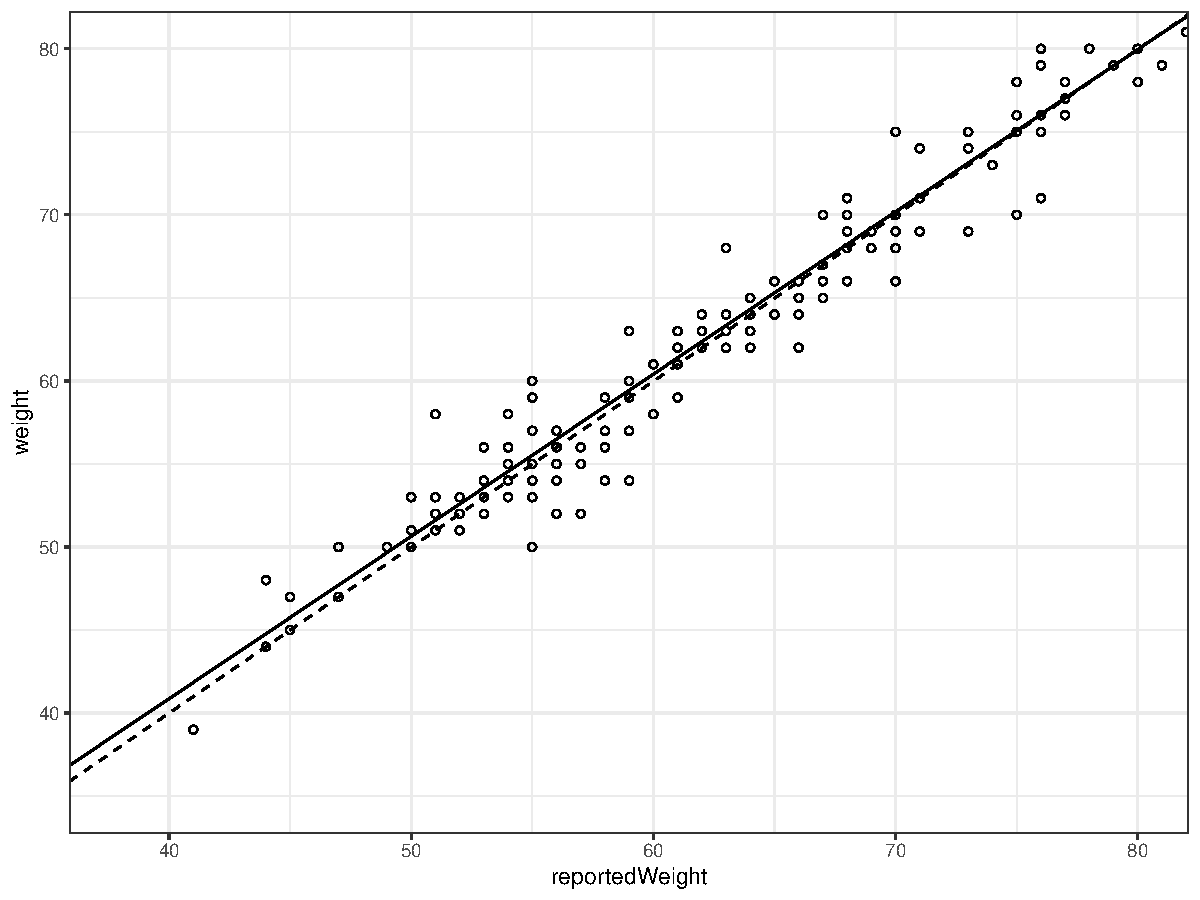
\includegraphics[width=0.8\textwidth]{Lecture3/figure_5_1.pdf}
%  \captionsetup{labelformat=empty}
  \caption{Scatterplot of Davis's data on the measured and reported weight of $101$ women.  The dashed line gives $y = x$.  The solid line gives the least squares line $y = \hat{\beta}_0 + \hat{\beta}_1 x$.}
  \label{fig:updatedWeights}
\end{center}
\end{figure}



\newpage
\setcounter{section}{5}


\section{Lecture 6:Feb 1}


\subsection*{Last time}
\begin{itemize}
\item SLR in Matrix Form
\end{itemize}


\subsection*{Today}
\begin{itemize}
\item Simple correlation
\item The statistical model of the SLR (JF chapter 6)

\end{itemize}

\section*{Simple correlation}

Having calculated the least squares line, it is of interest to determine how closely the line fits the scatter of points.
There are many ways of answering it.  The standard deviation of the residuals, $S_E$, often called the {\it standard error of the regression} or the {\it residue standard error}, provides one sort of answer.
Because of estimation considerations, the variance of the residuals is defined using {\it degrees of freedom} $n-2$:
$$
S^2_\epsilon = \frac{\sum{\hat{\epsilon}_i^2}}{n - 2}.
$$
%
The residual standard error is,
$$
S_\epsilon = \sqrt{ \frac{\sum{\hat{\epsilon}_i^2}}{n - 2}}
$$
%
For the Davis's data, the sum of squared residuals is $\sum{\epsilon_i^2} = 418.87$, and thus the standard error of the regression is
$$
S_\epsilon=\sqrt{\frac{418.87}{101 - 2}} = 2.0569 \mbox{kg}.
$$
On average, using the least-squares regression line to predict measured weight from reported weight results in an error of about $2$ kg.
%
%
\subsection*{\it Sum of squares:}
\begin{itemize}
  \item Total sum of squares (TSS) for Y: $\mbox{TSS} = \sum(y_i - \bar{y})^2$
  \item Residual sum of squares (RSS): $\mbox{RSS} = \sum(y_i - \hat{y}_i)^2$
  \item regression sum of squares (RegSS): $\mbox{RegSS} = \mbox{TSS} - \mbox{RSS} = \sum(\hat{y}_i - \bar{y})^2$
  \item $\mbox{RegSS} + \mbox{RSS} = \mbox{TSS}$
\end{itemize}

\subsection*{Sample correlation coefficient}

{\it Definition: } The \underline{sample correlation coefficient} $r_{xy}$ of the paired data $(x_1, y_1)$, $(x_2, y_2)$, ..., $(x_n, y_n)$ is defined by
$$
r_{xy} = \frac{\sum{(x_i - \bar{x})(y_i - \bar{y})}/(n - 1)}{\sqrt{\sum(x_i - \bar{x})^2/(n - 1) \times \sum(y_i - \bar{y})^2/(n - 1)}} = \frac{s_{xy}}{s_x s_y}
$$
%
$s_{xy}$ is called the sample covariance of $x$ and $y$:
$$
s_{xy} = \frac{\sum{(x_i - \bar{x})(y_i - \bar{y})}}{n - 1}
$$
$s_x = \sqrt{\sum(x_i - \bar{x})^2/(n - 1)}$ and $s_y = \sqrt{\sum(y_i - \bar{y})^2/(n - 1)}$ are, respectively, the sample standard deviations of $X$ and $Y$.

Some properties of $r_{xy}$:
\begin{itemize}
  \item $r_{xy}$ is a measure of the linear association between $x$ and $y$ in a dataset.
  \item correlation coefficients are always between $-1$ and $1$:
  $$
  -1 \le r_{xy} \le 1
  $$
  \item The closer $r_{xy}$ is to $1$, the stronger the positive linear association between $x$ and $y$
  \item The closer $r_{xy}$ is to $-1$, the stronger the negative linear association between $x$ and $y$
  \item The bigger $|r_{xy}|$, the stronger the linear association
  \item If $|r_{xy}| = 1$, then $x$ and $y$ are said to be perfectly correlated.
  \item $\hat{\beta}_1 = \frac{\sum(x_i - \bar{x})(y_i - \bar{y})}{\sum(x_i - \bar{x})^2} = \frac{s_{xy}}{s_x^2} = r_{xy} \frac{s_y}{s_x}$
\end{itemize}



\subsection*{R-square}

The ratio of RegSS to TSS is called the {\it coefficient of determination}, or sometimes, simply ``r-square''.  it represents the proportion of variation observed in the response variable $y$ which can be ``explained'' by its linear association with $x$.

\begin{itemize}
  \item In simple linear regression, ``r-square'' is in fact equal to $r^2_{xy}$. (But this isn't the case in multiple regression.)
  \item It is also equal to the squared correlation between $y_i$ and $\hat{y}_i$. (This is the case in multiple regression.)
\end{itemize}

For Davis's regression of measured on reported weight:
$$
\begin{aligned}
\mbox{TSS} &= 4753.8\\
\mbox{RSS} &= 418.87\\
\mbox{RegSS} &=  4334.9\\
\end{aligned}
$$
Thus, 
$$
r^2 = \frac{4334.9}{4753.8} = 1 - \frac{418.87}{4753.8} =0.9119
$$

\section*{The statistical model of Simple Linear Regress}

Standard statistical inference in simple regression is based on a {\it statistical model} that describes the population or process that is sampled:
$$
y_i = \beta_0 + \beta_1 x_i + \epsilon_i
$$
where the coefficients $\beta_0$ and $\beta_1$ are the {\it population regression parameters}.
The data are randomly sampled from some population of interest.
\begin{itemize}
  \item $y_i$ is the value of the response variable
  \item $x_i$ is the explanatory variable
  \item $\epsilon_i$ represents the aggregated omitted causes of $y$ (i.e.,~the causes of $y$ beyond the explanatory variable), other explanatory variables that could have been included in the regression model, measurement error in $y$, and whatever component of $y$ is inherently random.
\end{itemize}

\subsection*{Key assumptions of SLR}
The key assumptions of the SLR model concern the behavior of the errors, equivalently, the distribution of $y$ conditional on $x$:

\begin{itemize}
  \item {\it Linearity}.  The expectation of the error given the value of $x$ is $0$: $\Expected{\epsilon} \equiv \Expected{\epsilon | x_i} = 0$.  And equivalently, the expected value of the response variable is a linear function of the explanatory variable:
  $\mu_i \equiv \Expected{y_i} \equiv \Expected{y_i | x_i} = \Expected{\beta_0 + \beta_1 x_i + \epsilon_i | x_i} = \beta_0 + \beta_1 x_i$.
  \item {\it Constant variance}.  The variance of the errors is the same regardless of the value of $x$: $\Var{\epsilon | x_i} = \sigma^2_\epsilon$.  The constant error variance implies constant conditional variance of $y$ on given $x$:
  $\Var{y|x_i} = \Expected{(y_i - \mu_i)^2} = \Expected{(y_i - \beta_0 - \beta_1 x_i)^2} = \Expected{\epsilon_i^2} = \sigma^2_\epsilon$.  (Question: why the last equal sign?)
  \item {\it Normality}.  The errors are independent identically distributed with Normal distribution with mean $0$ and variance $\sigma_\epsilon^2$.  Write as $\epsilon_i \distas{iid} N(0, \sigma_\epsilon^2)$.
  Equivalently, the conditional distribution of the response variable is normal: $y_i \distas{iid} N(\beta_0 + \beta_1 x_i, \sigma_\epsilon^2)$.
  \item {\it Independence}.  The observations are sampled independently.
  \item {\it Fixed $X$, or $X$ measured without error and independent of the error}.
    \begin{itemize}
      \item For experimental research where $X$ values are under direct control of the researcher (i.e.~$X$'s are fixed).  If the experiment were replicated, then the values of $X$ would remain the same.
      \item For research where $X$ values are sampled, we assume the explanatory variable is measured without error and the explanatory variable and the error are independent in the population from which the sample is drawn.
    \end{itemize}
  \item {\it $X$ is not invariant}. X's can not be all the same.
\end{itemize}

Figure~\ref{fig:SLRdistribution} shows the assumptions of linearity, constant variance, and normality in SLR model.
\begin{figure}[H]
\begin{center}
  \includegraphics[width=0.8\textwidth]{Lecture6/Figure6-1.png}
%  \captionsetup{labelformat=empty}
  \caption{The assumptions of linearity, constant variance, and normality in simple regression.  The graph shows the conditional population distributions $\Pr(Y|x)$ of $Y$ for several values of the explanatory variable $X$, labeled as $x_1, x_2, \dots, x_5$.  The conditional means of $Y$ given $x$ are denoted $\mu_1, \dots, \mu_5$.}
  \label{fig:SLRdistribution}
\end{center}
\end{figure}


\newpage
\setcounter{section}{6}


\section{Lecture 7: Feb 3}


\subsection*{Last time}
\begin{itemize}
  \item Statistical model of SLR
\end{itemize}


\subsection*{Today}
\begin{itemize}
  \item Properties of the LS estimators
  \item Inference of SLR model
\end{itemize}



\subsection*{Properties of the Least-Squares estimator}

Under the strong assumptions of the simple regression model, the sample least squares coefficients $\hat{\beta}_{ls}$ have several desirable properties as estimators of the population regression coefficients $\beta_0$ and $\beta_1$:
\begin{itemize}
  \item The least-squares intercept and slope are {\it linear estimators}, in the sense that they are linear functions of the observations $y_i$.
  \\
  {\it Proof:\\} 
  \begin{pf}
  method (a) $\hat{\beta} = (\vecc{X}\transpose\vecc{X})^{-1} \vecc{X}\transpose\vecc{Y}$\\
  method (b) $\hat{\beta}_1 =\frac{\sum(x_i - \bar{x})(y_i - \bar{y})}{\sum(x_i - \bar{x})^2} =\frac{\sum(x_i - \bar{x})y_i}{\sum(x_i - \bar{x})^2} - \frac{\sum(x_i - \bar{x})\bar{y}}{\sum(x_i - \bar{x})^2} = \sum\frac{(x_i - \bar{x})}{\sum(x_i - \bar{x})^2}y_i = \sum k_i y_i$ where $k_i = \frac{(x_i - \bar{x})}{\sum(x_i - \bar{x})^2}$\\
  and $\hat{\beta}_0 = \bar{y} - \hat{\beta}_1 \bar{x}$
  \end{pf}
  \item The sample least-squares coefficients are {\it unbiased estimators} of the population regression coefficients:
  $$
  \begin{aligned}
  \Expected{\hat{\beta_0}} &= \beta_0\\
  \Expected{\hat{\beta_1}} &= \beta_1\\  
  \end{aligned}
  $$
  {\it Proof:} \\
  \begin{pf}
  method (a) $\Expected{\vecc{\hat{\beta}}} = \Expected{(\vecc{X}\transpose\vecc{X})^{-1} \vecc{X}\transpose\vecc{Y}} = \Expected{(\vecc{X}\transpose\vecc{X})^{-1} \vecc{X}\transpose\vecc{X\beta}} = \vecc{\beta}$.  (note: $\Expected{Y} = \Expected{\vecc{X\beta} + \vecc{\epsilon}} = \Expected{\vecc{X\beta}} + \Expected{\vecc{\epsilon}} = \vecc{X\beta}$)\\
  method (b) recall that $\hat{\beta}_1 =\sum k_i y_i$ where $k_i = \frac{(x_i - \bar{x})}{\sum(x_i - \bar{x})^2}$.  First, we want to show
  \begin{enumerate}
    \item $\sum k_i = 0$
    \item $\sum k_i x_i = 1$
  \end{enumerate}
  They are actually quite easy:  $\sum k_i = \sum_i \frac{(x_i - \bar{x})}{\sum_j (x_j - \bar{x})^2} = \frac{(\sum_i x_i) - n\bar{x}}{\sum_j(x_j - \bar{x})^2} = 0$, and 
  $\sum k_i x_i = \sum_i \frac{(x_i - \bar{x})x_i}{\sum_j(x_j - \bar{x})^2} = \frac{(\sum_i x_i^2) - \bar{x} (\sum_i x_i)}{\sum_j(x_j - \bar{x})^2} = \frac{(\sum_i x_i^2) - n \bar{x}^2}{\sum_j(x_j - \bar{x})^2} = 1$.\\
  Now $\Expected{\hat{\beta}_1} = \Expected{\sum k_i y_i} = \sum[ k_i \Expected{y_i}] = \sum[k_i (\beta_0 + \beta_1 x_i)] = \beta_0 \sum k_i + \beta_1 \sum(k_i x_i) = \beta_1$,
 and  $\Expected{\hat{\beta}_0} = \Expected{\bar{y} - \hat{\beta}_1 \bar{x}} = \Expected{\bar{y}} - \bar{x} \Expected{\hat{\beta}_1} = \Expected{\frac{1}{n}\sum y_i} - \bar{x} \beta_1 = \frac{1}{n} [\sum \Expected{y_i}] - \bar{x} \beta_1
 =  \frac{1}{n} \sum [\beta_0 + x_i \beta_1] - \bar{x} \beta_1 = \beta_0$
\end{pf}
  \item Both $\hat{\beta}_0$ and $\hat{\beta}_1$ have simple sampling variances:
  $$
  \begin{aligned}
    \sVar(\hat{\beta}_0) =& \frac{\sigma^2_\epsilon \sum{x_i^2}}{n\sum(x_i - \bar{x})^2}\\
    \sVar(\hat{\beta}_1) =& \frac{\sigma^2_\epsilon}{\sum(x_i - \bar{x})^2}\\    
  \end{aligned}
  $$
  {\it Proof:} \\
  \begin{pf}
  $\sVar(\hat{\beta}_1) = \sVar(\sum k_i y_i) = \sum k_i^2 \sVar(y_i) = \sigma_\epsilon^2 \sum k_i^2 = \sigma_\epsilon^2 \frac{\sum_i(x_i - \bar{x})^2}{[\sum_j(x_j - \bar{x})^2]^2} = \frac{\sigma^2_\epsilon}{\sum(x_i - \bar{x})^2}$, 
  and $\sVar(\hat{\beta}_0) = \sVar(\bar{y} - \hat{\beta}_1 \bar{x}) = {\rm Var} (\bar{y}) + (\bar{x})^2 {\rm Var} (\hat{\beta}_1)
    - 2 \bar{x} {\rm Cov} (\bar{Y}, \hat{\beta}_1).$\\
    Now, 
    $$
    \begin{aligned}
    {\rm Var} (\bar{y})
& = {\rm Var} \left(\frac{1}{n} \sum_{i = 1}^n y_i \right)
  = \frac{1}{n^2} \sum_{i = 1}^n {\rm Var} (y_i)
  = \frac{\sigma^2}{n},\\
  \sVar(\hat{\beta}_1) &= \frac{\sigma^2_\epsilon}{\sum(x_i - \bar{x})^2},\\
  \end{aligned}
    $$
    and 
    $$
\begin{aligned}
{\rm Cov} (\bar{Y}, \hat{\beta}_1)
 &= {\rm Cov} \left\{
     \frac{1}{n} \sum_{i = 1}^n Y_i,
     \frac{ \sum_{j = 1}^n(x_j - \bar{x})Y_j }{ \sum_{i = 1}^n(x_i - \bar{x})^2 }
     \right \} \\
 &= \frac{1}{n} \frac{ 1 }{ \sum_{i = 1}^n(x_i - \bar{x})^2 }
    {\rm Cov} \left\{ \sum_{i = 1}^n Y_i, \sum_{j = 1}^n(x_j - \bar{x})Y_j \right\} \\
 &= \frac{ 1 }{ n \sum_{i = 1}^n(x_i - \bar{x})^2 }
    \sum_{i = 1}^n (x_j - \bar{x}) \sum_{j = 1}^n {\rm Cov}(Y_i, Y_j) \\
 &= \frac{ 1 }{ n \sum_{i = 1}^n(x_i - \bar{x})^2 }
    \sum_{i = 1}^n (x_j - \bar{x}) \sigma^2 \\
 &= 0.
\end{aligned}    
    $$
    Finally, 
    $$
\begin{aligned}
{\rm Var}(\hat{\beta}_0)
 &= \frac{\sigma^2}{n} + \frac{ \sigma^2 \bar{x}^2}{ \sum_{i = 1}^n(x_i - \bar{x})^2  } \\
 &= \frac{\sigma^2 }{ n \sum_{i = 1}^n(x_i - \bar{x})^2 }
    \left\{ \sum_{i = 1}^n(x_i - \bar{x})^2 + n \bar{x}^2 \right\} \\
 &= \frac{\sigma^2 \sum_{i = 1}^n x_i^2}{ n \sum_{i = 1}^n(x_i - \bar{x})^2 }.
\end{aligned}    
    $$
\end{pf}
  \\
  \item  Rewrite the formula for $  \sVar(\hat{\beta}_1) = \frac{\sigma_\epsilon^2}{(n - 1)S_X^2}$, we see that the sampling variance of the slope estimate will be small when
  \begin{itemize}
    \item The error variance $\sigma_\epsilon^2$ is small
    \item The sample size $n$ is large
    \item The explanatory-variable values are spread out (i.e.~have a large variance, $S_X^2$)
  \end{itemize}
  \item (Gauss-Markov theorem) Under the assumptions of linearity, constant variance, and independence, the least-squares estimators are BLUE (Best Linear Unbiased Estimator), that is they have the smallest sampling variance and are unbiased. (show this)\\
  {\it Proof:}\\
  \begin{pf}
  Let $\widetilde{\beta}_1$ be another linear unbiased estimator such that $\widetilde{\beta}_1 = \sum c_i y_i$.  For $\widetilde{\beta}_1$ is still unbiased as above, $\Expected{\widetilde{\beta}_1} = \beta_0 \sum c_i + \beta_1 \sum c_i x_i = \beta_1$ for all $\beta_1$,
  we have $\sum c_i = 0$ and $\sum c_i x_i = 1$.\\
  $\Var{\widetilde{\beta}_1} = \sigma_\epsilon^2 \sum c_i^2$\\
  Let $c_i = k_i + d_i$, then 
  $$
  \begin{aligned}
  \Var{\widetilde{\beta}_1} =& \sigma_\epsilon^2 \sum(k_i + d_i)^2\\
   =&  \sigma_\epsilon^2 \left[ \sum{k_i}^2 + \sum{d_i}^2 + 2\sum{k_i d_i} \right] \\
   =& \Var{\hat{\beta}_1} + \sigma_\epsilon^2 \sum d_i^2 + 2 \sigma_\epsilon^2 \sum k_i d_i \\
  \end{aligned}$$\\
  Now we show the last term is $0$ to finish the proof.
  $$
  \begin{aligned}
  \sum k_i d_i &= \sum k_i (c_i - k_i) = \sum c_i k_i - \sum k_i^2\\
  &= \sum_i \left[ c_i \frac{x_i - \bar{x}}{\sum_j (x_j- \bar{x})^2}\right] - \frac{1}{\sum_i (x_i - \bar{x})^2}\\
  &= 0
  \end{aligned}
  $$
\end{pf}
  
  \item Under the full suite of assumptions, the least-squares coefficients $\hat{\beta}_0$ and $\hat{\beta}_1$ are the maximum-likelihood estimators of $\beta_0$ and $\beta_1$. 
  (show this)\\
  {\it Proof:}\\
  \begin{pf}
  The log likelihood under the full suite of assumptions is $\ell = -\log\left[(2\pi)^{\frac{n}{2}} \sigma^n_\epsilon \right] - \frac{1}{2 \sigma^2_\epsilon}(\vecc{Y} - \vecc{X\beta})\transpose(\vecc{Y} - \vecc{X\beta})$.
  Maximizing the likelihood is equivalent as minimizing $(\vecc{Y} - \vecc{X\beta})\transpose(\vecc{Y} - \vecc{X\beta}) = \vecc{\epsilon}\transpose \vecc{\epsilon}$ which is the SSE.  
  \end{pf}
  
  
  \item Under the assumption of normality, the least-squares coefficients are themselves normally distributed.  Summing up,
  $$
  \begin{aligned}
    \hat{\beta}_0 \sim& N(\beta_0, \frac{\sigma^2_\epsilon \sum{x_i^2}}{n\sum(x_i - \bar{x})^2}) \\
    \hat{\beta}_1 \sim & N(\beta_1, \frac{\sigma^2_\epsilon}{\sum(x_i - \bar{x})^2})\\
  \end{aligned}
  $$
\end{itemize}



\newpage
\setcounter{section}{7}


\section{Lecture 8: Feb 5}


\subsection*{Last time}
\begin{itemize}
  \item Properties of the LS estimators
\end{itemize}


\subsection*{Today}
\begin{itemize}
  \item Inference of SLR model
  \item Lab 1
\end{itemize}


\subsection*{Statistical inference of the SLR model}

Now we have the distribution of $\hat{\beta}_0$ and $\hat{\beta}_1$
  $$
  \begin{aligned}
    \hat{\beta}_0 \sim& N(\beta_0, \frac{\sigma^2_\epsilon \sum{x_i^2}}{n\sum(x_i - \bar{x})^2}) \\
    \hat{\beta}_1 \sim & N(\beta_1, \frac{\sigma^2_\epsilon}{\sum(x_i - \bar{x})^2}).\\
  \end{aligned}
  $$
%
However, $\sigma_\epsilon$ is never known in practice.  Instead, an {\it unbiased} estimator of $\sigma_\epsilon^2$ is given by
$$
\hat{\sigma_\epsilon}^2 = MS[E] = \frac{SS[E]}{n - 2}.
$$
%
{\it Proof:}\\
\begin{pf}
\begin{equation*}
MS[E] = \frac{ \sum(y_i - \hat{y}_i)^2}{n - 2},
\end{equation*}
we want to show $\Expected{ \sum(y_i - \hat{y}_i)^2} = \sigma_\epsilon^2 (n - 2)$.\\
LHS: $\Expected{ \sum(y_i - \hat{y}_i)^2} = \sum_i \left[ \Expected{y_i - \hat{y}_i}^2 \right]$\\
and $\mbox{E}[(y_i - \hat{y}_i)^2] = \sVar(y_i - \hat{y}_i) + [\Expected{y_i - \hat{y}_i}]^2= \sVar(y_i - \hat{y}_i) = \sVar(y_i) + \sVar(\hat{y}_i) - 2\mbox{cov}(y_i, \hat{y}_i)$
$$
\begin{aligned}
\sVar(y_i) &= \sigma_\epsilon^2\\
\sVar(\hat{y}_i) &= \sVar(\bar{y} + \hat{\beta}_1 (x_i - \bar{x}))\\
&=\sVar(\bar{y}) + (x_i - \bar{x})^2 \sVar(\hat{\beta}_1) + 2(x_i - \bar{x}) \mbox{Cov}(\bar{y}, \hat{\beta}_1)\\
\mbox{Cov}(\bar{y}, \hat{\beta}_1) &= \mbox{Cov}(\bar{y}, \sum k_i y_i)\\
 &= \sum_i \mbox{Cov}(\bar{y}, k_i y_i) \\
&= \sum_i \frac{k_i}{n} \sVar(y_i)\\
&= \frac{1}{n} \sum k_i\\
 &= 0\\
 \therefore \sVar(\hat{y}_i) &= \sVar(\bar{y}) + (x_i - \bar{x})^2 \sVar(\hat{\beta}_1) \\
 &= \frac{1}{n} \sigma^2_\epsilon + \frac{\sigma^2_\epsilon (x_i - \bar{x})^2 }{\sum(x_i - \bar{x})^2} \\
 &= \sigma^2_\epsilon \left[ \frac{1}{n} + \frac{ (x_i - \bar{x})^2 }{\sum(x_i - \bar{x})^2} \right]
\end{aligned}
$$
Now, we derive the last term $\mbox{cov}(y_i, \hat{y}_i)$:
$$
\begin{aligned}
\mbox{cov}(y_i, \hat{y}_i) &= \mbox{cov}(y_i, \bar{y} + \hat{\beta}_1 (x_i - \bar{x}))\\
&= \mbox{cov}(y_i, \frac{1}{n}\sum_j {y_j} + (x_i - \bar{x}) \sum_j k_j y_j)\\
&= \mbox{cov}(y_i, \sum_j \left[ \frac{1}{n} + (x_i - \bar{x}) k_j \right] y_j)\\
&= \sigma^2_\epsilon \left[ \frac{1}{n} + (x_i - \bar{x}) k_i \right]\\
&=\sigma^2_\epsilon \left[ \frac{1}{n} + \frac{ (x_i - \bar{x})^2 }{\sum(x_i - \bar{x})^2}\right]\\
\end{aligned}
$$
%
Therefore, we have for $i$th residue
$$
\begin{aligned}
\sVar(y_i - \hat{y}_i) &= \sVar(y_i) + \sVar(\hat{y}_i) - 2\mbox{cov}(y_i, \hat{y}_i)\\
&= \sigma_\epsilon^2 + \sigma^2_\epsilon \left[ \frac{1}{n} + \frac{ (x_i - \bar{x})^2 }{\sum(x_i - \bar{x})^2} \right] - 2 \sigma^2_\epsilon \left[ \frac{1}{n} +  \frac{ (x_i - \bar{x})^2 }{\sum(x_i - \bar{x})^2} \right] \\
&= \sigma_\epsilon^2 \left[ 1 - \frac{1}{n} -  \frac{ (x_i - \bar{x})^2 }{\sum(x_i - \bar{x})^2} \right].
\end{aligned}
$$
%
And finally, sum over $i$ we get
$$
\sum_i \sVar(y_i - \hat{y}_i) = \sigma_\epsilon^2 \sum_i  \left[ 1 - \frac{1}{n} -  \frac{ (x_i - \bar{x})^2 }{\sum(x_i - \bar{x})^2} \right] = (n - 2)\sigma_\epsilon^2
$$
\end{pf}

\subsection*{Confidence intervals}
Now we substitute $\hat{\sigma}_\epsilon^2$ into the distribution of $\hat{\beta}_0$ and $\hat{\beta}_1$
  $$
  \begin{aligned}
    \hat{\beta}_1 \sim & N(\beta_1, \frac{\sigma^2_\epsilon}{\sum(x_i - \bar{x})^2})\\
    \hat{\beta}_0 \sim& N(\beta_0, \frac{\sigma^2_\epsilon \sum{x_i^2}}{n\sum(x_i - \bar{x})^2}) \\    
  \end{aligned}
  $$
  to get the estimated standard errors:
  $$
  \begin{aligned}
  \reallywidehat{SE}(\hat{\beta}_1) &= \sqrt{\frac{MS[E]}{\sum(x_i - \bar{x})^2}}\\
    \reallywidehat{SE}(\hat{\beta}_0) &= \sqrt{MS[E] \left( \frac{1}{n} + \frac{\bar{x}^2}{\sum(x_i - \bar{x})^2} \right)}\\
  \end{aligned}
  $$
  And the $100(1 - \alpha)\%$ confidence intervals for $\beta_1$ and $\beta_0$ are given by
  $$
  \hat{\beta}_1 \pm t(n - 2, \alpha / 2) \sqrt{\frac{MS[E]}{S_{xx}}}
  $$
  $$
  \hat{\beta}_0 \pm t(n - 2, \alpha / 2) \sqrt{MS[E] \left( \frac{1}{n} + \frac{\bar{x}^2}{S_{xx}} \right)}\\
  $$
  where $S_{xx} = \sum(x_i - \bar{x})^2$

\subsubsection*{Confidence interval for $\Expected{Y|X=x_0}$}

The conditional mean $\Expected{Y|X=x_0}$ can be estimated by evaluating the regression function $\mu(x_0)$ at the estimates $\hat{\beta}_0$, $\hat{\beta}_1$.
The conditional variance of the expression isn't too difficult (already shown):
$$
\sVar(\hat{\beta}_0 + \hat{\beta}_1 x_0 | X = x_0) = \sigma^2(\frac{1}{n} + \frac{(x_0 - \bar{x})^2}{S_{xx}})
$$
This leads to a confidence interval of the form
$$
\hat{\beta}_0 + \hat{\beta}_1 x_0 \pm t(n - 2, \alpha / 2) \sqrt{MS[E] \left( \frac{1}{n} + \frac{(x_0 - \bar{x})^2}{S_{xx}} \right)}
$$

\subsubsection*{Prediction interval}
Often, prediction of the response variable $Y$ for a given value, say $x_0$, of the independent variable of interest.
In order to make statements about future values of $Y$, we need to take into account
\begin{itemize}
  \item the sampling distribution of $\hat{\beta}_0$ and $\hat{\beta}_1$
  \item the randomness of a future value $Y$.
\end{itemize}

We have seen the \underline{predicted value} of $Y$ based on the linear regression is given by $\hat{Y}_0 = \hat{\beta}_0 + \hat{\beta}_1 x_0$.

The \underline{95\% prediction interval} has the form
$$
\hat{Y}_0 \pm t(n - 2, \alpha / 2) \sqrt{MS[E] \left( 1 + \frac{1}{n} + \frac{(x_0 - \bar{x})^2}{S_{xx}} \right)}.
$$



\subsubsection*{Hypothesis test}
To test the hypothesis \fbox{$H_0: \beta_1 = \beta_{slope_0}$} that the population slope is equal to a specific value $\beta_{slope_0}$ (most commonly, the null hypothesis has $\beta_{slope_0} = 0$),
we calculate the test statistic ($T$-statistics) with $df = n - 2$
$$
t_0 = \frac{\hat{\beta_1} - \beta_{slope_0}}{\reallywidehat{SE}(\hat{\beta}_1)} \sim t_{n-2}
$$




\newpage
\setcounter{section}{8}


\section{Lecture 9: Feb 8}


\subsection*{Last time}
\begin{itemize}
  \item Inference of SLR model
  \item Lab 1
\end{itemize}


\subsection*{Today}
\begin{itemize}
  \item SLR questions
  \item Multiple Linear Regression
\end{itemize}



\subsection*{Some questions to answer using regression analysis:}

\begin{enumerate}
  \item What is the meaning, in words, of $\beta_1$?\\
    \begin{pf}
    {\it Answer: }$\beta_1$ is the population slope parameter of the SLR model that represents the amount of increase in the mean of the response variable with a unit increase of the explanatory variable.
    \end{pf}
  \item True/False: (a) $\beta_1$ is a statistic (b) $\beta_1$ is a parameter (c) $\beta_1$ is unknown.\\
    \begin{pf}
    {\it Answer: } (a) False (b) True (C) True.  In reality, the true population parameters are almost never known.  However, in simulation studies, we do know them.
    \end{pf}
  \item True/False: (a) $\hat{\beta}_1$ is a statistic (b) $\hat{\beta}_1$ is a parameter (c)$\hat{\beta}_1$ is unknown\\
    \begin{pf}
    {\it Answer: } (a) True (b) False (C) False.  $\hat{\beta}_1$ is an estimate of the population parameter $\beta_1$.
    \end{pf}
  \item Is $\hat{\beta}_1 = \beta_1$ ?\\
    \begin{pf}
      {\it Answer: } No.  However, $\Expected{\hat{\beta}_1} = \beta_1$ 
    \end{pf}
\end{enumerate}

\subsection*{Multiple linear regression}
JF 5.2+6.2\\
\begin{center}
\underline{Multiple linear regression - an example}
\end{center}
An example on the prestige, education,  and income levels of $45$ U.S. occupations (Duncan's data):
\begin{center}
\begin{tabular}{ | c | c | c | c | c |}
\hline
 & income & education & prestige \\ 
\hline
accountant      & 62 &86 &82\\
pilot &72 &76 &83\\
architect & 75 &92 &90\\
author &55  &90 & 76\\
chemist   & 64 &  86 & 90\\
minister & 21 &  84 & 87\\
professor & 64 &  93 & 93\\
dentist & 80 & 100 & 90\\
reporter &   67 &  87 & 52\\
engineer & 72 &  86 & 88\\
lawyer & 76 &  98 & 89\\
teacher & 48 &  91 & 73\\
\hline
\end{tabular}
\end{center}
``prestige'' represents the percentage of respondents in a survey who rated an occupation as ``good'' or ``excellent'' in prestige,
``education'' represents the percentage of incumbents in the occupation in the 1950 U.S. Census who were high school graduates, 
and ``income'' represents the percentage of occupational incumbents who earned incomes in excess of \$3,500.

Using the \colorbox{shadecolor}{pairs} command in R, we can look at the pairwise scatter plot between the three variables as in Figure~\ref{fig:duncan_pair}.
\begin{figure}[H]
\begin{center}
  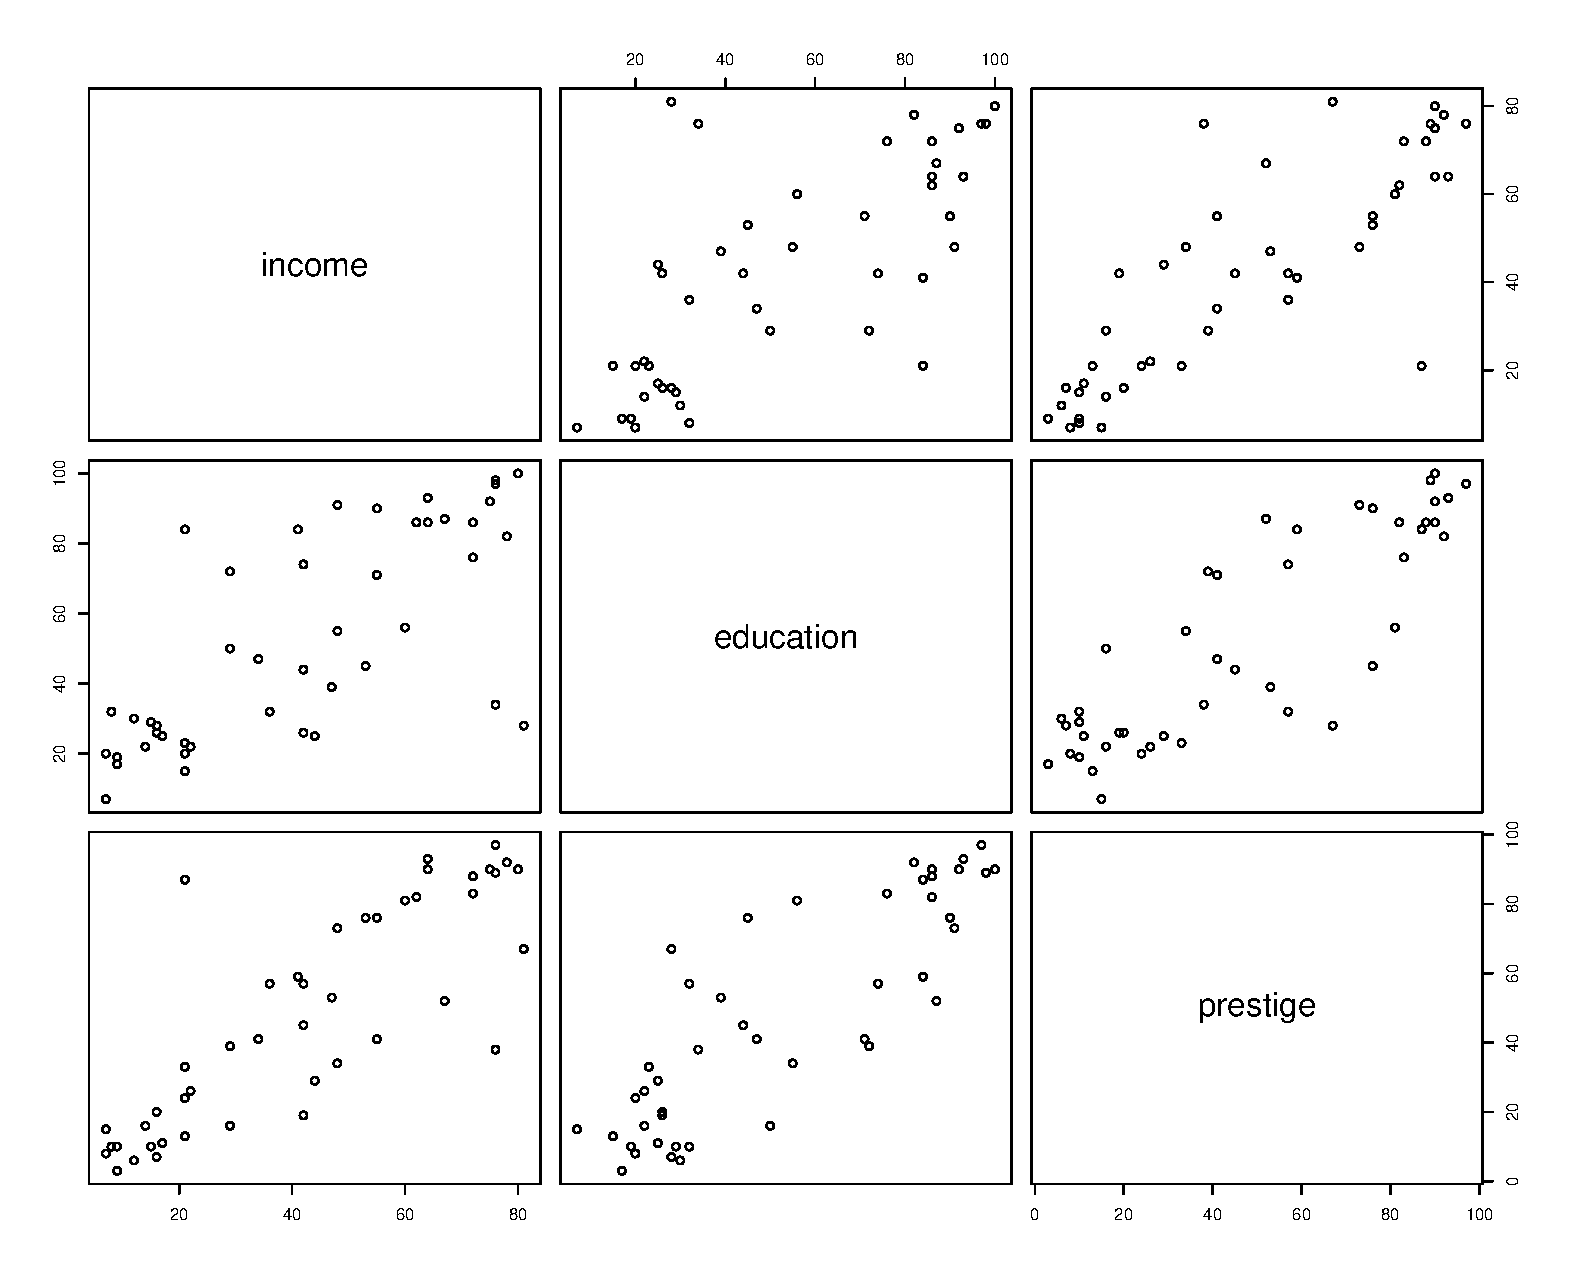
\includegraphics[width=0.8\textwidth]{Lecture9/Duncan_pairs.pdf}
  \caption{Scatterplot matrix for occupational prestige, level of education, and level of income of 45 U.S. occupations in 1950.}
  \label{fig:duncan_pair}
\end{center}
\end{figure}

Consider a regression model for the ``prestige'' of occupation $i$, $Y_i$, in which the mean of $Y_i$ is a linear function of two predictor variables $X_{i1} = income, X_{i2} = education$ for occupations $i = 1, 2,\dots, 45$:
$$
Y = \beta_0 + \beta_1 income + \beta_2 education + error
$$
or
$$
Y_i = \beta_0 + \beta_1 X_{i1} + \beta_2 X_{i2} + \epsilon_i
$$
or
$$
\begin{aligned}
Y_1 &= \beta_0 + \beta_1 X_{11} + \beta_2 X_{12} + \epsilon_1\\
Y_2 &= \beta_0 + \beta_1 X_{21} + \beta_2 X_{22} + \epsilon_2\\
\vdots &= \vdots\\
Y_{45} &= \beta_0 + \beta_1 X_{45,1} + \beta_2 X_{45,2} + \epsilon_{45}\\
\end{aligned}
$$

\subsection*{A multiple linear regression (MLR) model w/ $p$ independent variables}
Let $p$ independent variables be denoted by $x_1, \dots, x_p$.
\begin{itemize}
  \item Observed values of $p$ independent variables for $i^{th}$ subject from sample denoted by $x_{i1}, \dots, x_{ip}$
  \item response variable for $i^{th}$ subject denoted by $Y_i$
  \item For $i = 1, \dots, n$, MLR model for $Y_i$:
  $$
  Y_i = \beta_0 + \beta_1 x_{i1} + \beta_2 x_{i2} + \dots + \beta_p x_{ip} + \epsilon_i
  $$
  \item As in SLR, $\epsilon_1, \dots, \epsilon_n \distas{iid} N(0, \sigma^2)$
\end{itemize}

Least squares estimates of regression parameters minimize $SS[E]$:
$$
SS[E] = \sum\limits_{i = 1}^n (y_i - \beta_0 -  \beta_1 x_{i1} - \dots -\beta_p x_{ip})^2
$$

\begin{center}
\fbox{
$\hat{\sigma}^2 = \frac{SS[E]}{n - p - 1}$
}
\end{center}
%
Interpretations of regression parameters:
\begin{itemize}
  \item $\sigma^2$ is unknown \underline{error variance} parameter
  \item $\beta_0, \beta_1, \dots, \beta_p$ are $p + 1$ unknown regression parameters:
    \begin{itemize}
      \item $\beta_0$: average response when $x_1 = x_2 = \dots = x_p = 0$
      \item $\beta_i$ is called a \underline{partial slope} for $x_i$.  Represents mean change in $y$ per unit increase in $x_i$ {\it with all other independent variables held fixed}.
    \end{itemize}
\end{itemize}


\subsection*{Matrix formulation of MLR}
%
Let a ($1 \times (p + 1)$) vector for $p$ observed independent variables for individual $i$ be defined by 
$$
x_{i \cdot} = (1, x_{i1}, x_{i2}, \dots, x_{ip}).
$$
The MLR model for $Y_1, \dots, Y_n$ is given by
$$
\begin{aligned}
Y_1 &= \beta_0 + \beta_1 X_{11} + \beta_2 X_{12} + \dots + \beta_p X_{1p} + \epsilon_1\\
Y_2 &= \beta_0 + \beta_1 X_{21} + \beta_2 X_{22} + \dots + \beta_p X_{2p} + \epsilon_2\\
\vdots &= \vdots\\
Y_{n} &= \beta_0 + \beta_1 X_{n1} + \beta_2 X_{n2} + \dots + \beta_p X_{np} + \epsilon_{n}\\
\end{aligned}
$$
%
This system of $n$ equations can be expressed using matrices:
\begin{center}
\fbox{$\vecc{Y} = \vecc{X\beta} + \vecc{\epsilon}$}
\end{center}
%
where
\begin{itemize}
  \item $\vecc{Y}$ denotes a \underline{response vector} of size $n \times 1$
  \item $\vecc{X}$ denotes a \underline{design matrix} of size $n \times (p + 1)$
  \item $\vecc{\beta}$ denotes a vector of \underline{regression parameters} of size $(p + 1) \times 1$
  \item $\vecc{\epsilon}$ denotes an \underline{error vector} of size $n \times 1$
\end{itemize}
%
Here, the error vector $\vecc{\epsilon}$ is assumed to follow a multivariate normal distribution with variance-covariance matrix $\sigma^2 \vecc{I}_n$.
For individual $i$, 
$$
Y_i = x_{i \cdot} \beta + \epsilon_i.
$$
%
Some simplified expressions: ($\vecc{a}$ is a known $p \times 1$ vector)
\begin{subequations}
\begin{empheq}[box=\widefbox]{align*}
  \hat{\beta} &= (\vecc{X}\transpose \vecc{X})^{-1} \vecc{X}\transpose \vecc{Y}\\
  \Var{\hat{\beta}} &= \sigma^2 (\vecc{X}\transpose \vecc{X})^{-1}\\
                            &= \vecc{\Sigma}\\
  \reallywidehat{\sVar}{(\hat\beta)} &= MS[E] (\vecc{X}\transpose \vecc{X})^{-1}\\
                            &= \reallywidehat{\vecc{\Sigma}}\\
  \reallywidehat{\sVar}{(\vecc{a} \transpose \hat\beta)} &=\vecc{a} \transpose \reallywidehat{\vecc{\Sigma}} \vecc{a}\\
\end{empheq}
\end{subequations}
%
{\it Question: } what are the dimensions of each of these quantities?\\
\begin{itemize}
  \item $(\vecc{X}\transpose \vecc{X})^{-1}$ may be verbalized as `` x transposed x inverse''
  \item $\reallywidehat{\vecc{\Sigma}}$ is the estimated variance-covariance matrix for the estimate of the regression parameter vector $\vecc{\hat{\beta}}$
  \item $\vecc{X}$ is assumed to be of full {\it rank}.
\end{itemize}
%
Some more simplified expressions:
\begin{subequations}
\begin{empheq}[box=\widefbox]{align*}
  \hat{\vecc{Y}} 
  &= \vecc{X}\vecc{\hat{\beta}}\\
  &= \vecc{X} (\vecc{X}\transpose \vecc{X})^{-1} \vecc{X}\transpose \vecc{Y}\\
  &= \vecc{HY}\\
  \vecc{\hat{\epsilon}} 
  &= \vecc{Y} - \vecc{\hat{Y}}\\
  &= \vecc{Y} -  \vecc{X}\vecc{\hat{\beta}}\\
  &= (\vecc{I - H})\vecc{Y}\\
\end{empheq}
\end{subequations}
%
\begin{itemize}
  \item $\vecc{\hat{Y}}$ is called the vector of \underline{fitted} or \underline{predicted values}
  \item $\vecc{H} = \vecc{X} (\vecc{X}\transpose \vecc{X})^{-1} \vecc{X}\transpose$ is called the \underline{hat matrix}
  \item $\vecc{\hat{\epsilon}}$ is the vector of \underline{residuals}
\end{itemize}
%
For the Duncan's data example on income, education and prestige, with $p = 2$ independent variables and $n=45$ observations,
$$
\vecc{X} = \left[
\begin{tabular}{ccc}
1 & 62 &86\\
1 & 72 &76\\
\vdots&\vdots&\vdots\\
1 & 8 &  32\\
\end{tabular}
 \right]
$$
and
$$
\vecc{X}\transpose\vecc{X} = \left[
\begin{tabular}{ccc}
45 & 1884 &2365\\
1884 & 105148 &122197\\
2365 & 122197 &  163265\\
\end{tabular}
\right]
$$
$$
(\vecc{X}\transpose\vecc{X})^{-1} = \left[
\begin{tabular}{ccc}
0.10211 & -0.00085 &-0.00084\\
-0.00085 & 0.00008 &-0.00005\\
-0.00084 & -0.00005 &  0.00005\\
\end{tabular}
\right]
$$
$$
(\vecc{X}\transpose\vecc{X})^{-1} \vecc{X}\transpose \vecc{Y} = \left[
\begin{tabular}{c}
-6.0646629\\
0.5987328\\
0.5458339\\
\end{tabular}
\right] = ?
$$
$$
SS[E] = \epsilon \transpose \epsilon = (\vecc{Y} - \vecc{\hat{Y}})\transpose (\vecc{Y} - \vecc{\hat{Y}}) = 7506.7
$$
$$
MS[E] = \frac{SS[E]}{df} = \frac{7506.7}{45-2-1} = 178.73
$$
$$
\reallywidehat{\vecc{\Sigma}} = MS[E] (\vecc{X}\transpose\vecc{X})^{-1} = \left[
\begin{tabular}{ccc}
18.249481 & -0.151845008 & -0.150706025\\
-0.151845  & 0.014320275 & -0.008518551\\
-0.150706  & -0.008518551 &  0.009653582\\
\end{tabular}
\right]
$$
%



\newpage
\setcounter{section}{9}


\section{Lecture 10: Feb 10}


\subsection*{Last time}
\begin{itemize}
  \item SLR questions
  \item Multiple Linear Regression
\end{itemize}


\subsection*{Today}
\begin{itemize}
  \item Multiple correlation
  \item Confidence intervals and hypothesis tests
  \item R practice with questions
\end{itemize}



\subsection*{Multiple correlation, JF 5.2.3}
The sums of squares in multiple regression are defined in the same manner as in SLR:
$$
\begin{aligned}
  TSS =& \sum (Y_i - \bar{Y})^2\\
  RegSS =& \sum (\hat{Y}_i - \bar{Y})^2\\
  RSS =&  \sum(Y_i - \hat{Y}_i)^2 = \sum \epsilon_i^2\\
\end{aligned}
$$
%
Not surprisingly, we have a similar analysis of variance for the regression:
$$
TSS = RegSS + RSS
$$
%
The squared multiple correlation $R^2$, representing the proportion of variation in the response variable captured by the regression, is defined in terms of the sums of squares:
$$
R^2 = \frac{RegSS}{TSS} = 1 - \frac{RSS}{TSS}.
$$
Because there are several slope coefficients, potentially with different signs, the {\it multiple correlation coefficient} is, by convention, the positive square root of $R^2$.
The multiple correlation is also interpretable as the simple correlation between the fitted and observed $Y$ values, i.e.~$r_{\hat{Y}Y}$.

\subsubsection*{Adjusted-$R^2$}
Because the multiple correlation can only rise, never decline, when explanatory variables are added to the regression equation (HW1), investigators sometimes penalize the value of $R^2$ by a ``correction'' for degrees of freedom.
The corrected (or ``adjusted'') $R^2$ is defined as:
$$
\begin{aligned}
R^2_{adj} =& 1 - \frac{\frac{RSS}{n - p - 1}}{\frac{TSS}{n - 1}}\\
=& 1 - \left[ \frac{(1 - R^2)(n - 1)}{n - p - 1} \right]\\
\end{aligned}
$$

\newpage
\subsection*{Confidence intervals}
Confidence intervals and hypothesis tests for individual coefficients closely follow the pattern of simple-regression analysis:
\begin{enumerate}
  \item substitute an estimate of the error variance (MSE) for the unknown $\sigma^2$ into the variance term of $\hat{\beta}_i$
  \item find the estimated standard error of a slope coefficient $\reallywidehat{SE}(\hat{\beta}_i)$
  \item $t = \frac{\hat{\beta}_i - \beta_i}{\reallywidehat{SE}(\hat{\beta}_i)}$ follows a $t$-distribution with degrees of freedom as associated with SSE.
\end{enumerate}
Therefore, we can construct the $100(1 - \alpha)\%$ confidence interval for a single slope parameter by (why?):
$$
\hat{\beta}_i \pm t(n - p - 1, \alpha/2) \reallywidehat{SE}(\hat{\beta}_i)
$$
{\it Hand-waving proof: }\\
\begin{pf}
we know that $t = \frac{\hat{\beta}_i - \beta_i}{\reallywidehat{SE}(\hat{\beta}_i)} \sim t_{n - p - 1}$, such that
$$
\begin{aligned}
1 - \alpha =& \Pr\left( -t_c < t < t_c \right)\\
=& \Pr \left( t_c < \frac{\hat{\beta}_i - \beta_i}{\reallywidehat{SE}(\hat{\beta}_i)} < t_c \right)\\
=& \Pr \left( \hat{\beta}_i - t_c \cdot \reallywidehat{SE}(\hat{\beta}_i) < \beta_i < \hat{\beta}_i + t_c \cdot \reallywidehat{SE}(\hat{\beta}_i)  \right)\\
\end{aligned}
$$
where $t_c = t(n - p - 1, \alpha/2)$ is the critical value.  
\end{pf}

\subsection*{Hypothesis tests}
We first test the null hypothesis that all population regression slopes are $0$:
$$
H_0:\beta_1 = \beta_2 = \dots = \beta_p = 0
$$
%
The test statistics,
%
$$
F = \frac{RegSS/p}{RSS/(n-p-1)}
$$
%
follows an $F$-distribution with $p$ and $n - p -1$ degrees of freedom.

We can also test a null hypothesis about a {\it subset} of the regression slopes, e.g., 
$$
H_0: \beta_1 = \beta_2 = \dots = \beta_q = 0.
$$
Or more generally, test the null hypothesis
$$
H_0: \beta_{q_1} = \beta_{q_2} = \dots = \beta_{q_k} = 0
$$
where $0 \le q_1 < q_2 < \dots < q_k \le p$ is a subset of k indices.
To get the F-statistic for this case, we generally perform the following steps:
\begin{enumerate}
  \item Fit the {\it full} (``unconstrained'') model, in other words, model that provides context for $H_0$.  Record $SSR_{full}$ and the associated $df_{full}$
  \item Fit the {\it  reduced} (``constrained'') model, in other words, full model constrained by $H_0$.  Record $SSR_{red}$ and the associated $df_{red}$
  \item Calculate the F-statistic by 
  $$
  F = \frac{[SSR_{red} - SSR_{full}]/(df_{red} - df_{full})}{SSR_{full}/df_{full}}
  $$
  \item Find $p$-value (the probability of observing an F-statistic that is at least as high as the value that we obtained) by consulting an F-distribution with numerator $df (ndf) = df_{red} - df_{full}$ and denominator $df (ddf)= df_{full}$.
  Notation: $F_{ndf, ddf}$, see Figure~\ref{fig:p-value}.
\end{enumerate}

\begin{figure}[H]
\begin{center}
  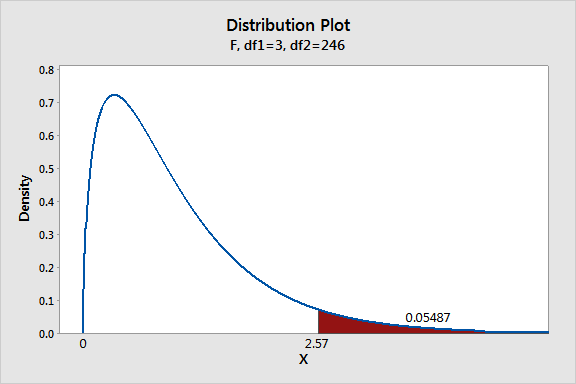
\includegraphics[width=0.8\textwidth]{Lecture10/p_value}
  \caption{An example for $p$-value for F-statistic value $2.57$ with an $F_{3, 246}$ distribution}
  \label{fig:p-value}
\end{center}
\end{figure}
%
\newpage
Now, open the \colorbox{shadecolor}{Lecture10\_to\_fill.Rmd} file and start working on the following questions:
\begin{enumerate}
  \item  What is the estimate of $\beta_1$? Interpretation?\\
  \begin{pf}
   {\it Answer: } $\hat{\beta}_1 = 0.60$ (second element of $(\vecc{X}\transpose\vecc{X})^{-1} \vecc{X}\transpose \vecc{Y}$, ``prestige'' increase per unit income for occupations with the same level of education)
  \end{pf}
  \item What is the standard error of $\hat{\beta}_1$?\\
  \begin{pf}
   {\it Answer: } $\sqrt{0.014320275} = 0.12$ (square root of middle element of $\reallywidehat{\vecc{\Sigma}}$)
   \end{pf}
  \item Is $\beta_1 = 0$ plausible, while controlling for possible linear associations between Prestige and Education? ($t(0.025, 42) = 2.02$)\\
  \begin{pf}
  {\it Answer:}  \fbox{$H_0: \beta_1 = 0$}, T-statistic: $ t = (\hat{\beta}_1 - 0)/SE(\hat{\beta}_1) = 0.60 / 0.12 = 5.0 > 2.02$,\\ (``$\hat{\beta}_1$ differs significantly from 0.'')
  \end{pf}
  \item Estimate the mean prestige among the population of ALL occupations with $income = 42$ and $education = 84$.\\
  \begin{pf}
  {\it Answer: } Unknown population mean: $\theta = \beta_0 + \beta_1 (42) + \beta_2 (84)$\\
  Estimate: $\hat{\theta} = (1, 42, 84) \vecc{\hat{\beta}} = 64.9$
  \end{pf} 
  
  \item Report a standard error\\
  \begin{pf}
   {\it Answer: } $SE(\hat{\theta}) = \sqrt{\sVar(\hat{\theta})} =  \sqrt{\sVar(\vecc{a}\transpose \hat{\beta})} = \sqrt{ \vecc{a} \transpose \reallywidehat{\vecc{\Sigma}} \vecc{a}} = 3.67$
  \end{pf}
  
  \item Report a 95\% confidence interval\\
  \begin{pf}
   {\it Answer: } $\hat{\theta} \pm t(0.025, 42) SE(\hat{\theta})$ or $64.9 \pm 2.02(3.67)$ or $(57.49, 72.31)$
  \end{pf}  
  
  \item Test the null hypothesis $H_0: \beta_1 = \beta_2 = 0$\\
  \begin{pf}
  {\it Answer: } we follow the more general formula for calculating the F-statistic:
  \begin{enumerate}
    \item  The full model $Y = \beta_0 + \beta_1 income + \beta_2 education + error$ has $SSR_{full} = 7507$ with $df_{full} = 42$.
    \item The reduced model $Y = \beta_0 + error$ has $SSR_{red} = 43688$ with $df_{red} = 40$.
    \item F-statistic: $F = \frac{[SSR_{red} - SSR_{full}]/(df_{red} - df_{full})}{SSR_{full}/df_{full}} = 101.22$
    \item use the R software to find the $p$-value: $\approx 0$
  \end{enumerate}
  \end{pf}
\end{enumerate}









\newpage
\setcounter{section}{11}


\section{Lecture 12: Feb 15}


\subsection*{Last time}
\begin{itemize}
  \item R practice with questions
\end{itemize}


\subsection*{Today}
\begin{itemize}
 \item Probability review
 \item HW2 posted
 \item HW1 review on Wednesday
\end{itemize}

\subsubsection*{Reference: }
\begin{itemize}
  \item Statistical Inference, 2nd Edition, by George Casella \& Roger L. Berger
  \item  \href{http://cs229.stanford.edu/section/cs229-prob.pdf}{Review of Probability Theory} by Arian Maleki and Tom Do
\end{itemize}

\subsection*{Probability theory review}
A few basic elements to define a probability on a set:
\begin{itemize}
  \item {\bf Sample space $S$} is the set that contains all possible outcomes of a particular experiment.
  \item An {\bf event} is any collection of possible outcomes of an experiment, that is , any subset of $S$ (including $S$ itself).
  \item Event operations
    \begin{enumerate}
      \item  Union: The union of $A$ and $B$, written $A \cup B$, is the set of elements that belong to either $A$ or $B$ or both:
      $$
      A \cup B = \{x: x \in A \mbox{ or } x \in B\}
      $$
      \item Intersection:  The intersection of $A$ and $B$, written $A \cap B$, is the set of elements that belong to both $A$ and $B$:
      $$
      A \cap B = \{ x: x \in A \mbox{ and } x \in B \}
      $$
      \item Complementation:  The complement of $A$, written as $A^c$, is the set of all elements that are not in A:
      $$
      A^c = \{x: x \notin A \}.
      $$
    \end{enumerate}
  \item {\bf Sigma algebra (or Borel field)}: A collection of subsets of $S$ is called a sigma algebra (or Borel field), denoted by $\mathcal{B}$, if it satisfies the following three properties:
    \begin{enumerate}
      \item $\emptyset \in \mathcal{B}$ (the empty set is an element of $\mathcal{B}$)
      \item If $A \in \mathcal{B}$, then $A^c \in \mathcal{B}$ ($\mathcal{B}$ is closed under complementation).
      \item If $A_1, A_2, \dots \in \mathcal{B}$, then $\cup_{i = 1}^\infty A_i \in \mathcal{B}$ ($\mathcal{B}$ is closed under countable unions).
    \end{enumerate}
  
  \item {\bf Axioms of probability: } Given a sample space $S$ and an associated sigma algebra $\mathcal{B}$, a {\it probability function} is a function $\Pr()$ with domain $\mathcal{B}$ that satisfies
    \begin{enumerate}
      \item $\Pr(A) \ge 0$ for all $A \in \mathcal{B}$
      \item $\Pr(S) = 1$.
      \item If $A_1, A_2, \dots \in \mathcal{B}$ are pairwise disjoint, then $\Pr(\cup_{i = 1}^\infty A_i) = \sum_{i = 1}^\infty \Pr(A_i)$.
    \end{enumerate} 
\end{itemize}

\subsubsection*{Properties:}
If $\Pr()$ is a {\it probability function} and $A$ and $B$ are any sets in $\mathcal{B}$, then
\begin{itemize}
  \item $\Pr(\emptyset) = 0$, where $\emptyset$ is the empty set\\
  {\it Proof: }
  \begin{pf}
  $1 = \Pr(S) = \Pr(S \cup \emptyset)$
  \end{pf}
  \item $\Pr(A) \le 1$\\
  {\it Proof: }
  \begin{pf}
   see below and remember $\Pr(A^c) \ge 0$
  \end{pf}
  \item $\Pr(A^c) = 1 - \Pr(A)$\\
  {\it Proof: }
  \begin{pf}
  $1 = \Pr(S) = \Pr(A \cup A^c) = \Pr(A ) + \Pr(A^c)$
  \end{pf}  
  \item $\Pr(B \cap A^c) = \Pr(B) - \Pr(A \cap B)$\\
  {\it Proof: }
  \begin{pf}
  $B = \{B \cap A\} \cup \{ B \cap A^c\}$
  \end{pf}
  \item $\Pr(A \cup B) = \Pr(A) + \Pr(B) - \Pr(A \cap B)$\\
  {\it Proof: }
  \begin{pf}
  $A \cup B = A \cup \{ B \cap A^c \}$ and use the above property.
  \end{pf}  
  \item $Pr(A \cup B) = \Pr(A) + \Pr(B \cap A^c) = \Pr(A) + \Pr(B) - \Pr(A \cap B)$
  \item If $A \subset B$, then $\Pr(A) \le \Pr(B)$.\\
  {\it Proof:}
  \begin{pf}
  If $A \subset B$, then $A \cap B = A$ and use $\Pr(B \cap A^c) = \Pr(B) - \Pr(A \cap B)$.
  \end{pf}
\end{itemize}

\subsubsection*{Conditional probability}
{\it Definition: } If $A$ and $B$ are events in $S$, and $\Pr(B) > 0$, then the \underline{conditional probability of $A$ given $B$}, written $\Pr(A | B)$, is
$$
\Pr(A | B) = \frac{\Pr(A \cap B)}{\Pr(B)}
$$
Note that what happens in the conditional probability calculation is that $B$ becomes the sample space: $\Pr(B|B) = 1$, in other words, 
$\Pr(A|B)$ is the probability measure of the event $A$ after observing the occurrence of event $B$.

{\it Definition: }Two events $A$ and $B$ are \underline{statistically independent} if $\Pr(A \cap B) = \Pr(A) \Pr(B)$.\\
When $A$ and $B$ are independent events, then $\Pr(A|B) = \Pr(A)$ and the following pairs are also independent
\begin{itemize}
  \item $A$ and $B^c$\\
  {\it proof: }
  \begin{pf}
  $$
  \begin{aligned}
  \Pr(A\cap B^c) &= \Pr(A) - \Pr(A \cap B)\\
  &= \Pr(A) - \Pr(A)\Pr(B)\\
  &= \Pr(A)(1 - \Pr(B))\\
  &= \Pr(A)\Pr(B^c)\\
  \end{aligned}
  $$
  \end{pf}
  \item $A^c$ and $B$
  \item $A^c$ and $B^c$
\end{itemize}

\subsection*{Random variables}
{\it Definition: } A \underline{random variable} is a function from a sample space $S$ into the real numbers.

\begin{center}
\begin{tabular}{  c c}
\hline
Experiment & Random variable\\
\hline
Toss two dice & $X = \mbox{sum of the numbers}$\\
Toss a coin $25$ times & $X = \mbox{number of heads in 25 tosses}$\\
Apply different amounts of\\ fertilizer to corn plants & $X = yield/acre$\\
\hline
\end{tabular}
\end{center}

Suppose we have a sample space
$$
S = \{ s_1, \dots, s_n\}
$$
with a probability function $\Pr$ and we define a random variable $X$ with range $\mathcal{X} = \{x_1, \dots, x_m\}$.
We can define a probability function $\Pr_X$ on $\mathcal{X}$ in the following way.
We will observe $X=x_i$ if and only if the outcome of the random experiment is an $s_j \in S$ such that $X(s_j) = x_i$.
Thus,
$$
{\Pr}_X(X = x_i) = \Pr(\{ s_j \in S: X(s_j) = x_j \}).
$$
We will simply write $\Pr(X = x_i)$ rather than ${\Pr}_X(X=x_i)$.\\
{\it A note on notation:} Randon variables are often denoted with uppercase letters and the realized values of the variables (or its range) are denoted by corresponding lowercase letters.

\subsection*{Distribution functions}
{\it Definition: } The \underline{cumulative distribution function} or \underline{\it cdf} of a random variable (r.v.) $X$, denoted by $F_X(x)$ is defined by
$$
F_X(x) = \Pr(X \le x), \mbox{ for all } x.
$$

The function $F(x)$ is a cdf if and only if the following three conditions hold:
\begin{enumerate}
  \item $\lim_{x \to \infty} F(x) = 1$.
  \item $F(x)$ is a nondecreasing function of $x$.
  \item $F(x)$ is right-continuous; that is, for every number $x_0$, $\lim_{x \downarrow x_0} = F(x_0)$.
\end{enumerate}

{\it Definition: } A random variable $X$ is \underline{continuous} if $F(x)$ is a continuous function of $x$.  A random variable $X$ is \underline{discrete} if $F(x)$ is a step function of $x$.

The following two statements are equivalent:
\begin{enumerate}
  \item The random variables $X$ and $Y$ are \underline{identically distributed}.
  \item $F_X(x) = F_Y(x)$ for every $x$.
\end{enumerate}

\subsubsection*{Density and mass functions}
{\it Definition: } The \underline{probability mass function (pmf)} of a discrete random variable $X$ is given by
$$
f_X(x) = \Pr(X = x) \mbox{ for all }x.
$$

{\small \it Example (Geometric probabilities)} For the geometric distribution, we have the pmf
$$
f_X(x) = \Pr(X = x) = \left\{ \begin{tabular}{cc}
$p{(1 - p)^{x-1}}$ & \mbox{for } x = 1, 2, \dots \\
%p(1 - p)^{x - 1} & \mbox{for } x = 1, 2, \dots\\
0 & \mbox{otherwise.}\\
\end{tabular}
\right.
$$

{\it Definition: } The \underline{probability density function} or \underline{\it pdf}, $f_X(x)$, of a continuous random variable $X$ is the function that satisfies
$$
F_X(x) = \int_{-\infty}^x f_X(t)dt \quad \mbox{ for all }x.
$$
{\it A note on notation: } The expression ``X has a distribution given by $F_X(x)$'' is abbreviated symbolically by ``$X \sim F_X(x)$'', where we read the symbol ``$\sim$'' as `` is distributed as''.

{\small \it Example (Logistic distribution)} For the logistic distribution, we have
$$
F_X(x) = \frac{1}{1 + e^{-x}}
$$
and, hence,
$$
f_X(x) = \frac{d}{dx}F_X(x) = \frac{e^{-x}}{(1 + e^{-x})^2}.
$$

A function $f_X(x)$ is a pdf (or pmf) of a random variable $X$ if and only if
\begin{enumerate}
  \item $f_X(x) \ge 0 \mbox{ for all } x$
  \item $\sum_x f_X(x) = 1\ (pmf) \quad or \quad \int_{-\infty}^{\infty} f_X(x) dx = 1\ (pdf).$
\end{enumerate}


\subsection*{Expectations}
The expected value, or expectation, of a random variable is merely its average value, where we speak of ``average'' value as one that is weighted according to the probability distribution.

{\it Definition: } The \underline{expected value} or \underline{mean} of a random variable $g(X)$, denoted by $\Expected{g(X)}$, is
$$
\Expected{g(X)} = \left\{ \begin{tabular}{ll}
$\int_{-\infty}^{\infty} g(x) f_X(x)dx$ &  if $X$ is continuous\\
$\sum_{x \in \mathcal{X}} g(x) f_X(x) = \sum_{x \in \mathcal{X}} g(x) \Pr(X = x)$ & if $X$ is discrete,\\
\end{tabular}
\right.
$$

\subsubsection*{Exponential mean}
Suppose $X \sim Exp(\lambda)$ distribution, that is, it has pdf given by
$$
f_X(x) = \frac{1}{\lambda}e^{-x/\lambda}, \quad 0\le x < \infty, \quad \lambda > 0
$$

Then $\Expected{X}$ is:\\
\begin{pf}
$$
\begin{aligned}
\Expected{X} 
&= \int_0^\infty \frac{1}{\lambda} x e^{-x/\lambda}dx\\
&= \left. -xe^{-x/\lambda} \right |_0^\infty + \int_0^\infty e^{-x/\lambda} dx\\
&= \int_0^{\infty} e^{-x/\lambda} dx = \lambda\\
\end{aligned}
$$
\end{pf}




\newpage
\setcounter{section}{12}


\section{Lecture 13: Feb 17}


\subsection*{Last time}
\begin{itemize}
  \item Probability review
\end{itemize}


\subsection*{Today}
\begin{itemize}
 \item HW1 review 
 \item Probability review, cont 
% \item 2nd-round linear algebra review
\end{itemize}

\subsubsection*{Reference: }
\begin{itemize}
  \item Statistical Inference, 2nd Edition, by George Casella \& Roger L. Berger
  \item  \href{http://cs229.stanford.edu/section/cs229-prob.pdf}{Review of Probability Theory} by Arian Maleki and Tom Do
\end{itemize}


\subsubsection*{Binomial mean}
IF $X$ has binomial distribution, i.e.~$X \sim binomial(n, p)$, its pmf is given by
$$
\Pr(X=x) = \left( \begin{tabular}{c} n\\x\\ \end{tabular} \right) p^x (1 - p)^{n - x}, \quad x=0, 1, \dots, n,
$$
%
where $n$ is a positive integer, $0 \le p \le 1$, and for every fixed pair $n$ and $p$ the pmf sums to $1$.
The expected value of a binomial random variable is then given by
$$
\Expected{X} = \sum\limits_{x=0}^{n} x \left( \begin{tabular}{c} n\\x\\ \end{tabular} \right) p^x (1 - p)^{n - x}
$$
Now, use the identity $x\left( \begin{tabular}{c} n\\x\\ \end{tabular} \right) = n \left( \begin{tabular}{c} n - 1\\ x - 1\\ \end{tabular} \right)$ to derive the Expected value.
%
\begin{pf}
$$
\begin{aligned}
\Expected{X} 
&= \sum\limits_{x=1}^{n} x \left( \begin{tabular}{c} n\\x\\ \end{tabular} \right) p^x (1 - p)^{n - x}\\
&= \sum\limits_{x=1}^{n} n \left( \begin{tabular}{c} n - 1\\ x - 1\\ \end{tabular} \right) p^x (1 - p)^{n - x}\\
&= \sum\limits_{y=0}^{n - 1} n \left( \begin{tabular}{c} n - 1\\ y\\ \end{tabular} \right) p^{y + 1} (1 - p)^{n - (y + 1)}\\
&=np \sum\limits_{y=0}^{n - 1} \left( \begin{tabular}{c} n - 1\\ y\\ \end{tabular} \right) p^{y} (1 - p)^{n - 1 - y}\\
&= np,
\end{aligned}
$$
since the last summation must be $1$, being the sum over all possible values of a $binomial(n - 1, p)$ pmf.
\end{pf}
%
\subsubsection*{properties:}
Let $X$ be a random variable and let $a, b$ and $c$ be constants. Then for any functions $g_1(x)$ and $g_2(x)$ whose expectations exist,
\begin{enumerate}
  \item $\Expected{a \cdot g_1(X)  + b \cdot g_2(X) + c} = a \Expected{g_1(X)} + b\Expected{g_2(X)} + c$.
  \item If $g_1(x) \ge 0$ for all $x$, then $\Expected{g_1(X)} \ge 0$.
  \item If $g_1(x) \ge g_2(x)$ for all x, then $\Expected{g_1(X)} \ge \Expected{g_2(X)}$.
  \item If $a \le g_1(x) \le b$ for all $x$, then $a \le \Expected{g_1(X)} \le b$.
\end{enumerate}

\subsection*{Moments}
The various moments of a distribution are an important class of expectations.

{\it Definition: } For each integer $n$, the $n^{th}$ \underline{moment} of $X$ (or $F_X(x)$), $\mu'_n$, is
$$
\mu'_n = \Expected{X^n}.
$$
The $n^{th}$ \underline{central moment} of $X$, $\mu_n$, is
$$
\mu_n = \Expected{(X-\mu)^n},
$$
where $\mu = \mu'_1 = \Expected{X}$.

\subsubsection*{Variance}
{\it Definition: } The \underline{variance} of a random variable $X$ is its second central moment, $\Var{X} = \Expected{(X - EX)^2}$.
The positive square root of $\Var{X}$ is the \underline{standard deviation} of $X$.

\subsubsection*{Exponential variance}
Let $X$ have the exponential($\lambda$) distribution, $X \sim Exp(\lambda)$.  Then the variance of $X$ is\\
%
\begin{pf}
$$
\begin{aligned}
\Var{X} &= \Expected{(X - EX)^2} = \Expected{(X - \lambda)^2}\\
&= \int_0^{\infty} (x - \lambda)^2 \frac{1}{\lambda} e^{-x/ \lambda}dx\\
&= \int_0^\infty (x^2 - 2x\lambda + \lambda^2) \frac{1}{\lambda}e^{-x / \lambda}dx\\
&= \lambda^2.
\end{aligned}
$$
\end{pf}

\subsubsection*{properties}
\begin{enumerate}
  \item $\Var{aX + b} = a^2\Var{X}$.\\
  {\it proof: }\\
  \begin{pf}
  $$
  \begin{aligned}
  \Var{aX + b} 
  &= \Expected{((aX + b) - \Expected{aX+b})^2}\\
  &= \Expected{(aX - aEX)^2}\\
  &= a^2 \Expected{(X - EX)^2}\\
  &= a^2 \Var{X}\\
  \end{aligned}
  $$  
  \end{pf}

  \item $\Var{X} = \Expected{X^2} - (\Expected{X})^2$.\\
  {\it proof: }\\
  \begin{pf}
 $$
  \begin{aligned}
  \Var{X} 
  &= \Expected{X - EX}^2\\
  &= \Expected{X^2 - 2X \Expected{X} + (\Expected{X})^2}\\
  &= \Expected{X^2} - 2\Expected{X} \Expected{X} + (\Expected{X})^2\\
  &= \Expected{X^2} -  (\Expected{X})^2\\
  \end{aligned}
  $$    
  \end{pf}  
\end{enumerate}

\subsubsection*{Moment generating function}
{\it Definition: } Let $X$ be a random variable with cdf $F_X$.  The \underline{moment generating function} or \underline{mgf} of $X$ (or $F_X$), 
denoted by $M_X(t)$, is
$$
M_X(t) = \Expected{e^{tX}},
$$
provided that the expectation exists for $t$ in some neighborhood of $0$.  That is, there exists an $h>0$ such that for all $t$ in $-h < t < h$, $\Expected{e^{tX}}$ exists.
If the expectation does not exist in a neighborhood of $0$, we say that the moment generating function does not exist.

{\it Property: } If $X$ has mgf $M_X(t)$, then
$$
\Expected{X^n} = M_X^{(n)}(0),
$$
where we define
$$
M_X^{(n)}(0) =\left. \frac{d^n}{dt^n}M_X(t) \right|_{t = 0}.
$$


\subsection*{Some common random variables}
\subsubsection*{Discrete random variables}
\begin{itemize}
  \item  $X \sim Bernoulli(p)$ (where $0 \le p \le 1$):
  $$
  \Pr(x) = \left\{ \begin{tabular}{ll} $p$ & \mbox{if } $x = 1$\\ $1 - p$ & \mbox{if } $x = 0$\\ \end{tabular} \right.
  $$
  \item  $X \sim Binomial(n, p)$ (where $0 \le p \le 1$):
  $$
  \Pr(x) = \left( \begin{tabular}{c} $n$\\ $x$\\ \end{tabular} \right) p^x (1 - p)^{n - x}
  $$ 
  \item  $X \sim Geometric(p)$ (where $0 \le p \le 1$):
  $$
  \Pr(x) = p(1 - p)^{x - 1}
  $$ 
  \item  $X \sim Poisson(\lambda)$ (where $\lambda > 0$):
  $$
  \Pr(x) = e^{-\lambda} \frac{\lambda^x}{x!}
  $$ 
\end{itemize}

\subsubsection*{Continuous random variables}
\begin{itemize}
  \item  $X \sim Uniform(a, b)$ (where $a < b$):
  $$
  f(x) = \left\{ \begin{tabular}{ll} $\frac{1}{b - a}$ & \mbox{if } $a \le x \le b$\\ $0$ & \mbox{otherwise}\\ \end{tabular} \right.
  $$ 
  \item  $X \sim Exponential(\lambda)$ (where $\lambda > 0$):
  $$
  f(x) = \left\{ \begin{tabular}{ll} $\lambda e^{-\lambda x}$ & \mbox{if } $x \ge 0$\\ $0$ & \mbox{otherwise}\\ \end{tabular} \right.
  $$   
  \item  $X \sim Normal(\mu, \sigma^2)$:
  $$
  f(x) = \frac{1}{\sqrt{2\pi}\sigma}e^{- \frac{1}{2\sigma^2}(x - \mu)^2}
  $$     
\end{itemize}

The following table provides a summary of some of the properties of these distributions.

\begin{center}
\begin{tabular}{  l l l l}
\hline
Distribution & PDF or PMF & Mean & Variance\\
\hline
$Bernoulli(p)$ & $\left\{ \begin{tabular}{ll} $p$ & \mbox{if } $x = 1$\\ $1 - p$ & \mbox{if } $x = 0$\\ \end{tabular} \right.$ &$p$& $p(1 - p)$\\
$Binomial(n,p)$ & $ \left( \begin{tabular}{c} $n$\\ $x$\\ \end{tabular} \right) p^x (1 - p)^{n - x}$ , for $0 \le k \le n$ & $np$ & $np(1 - p)$\\
$Geometric(p)$ & $ p(1 - p)^{x - 1}$, for $k = 1, 2, \dots$ & $\frac{1}{p}$ & $\frac{1 - p}{p^2}$\\ 
$Poisson(\lambda)$ & $e^{-\lambda} \frac{\lambda^x}{x!}$, for $k = 1, 2, \dots$ & $\lambda$ & $\lambda$\\
$Uniform(a, b)$ & $\frac{1}{b - a} I(a \le x \le b)$ & $\frac{a + b}{2}$ & $\frac{(b - a)^2}{12}$\\ 
$Gaussian(\mu, \sigma^2)$ & $\frac{1}{\sqrt{2\pi}\sigma}e^{- \frac{1}{2\sigma^2}(x - \mu)^2}$ &$\mu$ & $\sigma^2$\\
$Exponential(\lambda)$ & $\lambda e^{-\lambda x} I(x \ge 0)$ & $\frac{1}{\lambda}$ & $\frac{1}{\lambda^2}$\\
\hline
\label{table:distributions}
\end{tabular}
\end{center}







\newpage
\setcounter{section}{13}


\section{Lecture 14: Feb 19}


\subsection*{Last time}
\begin{itemize}
 \item HW1 review 
 \item Probability review, cont 
\end{itemize}


\subsection*{Today}
\begin{itemize}
  \item Probability review
  \item Lab session
% \item 2nd-round linear algebra review
\end{itemize}

\subsubsection*{Reference: }
\begin{itemize}
  \item Statistical Inference, 2nd Edition, by George Casella \& Roger L. Berger
  \item  \href{http://cs229.stanford.edu/section/cs229-prob.pdf}{Review of Probability Theory} by Arian Maleki and Tom Do
\end{itemize}

\subsubsection*{Chi-square, t-, and F-Distributions}
Let $Z_1, Z_2, \dots, Z_k \distas{iid} N(0, 1)$, then $X^2 \equiv Z_1^2 + Z_2^2 + \dots + Z_k^2 \sim \chi_k^2$ (with $k$ degrees of freedom).\\
If $X \sim \chi_k^2$
$$
\begin{aligned}
\Expected{X} &= k\\
\Var{X} &= 2k.\\
\end{aligned}
$$

{\bf Student's $t$ versus $\chi^2$}\\

If $X_1, \dots, X_n \distas{iid} N(\mu, \sigma^2)$, then
$$
\frac{\bar{X} - \mu}{\sigma / \sqrt{n}} \sim N(0, 1).
$$

When $\sigma$ is unknown,
$$
\frac{\bar{X} - \mu}{\hat{\sigma} / \sqrt{n}} \sim t_{n - 1}, \quad \mbox{where } \hat{\sigma} = \sqrt{\frac{\sum(X_i - \bar{X})^2}{n - 1}}.
$$
Note that
$$
\begin{aligned}
\frac{\bar{X} - \mu}{\hat{\sigma} / \sqrt{n}}
&= \frac{\bar{X} - \mu}{{\sigma} / \sqrt{n}} \cdot \frac{1}{\frac{\hat{\sigma}}{\sigma}}\\
&= Z \cdot \frac{1}{\sqrt{\frac{\sum(X_i - \bar{X})^2}{(n - 1)\sigma^2}}}\\
&= \frac{Z}{\sqrt{\frac{\chi_{n - 1}^2}{n - 1}}}
\end{aligned}
$$

{\bf $F$ versus $\chi^2$}\\

$$
F_{ndf, ddf} \equiv \frac{\chi^2_{ndf}/{ndf}}{\chi^2_{ddf}/{ddf}}
$$

{\bf $t$ versus $F$}\\

$$
\begin{aligned}
t_k &= \frac{Z}{\sqrt{\chi^2_k/k}}\\
&= \frac{\sqrt{\chi^2_1/1}}{\sqrt{\chi^2_k/k}}\\
&= \sqrt{F_{1, k}}
\end{aligned}
$$
or, in other words, $t^2_k = F_{1, k}$

\subsection*{Random vectors and matrices}
The cdf for random vector
$$
\vecc{Y} = \left[ \begin{array}{c} Y_1\\ Y_2\\ \vdots\\ Y_n\\ \end{array} \right] \mbox{ is }  F_\vecc{Y}(\vecc{y}) = \Pr(Y_1 \le y_1, Y_2 \le y_2, \dots, Y_n \le y_n)
$$
If a joint pdf exists, then $f_\vecc{Y}(\vecc{y}) = f_\vecc{Y}(y_1, \dots, y_n)$ and 
$$
 F_\vecc{Y}(\vecc{y}) = \int\limits_{-\infty}^{y_1} \int\limits_{-\infty}^{y_2} \dots \int\limits_{-\infty}^{y_n} f_\vecc{Y}(\vecc{t})d\vecc{t}
$$

\subsubsection*{Moments}
$$
\begin{aligned}
\Expected{\vecc{Y}} &= \vecc{\mu}_\vecc{Y} = \left[ \begin{array}{c} E(Y_1)\\ E(Y_2)\\ \vdots\\ E(Y_n)\\ \end{array} \right]  = \left[ \begin{array}{c} \mu_1\\ \mu_2\\ \vdots\\ \mu_n\\ \end{array} \right]\\
\Var{\vecc{Y}} 
&= \Expected{(\vecc{Y} - \vecc{\mu}_\vecc{Y})(\vecc{Y} - \vecc{\mu}_\vecc{Y})\transpose}\\
&=\Expected{ \left[ \begin{array}{lll} 
(Y_1 - \mu_1)^2 & (Y_1 - \mu_1)(Y_2 - \mu_2) & \dots\\ 
(Y_2 - \mu_2)(Y_1 - \mu_1) & (Y_2 - \mu_2)^2 & \dots\\
\dots & &\\
\end{array}\right]}\\
&= \Expected{\left[(Y_i - \mu_i)(Y_j - \mu_j), i = 1, 2, \dots, n, j = 1, 2, \dots, n \right]}\\
&= (\sigma_{ij})_{i = 1, 2, \dots, n; j = 1, 2, \dots, n}
\end{aligned}
$$
where $\sigma_{ij} = Cov(Y_i, Y_j)$

\subsubsection*{Linear functions}
Let $\vecc{X} \in \mathbb{R}^{k \times 1}, \vecc{Y} \in \mathbb{R}^{n \times 1}$ and $\vecc{A}  \in \mathbb{R}^{k \times 1}$, $\vecc{B} \in \mathbb{R}^{k \times n}$ be non-random, then
$$
\begin{aligned}
\mathop \mathbf{X}\limits_{k \times 1} &= \mathop \mathbf{A}\limits_{k \times 1} + \mathop \mathbf{B}\limits_{k \times n} \mathop \mathbf{Y}\limits_{n \times 1}\\
\Expected{ \mathbf{X}} &=  \mathbf{A} +  \mathbf{B} \Expected{\mathbf{Y}}\\
\Var{\mathbf{X}} &= \vecc{B}\Var{\vecc{Y}}\vecc{B}\transpose\\
\end{aligned}
$$

\subsubsection*{Sums of random vectors}
$$
\begin{aligned}
\mathop \mathbf{X}\limits_{n \times 1} &= \mathop \mathbf{Y}\limits_{n \times 1} +\mathop \mathbf{Z}\limits_{n \times 1}\\
\Expected{\vecc{X}} &= \Expected{\vecc{Y}} +  \Expected{\vecc{Z}} = \Expected{\vecc{Y} + \vecc{Z}}\\
\end{aligned}
$$
Note that there is no independence assumed above.
$$
\begin{aligned}
\Var{\vecc{X}} = \Var{\vecc{Y} + \vecc{Z}} = \Var{\vecc{Y}} +\Var{\vecc{Z}} + Cov(\vecc{Y}, \vecc{Z}) + Cov(\vecc{Z}, \vecc{Y})
\end{aligned}
$$
If $\vecc{Y}, \vecc{Z}$ are uncorrelated, then $\Var{\vecc{X}} = \Var{\vecc{Y}}+ \Var{\vecc{Z}}$ 





\newpage
\setcounter{section}{14}


\section{Lecture 15: Feb 22}


\subsection*{Last time}
\begin{itemize}
  \item Probability review
  \item Lab session
\end{itemize}


\subsection*{Today}
\begin{itemize}
 \item Dummy-Variable regression
 \item Interactions
% \item 2nd-round linear algebra review
\end{itemize}

\subsection*{Dummy-variable regression}
For categorical data (factor), we use dummy variable regression:
$$
Y_i = \beta_0 + \beta_1 X_{i} + \beta_2 D_{i} + \epsilon_i
$$
where $D$, called a \underline{dummy variable} regressor or an \underline{indicator variable}, is coded $1$ for one level and $0$ for all others,
$$
D_i = \left\{ \begin{array}{l l} 1 & \mbox{for men}\\ 0 & \mbox{for women}\\ \end{array} \right. .
$$
Therefore, for women, the model becomes
$$
Y_i =\beta_0 + \beta_1 X_{i} + \epsilon_i
$$
and for men
$$
Y_i = \beta_0  + \beta_1 X_{i} + \beta_2 + \epsilon_i = (\beta_0 + \beta_2) + \beta_1 X_{i} + \epsilon_i
$$

For example, Figure~\ref{fig:income_education_gender} (a) and (b) represents two small (idealized) populations.
In both cases, the within-gender regressions of income on education are parallel.
Parallel regressions imply additive effects of education and gender on income: Holding education constant, the ``effect'' of gender is the vertical distance between the two regression lines, which, for parallel lines, is everywhere the same.
%
\begin{figure}[H]
\begin{center}
  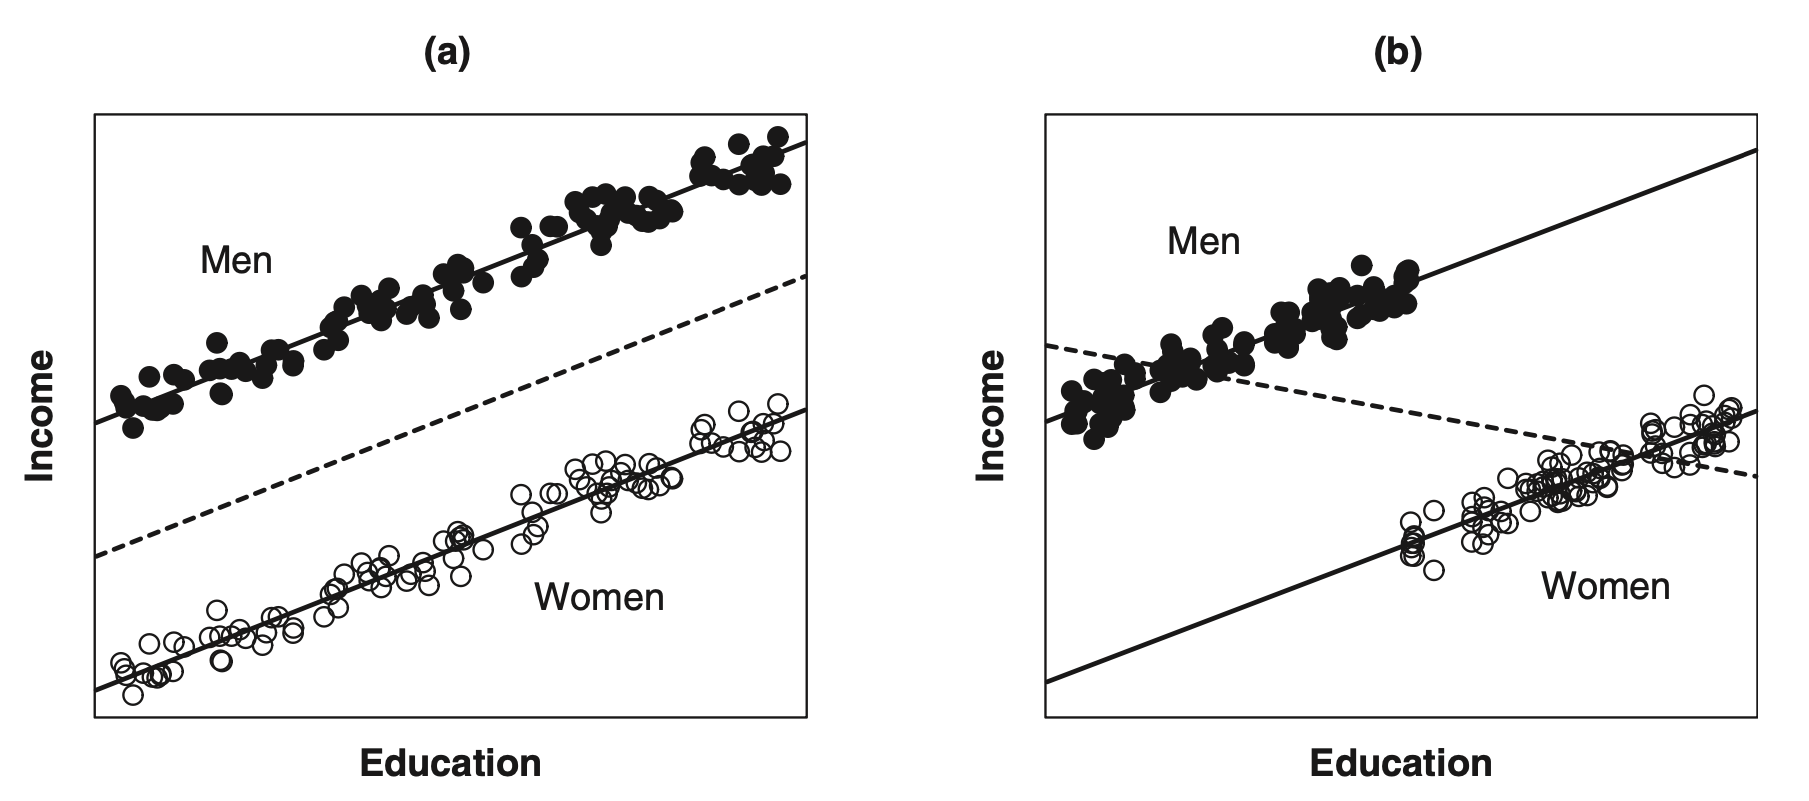
\includegraphics[width=0.8\textwidth]{Lecture15/Figure7_1}
  \caption{Idealized data representing the relationship between income and education for populations of men (filled circles) and women (open circles).  In (a), there is no relationship between education and gender; in (b), women have a higher average level of education than men.
  In both (a) and (b), the within-gender (i.e.,~partial) regressions (solid lines) are parallel.  In each graph, the overall (i.e.~marginal) regression of income on education (ignoring gender) is given by the broken line.
   JF Figure 7.1.}
  \label{fig:income_education_gender}
\end{center}
\end{figure}
%

\subsubsection*{Multi-level factor}

We can model the effects of classification factors with $m$ categories (levels) by using $m-1$ indicator variables.

For example, the three-category occupational-type factor can be represented in the regression equation by introducing two dummy regressors:
\begin{center}
\begin{tabular}{ l c c}
\hline
Category & $D_1$ & $D_2$ \\ 
\hline
Professional and managerial & 1 & 0 \\
White collar & 0 & 1 \\
Blue collar & 0 & 0 \\
\hline
\end{tabular}
\end{center}
%
A model for the regression of prestige on income, education, and type of occupation is then
$$
Y_i = \beta_0 + \beta_1 X_{i1} + \beta_2 X_{i2} + \gamma_1 D_{i1} + \gamma_2 D_{i2} + \epsilon_i
$$
%
where $X_1$ is income and $X_2$ is education.
This model describes three parallel regression planes, which can differ in their intercepts:
$$
\begin{array}{ll}
\mbox{Professional: } & Y_i = (\beta_0 + \gamma_1) + \beta_1 X_{i1} + \beta_2 X_{i2} + \epsilon_i\\
\mbox{White collar: } & Y_i = (\beta_0 + \gamma_2) + \beta_1 X_{i1} + \beta_2 X_{i2} + \epsilon_i \\
\mbox{Blue collar: } & Y_i = \beta_0 + \beta_1 X_{i1} + \beta_2 X_{i2} + \epsilon_i\\
\end{array}
$$
%
Therefore, the coeficient $\beta_0$ gives the intercept for blue-collar occupations; $\gamma_1$ represents the constant vertical difference between the parallel regression planes for professional and blue-collar occupations (fixing the values of education and income); and $\gamma_2$ represents the constant vertical distance between the regression planes for white-collar and blue-collar occupations (again, fixing education and income).

In the above prestige example, we chose ``blue collar'' as the baseline category.
Sometimes, it is natural to pick a particular category as the baseline category, for example, the ``control group'' in an experiment.
However, in most applications, the choice of a baseline category is entirely arbitrary.

\subsubsection*{Matrix representation}
For the above prestige model
$$
Y_i = \beta_0 + \beta_1 X_{i1} + \beta_2 X_{i2} + \gamma_1 D_{i1} + \gamma_2 D_{i2} + \epsilon_i
$$
we have the design matrix $\vecc{X}$ as
$$
\vecc{X} = \left[ \begin{array}{c c c c c} 
1 & X_{11} & X_{12} & D_{11} & D_{12} \\
1 & X_{21} & X_{22} & D_{21} & D_{22} \\
\vdots &\vdots & \vdots & \vdots & \vdots\\
1 & X_{n1} & X_{n2} & D_{n1} & D_{n2} \\
 \end{array}  \right]
$$
and the vector of coefficients $\vecc{\beta}$ is
$$
\vecc{\beta} = \left[ \begin{array}{c} \beta_0\\ \beta_1 \\ \beta_2 \\ \gamma_1 \\ \gamma_2 \\ \end{array} \right]
$$
such that we have (again) the linear model in matrix form:
$$
\vecc{Y} = \vecc{X\beta} + \vecc{\epsilon}
$$
where $\epsilon_i \distas{iid} N(0, \sigma^2)$, in other words,  $\vecc{\epsilon} \sim N(\vecc{0}, \sigma^2 \vecc{I}_n)$.

\subsection*{Interactions}
Two explanatory variables are said to \underline{interact} in determining a response variable when the partial effect of one depends on the value of the other.
Consider the hypothetical data shown in Figure~\ref{fig:interaction}.
%
\begin{figure}[H]
\begin{center}
  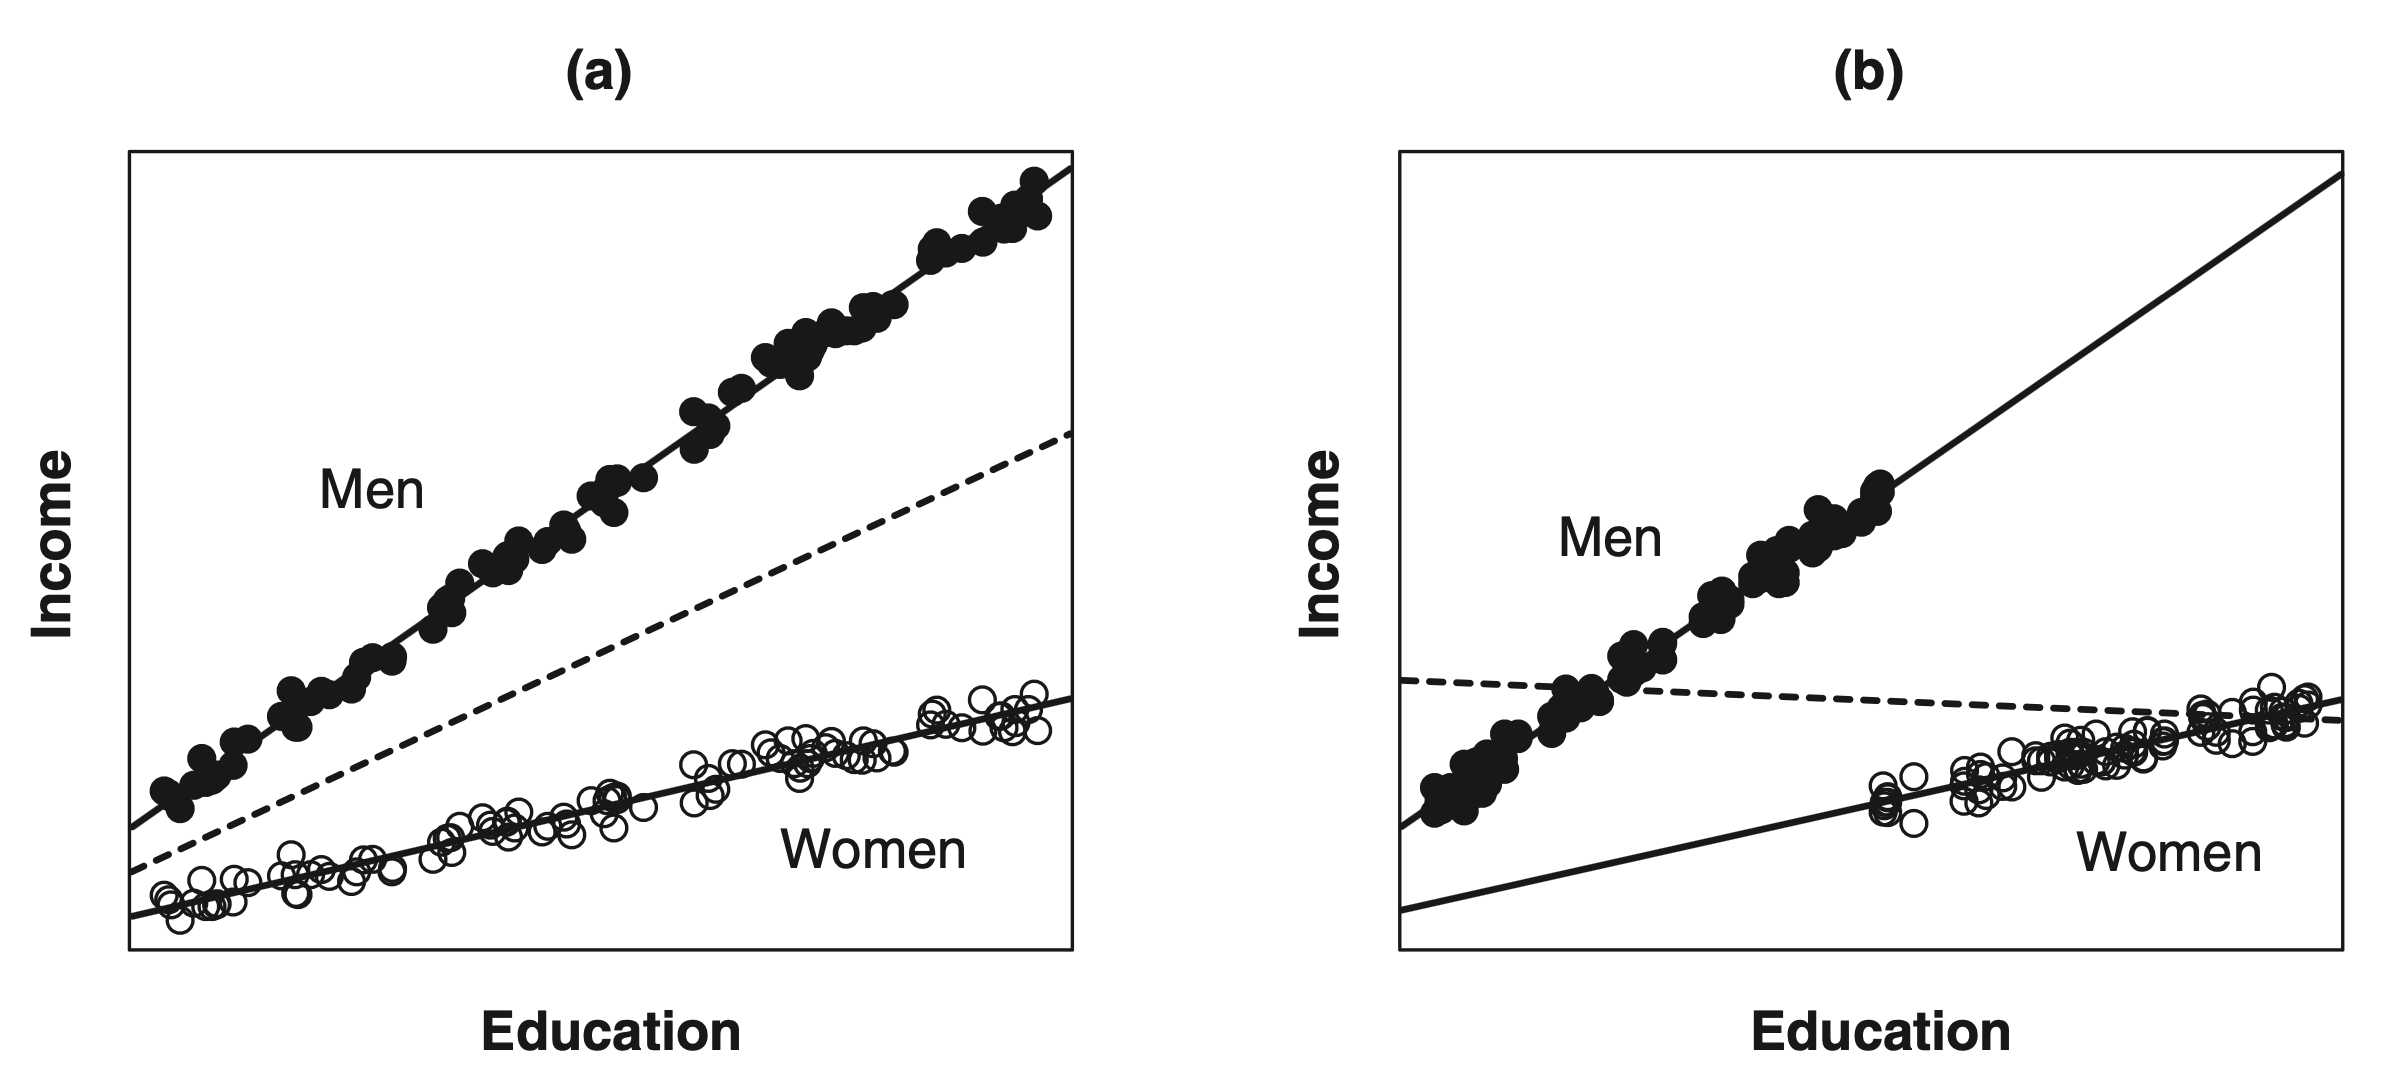
\includegraphics[width=0.8\textwidth]{Lecture15/Figure7_7}
  \caption{Idealized data representing the relationship between income and education for populations of men (filled circles) and women (open circles).
  In (a), there is no relationship between education and gender; in (b), women have a higher average level of education than men.
  In both (a) and (b), the within-gender (i.e.,~partial) regressions (solid lines) are not parallel.
  The slope for men is greater than the slope for women, and consequently education and gender interact in affecting income. 
    In each graph, the overall regression of income on education (ignoring gender) is given by the broken line.
   JF Figure 7.7.}
  \label{fig:interaction}
\end{center}
\end{figure}
%
It is apparent in both Figure~\ref{fig:interaction} (a) and (b) the within-gender regressions of income on education are not parallel: In both cases, the slope for men is larger than the slope for women.

\subsubsection*{Modeling interactions}
We accommodate the interaction of education and gender by:
$$
Y_i = \beta_0 + \beta_1 X_{i} + \beta_2 D_{i} + \beta_3 (X_i D_i) + \epsilon_i
$$
where we introduce the \underline{interaction regressor} $XD$ into the regression equation.
For women, the model becomes
$$
\begin{aligned}
Y_i &= \beta_0 + \beta_1 X_{i} + \beta_2 \cdot 0 + \beta_3 (X_i \cdot 0) + \epsilon_i\\
&= \beta_0 + \beta_1 X_i + \epsilon_i\\
\end{aligned}
$$
%
and for men
$$
\begin{aligned}
Y_i &= \beta_0 + \beta_1 X_{i} + \beta_2 \cdot 1 + \beta_3 (X_i \cdot 1) + \epsilon_i\\
&= (\beta_0 + \beta_2) + (\beta_1 + \beta_3) X_i + \epsilon_i\\
\end{aligned}
$$
The parameters $\beta_0$ and $\beta_1$ are, respectively, the intercept and slope for the regression of income on education among women (the baseline category for gender);
$\beta_2$ gives the difference in intercepts between the male and female groups;
and $\beta_3$ gives the difference in slopes between the two groups.

{\it Usual guidance: } Models that include an interaction between two predictors should also include the individual predictors by themselves regardless of the statistical significance of the associated $\beta$'s.

\subsubsection*{Test for the interaction}
We can simply test the hypothesis $H_0: \beta_3 = 0$ and construct the test statistic $t = \frac{\hat{\beta}_i - 0}{\reallywidehat{SE}(\hat{\beta}_i) } \sim t_{n - 4}$ ($p = 3$).

\subsubsection*{Interactions with multi-level factor}
We can easily extend the method for modeling interactions by forming product regressors to multi-level factors, to several factors, and to several quantitative explanatory variables.
Using the occupational prestige example, the occupational type could possibly interact both with income ($X_1$) and with education ($X_2$):
$$
\begin{aligned}
Y_i = \beta_0 &+ \beta_1 X_{i1} + \beta_2 X_{i2} + \gamma_1 D_{i1} + \gamma_2 D_{i2} \\
 &+\delta_{11} X_{i1} D_{i1} +\delta_{12} X_{i1} D_{i2} +\delta_{21} X_{i2} D_{i1} +\delta_{22} X_{i2} D_{i2} + \epsilon_i\\
\end{aligned}
$$
The model therefore permits different intercepts and slopes for the three types of occupations:
$$
\begin{array}{lrrrrr}
\mbox{Professional: } & Y_i = &(\beta_0 + \gamma_1) + &(\beta_1 + \delta_{11}) X_{i1} +& (\beta_2 + \delta_{21}) X_{i2}  +&\epsilon_i\\
\mbox{White collar: } & Y_i = &(\beta_0 + \gamma_2) + &(\beta_1 + \delta_{12}) X_{i1} +& (\beta_2 + \delta_{22}) X_{i2}  +&\epsilon_i\\
\mbox{Blue collar: } & Y_i = &\beta_0 + &\beta_1 X_{i1}+ & \beta_2 X_{i2}  +&\epsilon_i\\
\end{array}
$$












\newpage
\setcounter{section}{15}


\section{Lecture 16: Feb 24}


\subsection*{Last time}
\begin{itemize}
 \item Dummy-Variable regression (JF chapter 7)
 \item Interactions
\end{itemize}


\subsection*{Today}
\begin{itemize}
 \item Unusual and influential data (JF chapter 11)
\end{itemize}

\subsection*{Unusual and influential data}

Linear models make strong assumptions about the structure of data, assumptions that often do not hold in applications.
The method of least squares can be very sensitive to the structure of the data and may be markedly influenced by one or a few unusual observations.

\subsubsection*{Outliers}
In simple regression analysis, an \underline{outlier} is an observation whose response-variable value is {\it conditionally} unusual {\it given} the value of the explanatory variable: see Figure~\ref{fig:outlier}.
%
\begin{figure}[H]
\begin{center}
  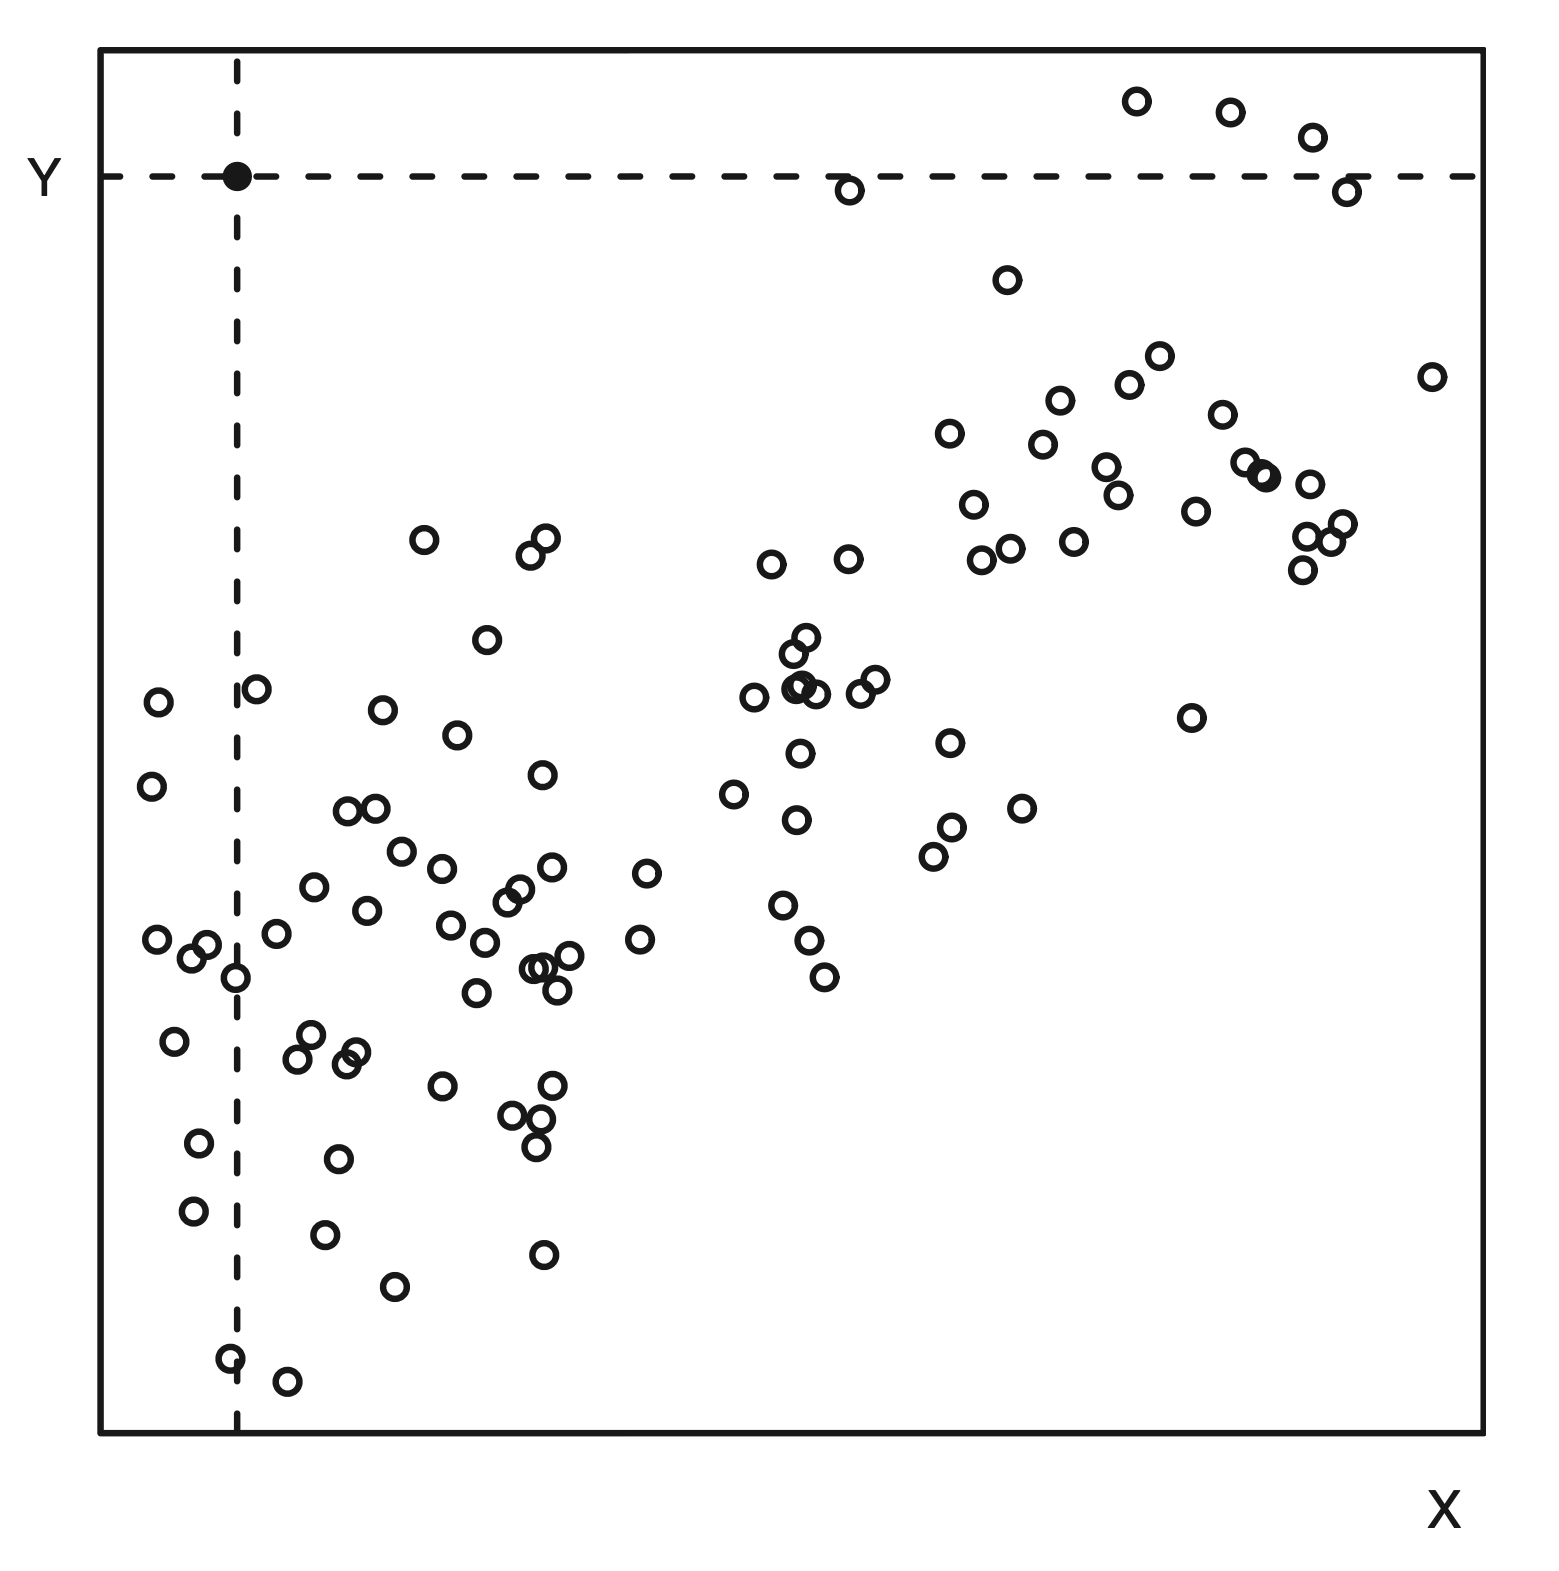
\includegraphics[width=0.4\textwidth]{Lecture16/JF_11_1}
  \caption{The black point is a regression outlier because it combines a relatively large value of $Y$ with a relatively small value of $X$, even though neither its $X$-value nor its $Y$-value is unusual individually.
  Because of the positive relationship between $Y$ and $X$, points with small $X$-values also tend to have small $Y$-values, and thus the black point is far from other points with similar $X$-values.
   JF Figure 11.1.}
  \label{fig:outlier}
\end{center}
\end{figure}
%

Unusual data are problematic in linear models fit by least squares because they can unduly influence the results of the analysis.
Their presence may be a signal that the model fails to capture important characteristics of the data.

Figure~\ref{fig:leverage_and_influence} illustrates some distinctions for the simple-regression model $Y=\beta_0 + \beta_1 X + \epsilon$.
%
\begin{figure}[H]
\begin{center}
  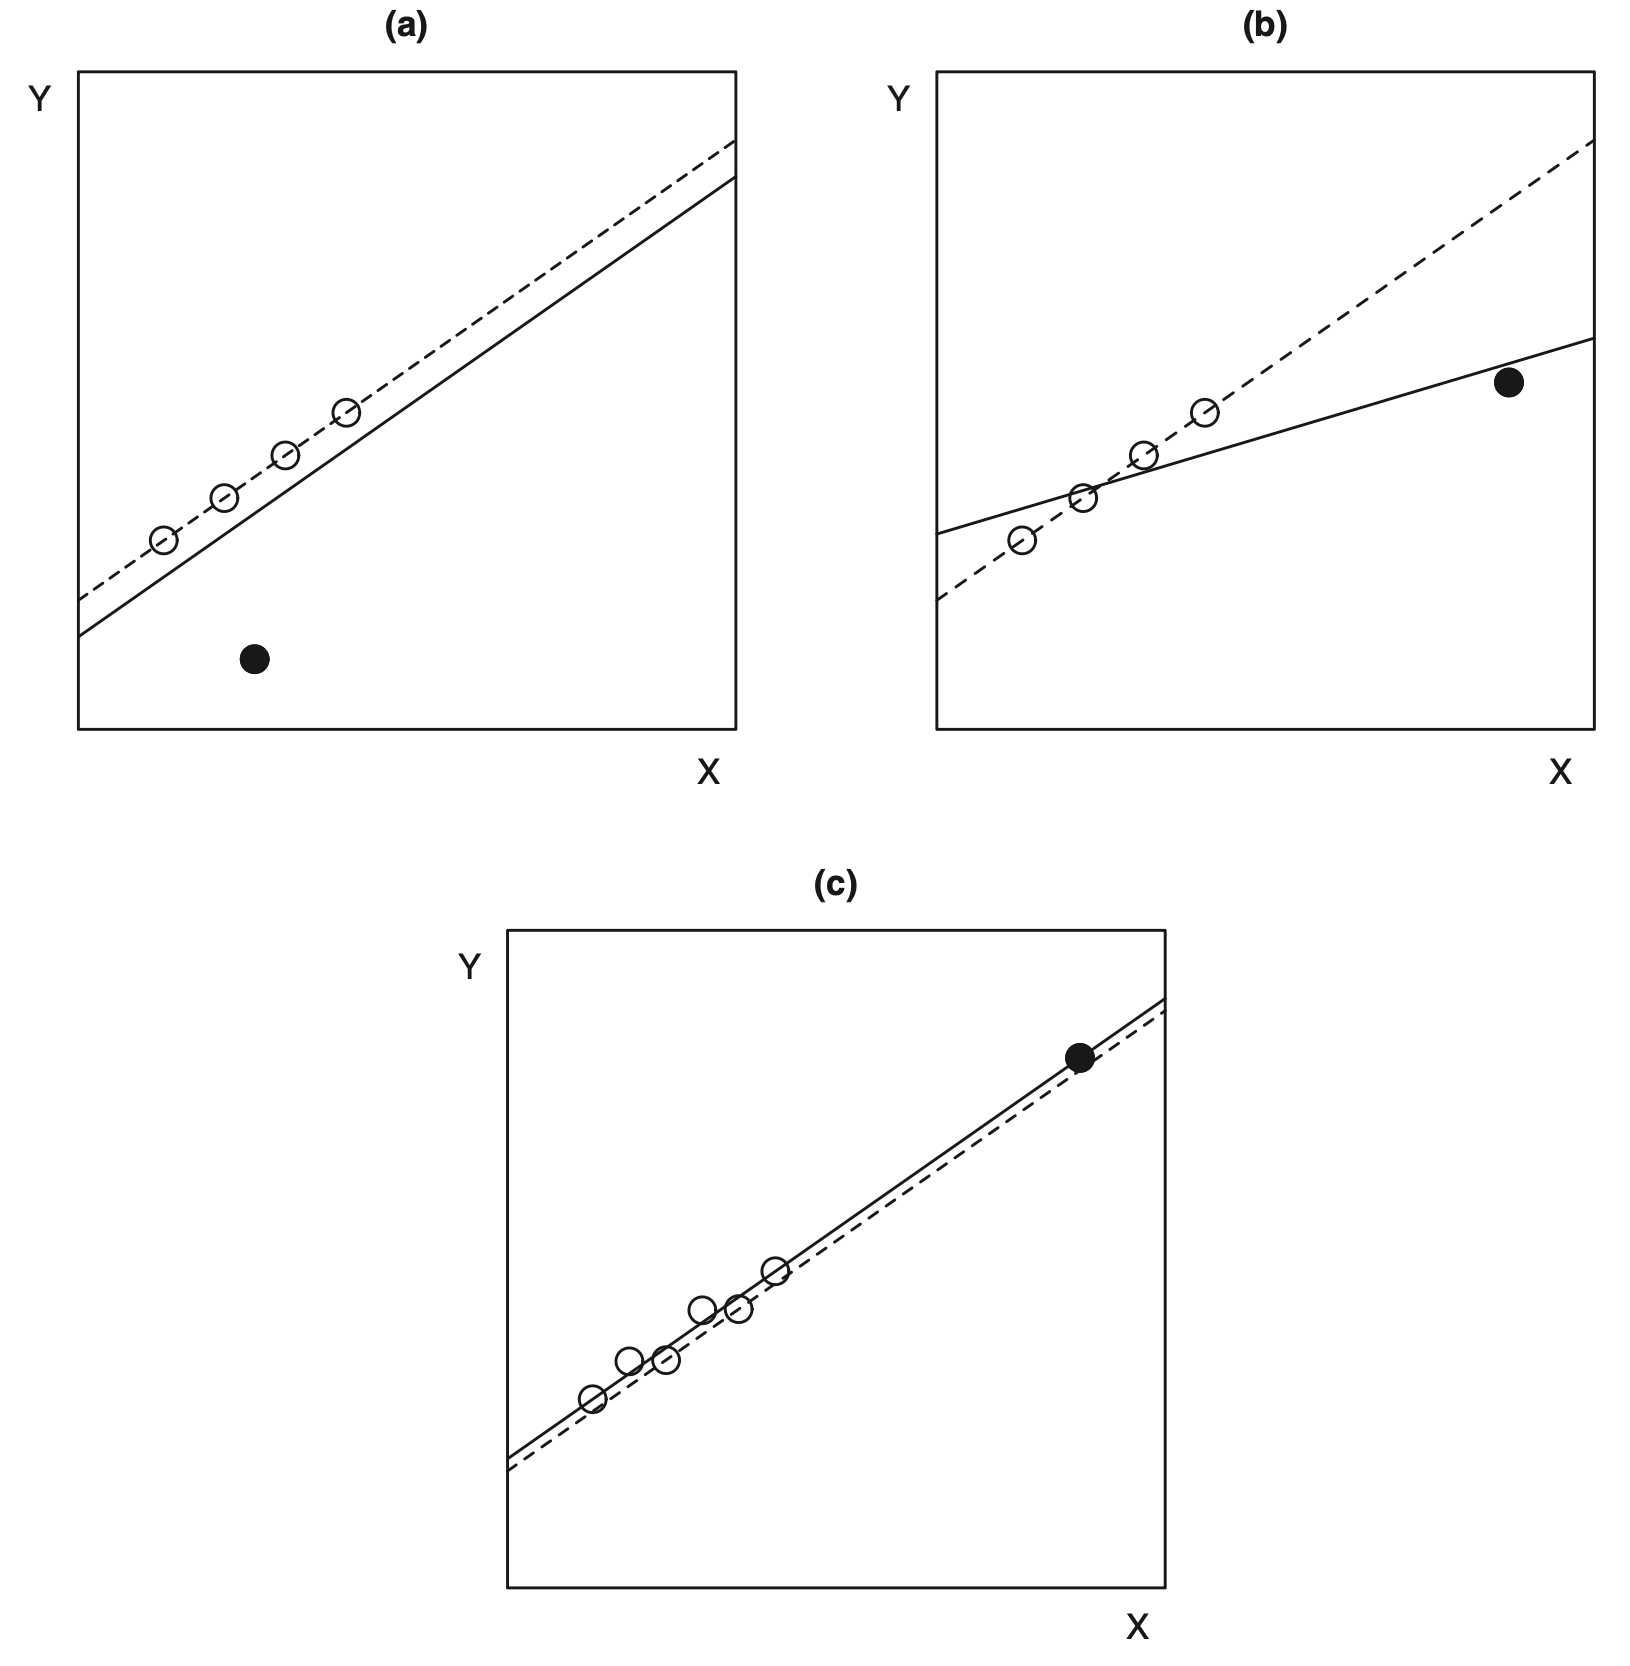
\includegraphics[width=0.8\textwidth]{Lecture16/JF_11_2}
  \caption{Leverage and influence in simple regression.
  In each graph, the solid line gives the least-squares regression for all the data, while the broken line gives the least-squares regression with the unusual data point (the black circle) omitted.
  (a) An outlier near the mean of $X$ has low leverage and little influence on the regression coefficients.
  (b) An outlier far from the mean of $X$ has high leverage and substantial influence on the regression coefficients.
  (c) A high-leverage observation in line with the rest of the data does not influence the regression coefficients.
  In panel (c), the two regression lines are separated slightly for visual effect but are, in fact, coincident
   JF Figure 11.2.}
  \label{fig:leverage_and_influence}
\end{center}
\end{figure}
%

Some qualitative distinctions between outliers and high leverage observations:
\begin{itemize}
  \item An \underline{outlier} is a data point whose response $Y$ does not follow the general trend of the rest of the data.
  \item A data point has high \underline{leverage} if it has ``extreme'' predictor $X$ values:
    \begin{itemize}
      \item With a single predictor, an extreme $X$ value is simply one that is particularly high or low.
      \item With multiple predictors, extreme $X$ values may be particularly high or low for one or more predictors, or may be ``unusual'' combinations of predictor values .
    \end{itemize}
\end{itemize}
And the \underline{influence} of a data point is the combination of leverage and discrepancy (``outlyingness'') though the following heuristic formula:
$$
\mbox{Influence on coefficients} = \mbox{Leverage} \times \mbox{Discrepancy}.
$$

\subsubsection*{Assessing leverage: hat-values}
The \underline{hat-value} $h_i$ is a common measure of leverage in regression.
They are named because it is possible to express the fitted values $\hat{Y}_j$ (``Y-hat'') in terms of the observed values $Y_i$:
$$
\hat{Y}_j = h_{1j} Y_1 + h_{2j} Y_2 + \dots + h_{jj} Y_j + \dots + h_{nj} Y_n = \sum\limits_{i = 1}^n h_{ij} Y_i.
$$
The weight $h_{ij}$ captures the contribution of observation $Y_i$ to the fitted value $\hat{Y}_j$: If $h_{ij}$ is large, then the $i$th observation can have a considerable impact on the $j$th fitted value.
With the least square solutions, for the fitted values:
$$
\hat{\vecc{Y}} = \vecc{X\beta} = \vecc{X} (\vecc{X}\transpose \vecc{X})^{-1} \vecc{X}\transpose \vecc{Y}
$$
we (already) get the \underline{hat matrix}:
$$
\vecc{H} = \vecc{X} (\vecc{X}\transpose \vecc{X})^{-1} \vecc{X}\transpose
$$

{\it Properties:}
\begin{itemize}
  \item (idempotent) $\vecc{H} = \vecc{HH}$
  \item $h_i \equiv h_{ii} = \sum_{j = 1}^n h_{ij}^2$
  \item $\frac{1}{n} \le h_{i} \le 1$    (\href{https://www.ine.pt/revstat/pdf/rs160104.pdf}{a proof} by Mohammad Mohammadi)
  \item $\bar{h} = (p + 1) / n$
\end{itemize}

In the case of SLR, the hat-values are:
$$
h_i = \frac{1}{n} + \frac{(X_i - \bar{X})^2}{\sum_{j = 1}^n (X_j - \bar{X})^2}
$$

\subsubsection*{Detecting outliers: studentized residuals}
The variance of the residuals ($\hat{\epsilon}_i = Y_i - \hat{Y}_i$) do not have equal variances (even if the errors $\epsilon_i$ have equal variances):
$$
\sVar(\hat{\epsilon}) = \sVar(\vecc{Y - X\hat{\beta}})  = \sVar[(\vecc{I - H})\vecc{Y}]= (\vecc{I - H}) \sVar(\vecc{Y})(\vecc{I - H}) = \sigma^2 (\vecc{I - H})
$$
so that for $\hat{\epsilon}_i$,
$$
\sVar(\hat{\epsilon}_i) = \sigma^2 (1 - h_i).
$$
High-leverage observations tend to have small residuals (in other words, these observations can pull the regression surface toward them).

The \underline{standardized residual} (sometimes called \underline{internally studentized residual})
$$
\hat{\epsilon}_i^{'} \equiv \frac{\hat{\epsilon}}{\hat{\sigma}\sqrt{1 - h_i}}
$$
, however, does not follow a $t$-distribution, because the numerator and denominator are not independent.

Suppose, we refit the model deleting the $i$th observation, obtaining an estimate $\hat{\sigma}_{(-i)}$ of $\sigma$ that is based on the remaining $n-1$ observations.
Then the \underline{studentized residual} (sometimes called \underline{externally studentized residual} )
$$
\hat{\epsilon}_i^{*}  \equiv \frac{\hat{\epsilon}}{\hat{\sigma}_{(-i)} \sqrt{1 - h_i}}
$$
has an independent numerator and denominator and follows a $t$-distribution with $n-p-2$ degrees of freedom.

The studentized and the standardized residuals have the following relationship (Beckman and Trussell, 1974):
$$
\hat{\epsilon}_i^{*} = \hat{\epsilon}_i' \sqrt{ \frac{n - p -2}{n - p - 1 - \hat{\epsilon}_i'^{2}}}
$$

For large $n$,
$$
\hat{\epsilon}_i^{*} \approx \hat{\epsilon}_i' \approx \frac{\hat{\epsilon}}{\hat{\sigma}}
$$

\subsubsection*{Test for outlier}
It is of our interest to pick the studentized residual $\hat{\epsilon}_{max}^{*}$ with the largest absolute value among $\hat{\epsilon}_1^{*}, \hat{\epsilon}_2^{*}, \dots, \hat{\epsilon}_n^{*}$ to test for outlier.
However, by doing so, we are effectively picking the biggest of $n$ test statistics such that it is not legitimate simply to use $t_{n - p - 2}$ to find a $p$-value.
We need a correction on the $p$-value because of multiple-comparisons.

Suppose that we have $p' = \Pr(t_{n - p - 2} > |\hat{\epsilon}_{max}^{*}|)$, the $p$-value before correction.
Then the Bonferroni adjusted $p$-value is $p = n p'$.


\subsubsection*{Measuring influence}
Influence on the regression coefficients combines leverage and discrepancy.
The most direct measure of influence simply expresses the impact on each coefficient of deleting each observation in turn:
$$
D_{ij} = \hat{\beta}_j - \tilde{\beta}_{j(-i)} \quad \mbox{for } i=1, \dots, n \mbox{ and } j=0, 1, \dots, p
$$
where $\hat{\beta}_j$ are the least-squares coefficients calculated for all the data, and the $\tilde{\beta}_{j(-i)}$ are the least-squares coefficients calculated with the $i$th observation omitted.
To assist in interpretation, it is useful to scale the $D_{ij}$ by (deleted) coefficient standard errors:
$$
D_{ij}^* = \frac{D_{ij}}{\reallywidehat{SE}_{(-i)} (\tilde{\beta}_{j(-i)})}
$$
Following Belsley, Kuh, and Welsh (1980), the $D_{ij}$ are often termed DFBETA$_{ij}$, and $D_{ij}^*$ are called DFBETAS$_{ij}$.
One problem associated with using $D_{ij}$ or  $D_{ij}^*$ is their large number $n(p+1)$ of each.

Cook's distance calculated as
$$
D_i = \frac{\sum_{j = 1}^n(\tilde{y}_{j(-i)} - \hat{y}_j )^2}{(p + 1) \hat{\sigma}^2 } = \frac{\hat{\epsilon}_i^{'2} }{p + 1} \times \frac{h_i}{1 - h_i}
$$
In effect, the first term in the formula for Cook's $D$ is a measure of discrepancy, and the second is a measure of leverage.
We look for values of $D_i$ that stand out from the rest.

A similar measure suggested by Belsley et al. (1980)
$$
\mbox{DFFITS}_i = \hat{\epsilon}_i^{*} \frac{h_i}{1 - h_i}
$$
Except for unusual data configurations, Cook's $D_i \approx \mbox{DFFITS}_i^2/(p + 1)$.

\subsubsection*{Numerical cutoffs (suggested)}

\begin{center}
\begin{tabular}{ c c}
\hline
Diagnostic statistic & Cutoff value\\
\hline
$h_i$ & $ 2 \bar{h} =  \frac{2(p + 1)}{n}$, ($3\bar{h}$ for small sample)\\
$D_{ij}^*$ & $|D_{ij}^*| > 1$ or $2$ ($2/\sqrt{n}$ for large samples)\\
Cook's $D_i$ & $D_i > \frac{4}{n - p -1}$\\
$\mbox{DFFITS}$ & $|\mbox{DFFITS}_i| > 2 \sqrt{ \frac{p + 1}{n - p - 1}}$ \\
\hline
\label{table:distributions}
\end{tabular}
\end{center}








\newpage
\setcounter{section}{16}


\section{Lecture 17: Feb 26}


\subsection*{Last time}
\begin{itemize}
 \item Unusual and influential data (JF chapter 11)
\end{itemize}


\subsection*{Today}
\begin{itemize}
 \item Added-variable plots
 \item Should unusual data be discarded
\end{itemize}



\subsection*{Added-variable plots}
Unlike the case of SLR, the scatterplot with the response variable and one predictor gives only the marginal effect in MLR.
Instead, the \underline{added-variable plot} (also called a partial-regression plot or a partial-regression leverage plot) gives a graphical inspection over each dimension.

Let $\hat{Y}_i^{(1)}$ represent the residuals from the least-squares regression of $Y$ on all the $X$s except $X_1$, in other words, the residuals from the following fitted regression equation:
$$
Y_i = \tilde{\beta}_0 ^{(1)} +  \tilde{\beta}_2^{(1)} X_{i2} + \dots +  \tilde{\beta}_p ^{(1)} X_{ip} + \tilde{Y}_i^{(1)}
$$  
where the parenthetical superscript $(1)$ indicates the omission of $X_1$ from the right-hand side of the regression equation.
Likewise, $X_i^{(1)}$ is the residual from the least-squares regression of $X_1$ on all the other $X$s:
$$
X_{i1} = \check{\beta}_0^{(1)} +  \check{\beta}_2^{(1)} X_{i2} + \dots +  \check{\beta}_p^{(1)} X_{ip} + \check{X}_i^{(1)}
$$
Then, the residuals $ \tilde{Y}_i^{(1)}$ and $\check{X}_i^{(1)}$ have the following interesting properties:
\begin{enumerate}
  \item The slope from the least-squares regression of  $ \tilde{Y}_i^{(1)}$ on $\check{X}_i^{(1)}$ is simply the least-squares slope $\hat{\beta}_1$ from the {\it full} multiple regression.
  \item The residuals from the simple regression of $ \tilde{Y}_i^{(1)}$ on $\check{X}_i^{(1)}$ are the same as those from the full regression, that is
  $$
 \tilde{Y}_i^{(1)} = \hat{\beta}_1 \check{X}_i^{(1)} + \hat{\epsilon}_i
  $$
  \item The variation of $\check{X}_i^{(1)}$ is the {\it conditional variation} of $X_1$ holding the other $X$s constant.
\end{enumerate}

Figure~\ref{fig:avp} shows that the conditional variation is smaller than its marginal variation -- much smaller  when $X_1$ is strongly collinear with other $X$s, 
%
\begin{figure}[H]
\begin{center}
  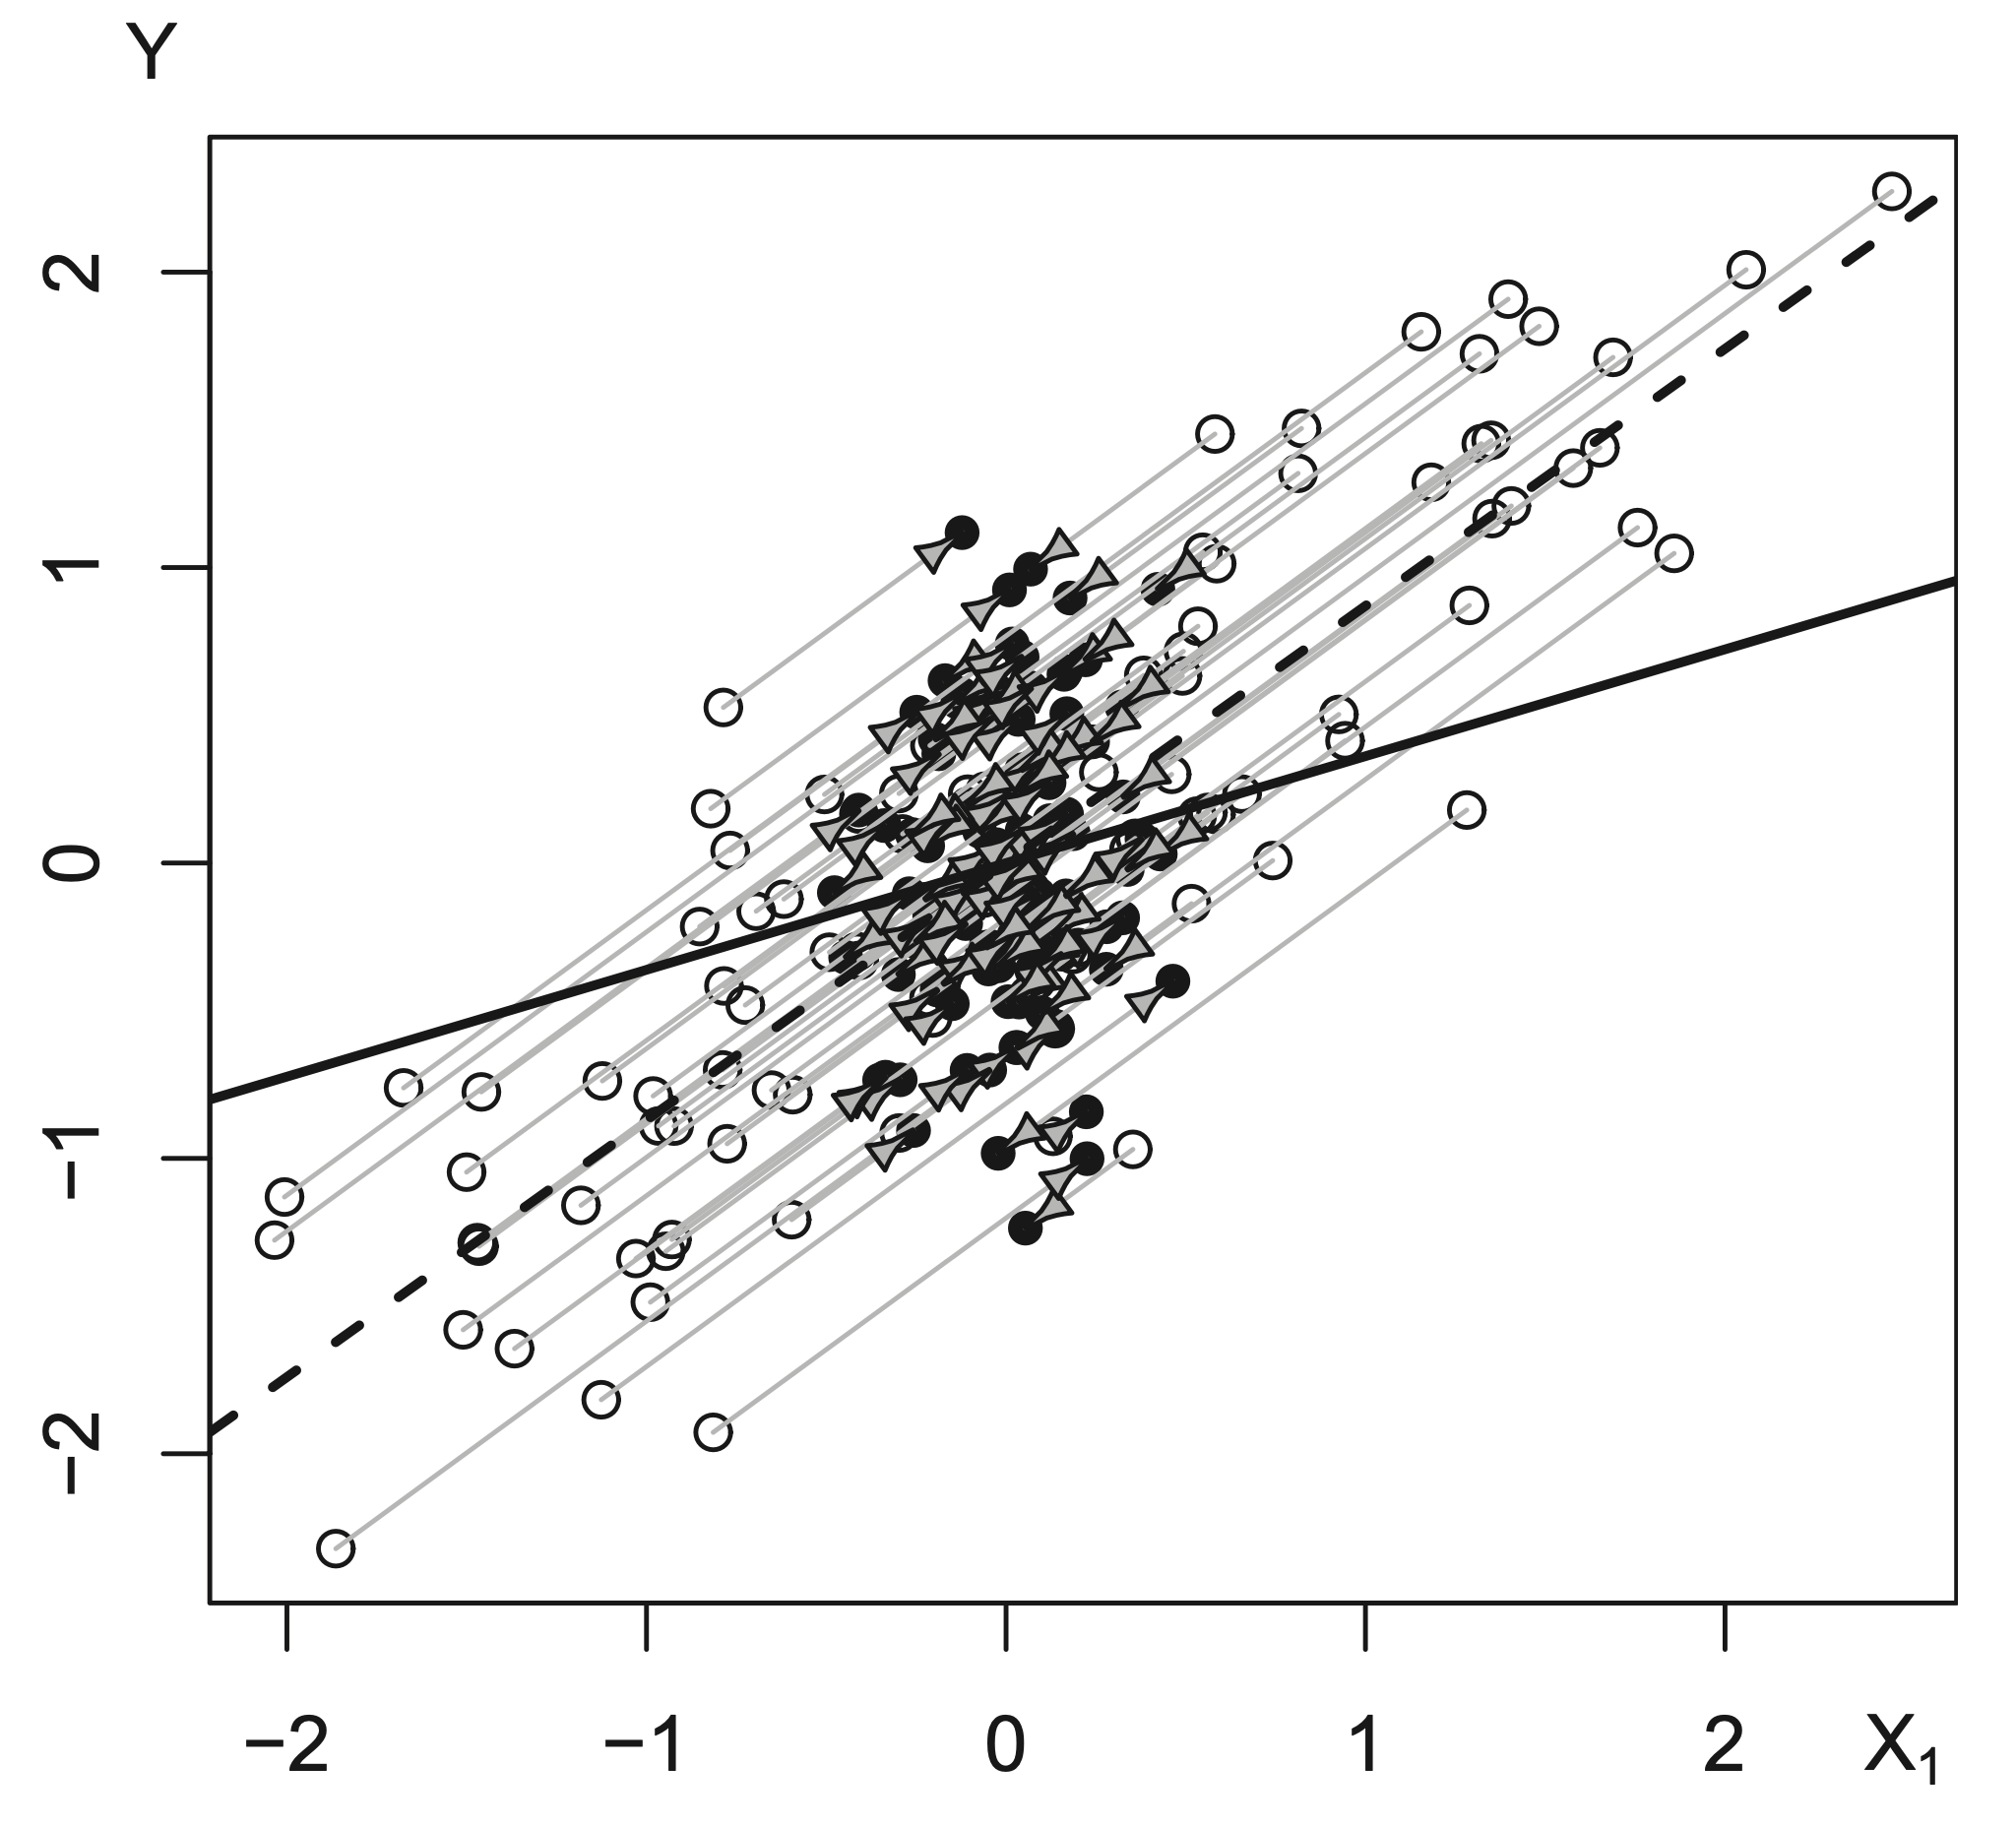
\includegraphics[width=0.9\textwidth]{Lecture17/JF_11_9}
  \caption{
  The marginal scatterplot (open circles) for $Y$ and $X_1$ superimposed on the added-variable plot (filled circles) for $X_1$ in the regression of $Y$ on $X_1$ and $X_2$.
  The variables $Y$ and $X_1$ are centered at their means to facilitate the comparison of the two sets of points.
  The arrows show how the points in the marginal scatterplot map into those in the AV plot.
  In this contrived data set, $X_1$ and $X_2$ are highly correlated ($r_{12} = 0.98$), and so the conditional variation in $X_1$ (represented by the horizontal spread of the filled points) is much less than its marginal variation (represented by the horizontal spread of the open points).
  The broken line gives the slope of the marginal regression of $Y$ on $X_1$ alone, while the solid line gives the slope $\hat{\beta}_1$ of $X_1$ in the MLR of $Y$ on both $X$s.
   JF Figure 11.9.}
  \label{fig:avp}
\end{center}
\end{figure}
%

Figure~\ref{fig:duncan_avp} illustrates the added-variable plots using the Duncan's data.
%
\begin{figure}[H]
\begin{center}
  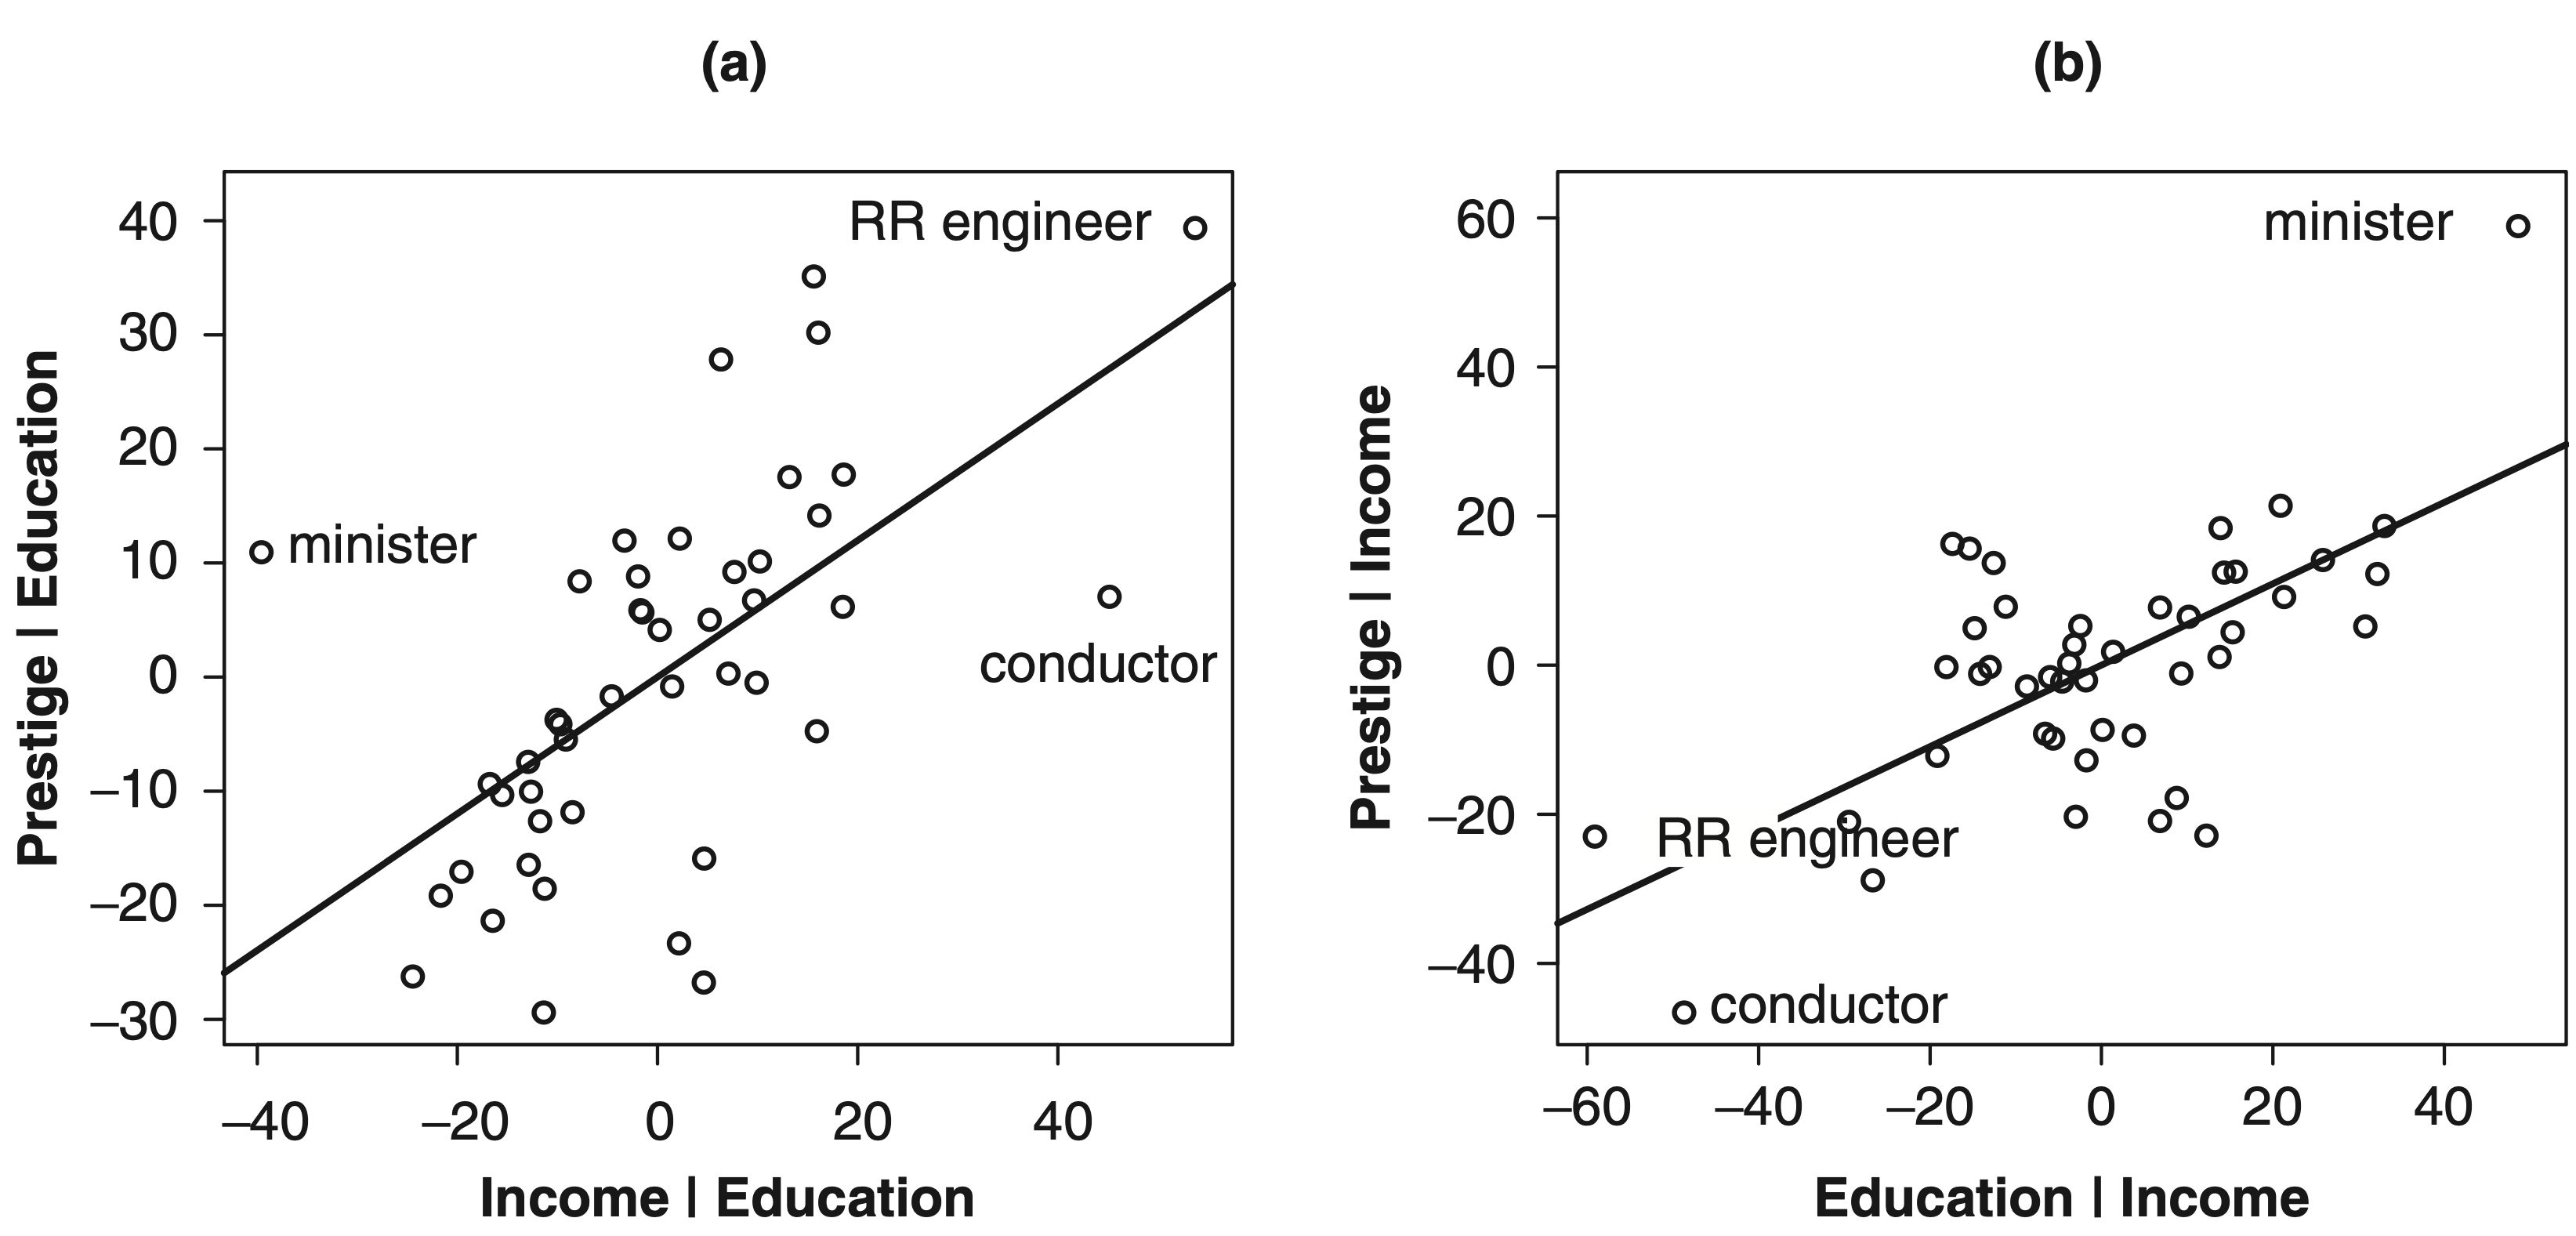
\includegraphics[width=0.9\textwidth]{Lecture17/JF_11_10}
  \caption{
  Added-variable plots for Duncan's regression of occupational prestige on the (a) income and (b) education levels of 45 US occupations in 1950.
  Three unusal observations, $miniters$, $conductors$, and $railroad engineers$, are identified on the plots.
  The added-variable plot for the intercept $\hat{\beta}_0$ is not shown.
   JF Figure 11.10.}
  \label{fig:duncan_avp}
\end{center}
\end{figure}
%

\subsection*{Should unusual data be discarded?}
In practice, although problematic data should not be ignored, they also should not be deleted automatically and without reflection:
\begin{itemize}
  \item It is important to investigate {\it why} an observation is unusual.  Truly ``bad'' data (e.g., an error in data entry ) can often be corrected or, if correction is not possible, thrown away.
  When a discrepant data point is correct, we may be able to understand why the observation is unusual.  
  For Duncan's data, for example, it makes sense that ministers enjoy prestige not accounted for by the income and educational levels of the occupation and for a reason not shared by other occupations.
  In a case like this, where an outlying observation has characteristics that render it unique, we may choose to set it aside from the rest of the data.
  \item Alternatively, outliers, high-leverage points, or influential data may motivate model respecification, and the pattern of unusual data may suggest the introduction of additional explanatory variables.
  We noticed, for example, that both conductors and railroad engineers had high leverage in Duncan's regression because these occupations combined relatively high income with relatively low education.
  Perhaps this combination of characteristics is due to a high level of unionization of these occupations in 1950, when the data were collected.
  If so, and if we can ascertain the levels of unionization of all of the occupations, we could enter this as an explanatory variable, perhaps shedding further light on the process determining occupational prestige.
  \item Except in clear-cut cases, we are justifiably reluctant to delete observations or to respecify the model to accommodate unusual data.
  Some researchers reasonably adopt alternative estimation strategies, such as robust regression, which continuously downweights outlying data rather than simply discarding them.
  Because these methods assign zero or very small weight to highly discrepant data, however, the result is generally not very different from careful application of least squares, and , indeed, robust-regression weights can be used to identify outliers.
  \item Finally, in large samples, unusual data substantially alter the results only in extreme instances.
  Identifying unusual observations in a large sample, therefore, should be regarded more as an opportunity to learn something about the data not captured by the model that we have fit, rather than as an occasion to reestimate the model with the unusual observations removed.
  
\end{itemize}




\newpage
\setcounter{section}{17}


\section{Lecture 18: March 1}


\subsection*{Last time}
\begin{itemize}
 \item Unusual and influential data (JF chapter 11)
\end{itemize}


\subsection*{Today}
\begin{itemize}
 \item HW2 deadline extends to end of this week.
 \item Diagnosing non-normality, non-constant error variance, and nonlinearity (JF chapter 12)
 \item Data transformation (JF chapter 4)
\end{itemize}


\subsubsection*{Central Limit Theorem}
Let $X_1, X_2, \dots$ be a sequence of iid random variables whose mgfs exist in a neighborhood of $0$ (that is, $M_{X_i}(t)$ exists for $|t| < h$, for some positive $h$).
Let $\mbox{E}{X_i}=\mu$ and $\sVar{X_i}=\sigma^2 >0$. (Both $\mu$ and $\sigma^2$ are finite since the mgf exists.). Define $\bar{X}_n = (1/n)\sum\limits_{i = 1}^n X_i$.
Let $G_n(x)$ denote the cdf of $\sqrt{n} (\bar{X}_n - \mu)/\sigma$.
Then, for any $x$, $-\infty < x < \infty$,
$$
\lim\limits_{n \to \infty} G_n(x) = \int_{-\infty}^x \frac{1}{\sqrt{2\pi}} e^{-y^2/2}dy
$$
that is, $\sqrt{n}(\bar{X}_n - \mu)/\sigma$ has a limiting standard normal distribution.
(Refer to Casella \& Berger p.237 - p.238 for a proof.)

\subsubsection*{Delta Method}
Let $Y_n$ be a sequence of random variables that satisfies $\sqrt{n} (Y_n - \theta) \to N(0, \sigma^2)$ in distribution.
For a given function $g$ and a specific value of $\theta$, suppose $g'(\theta)$ exists and is not $0$.  Then
$$
\sqrt{n} [ g(Y_n) - g(\theta) ] \to N(0, \sigma^2 [g'(\theta)]^2) \mbox{ in distribution}.
$$
(Refer to Casella \& Berger p.243 for a proof using Taylor expansion.)

\subsubsection*{Second-order Delta Method}
Let $Y_n$ be a sequence of random variables that satisfies $\sqrt{n} (Y_n - \theta) \to N(0, \sigma^2)$ in distribution.
For a given function $g$ and a specific value of $\theta$, suppose that $g'(\theta)=0$ and $g''(\theta)$ exists and is not $0$.  Then
$$
\sqrt{n} [ g(Y_n) - g(\theta) ] \to \sigma^2 \frac{g''(\theta)}{2} \chi_1^2  \mbox{ in distribution}.
$$

\subsection*{Non-normally distributed errors}

The assumption of normally distributed errors is almost always arbitrary.  
Nevertheless, the central limit theorem ensures that, under very broad conditions, inference based on the least-squares estimator is approximately valid in all but small samples.
Why concern about non-normal errors?
\begin{itemize}
  \item For some types of error distributions, particularly those with heavy tails, the efficiency of least-squares estimation decreases markedly.
  \item Highly skewed error distributions, aside from their propensity to generate outliers in the direction of the skew, compromise the interpretation of the least-squares fit.
  This fit is a conditional mean (of $Y$ given the $X$s), and the mean is not a good measure of the center of a highly skewed distribution.
  \item A multimodal error distribution suggests that omission of one or more discrete explanatory variables that divide the data naturally into groups.  
  An examination of the distribution of the residuals may motivate respecification of the model.
\end{itemize}

Note: The \underline{skewness $\alpha_3$} is defined as $\alpha_3 \equiv \frac{\mu_3}{(\mu_2)^{3/2}}$ where $\mu_n$ denotes the $n$th central moment of a random variable $X$.
The skewness measures the lack of symmetry in the pdf.

\subsubsection*{Quantile-comparison plot, JF 3.1.3}
{\it Quantile-comparison plots} are useful for comparing an empirical sample distribution with a theoretical distribution, such as the normal distribution.

Let $P(x)$ represent the theoretical cumulative distribution function (cdf) with which we want to compare the data, that is $P(x) = \Pr(X \le x)$.
The quantile-comparison plot is constructed by:
\begin{enumerate}
  \item Order the data values from smallest to largest, $X_{(1)}, X_{(2)}, \dots, X_{(n)}$.  The $X_{(i)}$ are called the \underline{order statistics} of the sample.
  \item By convention, the cumulative proportion of the data ``below'' $X_{(i)}$ is given by 
  $$
  P_i = \frac{i - \frac{1}{2}}{n}
  $$
  \item  Use the inverse of the cdf to find the value $z_i$ corresponding to the cumulative probability $P_i$, that is
  $$
  z_i = P^{-1}(\frac{i - \frac{1}{2}}{n})
  $$
  \item Plot the $z_i$ as horizontal coordinates against the $X_{(i)}$ as vertical coordinates.  If $X$ is sampled from the distribution $P$, then $X_{(i)}\approx z_i$.
  \begin{itemize}
    \item if the distributions are identical except for location, then the plot is approximately linear with nonzero intercept, $X_{(i)} \approx \mu + z_i$
    \item if the distributions are identical except for scale, then the plot is approximately linear with a slope different from $1$, $X_{(i)} \approx \sigma z_i$
    \item if the distributions differ both in location and scale but have the same shape, then $X_{(i)} \approx \mu + \sigma z_i$
  \end{itemize}
  \item It is often helpful to place a comparison line on the plot to facilitate the perception of departures from linearity.  
  For a normal quantile-comparison plot (comparing the distribution of the data with the standard normal distribution), we can alternatively use the median as a robust estimator of $\mu$ and the interquartile range/1.39 as a robust estimator of $\sigma$.
  \item We expect some departure from linearity because of sampling variation.
  It therefore assists interpretation to display the expected degree of sampling error in the plot.
  The standard error of the order statistic $X_{(i)}$ is 
  $$
  \mbox{SE}(X_{(i)}) = \frac{\hat{\sigma}}{p(z_i)} \sqrt{\frac{P_i(1 - P_i)}{n}}
  $$
  where $p(z_i)$ is the probability density function, pdf, corresponding to the CDF $P(z)$.
  The values along the fitted line are given by $\hat{X}_{(i)} = \hat{\mu} + \hat{\sigma}z_i$.
  An approximate 95\% confidence ``envelope'' around the fitted line is, therefore,
  $$
  \hat{X}_{(i)} \pm 2\times \mbox{SE}(X_{(i)}) 
  $$
\end{enumerate}

\begin{itemize}
  \item Figure~\ref{fig:JF_3_8} plots a sample of $n=100$ observations from a normal distribution with mean $\mu = 50$ and standard deviation $\sigma = 10$.
%
\begin{figure}[H]
	\begin{center}
		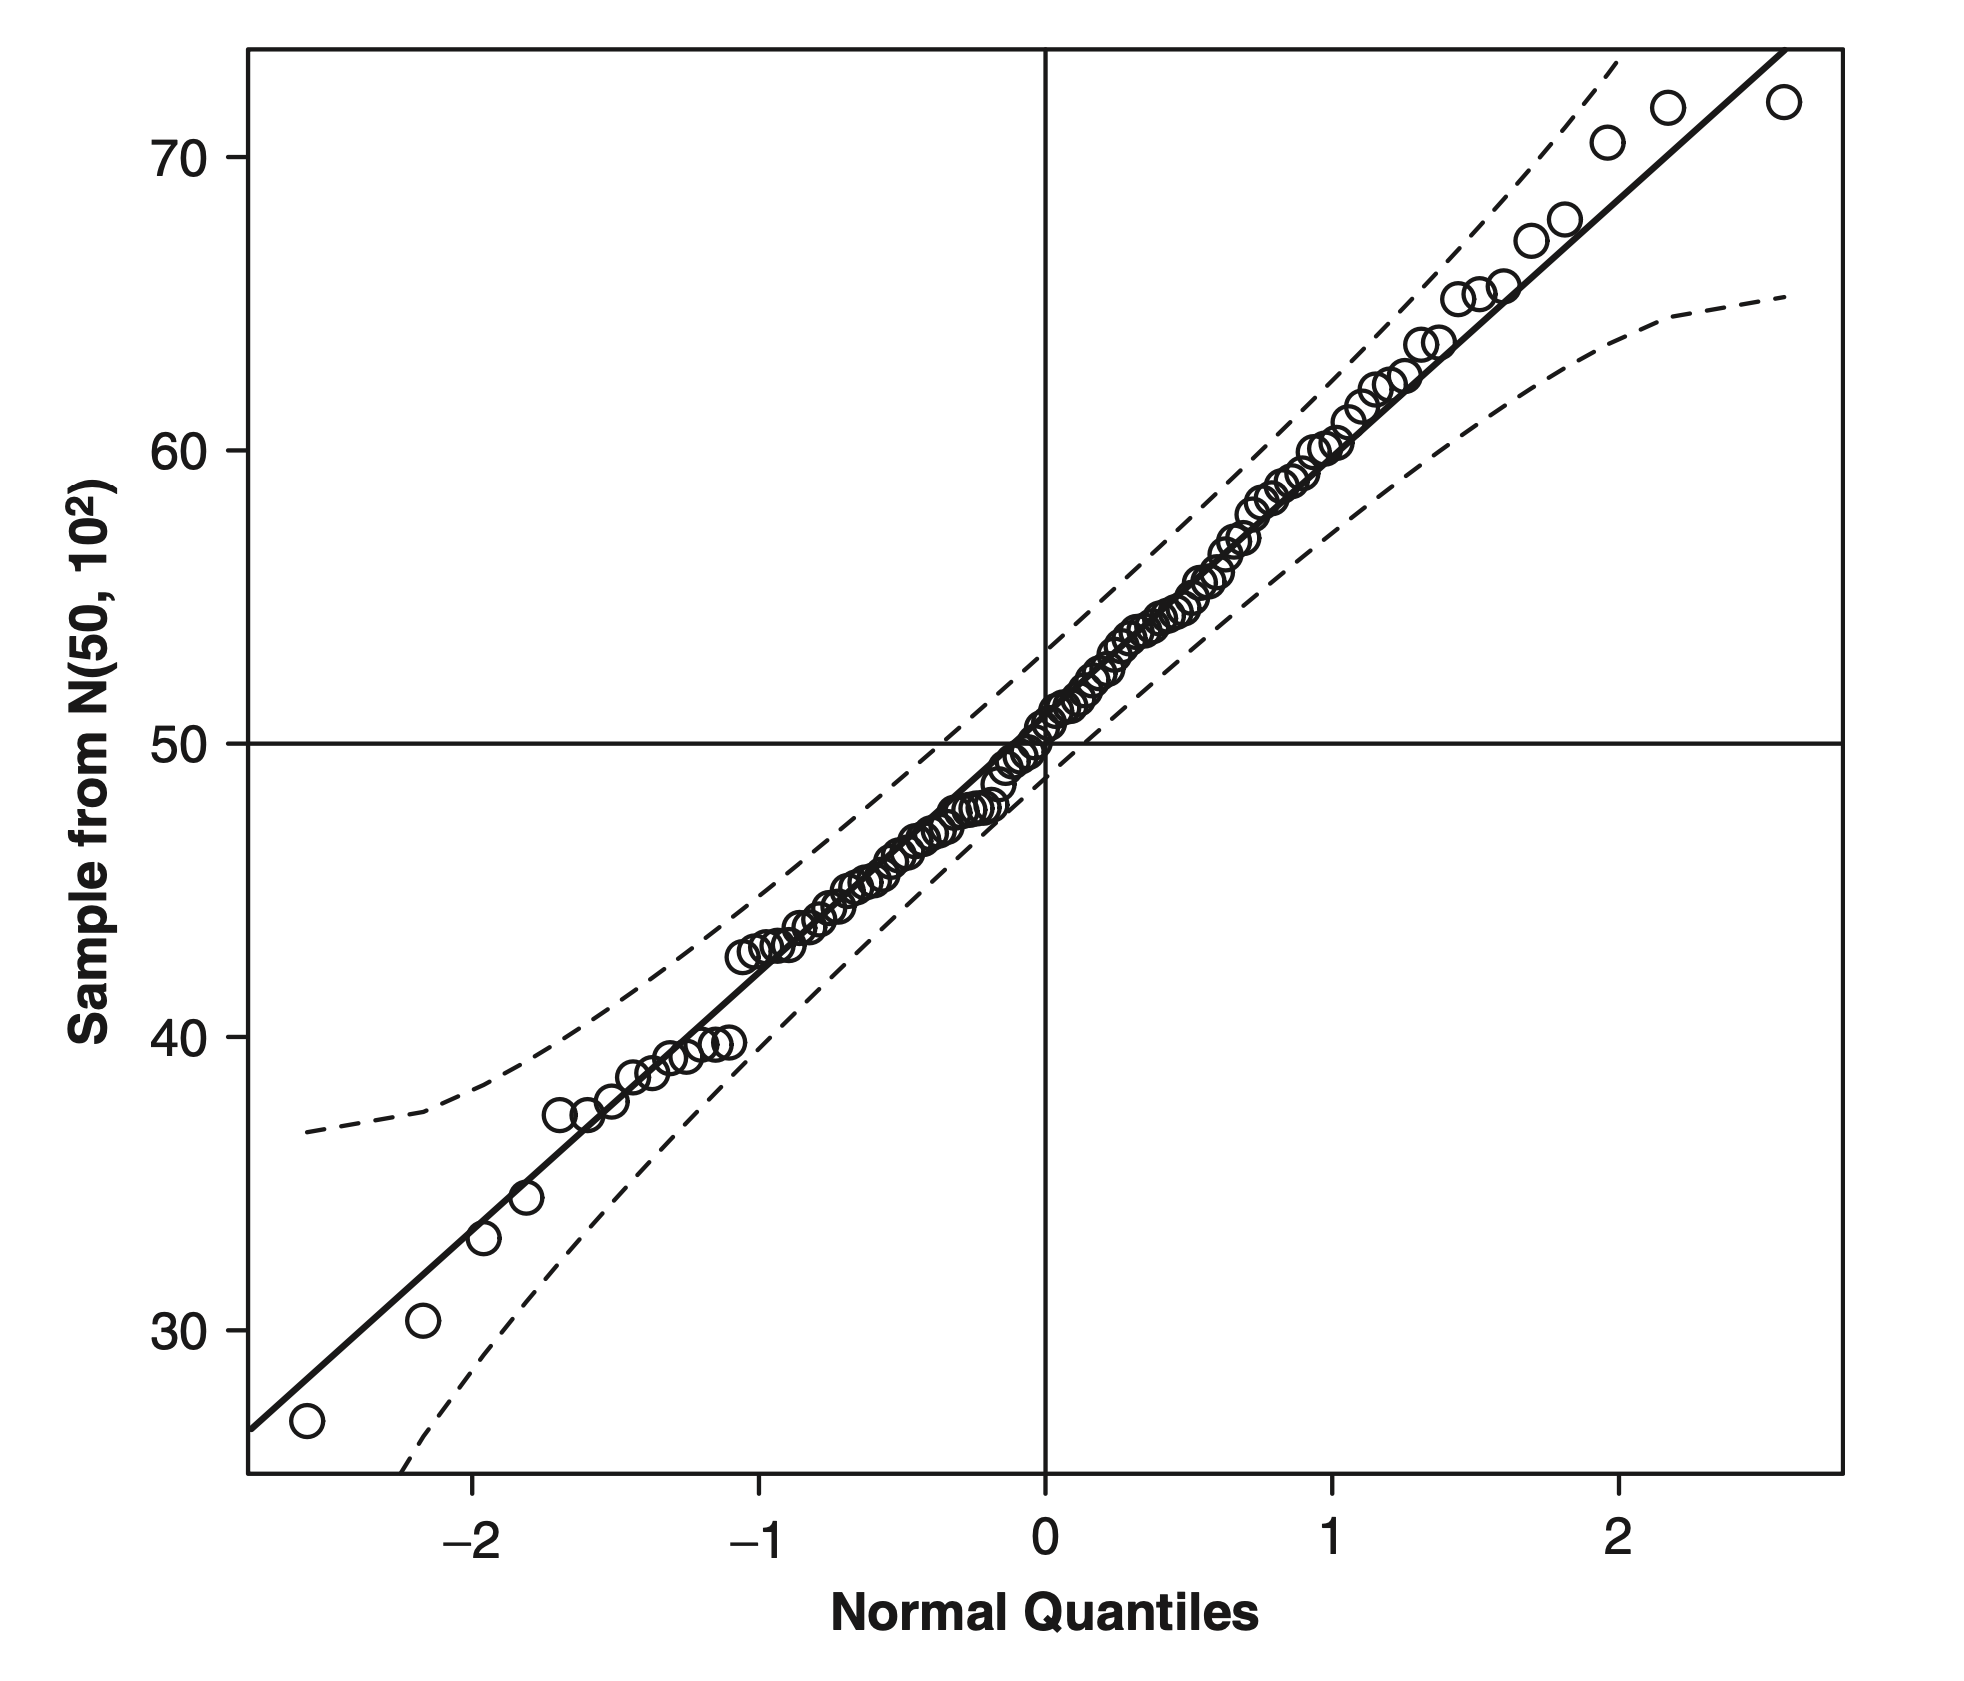
\includegraphics[width=0.8\textwidth]{Lecture18/JF_3_8}
		\caption{
			Normal quantile-comparison plot for a sample of $100$ observations drawn from a normal distribution with mean $50$ and standard deviation $10$.
			The fitted line is through the quartiles of the distribution, the broken lines give a pointwise 95\% confidence interval around the fit.
			JF Figure 3.8.}
		\label{fig:JF_3_8}
	\end{center}
\end{figure}
%  
  The plotted points are reasonably linear and stay within the rough 95\% confidence envelope.
  \item Figure~\ref{fig:JF_3_9} plots a sample of $n=100$ observations from the positively skewed chi-square distribution with 2 degrees of freedom.
  The positive skew of the data is reflected in points that lie {\it above} the comparison line in both tails of the distribution. (In contrast, the tails of negatively skewed data would lie {\it below} the comparison line.)
%
\begin{figure}[H]
	\begin{center}
		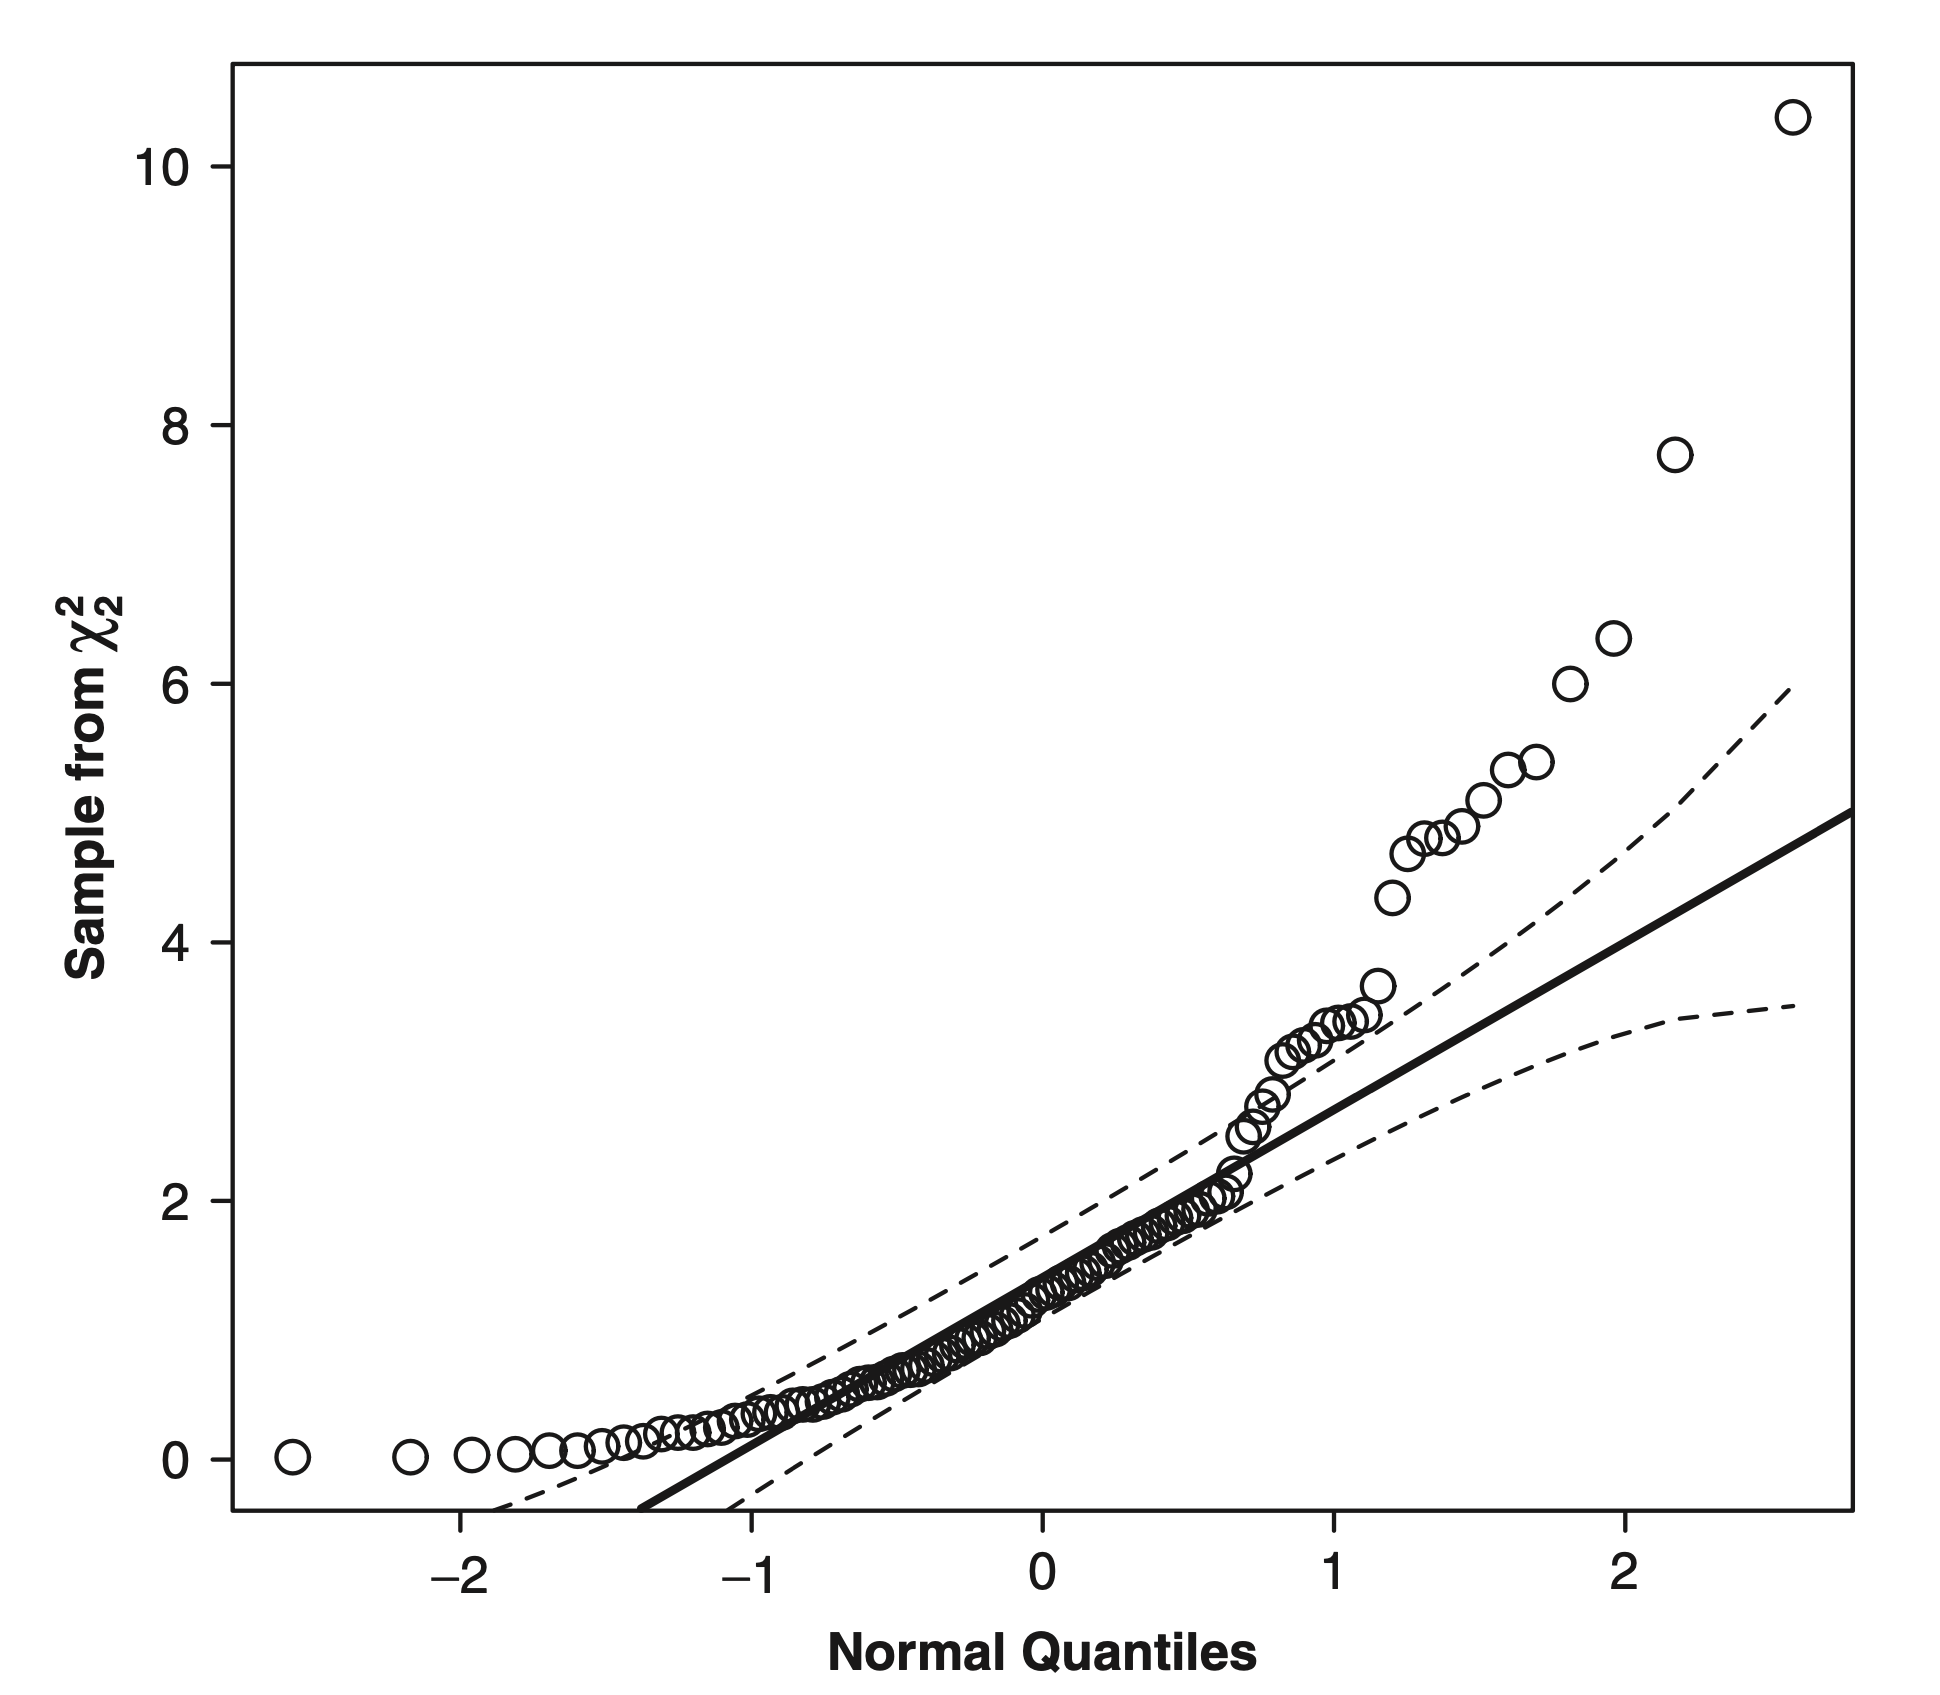
\includegraphics[width=0.8\textwidth]{Lecture18/JF_3_9}
		\caption{
			Normal quantile-comparison plot for a sample of $100$ observations drawn from the positively skewed chi-square distribution with 2 degrees of freedom.
			JF Figure 3.9.}
		\label{fig:JF_3_9}
	\end{center}
\end{figure}
%  
  \item Figure~\ref{fig:JF_3_10} plots a sample of $n = 100$ observations from the heavy-tailed $t$ distribution with 2 degrees of freedom.
  In this case, values in the upper tail lie above the corresponding normal quantiles, the values in the lower tail below the corresponding normal quantiles.
%
\begin{figure}[H]
	\begin{center}
		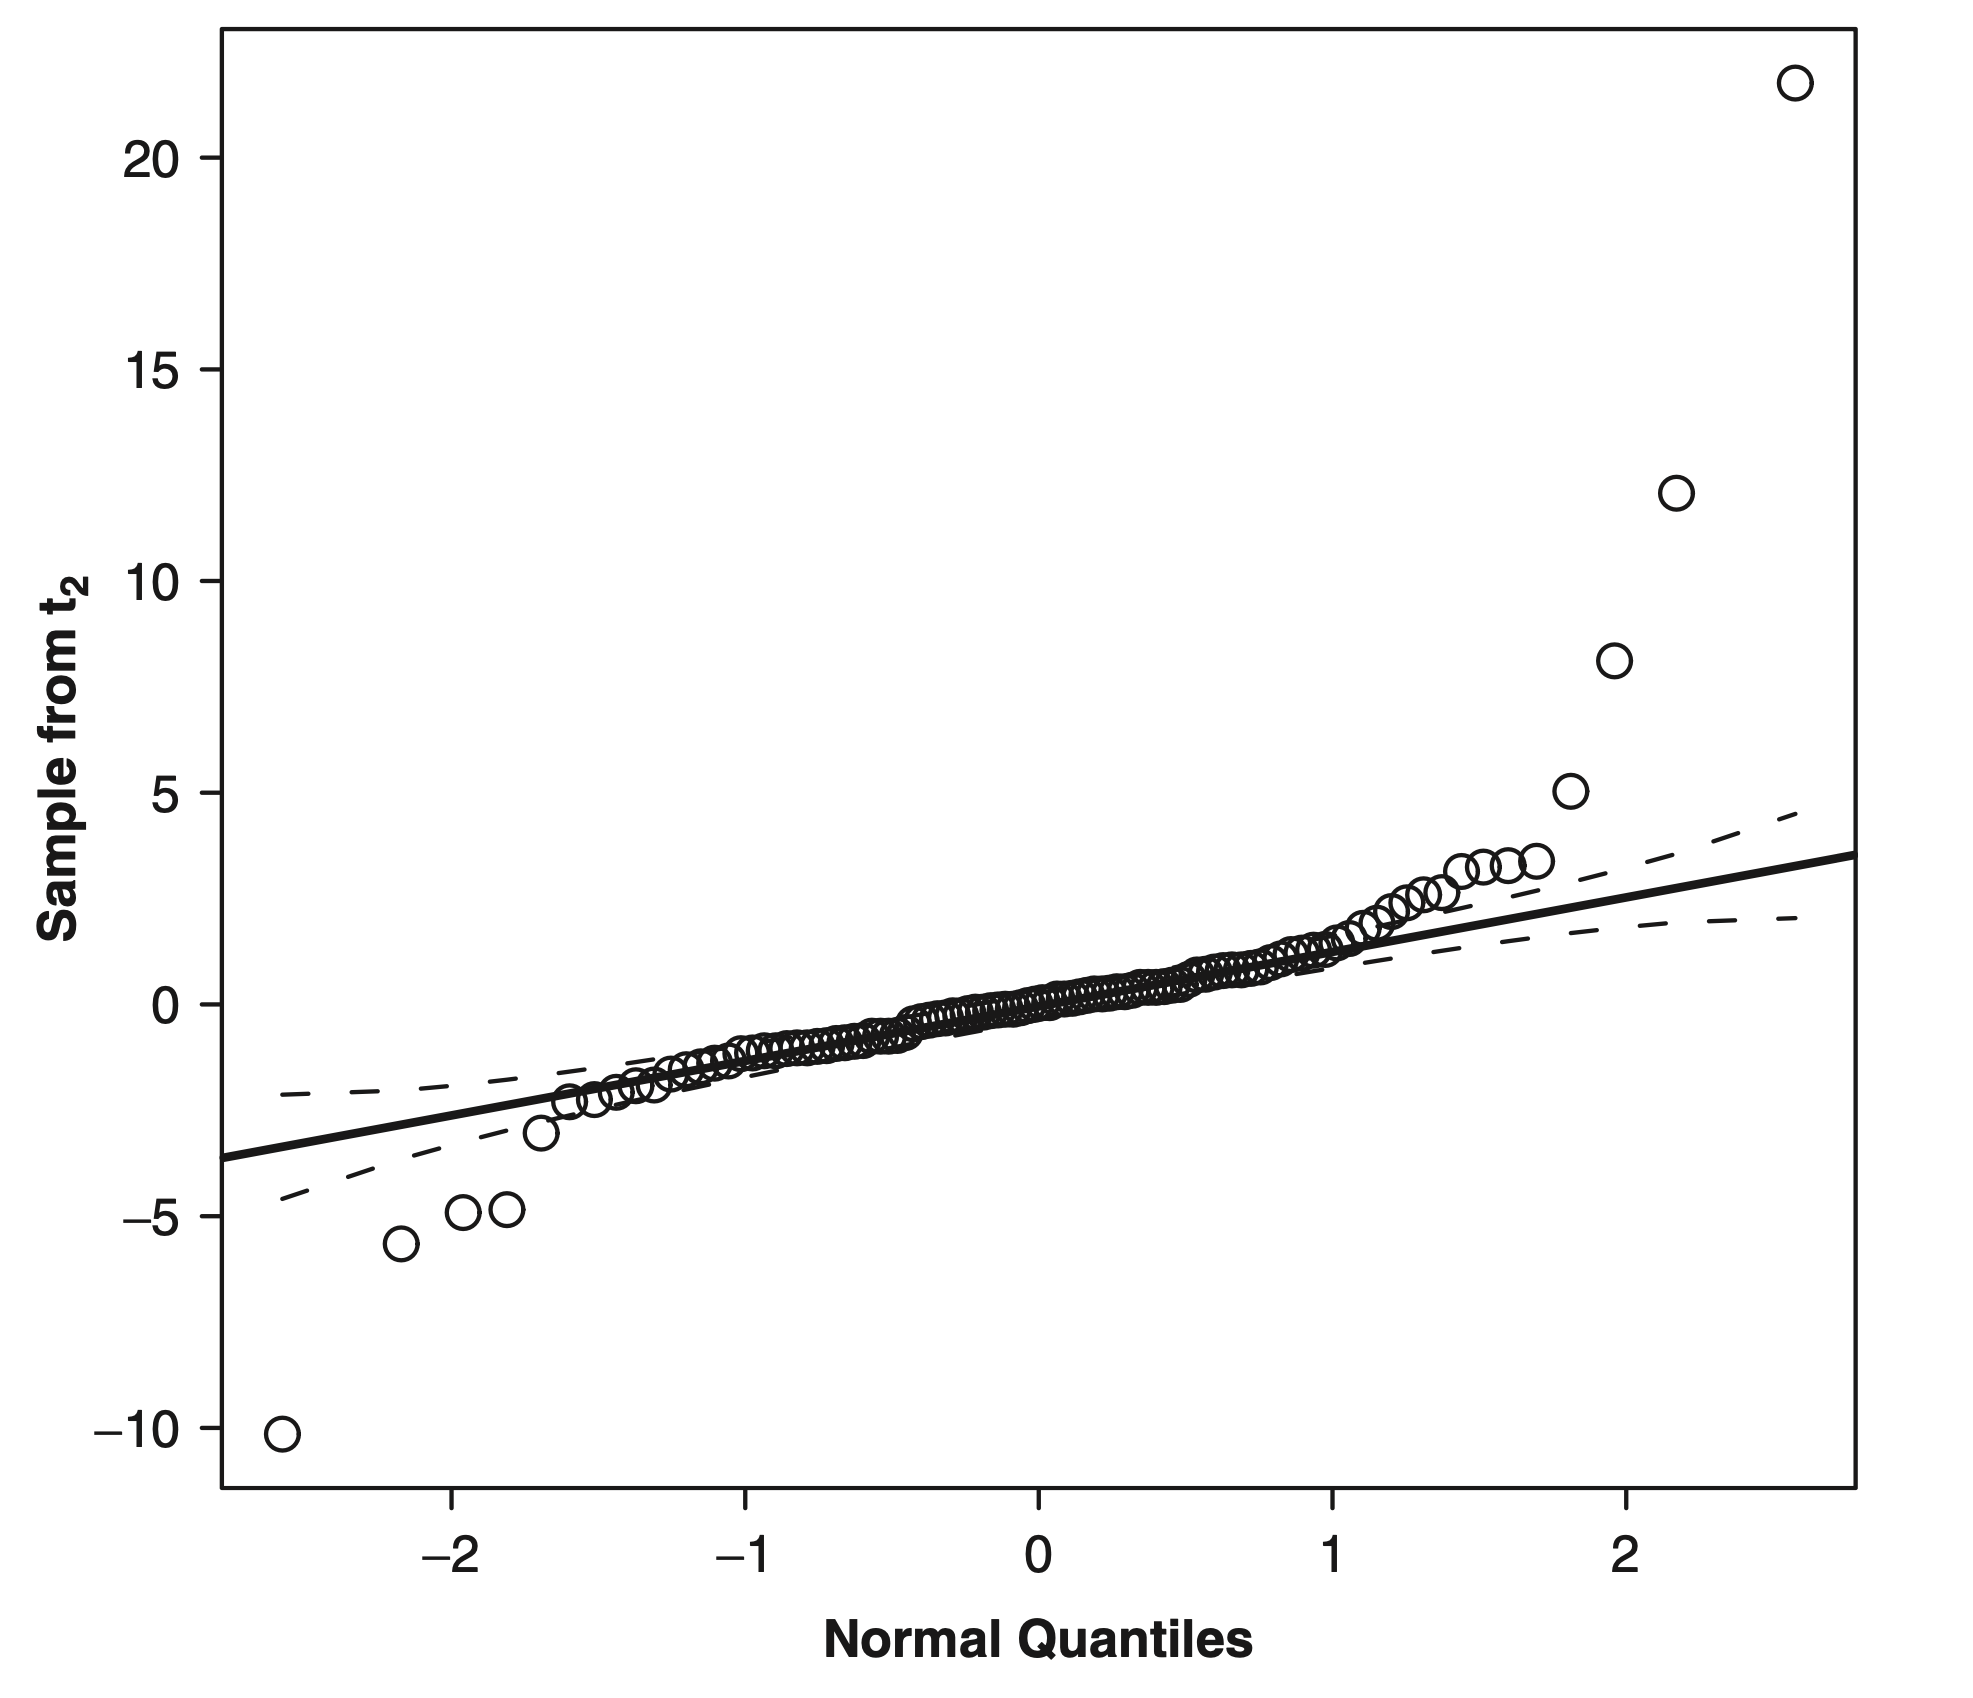
\includegraphics[width=0.8\textwidth]{Lecture18/JF_3_10}
		\caption{
			Normal quantile-comparison plot for a sample of $100$ observations drawn from heavy-tailed $t$-distribution with 2 degrees of freedom.
			JF Figure 3.10.}
		\label{fig:JF_3_10}
	\end{center}
\end{figure}
%  
  \item Figure~\ref{fig:JF_3_11} shows the normal quantile-comparison plot for the distribution of infant mortality.  The positive skew of the distribution is readily apparent.
%
\begin{figure}[H]
	\begin{center}
		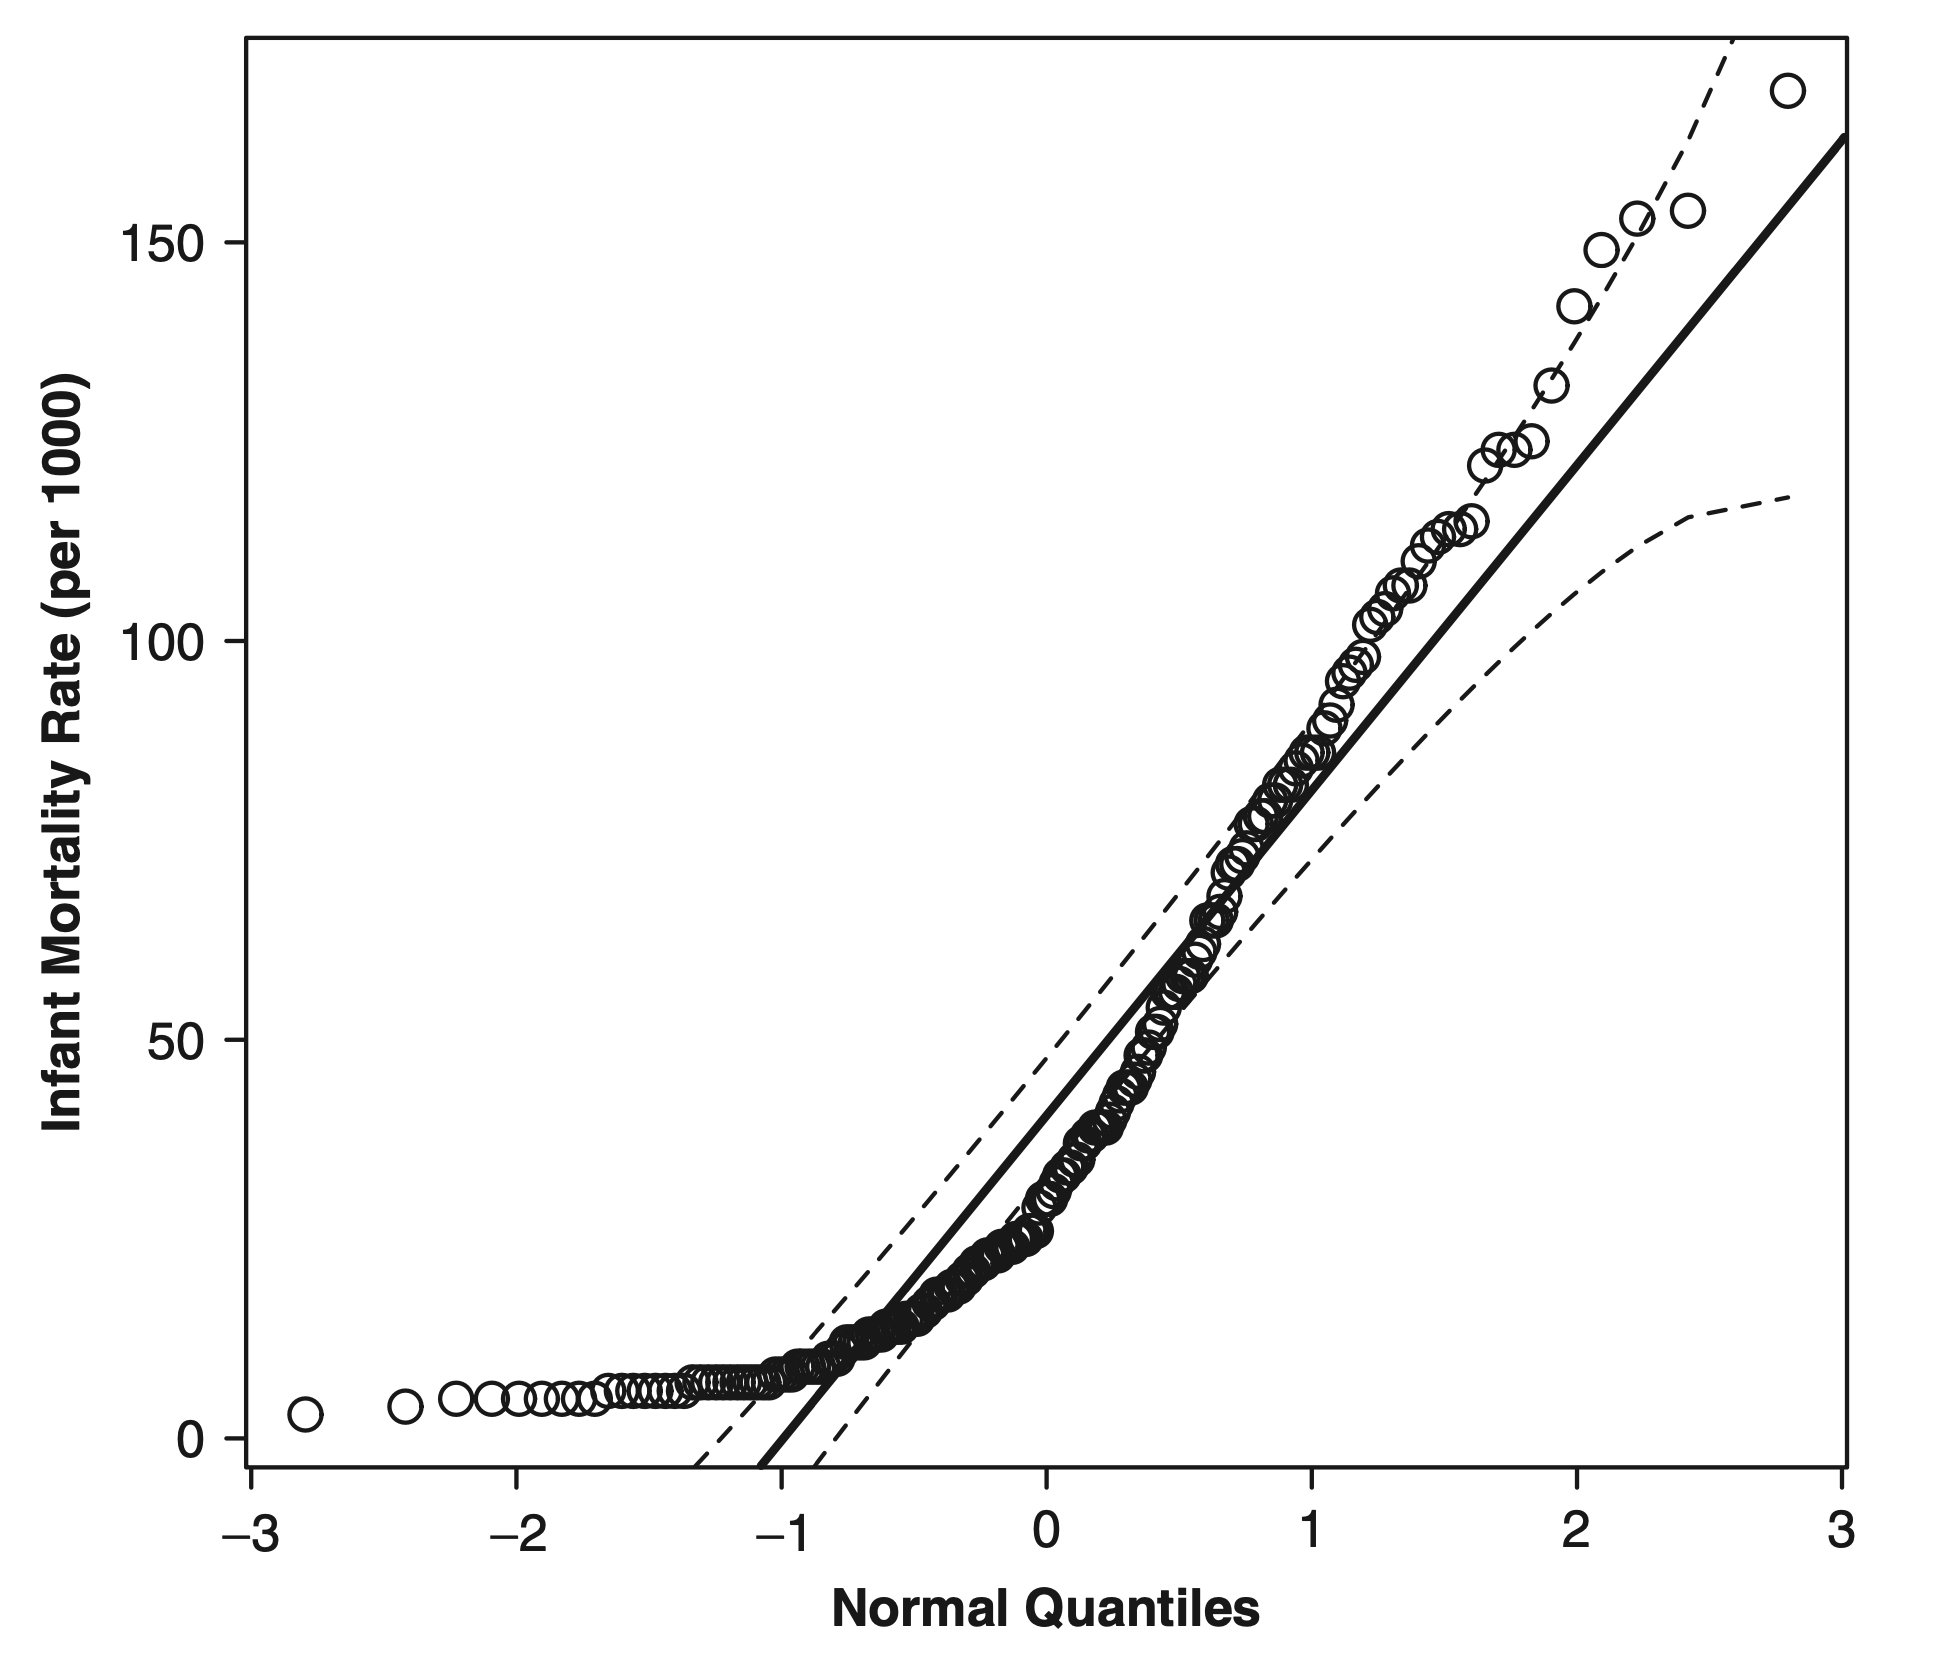
\includegraphics[width=0.8\textwidth]{Lecture18/JF_3_11}
		\caption{
			Normal quantile-comparison plot for the distribution of infant mortality.  Note the positive skew.
			JF Figure 3.11.}
		\label{fig:JF_3_11}
	\end{center}
\end{figure}
%  
\end{itemize}




\subsection*{Nonconstant error variance}
One of the assumptions of the regression model is that the variation of the response variable around the regression surface (the error variance) is everywhere the same:
$$
\sVar(\epsilon) = \sVar(Y | x_1, \dots, x_p) = \sigma_\epsilon^2
$$

Constant error variance is often termed \underline{homoscedasticity}, and similarly, nonconstant error variance is termed \underline{heteroscedasticity}.
We detect nonconstant error variances through graphical methods.

\subsubsection*{Residual plots}
Because the least square residuals have unequal variance even when the constant variance assumption is correct:
$$
\sVar(\hat{\epsilon}_i) = \sigma^2 (1 - h_i).
$$
It is preferable to plot studentized residuals against fitted values.
A pattern of changing spread is often more easily discerned in a plot of absolute studentized residuals, $|\hat{\epsilon}_i^{*}|$, or squared studentized residuals, $\hat{\epsilon}_i^{*2}$, against $\hat{Y}$.
If the values of $\hat{Y}$ are all positive, then we can plot $\log |\hat{\epsilon}_i^{*}|$ against $\log \hat{Y}$.
Figure~\ref{fig:JF_12_3} shows a plot of studentized residuals against fitted values and spread-level plot of studentized residuals, several points with negative fitted values were omitted.
%
\begin{figure}[H]
\begin{center}
  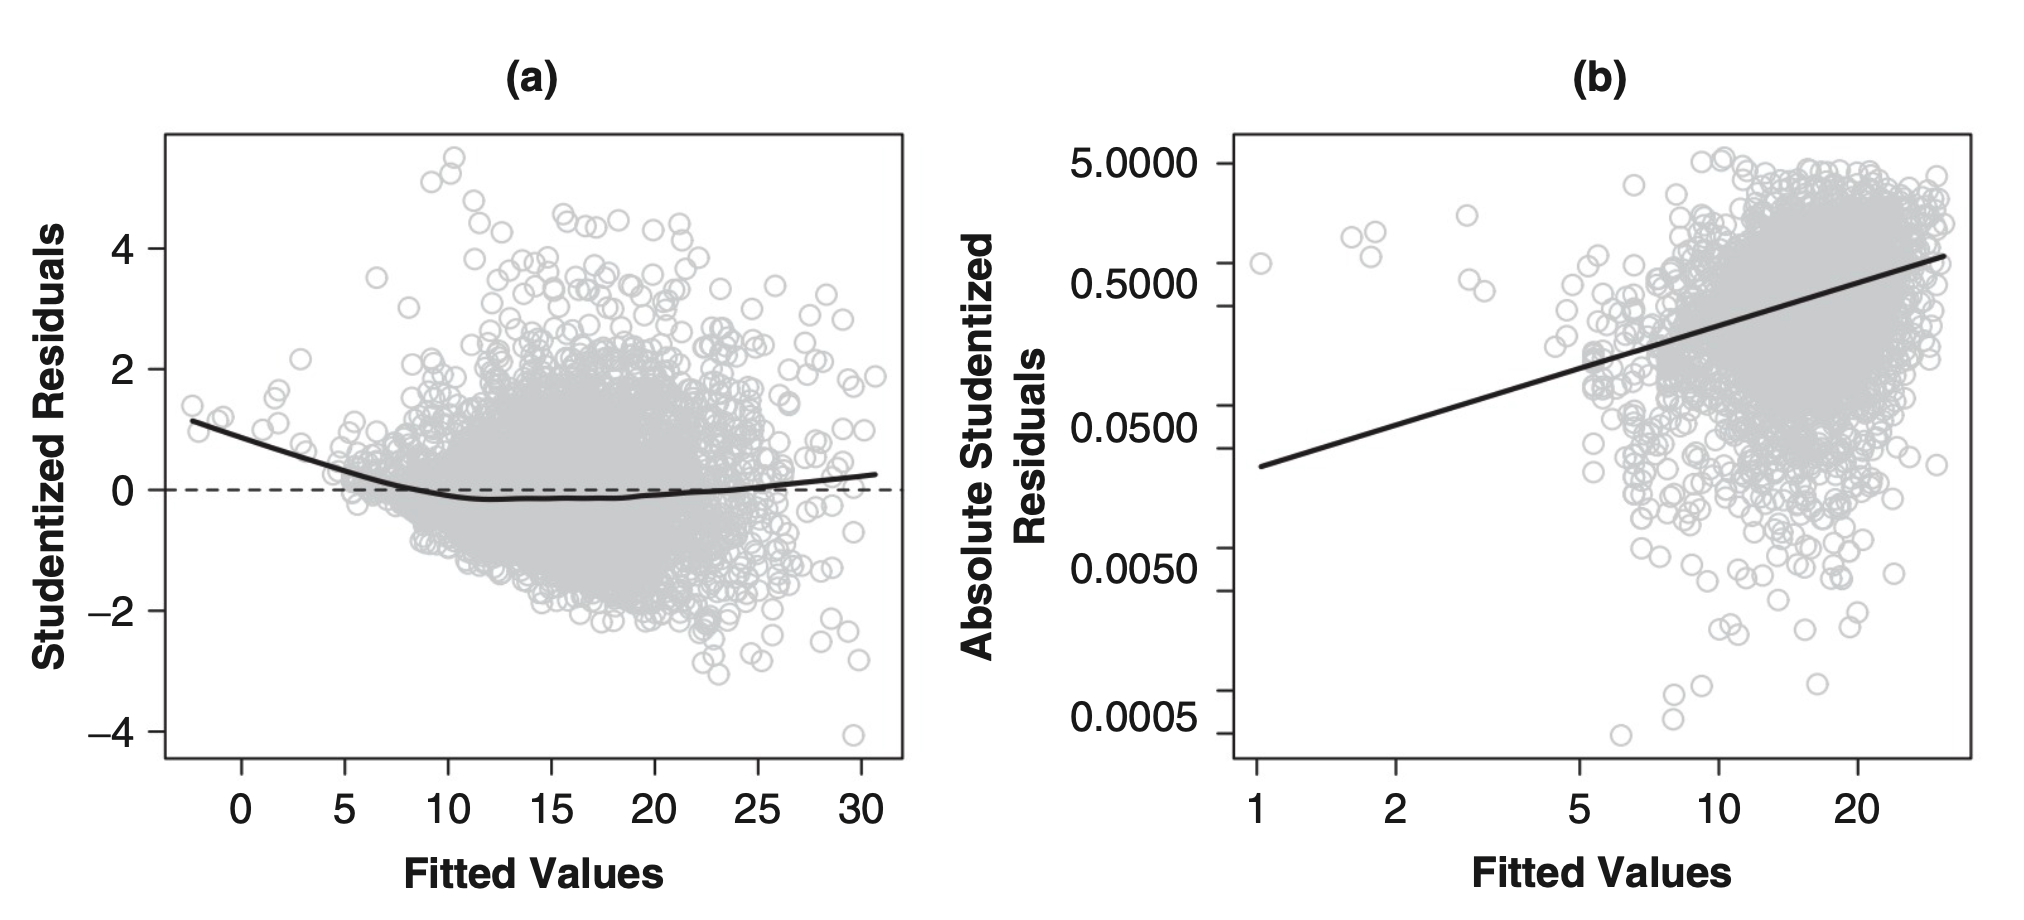
\includegraphics[width=0.9\textwidth]{Lecture18/JF_12_3}
  \caption{(a) Plot of studentized residuals versus fitted values and (b) spread-level plot for studentized residuals.
   JF Figure 12.3.}
  \label{fig:JF_12_3}
\end{center}
\end{figure}
%
It is apparent from both graphs that the residual spread tends to increase with the level of the response, suggesting a violation of constant error variance assumption.

\subsubsection*{Weighted-least-squares estimation}

\underline{Weighted-least-squares} (WLS) regression provides an alternative approach to estimation in the presence of nonconstant error variance.
Suppose that the errors from the linear regression model $\vecc{Y} = \vecc{X\beta} + \vecc{\epsilon}$ are independent and normally distributed, with zero means but {\it different} variances:
$\epsilon_i \sim N(0, \sigma^2_i)$.
Suppose further that the variances of the errors are known up to a constant of proportionality $\sigma_\epsilon^2$, so that $\sigma_i^2 = \sigma_\epsilon^2/w_i^2$.
Then the likelihood for the model is
$$
L(\beta, \sigma_\epsilon^2) = \frac{1}{(2\pi)^{n/2} |\vecc{\Sigma|}^{1/2}}\exp\left[ -\frac{1}{2}(\vecc{Y} - \vecc{X\beta})\transpose \vecc{\Sigma}^{-1} (\vecc{Y} - \vecc{X\beta}) \right]
$$
where $\vecc{\Sigma}$ is the covariance matrix of the errors,
$$
\vecc{\Sigma} = \sigma_\epsilon^2 \times \mbox{diag}\{1/w_1^2, \dots, 1/w_n^2\} \equiv \sigma_\epsilon^2 \vecc{W}^{-1}
$$
The maximum-likelihood estimators of $\vecc{\beta}$ and $\sigma_\epsilon^2$ are then
$$
\begin{aligned}
\hat{\vecc{\beta}} &= (\vecc{X}\transpose \vecc{WX}) ^ {-1} \vecc{X}\transpose \vecc{WY}\\
\hat{\sigma}_\epsilon^2 &= \frac{\sum(w_i\hat{\epsilon}_i)^2}{n}\\
\end{aligned}
$$

\subsubsection*{Correcting OLS standard errors for nonconstant variance}
The covariance matrix of the \underline{ordinary-least-squares} (OLS) estimator is
$$
\begin{aligned}
\Var{\hat{\beta}} &= (\vecc{X}\transpose \vecc{X})^{-1} \vecc{X}\transpose \Var{\vecc{Y}} \vecc{X} (\vecc{X}\transpose \vecc{X})^{-1}\\
&= \sigma_\epsilon^2  (\vecc{X}\transpose \vecc{X})^{-1} \\
\end{aligned}
$$
under the standard assumptions, including the assumption of constant error variance, $\Var{\vecc{Y}} = \sigma_\epsilon^2\vecc{I}_n$.
If, however, the errors are heteroscedastic but independent then $\vecc{\Sigma} \equiv \Var{\vecc{Y}} = \mbox{diag}\{\sigma_1^2, \dots, \sigma_n^2 \}$, and 
$$
\Var{\hat{\beta}} = (\vecc{X}\transpose \vecc{X})^{-1} \vecc{X}\transpose \vecc{\Sigma} \vecc{X} (\vecc{X}\transpose \vecc{X})^{-1}
$$
White (1980) shows that the following is a consistent estimator of $\Var{\hat{\beta}}$
$$
\tilde{\sVar}(\hat{\vecc{\beta}}) = (\vecc{X}\transpose \vecc{X})^{-1} \vecc{X}\transpose \hat{\vecc{\Sigma}} \vecc{X} (\vecc{X}\transpose \vecc{X})^{-1}
$$
with $\hat{\vecc{\Sigma}} = \mbox{diag}\{\hat{\sigma}_1^2, \dots, \hat{\sigma}_n^2\}$, where $\hat{\sigma}_i^2$ is the OLS residual for observation $i$.

Subsequent work suggested small modifications to White's coefficient-variance estimator, and in particular simulation studies by Long and Ervin (2000) support the use of 
$$
\tilde{\sVar}^*(\hat{\vecc{\beta}}) = (\vecc{X}\transpose \vecc{X})^{-1} \vecc{X}\transpose \hat{\vecc{\Sigma}}^* \vecc{X} (\vecc{X}\transpose \vecc{X})^{-1}
$$
where $\hat{\vecc{\Sigma}}^* = \mbox{diag}\{\hat{\sigma}_i^2/(1 - h_i)^2\}$ and $h_i$ is the hat-value associated with observation $i$.
In large samples, where $h_i$ is small, the distinction between $\tilde{\sVar}(\hat{\vecc{\beta}})$ and $\tilde{\sVar}^*(\hat{\vecc{\beta}})$ essentially disappears.

A rough {\it rule} is that nonconstant error variance seriouly degrades the least-squares estimator only when the ratio of the largest to smallest variance is about $10$ or more (or, more conservatively, about $4$ or more).




%
%
%\subsection*{Polynomial regression}




















\newpage
\setcounter{section}{18}


\section{Lecture 19: March 3}


\subsection*{Last time}
\begin{itemize}
  \item Diagnosing non-normality, non-constant error variance (JF chapter 12)
\end{itemize}


\subsection*{Today}
\begin{itemize}
\item Diagnosing nonlinearity (JF chapter 12)
\item Data transformation (JF chapter 4)
\end{itemize}

\subsection*{Nonlinearity}

If $\Expected{\vecc{Y}|\vecc{X}}$ is not linear in $\vecc{X}$ (in other words, $\Expected{\vecc{\epsilon} | \vecc{X}} \ne 0$ for some $x$), $\hat{\vecc{\beta}}$ may be biased and inconsistent.
Usually we employ ``linearity by default'' but we should try to make sure this is appropriate: {\bf detect} non-linearities and {\bf model} them accurately.

\subsubsection*{Lowess smoother, JF 2.3}
We can employ local averaging plots to help with diagnostics.
\underline{Lowess} method is in many respects similar to local-averaging smoothers, except that instead of computing an average $Y$-value within the neighborhood of a focal $x$,
the lowess smoother computes a {\it fitted} value based on a locally weighted least-squares line, giving more weight to observations in the neighborhood that are close to the focal $x$ than
to those relatively far away.
The name ``lowess'' is an acronym for {\it lo}cally {\it we}ighted {\it s}catterplot {\it s}moother and is sometimes rendered as {\it loess}, for {\it lo}cal regr{\it ess}ion. 
 (If time permitted, we will revisit local regression in Nonparametric Regression.)

\subsubsection*{Component-plus-residual plots}
Component-plut-residual plots are constructed by
\begin{enumerate}
  \item Compute residuals from full regression:
  $$
  \hat{\epsilon_i} = Y_i - \hat{Y}_i
  $$
  \item Compute ``linear component'' of the partial relationship:
  $$
  C_i = \hat{\beta}_j X_{ij}
  $$
  \item Add linear component to residual to get \underline{partial residual} for the $j$th explanatory variable
  $$
  \hat{\epsilon}_i^{(j)} = \hat{\epsilon_i} + C_i =  \hat{\epsilon_i} + \hat{\beta}_j X_{ij}
  $$
  \item  Plot $\hat{\epsilon}_\cdot^{(j)}$ against $X_{\cdot j}$
\end{enumerate}

Figure~\ref{fig:JF_12_6} shows the component-plus-residual plots for the regression of log wages on variables (age, education and sex) of the 1994 wave of Statistics Canada's Survey of Labour and Income Dynamics (SLID) data.
The SLID data set includes $3997$ employed individuals who were between $16$ and $65$ years of age and who resided in Ontario.
%
\begin{figure}[H]
\begin{center}
  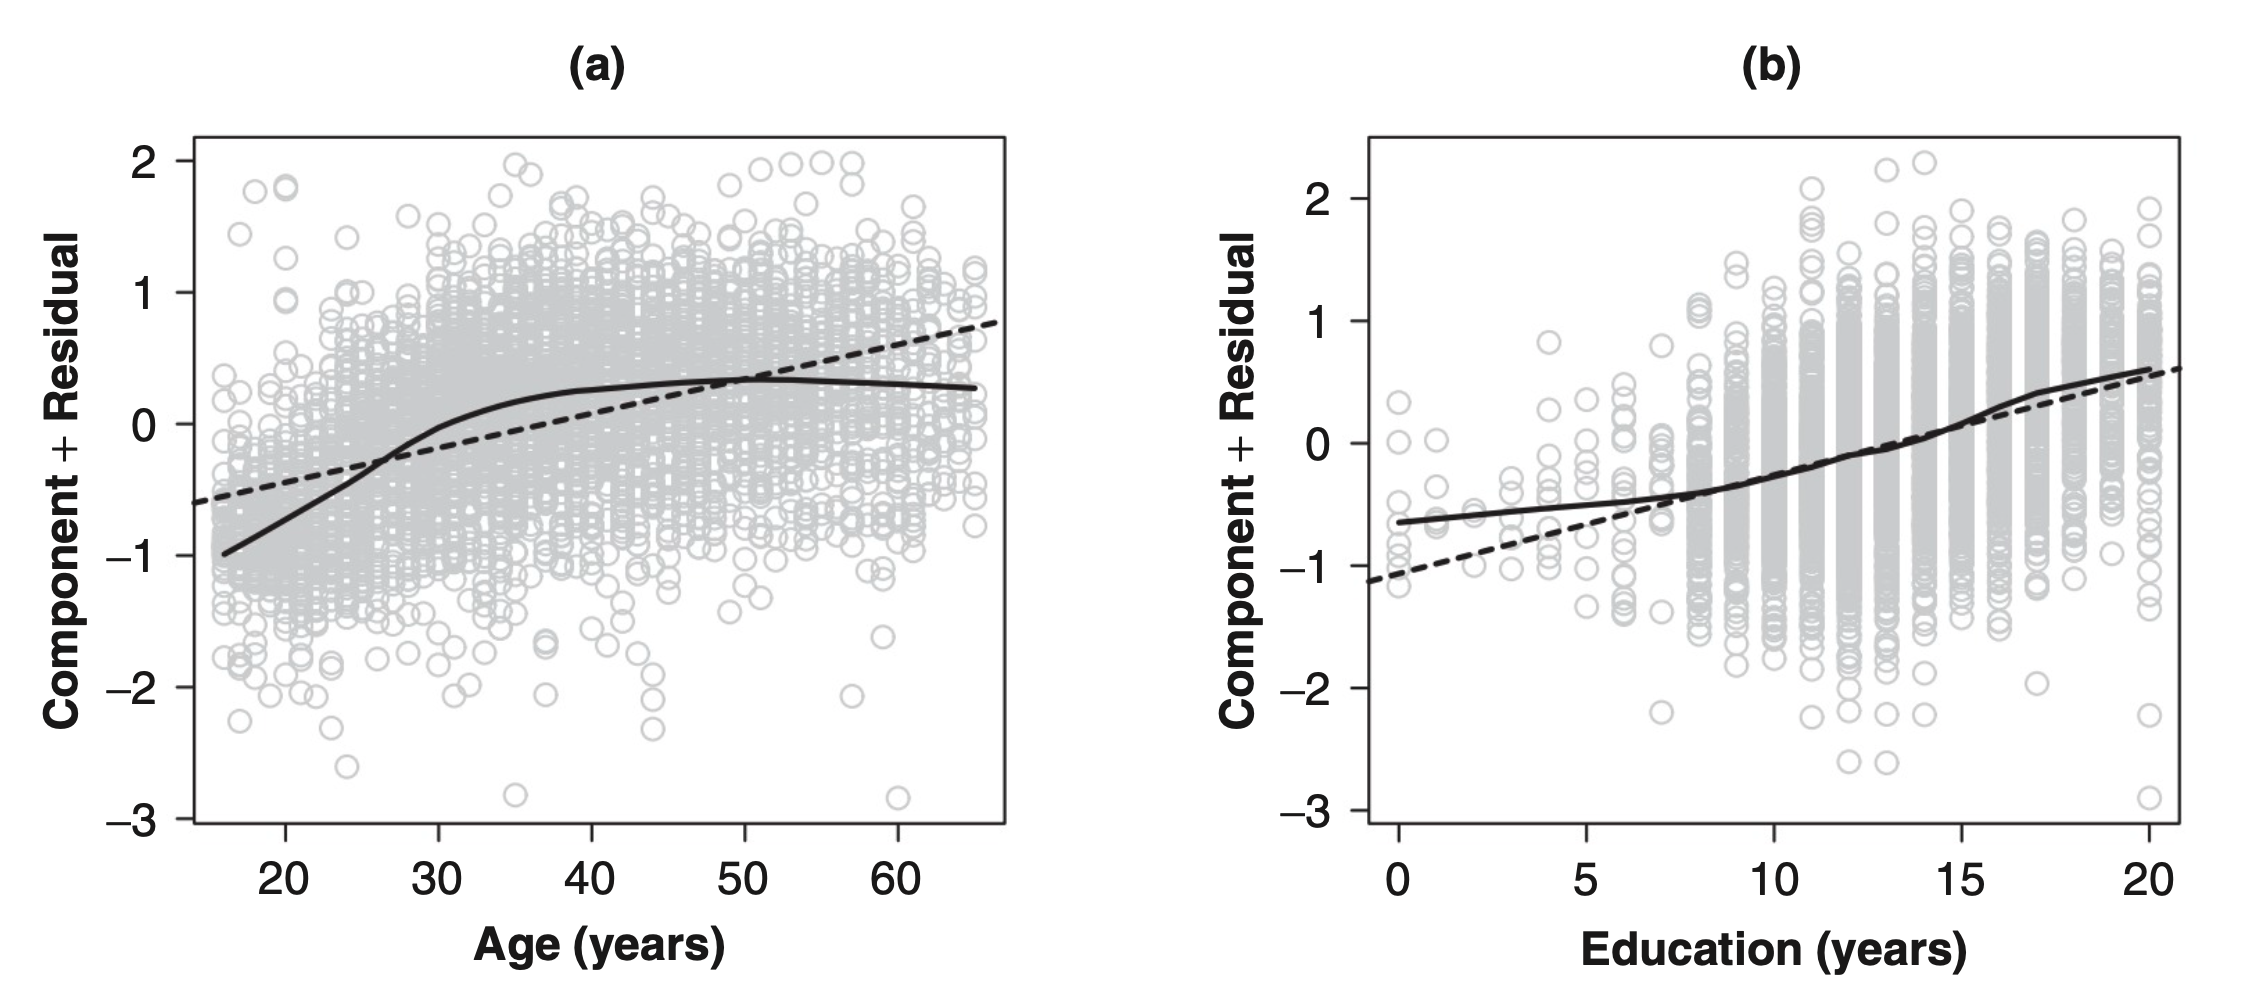
\includegraphics[width=0.9\textwidth]{Lecture19/JF_12_6}
  \caption{
  Component-plus-residual plots for age and education in SLID regression of log wages on these variables and sex.
  The solid lines are for lowess smooths with spans of $0.4$, and the broken lines are for linear least-squares fits.
   JF Figure 12.6.}
  \label{fig:JF_12_6}
\end{center}
\end{figure}
%



\subsection*{Data transformation}

%\subsubsection*{Transforming nonconstant spread, JF 4.4}
%An application of Tukey's rule for selecting a transformation is to use the linear ``trend'' of the spread-level plot to suggest a spread-stabilizing power transformation of the data.
%Express the linear fit as:
%$$
%\log \mbox{spread} \approx a + b \log \mbox{level}
%$$
%Then the corresponding spread-stabilizing transformation uses the power $p = 1 - b$ for the Box-Cox family of power transformation.

\subsubsection*{The family of powers and Roots, JF 4.1}
A particularly useful group of transformations is the ``family'' of powers and roots:
$$
X \to X^p
$$
wehre the arrow indicates that we intend to replace $X$ with the transformed variable $X^p$.
If $p$ is negative, then the transformation is an inverse power. For example, $X^{-1} = 1/X$.
If $p$ is a fraction, then the transformation represents a root.  For example, $X^{1/3} = \sqrt[3]{X}$.

It is more convenient to define the family of power transformations in a slightly more complex manner, called the \underline{Box-Cox family} of transformations (introduced in a seminal paper on transformations by Box \& Cox, 1964):
$$
X \to X^{(p)} = \frac{X^p - 1}{p}
$$

Because $X^{(p)}$ is a linear function of $X^p$, the two transformations have the same essential effect on the data, but, as is apparent in Figure~\ref{fig:JF_4_1}
%
\begin{figure}[H]
\begin{center}
  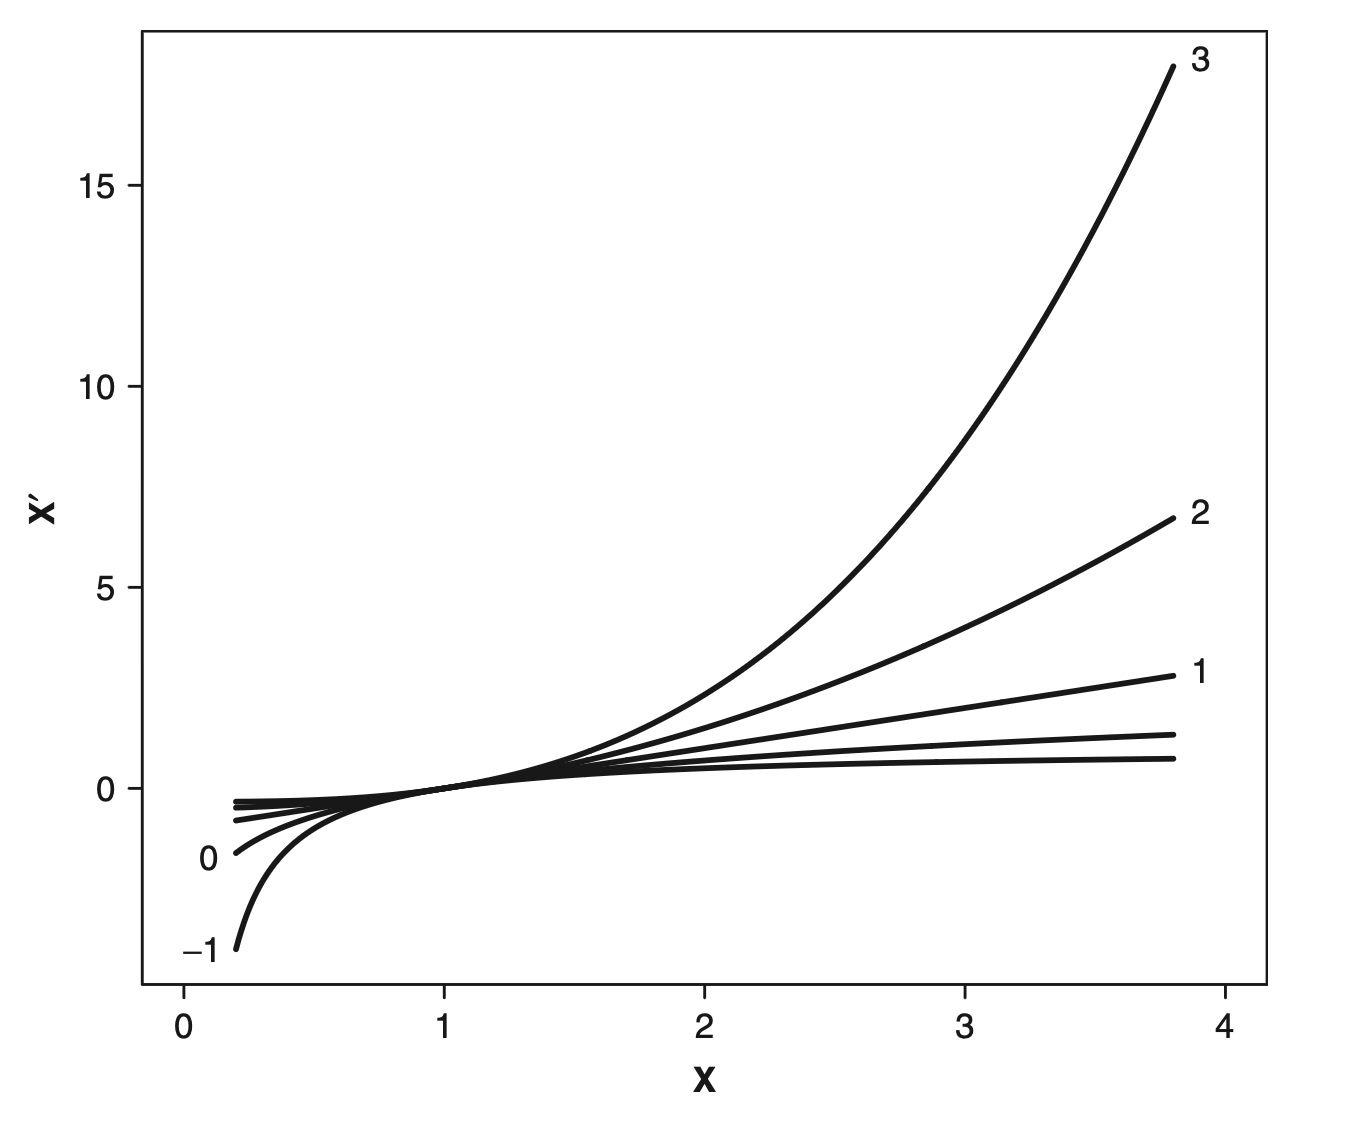
\includegraphics[width=0.8\textwidth]{Lecture18/JF_4_1}
  \caption{The Box-Cox family of power transformations $X'$ of $X$.
  The curve labeled $p$ is the transformation $X^{(p)}$, that is $(X^p - 1)/p$; $X^{(0)}$ is $\log_e(X)$.
   JF Figure 4.1.}
  \label{fig:JF_4_1}
\end{center}
\end{figure}
%
\begin{itemize}
  \item Dividing by $p$ preserves the direction of $X$, which otherwise would be reversed when $p$ is negative.
  \item The transformations $X^{(p)}$ are ``matched'' above $X=1$ both in level and in slope:
    \begin{enumerate}
      \item $1^{(p)} = 0$, for all values of $p$
      \item each transformation has a slope of $1$ at $X=1$.
    \end{enumerate}
  \item Descending the ``ladder'' of powers and roots towards $X^{(-1)}$ compresses the large values of $X$ and spreads out the small ones.
  Ascending the ladder of powers and roots towards $X^{(2)}$ has the opposite effect.
  As $p$ moves further from $p=1$ (i.e.~no transformation) in either direction, the transformation grows more powerful, increasingly ``bending'' the data.
  \item The power transformation $X^0$ is useless because it changes all values to $1$, but we can think of the log transformation as a kind of ``zeroth'' power:
  $$
  \lim\limits_{p \to 0} \frac{X^p - 1}{p} = \log_e X
  $$
  and by convention, $X^{(0)} \equiv \log_e X$.
\end{itemize}

\subsubsection*{Box-Cox transformation of $Y$}

Box and Cox (1964) suggested a power transformation of $Y$ with the object of normalizing the error distribution, stabilizing the error variance, and straightening the relationship of $Y$ to the $X$s.
The general Box-Cox model is
$$
Y_i^{(\lambda)} = \beta_0 + \beta_1 X_{i1} + \dots + \beta_p X_{ip} + \epsilon_i
$$
where $\epsilon_i \distas{iid} N(0, \sigma_\epsilon^2)$, and 
$$
Y_i^{(\lambda)} = \left\{ \begin{array}{ll}  
\frac{Y_i^\lambda - 1}{\lambda} & \mbox{for } \lambda \ne 0\\
\log_e Y_i & \mbox{for } \lambda = 0\\
 \end{array} \right.
$$
Note: in statistics, $\log_e$ is often written as $\log$.

For a particular choice of $\lambda$, the conditional maximized log-likelihood (see JF 12.5.1 p.324 footnote 55) is
$$
\begin{aligned}
\log_e L(\beta_0, \beta_1, \dots, \beta_p, \sigma_\epsilon^2 | \lambda) &= - \frac{n}{2} (1 + \log_e 2\pi)  \\
&-\frac{n}{2}\log_e \hat{\sigma}_\epsilon^2(\lambda) + (\lambda - 1)\sum\limits_{i = 1}^n \log_e Y_i\\
\end{aligned}
$$
where $\hat{\sigma}_\epsilon^2(\lambda) = \sum \hat{\epsilon}_i^2(\lambda) / n$ and where $\hat{\epsilon}_i(\lambda)$ are the residuals from the least-squares regression of $Y^{(\lambda)}$ on $X$s.
The least-squares coefficients from this regression are the maximum-likelihood estimates of $\beta$s conditional on the values of $\lambda$.

A simple procedure for finding the maximum-likelihood estimator $\hat{\lambda}$ is to evaluate the maximized $\log_e L$ (called the \underline{profile log-likelihood}) for a range of values of $\lambda$.
To test:$H_0: \lambda = 1$, calculated the likelihood-ratio statistic
$$
G_0^2 = -2 [\log_e L(\lambda = 1) - \log_e L(\lambda = \hat{\lambda})]
$$
which is asymptotically distributed as $\chi^2_1$ with one degree of freedom under $H_0$.
A 95\% confidence interval for $\lambda$ includes those values for which
$$
\log_e L(\lambda) > \log_e L(\lambda = \hat{\lambda}) - 1.92
$$
The number $1.92$ comes from $\frac{1}{2}\chi^2_{1, 0.05} = 0.5 \times 1.96^2$.

Figure~\ref{fig:JF_12_14} shows a plot of the profile log-likelihood against $\lambda$ for the original SLID regression of composite hourly wages on sex, age,  and education.
The maximum-likelihood estimate of $\lambda$ is $\hat{\lambda} = 0.09$, and a 95\% confidence interval runs from $0.04$ to $0.13$.
Although $0$ is outside of the CI (confidence interval), it is essentially the same transformation of wages as $\lambda=0.09$ (the correlation between log wages and wages${}^{0.09}$ is $0.9996$).
%
\begin{figure}[H]
\begin{center}
  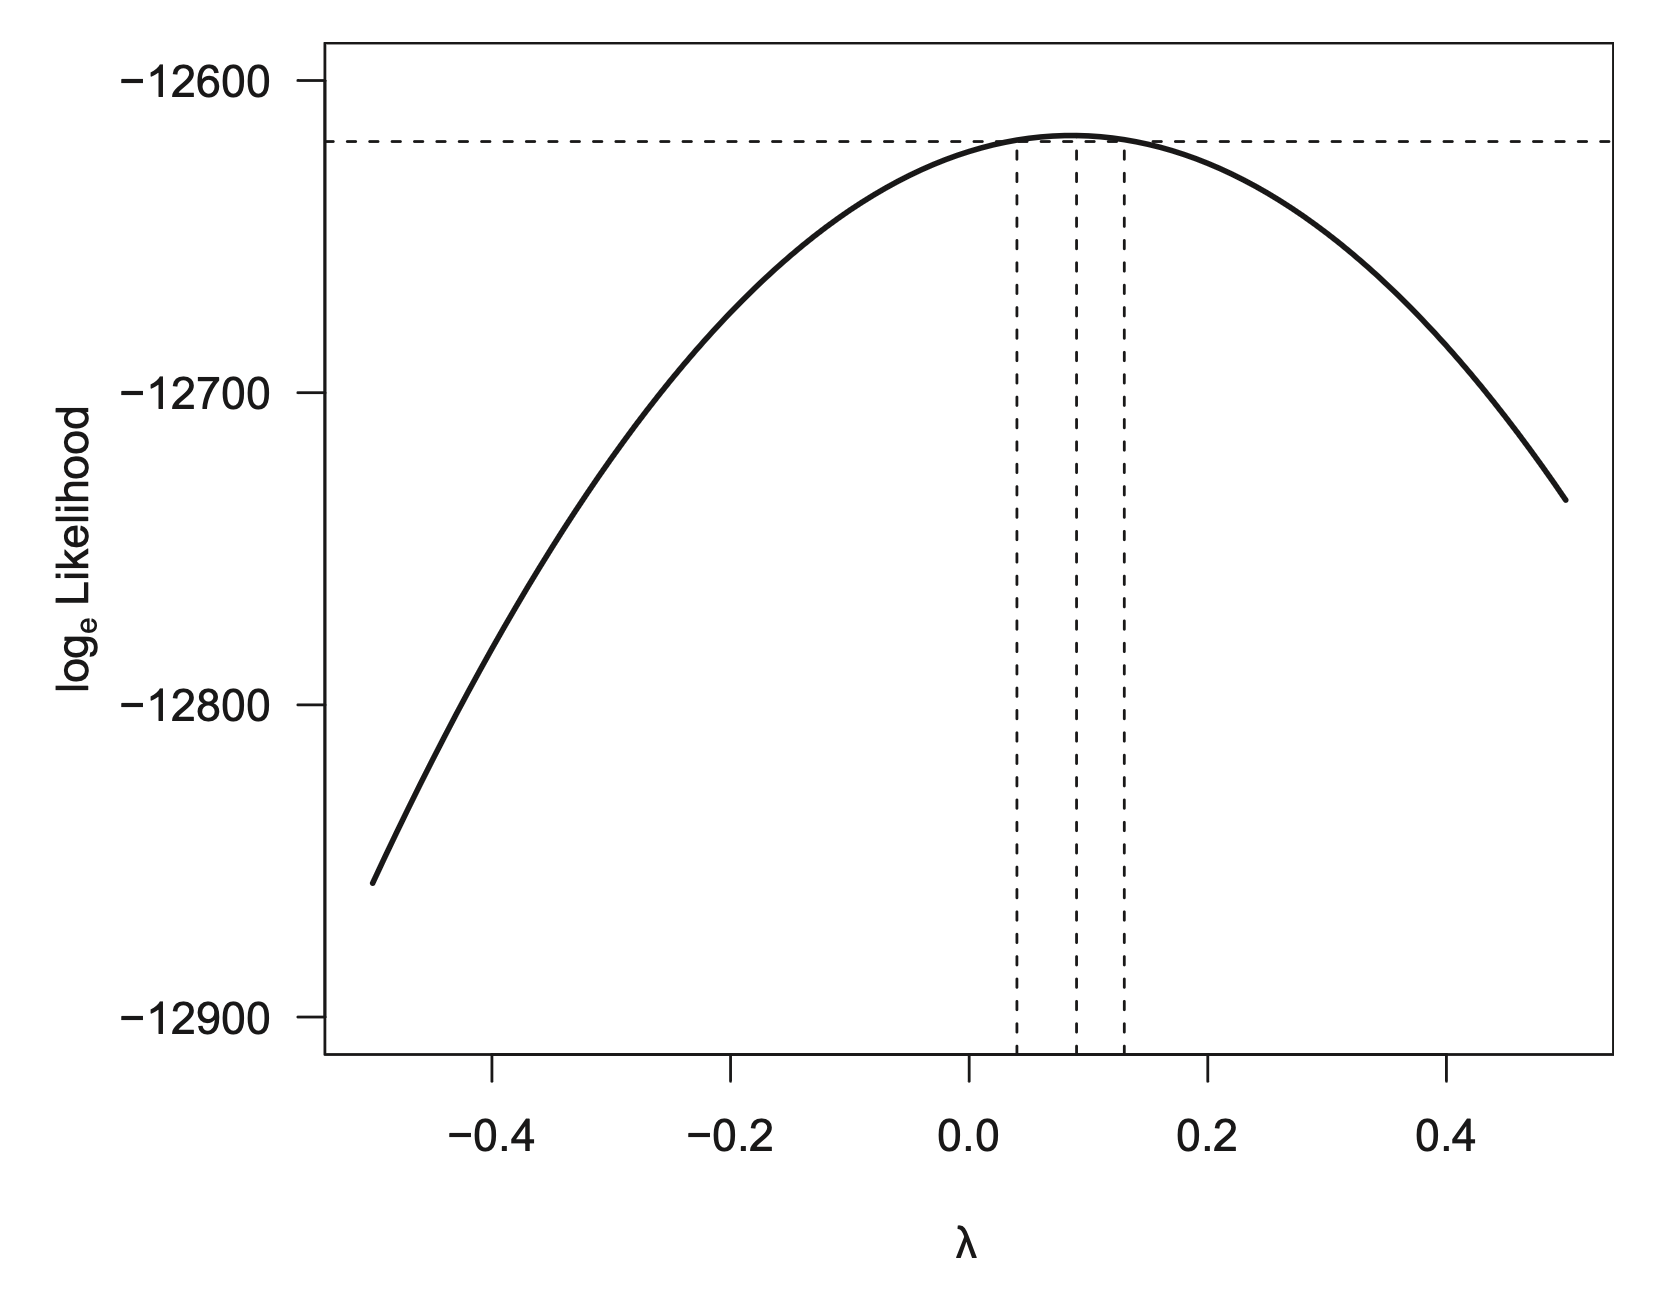
\includegraphics[width=0.6\textwidth]{Lecture19/JF_12_14}
  \caption{
  Box-Cox transformations for the SLID regression of wages on sex, age, and education.
  The maximized (profile) log-likelihood is plotted against the transformation parameter $\lambda$.
  The intersection of the line near the top of the graph with the profile log-likelihood curve marks off a 95\% confidence interval for $\lambda$.
  The maximum of the log-likelihood corresponds to the MLE of $\lambda$.
   JF Figure 12.14.}
  \label{fig:JF_12_14}
\end{center}
\end{figure}
%

\subsubsection*{Box-Tidwell transformation of $X$s}

Now, consider the model
$$
Y_i = \beta_0 + \beta_1 X_{i1}^{\gamma_1} + \dots +  \beta_p X_{ip}^{\gamma_p}  + \epsilon_i
$$
where the errors are independently distributed as $\epsilon_i \distas{iid} N(0, \sigma_\epsilon^2)$ and all the $X_{ij}$ are positive.

The parameters of this model ($\beta_0, \beta_1, \dots, \beta_p, \gamma_1, \dots, \gamma_p$, and $\sigma_\epsilon^2$) could be estimated by general nonlinear least squares.
Box and Tidwell (1962) suggested the following computationally more efficient procedure (also yields a constructed-variable diagnostic):
\begin{enumerate}
  \item Regress $Y$ on $X_1, \dots, X_p$, obtaining $\hat{\beta}_0, \hat{\beta}_1, \dots, \hat{\beta}_p$.  (``Regress $A$ on $B$s'' is the same as ``fitting the linear regression model with $A$ as the response variable and $B$s as the explanatory variables''.)
  \item Regress $Y$ on $X_1, \dots, X_p$ and the \underline{constructed variables} $X_1 \log_e X_1, \dots, X_p \log_e X_p$ (again, by fitting the model of $Y = \beta_0 + \beta_1 X_1 + \dots + \beta_p X_p + \delta_1 X_1 \log_e X_1 + \dots + \delta_p X_p \log_e X_p + \epsilon_i$) to obtain $\tilde{\beta}_0, \tilde{\beta}_1, \dots, \tilde{\beta}_p, \tilde{\delta}_1, \dots, \tilde{\delta}_p$.
  In general $\hat{\beta}_i \ne \tilde{\beta}_i$.  (The constructed variables result from the first-order Taylor-series approximation to $X_j^{\gamma_j}$ evaluated at $\gamma_j = 1$: $ X_j^{\gamma_j} \approx X_1 + (\gamma_1 - 1) X_1 \log_e X_1 $. )
  \item The constructed variable $X_j \log_e X_j$ can be used to assess the need for a transformation of $X_j$ by testing the null hypothesis $H_0:\delta_j = 0$.
  Added-variable plots for the constructed variables are useful for assessing leverage and influence on the decision to transform the $X$s.
  \item A preliminary estimate of the transformation parameter $\gamma_j$ (not the MLE) is
  $$
  \tilde{\gamma_j} = 1 + \frac{\tilde{\delta}_j}{\hat{\beta}_j}
  $$
  where $\tilde{\delta}_j$ is from step 2 and $\hat{\beta}_j$ is from step 1.
\end{enumerate}

\subsection*{Polynomial regression}
A machinery of multiple regression to fit non-linear relationships between predictor(s) and response.
\begin{itemize}
  \item Linear: $y = \beta_0 + \beta_1 x + \epsilon$
  \item Quadratic: $y = \beta_0 + \beta_1 x + \beta_2 x^2 + \epsilon$
  \item Cubic: $y = \beta_0 + \beta_1 x  +\beta_2 x^2 + \beta_3 x^3 + \epsilon$ 
  \item $k^{th}$ order polynomial:  $y = \beta_0 + \beta_1 x + \beta_2 x^2 + \dots +\beta_k x^k + \epsilon$
\end{itemize}

Question:\\
Does quadratic model provide a significantly better fit than linear model?\\
{\it Solution: }Test $H_0: \beta_2 = 0$ vs. $H_a: \beta_2 \ne 0$.\\
Alternatively, compare the corresponding adjusted-$R^2$ values.
















\newpage
\setcounter{section}{20}

\section{Lecture 21: March 15}


\subsection*{Last time}
\begin{itemize}
	\item Diagnosing nonlinearity (JF chapter 12)
	\item Data transformation (JF chapter 4)
\end{itemize}


\subsection*{Today}
\begin{itemize}
	\item Collinearity (JF chapter 13, RD 8.3.2)
	\item Principal component analysis (JF 13.1.1, RD 8.3.4)
%	\item Biased estimation:
%	  \begin{itemize}
%	  	\item Ridge Regression
%	  	\item Lasso Regression
%	  \end{itemize}
\end{itemize}

\subsubsection*{Additional reference}
``A First Course in Linear Model Theory'' by Nalini Ravishanker and Kipak K. Dey.

\subsection*{Collinearity}

In linear model
$$
\begin{aligned}
	\mathbf{Y} &= \vecc{X} \mathbf{\beta} + \mathbf{\epsilon}\\
	\epsilon &\sim \mathcal{N}(0, \sigma^2 \mathbf{I}_n)\\
\end{aligned}
$$

\underline{Collinearity (or multicollinearity)} exists when there is ``near-dependency'' between the columns of the design matrix $\vecc{X}$.
	\begin{itemize}
	\item Two or more columns.
	\item In other words, high correlation between explanatory variables.
	\item the data/model pair is  ill-conditioned when $\vecc{X} \transpose \vecc{X}$ is nearly singular.
\end{itemize}

Perfect collinearity leads to rank-deficiency in $\vecc{X}$ such that $\vecc{X} \transpose \vecc{X}$ is singular.
In the case of perfect collinearity, two or more columns are linear-dependent.

\subsubsection*{An example of perfect collinearity}
\begin{equation*}
	Y_i = \beta_0 + \beta_1 X_{i1} + \beta_2 X_{i2} + \beta_3 X_{i3} + \beta_4 X_{i4}  + \beta_5 X_{i5} + \epsilon_i
\end{equation*}

Consider the case, where
\begin{itemize}
	\item $Y_i$ represents the amount of sales.
	\item $X_{i1}, X_{i2}, ..., X_{i4}$ are categorical that represent the quarter in which the sample is collected: $X_{ij} = \mathbf{1}(\mbox{sample } i \mbox{ collected in quarter } j)$.
	\item $X_{i5}$ represents expense spent in advertising.
\end{itemize}

The \underline{dummy variable trap} $X_{i4} = 1 - X_{i1} - X_{i2} - X_{i3}$.  Recall that we need $m-1$ dummy variables for $m$ categories.

\subsubsection*{An example of high correlation between predictors}

\begin{equation*}
	Y_i = \beta_0 + \beta_1 X_{i1} + \beta_2 X_{i2} + \epsilon_i
\end{equation*}

Consider the case, where
\begin{itemize}
	\item $Y_i$ represents the salary of individual $i$.
	\item $X_{i1}$ represents the age of individual $i$.
	\item $X_{i2}$ represents the experience of individual $i$.
\end{itemize}

{How to interpret $\beta_1$?}

We expect high correlation between age and experience.


\subsubsection*{Problems caused by multicollinearity}

\begin{enumerate}
	\item large standard errors of the regression coefficients
	\begin{itemize}
		\item small associated t-statistics
		\item conclusion that truly useful explanatory variables are insignificant in explaining the regression
	\end{itemize}
	\item the sign of regression coefficients may be the opposite of what a mechanistic understanding of the problem would suggest
	\item deleting a column of the predictor matrix will cause large changes in the coefficient estimates for other variables
\end{enumerate}

However, multicollinearity does {\bf not} greatly affect the {\bf predicted values}.

\subsubsection*{Signs and detections of multicollinearity}
\newcommand{\xstatistics}[1]{{\it #1}-statistics}
Some signs for multicollinearity:
\begin{enumerate}
	\item Simple correlation between a pair of predictors exceeds $0.9$ or $R^2$.
	\item High value of the multiple correlation coefficient with some high partial correlations between the explanatory variables.
	\item Large \xstatistics{F} with some small \xstatistics{t} for individual regression coefficients
\end{enumerate}


Some approaches for detecting multicollinearity:
\begin{enumerate}
	\item Pairwise correlations among the explanatory variables
	\item Variance inflation factor
	\item Condition number
\end{enumerate}


\subsubsection*{Variance inflation factor}

For a multiple linear regression with $k$ explanatory variables.
We can regress $X_j$ on the $(k-1)$ other explanatory variables and denote $R_j$ as the coefficient of determination.

Then the \underline{variance inflation factor} (VIF) is defined as
\begin{equation*}
	\mbox{VIF}_j = \frac{1}{1 - R_j^2}
\end{equation*}

\begin{itemize}
	\item $\mbox{VIF}_j \in [1, +\infty)$
	\item A suggested threshold is $10$
	\item May use the averaged $\overline{\mbox{VIF}}=\sum\limits_{j=1}^k{\mbox{VIF}_j}\bigg/ k$.
\end{itemize}

\subsubsection*{Condition index and condition number}
We first scale the design matrix $\vecc{X}$ into column-equilibrated predictor matrix $\vecc{X}_E$
such that $\{X_E\}_{ij} = X_{ij} / \sqrt{\vecc{X}_j\transpose \vecc{X}_j}$.

Let $\vecc{X}_E=\mathbf{U}\mathbf{D}\mathbf{V}\transpose$ be the singular-value decomposition (SVD) of
the $n \times p$ matrix $\vecc{X}_E$
where $\mathbf{U}\transpose \mathbf{U} = \mathbf{V}\transpose \mathbf{V} = \mathbf{I}_p$
and $\mathbf{D} = diag(d_1, d_2, ..., d_p)$ is a diagonal matrix with $d_j \ge 0$.

\vspace{1.5em}
The $j^{th}$ \underline{condition index} is defined as 
\begin{equation*}
	\eta(\vecc{X}_E) = d_{\max} / d_j, \mbox{      } j=1, 2, ..., p
\end{equation*}

\vspace{0.5em}
The \underline{condition number} is defined as
\begin{equation*}
	C = d_{\max} / d_{\min}
\end{equation*}
$C \ge 1$, $d_{\max}=\max\limits_{1 \le j \le p}d_j$ and $d_{\min}=\min\limits_{1 \le j \le p}d_j$

Some properties of the condition number
\begin{itemize}
	\item Large condition number indicates evidence of multicollinearity
	\item Typical cutoff values, 10, 15 to 30.
\end{itemize}

Some problems with the condition number
\begin{itemize}
	\item practitioners have different opinions of whether $\vecc{X}$ should be centered around their means for SVD. 
	\begin{itemize}
		\item centering may remove nonessential ill conditioning, e.g. $Cor(X, X^2)$
		\item centering may mask the role of the constant term in any underlying near-dependencies
	\end{itemize}
	\item the degree of multicollinearity with dummy variables may be influenced by the choice of reference category
	\item condition number is affected by the scale of the $\vecc{X}$ measurements
	\begin{itemize}
		\item By scaling down any column of $\vecc{X}$, the condition number can be made arbitrarily large
		\item Known as {\it artificial ill-conditioning}
		\item The condition number of the scaled matrix $\vecc{X}_E$ is also referred to as the {\it scaled condition number}
	\end{itemize}
\end{itemize}

Recall that $\vecc{X}_E=\mathbf{U}\mathbf{D}\mathbf{V}\transpose$ is the singular-value decomposition (SVD) of $\vecc{X}_E$,
where $\mathbf{U}\transpose \mathbf{U} = \mathbf{V}\transpose \mathbf{V} = \mathbf{I}_p$
and $\mathbf{D} = diag(d_1, d_2, ..., d_p)$ is a diagonal matrix with $d_j \ge 0$.

\vspace{2em}
Then
\vspace{1em}
\begin{equation*}
	\begin{aligned}
		\vecc{X}_E\transpose \vecc{X}_E &= \mathbf{V}\mathbf{D}\mathbf{U}\transpose\mathbf{U}\mathbf{D}\mathbf{V}
		\transpose \\
		&= \mathbf{V}\mathbf{D}^2 \mathbf{V}\transpose\\
	\end{aligned}
\end{equation*}
\vspace{1em}

is the spectral decomposition of the Gramian matrix $\vecc{X}_E\transpose \vecc{X}_E$ with $\{d_j^2\}$ being the eigenvalues and $\mathbf{V}$ being the corresponding eigen vector matrix.
This relationship links the condition numbers to the eigen values of the Gramian matrix.

\subsubsection*{Variance decomposition method}

The variance-covariance matrix of the coefficient
\begin{equation*}
	\begin{aligned}
		Cov(\hat{\beta}) 
		&= \sigma^2 (\vecc{X}_E\transpose \vecc{X}_E)^{-1} \\
		&= \sigma^2 \mathbf{V}\mathbf{D}^{-2} \mathbf{V}\transpose\\
	\end{aligned}
\end{equation*}

Its $j^{th}$ diagonal element is the estimated variance of the $j^{th}$ coefficient, $\hat{\beta}_j$.
Then
\begin{equation*}
	Var(\hat{\beta}_j) 
	= \sigma^2 \sum\limits_{h=1}^p{\frac{v_{jh}^2}{d_h^2}}
\end{equation*}


\begin{itemize}
	\item Let $q_{jh} = \frac{v_{jh}^2}{d_h^2}$ and $q_j = \sum\limits_{h=1}^p {q_{jh}}$.
	\item The variance decomposition proportion is $\pi_{jh} = q_{jh}/q_j$.
	\item $\pi_{jh}$ denotes the proportion of the variance of the $j^{th}$ regression coefficient associated with the $h^{th}$ component of its decomposition.
	\item The variance decomposition proportion matrix is $\mathbf{\Pi} = \{\pi_{jh}\}$.
\end{itemize}

In practice, it is suggested to combine condition index and proportions of variance for multicollinearity diagnostic.
\begin{table*}
	\centering
	\begin{tabular}{lcccc}
		\toprule
		Condition & \multicolumn{4}{c}{Proportions of variance}\\
		Index & $Var(\hat{\beta}_1)$ & $Var(\hat{\beta}_2)$ & ... & $Var(\hat{\beta}_3)$\\ 
		\hline
		$\eta_1$ & $\pi_{11}$ & $\pi_{12}$ & ... & $\pi_{1p}$\\
		$\eta_2$ & $\pi_{21}$ & $\pi_{22}$ & ... & $\pi_{2p}$\\
		\vdots & \vdots & \vdots & & \vdots\\
		$\eta_p$ & $\pi_{p1}$ & $\pi_{p2}$ & ... & $\pi_{pp}$\\
		\bottomrule
	\end{tabular}
	\caption{
		Table of condition index and proportions of variance}
\end{table*}
Identify multicollinearity if
\begin{itemize}
	\item Two or more elements in the $j^{th}$ row of matrix $\mathbf{\Pi}$ are relatively large
	\item And its associated condition index $\eta_j$ is large too
\end{itemize}

\subsection*{Principal Components}

The method of principal components, introduced by Karl Pearson (1901) and Harold Hotelling (1933), provides a useful representation of the correlational structure of a set of variables.
Some advantages of the principal component analysis include
\begin{itemize}
	\item more unified
	\item linear transformation of the original predictors into a new set of orthogonal predictors
	\item the new orthogonal predictors are called principal components
\end{itemize}

Principal components regression is an approach that inspects the sample data $(\vecc{Y}, \vecc{X})$ for directions of variability and uses this information to reduce the dimensionality of the estimation problem.
The procedure is based on the observation that every linear regression model can be restated in terms of a set of orthogonal predictor variables, which are constructed as linear combinations of the original variables.
The new orthogonal variables are called the \underline{principal components} of the original variables.

Let $\vecc{X} \transpose \vecc{X} = \vecc{Q} \vecc{\Delta} \vecc{Q}\transpose $ denote the spectral decomposition of $\vecc{X} \transpose \vecc{X}$, where $\vecc{\Delta} = diag\{\lambda_1, \dots, \lambda_p\}$ is a diagonal matrix consisting of the (real) eigenvalues of $\vecc{X} \transpose \vecc{X}$,
with $\lambda_1 \ge \dots \ge \lambda_p$ and $\vecc{Q} = (\vecc{q_1}, \dots, \vecc{q_p})$ denotes the matrix whose columns are the orthogonal eigenvectors of $\vecc{X} \transpose \vecc{X}$ corresponding to the ordered eigenvalues.
Consider the transformation
$$
\vecc{Y} = \vecc{X}\vecc{Q}\vecc{Q}\transpose \vecc{\beta} + \vecc{\epsilon} = \vecc{Z}\vecc{\theta} + \vecc{\epsilon},
$$
where $\vecc{Z} = \vecc{XQ}$, and $\vecc{\theta} = \vecc{Q}\transpose \vecc{\beta}$.\\
The elements of $\vecc{\theta}$ are known as the \underline{regression parameters of the principal components}.
The matrix $\vecc{Z} = \{\vecc{z_1}, \dots, \vecc{z_p}\}$ is called the matrix of principal components of $\vecc{X} \transpose \vecc{X}$.
$\vecc{z}_j = \vecc{X}\vecc{q}_j$ is the $j$th principal component of $\vecc{X} \transpose \vecc{X}$ and $\vecc{z}_j\transpose \vecc{z}_j = \lambda_j$, the $j$th largest eigenvalue of $\vecc{X} \transpose \vecc{X}$.

Principal components regression consists of deleting one or more of the variables $\vecc{z}_j$ (which correspond to small values of $\lambda_j$), and using OLS estimation on the resulting reduced regression model.

\subsubsection*{Derivation under standardized predictors, JF 13.1.1}
Consider the vectors of standardized predictors, $\vecc{x}^*_1,\vecc{x}^*_2, \dots, \vecc{x}^*_p$ (obtained by subtracting the mean and divided by standard deviation of the original predictor vectors).
Because the principal components are linear combinations of the original predictors, we write the first principal component as
$$
\begin{aligned}
\vecc{w}_1 &= A_{11} \vecc{x}^*_1 + A_{21} \vecc{x}^*_2 + \cdots + A_{p1} \vecc{x}^*_p\\
&= \vecc{X}^* \vecc{a}_1\\
\end{aligned}
$$
The variance of the first component becomes
$$
\begin{aligned}
S_{w_1}^2 &= \frac{1}{n - 1} \vecc{w}_1\transpose \vecc{w}_1 \\
&= \frac{1}{n - 1} \vecc{a}_1 \transpose {\vecc{X}^*}\transpose \vecc{X}^* \vecc{a}_1\\
&= \vecc{a}_1\transpose \vecc{R}_{XX}\vecc{a}_1\\
\end{aligned}
$$
where $\vecc{R}_{XX} = \frac{1}{n - 1}  {\vecc{X}^*}\transpose \vecc{X}^*$.
We want to maximize $S_{w_1}^2$ under the normalizing constraint $\vecc{a}_1\transpose \vecc{a}_1 = 1$ (otherwise $S_{w_1}^2$ can be arbitrarily large by inflating $\vecc{a}_1$).
Consider
$$
F_1 \equiv \vecc{a}\transpose \vecc{R}_{XX} \vecc{a}_1 - L_1(\vecc{a}_1\transpose \vecc{a}_1 - 1)
$$
where $L_1$ is a Lagrange multiplier.  By differentiating this equation with respect to $\vecc{a}_1$ and $L_1$,
$$
\begin{aligned}
	\frac{\partial F_1}{\partial \vecc{a}_1} &= 2 \vecc{R}_{XX}\vecc{a}_1 - 2L_1 \vecc{a}_1\\
	\frac{\partial F_1}{\partial L_1} &= -(\vecc{a}_1 \transpose \vecc{a}_1 - 1)\\	
\end{aligned}
$$
Setting the partial derivatives to 0 produces
$$
\begin{aligned}
	(\vecc{R}_{XX} - L_1 \vecc{I}_p) \vecc{a}_1 &= \vecc{0}\\
	\vecc{a}_1 \transpose \vecc{a}_1 &= 1\\	
\end{aligned}
$$
From the first equation, we see that $L_1$ is an eigenvalue of $\vecc{R}_{XX}$ such that $\vecc{R}_{XX} \vecc{a}_1 = L_1 \vecc{a}_1$ such that
$$
S_{w_1}^2 = \vecc{a}_1\transpose \vecc{R}_{XX}\vecc{a}_1 = L_1\vecc{a}_1\transpose \vecc{a}_1 = L_1
$$
To maximize $S_{w_1}^2$, we only need to pick the largest eigenvalue of $\vecc{R}_{XX}$.














\newpage
\setcounter{section}{21}

\section{Lecture 22: March 17}


\subsection*{Last time}
\begin{itemize}
	\item Collinearity (JF chapter 13, RD 8.3.2)
\item Principal component analysis (JF 13.1.1, RD 8.3.4)
\end{itemize}


\subsection*{Today}
\begin{itemize}
	\item Midterm exam review
	\item Biased estimation (JF 13.2.3, CG's notes)
	\begin{itemize}
		\item Ridge regression
		\item Lasso regression
	\end{itemize}
\end{itemize}

\subsubsection*{Additional reference}
\href{https://math.bu.edu/people/cgineste/classes/ma575/p/w14_1.pdf}{Lecture notes} by Cedric Ginestet

\subsection*{Ridge Regression}

Ridge regression and the Lasso regression are two forms of \underline{regularized regression}.
These methods can be used to alleviate the consequences of multicollinearity.

\begin{enumerate}
	\item When variables are highly correlated, a large coefficient in one variable may be alleviated by a large coefficient in another variable, which is negatively correlated to the former.
	\item Regularization imposes an upper threshold on the values taken by the coefficients, thereby producing a more parsimonious solution, and a set of coefficients with smaller variance.
\end{enumerate}

\subsubsection*{Constrained optimization}

Ridge regression is motivated by a constrained minimization problem, which can be formulated as
$$
\begin{aligned}
&\hat{\beta}^{ridge} = \argmin\limits_{\beta \in \mathbb{R}^p} \sum\limits_{i = 1}^n(y_i - \vecc{x}_i\transpose \beta)^2\\
&\mbox{subject to } ||\beta||_2^2 = \sum\limits_{j = 1}^p \beta_j^2 \le t \\
\end{aligned}
$$
for $t \ge 0$.  

Use a Lagrange multiplier, we can rewrite the formula as
$$
\hat{\beta}^{ridge} =\argmin\limits_{\beta \in \mathbb{R}^p} \{  \sum\limits_{i = 1}^n(y_i - \vecc{x}_i\transpose \beta)^2 + \lambda \sum\limits_{j = 1}^p \beta_j^2\}
$$
for $\lambda \ge 0$ and where there is a one-to-one correspondence between $t$ and $\lambda$.
$\lambda$ is an arbitrary constant usually referred to as the ``ridge constant''.

\subsubsection*{Analytical solutions}
The ridge-regression estimator has analytical solution
$$
\hat{\beta}^{ridge} = (\vecc{X}\transpose\vecc{X} + \lambda \vecc{I})^{-1} \vecc{X}\transpose \vecc{Y}
$$
This is obtained by differentiating the objective function with respect to $\beta$ and set it to $0$:
$$
\begin{aligned}
&\frac{\partial}{\partial \beta} \{(\vecc{Y} - \vecc{X}\beta)\transpose (\vecc{Y} - \vecc{X}\beta) +\lambda \vecc{\beta}\transpose \vecc{\beta}\}\\
=& 2(\vecc{X}\transpose \vecc{X}) \beta - 2 \vecc{X}\transpose \vecc{Y} + 2\lambda \beta \\
=& 0\\
\end{aligned}
$$
Therefore,
$$
(\vecc{X}\transpose\vecc{X} + \lambda \vecc{I})\vecc{\beta} = \vecc{X}\transpose\vecc{Y}
$$

Since we are adding a positive constant to the diagonal of $\vecc{X}\transpose\vecc{X}$, we  are , in general, producing an invertible matrix, $\vecc{X}\transpose\vecc{X} + \lambda\vecc{I}$ even if $\vecc{X}\transpose\vecc{X}$ is singular.  Historically, this particular aspect of ridge regression was the main motivation behind the adoption of this particular extension of OLS theory.

The ridge regression estimator is related to the classical OLS estimator, $\hat{\beta}^{OLS}$, in the following manner
$$
\hat{\beta}^{ridge}  = \left[\vecc{I} + \lambda (\vecc{X}\transpose\vecc{X})^{-1}\right] ^{-1} \hat{\beta}^{OLS},
$$
assuming $\vecc{X}\transpose\vecc{X}$ is non-singular.  This relationship can be verified by applying the definition of $\hat{\beta}^{OLS}$,
$$
\begin{aligned}
\hat{\beta}^{ridge}  &= \left[\vecc{I} + \lambda (\vecc{X}\transpose\vecc{X})^{-1}\right] ^{-1} (\vecc{X}\transpose\vecc{X})^{-1} \vecc{X}\transpose\vecc{Y}\\
&=(\vecc{X}\transpose\vecc{X} + \lambda \vecc{I})^{-1} \vecc{X}\transpose \vecc{Y}\\
\end{aligned}
$$
using the fact $\vecc{B}^{-1}\vecc{A}^{-1} = \vecc{(AB)}^{-1}$.

Moreover, when $\vecc{X}$ is composed of orthonormal variables, such that $\vecc{X}\transpose\vecc{X} = \vecc{I}_p$, it then follows that 
$$
\hat{\beta}^{ridge} = \frac{1}{1 + \lambda} \hat{\beta}^{OLS}
$$

\subsubsection*{Bias and variance of ridge estimator}
Ridge estimation produces a biased estimator of the true parameter $\beta$.
With the definition of $\hat{\beta}^{ridge}$ and the model assumption $\Expected{\vecc{Y}|\vecc{X}} = \vecc{X}\vecc{\beta}$, we obtain,
$$
\begin{aligned}
\Expected{\hat{\beta}^{ridge} | \vecc{X}} &= (\vecc{X}\transpose\vecc{X} + \lambda \vecc{I})^{-1} \vecc{X}\transpose \vecc{X\beta}\\
&= (\vecc{X}\transpose\vecc{X} + \lambda \vecc{I})^{-1}  (\vecc{X}\transpose \vecc{X} + \lambda \vecc{I} - \lambda \vecc{I}) \vecc{\beta}\\
&= \beta - \lambda(\vecc{X}\transpose\vecc{X} + \lambda \vecc{I})^{-1} \vecc{\beta}\\
\end{aligned}
$$
where the bias of the ridge estimator is proportional to $\lambda$. 
The variance of the ridge estimator is
$$
\Var{\hat{\beta}^{ridge} | \vecc{X}} = \sigma^2 (\vecc{X}\transpose\vecc{X} + \lambda \vecc{I})^{-1} (\vecc{X}\transpose\vecc{X})  (\vecc{X}\transpose\vecc{X} + \lambda \vecc{I})^{-1}.
$$
When $\lambda$ increases, the inverted term $(\vecc{X}\transpose\vecc{X} + \lambda \vecc{I})^{-1}$ is increasingly dominated by $\lambda \vecc{I}$.
The variance of the ridge estimator, therefore, is a decreasing function of $\lambda$.
This result is intuitively reasonable because the estimator itself is driven toward $\vecc{0}$.

\subsubsection*{Variance-bias tradeoff}
The mean-squared error of an estimator can be decomposed into the sum of its squared bias and sampling variance.
$$
\begin{aligned}
MSE(\hat{\theta}) &= \Expected{(\hat{\theta} - \theta)^2} = \textbf{E}(\hat{\theta}^2) + \theta^2 - 2 \theta\textbf{E}(\hat{\theta}) \\
Bias^2(\hat{\theta}) &= \left[ \textbf{E}(\hat{\theta}) - \theta\right]^2 = \textbf{E}^2(\hat{\theta}) + \theta^2 - 2 \theta\textbf{E}(\hat{\theta}) \\
\text{Var}(\hat{\theta}) &= \textbf{E}(\hat{\theta}^2) - \textbf{E}^2(\hat{\theta})\\
\end{aligned}
$$
Therefore
$$
MSE(\hat{\theta}) = Bias^2(\hat{\theta}) + \text{Var}(\hat{\theta})
$$
The essential idea here is to trade a small amount of bias in the coefficient estimates for a large reduction in coefficient sampling variance.
Hoerl and Kennard (1970) prove that it is always possible to choose a positive value of the ridge constant $\lambda$ so that the mean-squared error of the ridge estimator is less than the mean-squared error of the least-squares estimator.
These ideas are illustrated heuristically in Figure~\ref{fig:13_9}
%
\begin{figure}[H]
	\begin{center}
		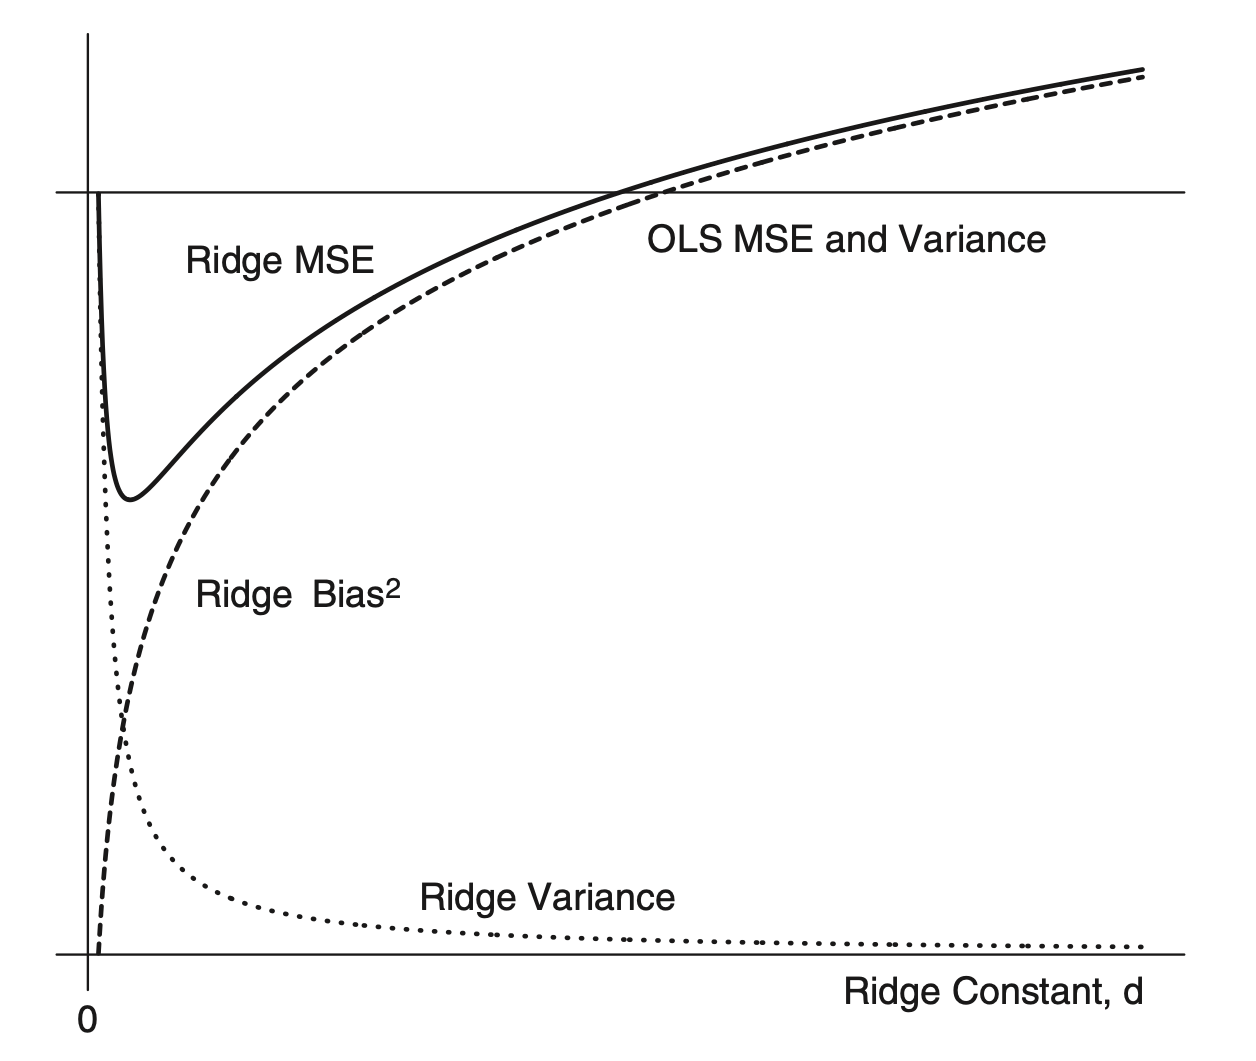
\includegraphics[width=0.7\textwidth]{Lecture22/JF_13_9}
		\caption{
			Trade-off of bias and against variance for the ridge-regression estimator.  
			The horizontal line gives the variance of the least-squares (OLS) estimator; because the OLS estimator is unbiased, its variance and mean-squared error are the same.
			The broken line shows the squared bias of the ridge estimator as an increasing function of the ridge constant $d$ (i.e.~$\lambda$ in our notes).
			The dotted line shows the variance of the ridge estimator.
			The mean-squared error (MSE) of the ridge estimator, given by the heavier solid line, is the sum of its variance and squared bias.
			For some values of $d$, the MSE error of the ridge estimator is below the variance of the OLS estimator.
			JF Figure 13.9.}
		\label{fig:13_9}
	\end{center}
\end{figure}
%

\subsection*{Lasso regression}
We have seen that ridge regression essentially re-scales the OLS estimates.
The lasso, by contrast, tries to produce a {\it sparse} solution, in the sense that several of the slope parameters will be set to zero.

\subsubsection*{Constrained optimization}
Different from the $L_2$ penalty for ridge regression, the Lasso regression employs $L_1$-penalty.
$$
\begin{aligned}
	&\hat{\beta}^{lasso} = \argmin\limits_{\beta \in \mathbb{R}^p} \sum\limits_{i = 1}^n(y_i - \vecc{x}_i\transpose \beta)^2\\
	&\mbox{subject to } ||\beta||_1 = \sum\limits_{j = 1}^p |\beta_j| \le t \\
\end{aligned}
$$
for $t \ge 0$; which can again be re-formulated using the Lagrangian for the $L_1$-penalty,
$$
\hat{\beta}^{lasso} =\argmin\limits_{\beta \in \mathbb{R}^p} \{  \sum\limits_{i = 1}^n(y_i - \vecc{x}_i\transpose \beta)^2 + \lambda \sum\limits_{j = 1}^p |\beta_j|\}
$$
where $\lambda > 0$ and, as before, there exists a one-to-one correspondence between $t$ and $\lambda$.

\subsubsection*{Parameter estimation}
Contrary to ridge regression, the Lasso does not have a closed-form solution.
The $L_1$-penalty makes the solution non-linear in $y_i$'s.
The above constrained minimization is a \underline{quadratic programming} problem, for which many solvers exist.

\subsection*{Choice of Hyperparameters}
\subsubsection*{Regularization parameter}

The choice of $\lambda$ in both ridge and lasso regressions is more of an art than a science.
This parameter can be constructed as a complexity parameter, since as $\lambda$ increases, less and less effective parameters are likely to be included in both ridge and lasso regressions.
Therefore, one can adopt a model selection perspective and compare different choices of $\lambda$ using cross-validation or an information criterion.
That is, the value of $\lambda$ should be chosen adaptively, in order to minimize an estimate of the expected prediction error (as in cross-validation), for instance,
which is well approximated by AIC.
We will discuss model selection in more detail later.

\subsubsection*{Bayesian perspective}
The penalty terms in ridge and lasso regression can also be justified, using a Bayesian framework, whereby these terms arise as aresult of the specification of a particular prior distribution on the vector of slope parameters.

\begin{enumerate}
	\item The use of an $L_2$-penalty in multiple regression is analogous to the choice of a Normal prior on the $\beta_j$'s, in Bayesian statistics.
	$$
	\begin{aligned}
		y_i  &\distas{iid} \mathcal{N}(\beta_0 + \vecc{x}_i\transpose\beta, \sigma^2), \quad  i = 1, \dots, n\\
		\beta_j  &\distas{iid} \mathcal{N}(0, \tau^2), \quad j = 1, \dots, p\\
	\end{aligned}
	$$
	\item Similarly, the use of an $L_1$-penalty in multiple regression is analogous to the choice of a Laplace prior on the $\beta_j$'s, such that
	$$
	\begin{aligned}
	\beta_j  &\distas{iid} Laplace(0, \tau^2), \quad j = 1, \dots, p\\
	\end{aligned}	
	$$
\end{enumerate}
In both cases, the value of the hyperparameter, $\tau^2$, will be inversely proportional to the choice of the particular value for $\lambda$.
For ridge regression, $\lambda$ is exactly equal to the shrinkage parameter of the hierarchical model, $\lambda = {\sigma^2}/{\tau^2}$.










\newpage
\setcounter{section}{22}

\section{Lecture 23: March 24}


\subsection*{Last time}
\begin{itemize}
	\item Midterm exam review
\item Biased estimation (JF 13.2.3, CG's notes)
\begin{itemize}
	\item Ridge regression
\end{itemize}
\end{itemize}


\subsection*{Today}
\begin{itemize}
	\item Midterm evaluation suggestions
	\item Poll on alternative grade path
	\item Lasso regression (CG's notes)
	\item Model selection (JF 22)
\end{itemize}

\subsubsection*{Additional reference}
\href{https://math.bu.edu/people/cgineste/classes/ma575/p/w14_1.pdf}{Lecture notes} by Cedric Ginestet

\subsection*{Midterm evaluation suggestions}
\begin{enumerate}
	\item What has been most helpful for your learning in this class so far?
	    \begin{itemize}
	    	\item lecture notes
	    	\item lab session
	    \end{itemize}
    \item What has caused you the most difficulty in terms of learning in this class so far?
        \begin{itemize}
        	\item Prior knowledge 
        	\item R
        	\item More explanation in writing besides talking
        	\item prewritten slides
        	\item disconnection between lecture notes and homework (XJ: not really sure)
        \end{itemize}        	
   \item What suggestion(s) do you have that would enhance your learning experience in this class?
       \begin{itemize}
       	\item more examples
       	\item more R practice
       	\item partially filled slides and questions
       	\item more comments on homework grading (XJ: probably redundant with in-class reviews)
       \end{itemize}
   \item  Please share any additional comments about the content, format or instructor that you have about the course. Your comments are appreciated!
       \begin{itemize}
       	\item appreciate TA and instructor's effort
       	\item It's cool that we get to see student presentations throughout the semester instead of all at once during finals week like other classes.
       	\item I know that the class is meant to move at a fast pace, but I feel I am struggling to stay on top of everything.
       \end{itemize}
\end{enumerate}

\subsection*{Alternative grade path proposal}
The alternative grade path would be an addition to the original grading scheme.
Let $S_{original} = w_{homework} s_{homework} + w_{mid-term} s_{mid-term} + w_{final} s_{final} + w_{presentation} s_{presentation} $ represent the final grade from the original grading scheme.
Then the proposed alternative grading scheme has $S_{alternative} = w_{homework} s_{homework} + (w_{mid-term} + w_{final}) s_{final} + w_{presentation} s_{presentation} $.
And the total score will be $S_{total} = \max\{S_{original}, S_{alternative} \}$.


\subsection*{Lasso regression}
We have seen that ridge regression essentially re-scales the OLS estimates.
The lasso, by contrast, tries to produce a {\it sparse} solution, in the sense that several of the slope parameters will be set to zero.

\subsubsection*{Constrained optimization}
Different from the $L_2$ penalty for ridge regression, the Lasso regression employs $L_1$-penalty.
$$
\begin{aligned}
	&\hat{\beta}^{lasso} = \argmin\limits_{\beta \in \mathbb{R}^p} \sum\limits_{i = 1}^n(y_i - \vecc{x}_i\transpose \beta)^2\\
	&\mbox{subject to } ||\beta||_1 = \sum\limits_{j = 1}^p |\beta_j| \le t \\
\end{aligned}
$$
for $t \ge 0$; which can again be re-formulated using the Lagrangian for the $L_1$-penalty,
$$
\hat{\beta}^{lasso} =\argmin\limits_{\beta \in \mathbb{R}^p} \{  \sum\limits_{i = 1}^n(y_i - \vecc{x}_i\transpose \beta)^2 + \lambda \sum\limits_{j = 1}^p |\beta_j|\}
$$
where $\lambda > 0$ and, as before, there exists a one-to-one correspondence between $t$ and $\lambda$.

\subsubsection*{Parameter estimation}
Contrary to ridge regression, the Lasso does not have a closed-form solution.
The $L_1$-penalty makes the solution non-linear in $y_i$'s.
The above constrained minimization is a \underline{quadratic programming} problem, for which many solvers exist.

\subsection*{Choice of Hyperparameters}
\subsubsection*{Regularization parameter}

The choice of $\lambda$ in both ridge and lasso regressions is more of an art than a science.
This parameter can be constructed as a complexity parameter, since as $\lambda$ increases, less and less effective parameters are likely to be included in both ridge and lasso regressions.
Therefore, one can adopt a model selection perspective and compare different choices of $\lambda$ using cross-validation or an information criterion.
That is, the value of $\lambda$ should be chosen adaptively, in order to minimize an estimate of the expected prediction error (as in cross-validation), for instance,
which is well approximated by AIC.
We will discuss model selection in more detail later.

\subsubsection*{Bayesian perspective}
The penalty terms in ridge and lasso regression can also be justified, using a Bayesian framework, whereby these terms arise as aresult of the specification of a particular prior distribution on the vector of slope parameters.

\begin{enumerate}
	\item The use of an $L_2$-penalty in multiple regression is analogous to the choice of a Normal prior on the $\beta_j$'s, in Bayesian statistics.
	$$
	\begin{aligned}
		y_i  &\distas{iid} \mathcal{N}(\beta_0 + \vecc{x}_i\transpose\beta, \sigma^2), \quad  i = 1, \dots, n\\
		\beta_j  &\distas{iid} \mathcal{N}(0, \tau^2), \quad j = 1, \dots, p\\
	\end{aligned}
	$$
	\item Similarly, the use of an $L_1$-penalty in multiple regression is analogous to the choice of a Laplace prior on the $\beta_j$'s, such that
	$$
	\begin{aligned}
	\beta_j  &\distas{iid} Laplace(0, \tau^2), \quad j = 1, \dots, p\\
	\end{aligned}	
	$$
\end{enumerate}
In both cases, the value of the hyperparameter, $\tau^2$, will be inversely proportional to the choice of the particular value for $\lambda$.
For ridge regression, $\lambda$ is exactly equal to the shrinkage parameter of the hierarchical model, $\lambda = {\sigma^2}/{\tau^2}$.

\newpage
\subsection*{Model selection}

Model selection is conceptually simplest when our goal is {\it prediction} -- that is, the development of a regression model that will predict new data as accurately as possible.  
However, prediction is not often the only desirable characteristic in a statistical model that model interpretation, data summary and explanations are also desired.
We discuss several criteria for selecting among $m$ competing statistical models $\mathcal{M} = \{M_1, M_2, \dots, M_m\}$ for $n$ observations of a response variable $Y$ and associated predictors $X$s.

\subsubsection*{Adjsted-$R^2$}

The \underline{squared multiple correlation ``corrected'' (or ``adjusted'')} for degrees of freedom is intuitively reasonable criterion for comparing linear-regression models with different numbers of parameters.
Suppose model $M_j$ is one of the models under consideration.
If $M_j$ has $s_j$ regression coefficients (including the regression constant) and is fit to a data set with $n$ observations,
then the adjusted-$R^2$ for the model is
$$
\begin{aligned}
	R^2_{adj, j} &= 1 - \frac{n - 1}{n - s_j} \times \frac{RSS_j}{TSS}\\
\end{aligned}
$$

Models with relatively large numbers of parameters are penalized for their lack of parsimony.
The model with the highest adjusted-$R^2$ value is selected as the best model.
Beyond this intuitive rationale, however, there is no deep justification for using $R_{adj}^2$ as a model selection criterion.

\subsubsection*{Cross-validation and generalized cross-validation}
The key idea in cross-validation (more accurately, \underline{leave-one-out cross-validation}) is to omit the $i$th observation to obtain an estimate of $E(Y|x_i)$ based on the other observations as $\hat{Y}_{-i}^{(j)}$ for model $M_j$.  Omitting the $i$th observation makes the fitted value $\hat{Y}_{-i}^{(j)}$ independent of the observed value $Y_i$.  The \underline{cross-validation criterion} for model $M_j$ is
$$
CV_j \equiv \frac{\sum_{i = 1}^n \left[ \hat{Y}_{-i}^{(j)} - Y_i\right]^2}{n}
$$
We prefer the model with the smallest value of $CV_j$.

In linear least-squares regression, there are efficient procedures for computing the leava-one-out fitted values $\hat{Y}_{-i}^{(j)}$ that do not require literally refitting the model (recall the discussions of standardized residuals).
However, in other applications, leave-one-out cross-validation can be computationally expensive (that requires literally refitting the model $n$ times).

An alternative is to divide the data into a relatively small number of subsets of roughly equal size and to fit the model omitting one subset at a time, obtaining fitted values for all observations in the omitted subset.
This method is termed as \underline{$K$-fold cross-validation} where $K$ is the number of subsets.
The cross-validation criterion is defined the same way as before.

An alternative criterion is to approximate $CV$ by the \underline{generalized cross-validation criterion}
$$
GCV_j \equiv \frac{n \times RSS_j}{df_{res_j}^2}
$$
which however is less popular given the increasing computational power we have in the modern era.

\subsubsection*{AIC and BIC}

The \underline{Akaike information criterion (AIC)} and the \underline{Bayesian information criterion (BIC)} are also popular model selection criteria.
Both are members of a more general family of {\it penalized} model-fit statistics (in the form of ``*IC''), applicable to regression models fit by maximum likelihood, that take the form
$$
*IC_j = -2 \log_e L(\hat{\vecc{\theta}}_j) + c s_j
$$
where $L(\hat{\theta}_j)$ is the maximized likelihood under model $M_j$; $\hat{\vecc{\theta}}_j$ is the vector of parameters of the model (including, for example, regression coefficients and an error variance); $s_j$ is the number of parameters in $\hat{\vecc{\theta}}_j$; and $c$ is a constant that differs from one model selection criterion to another.
The first term, $-2 \log_e L(\hat{\vecc{\theta}}_j)$, is the \underline{residual deviance} under the model; for a linear model with normal errors, it is simply the residual sum of squares.

The model with the smallest *IC is the one that receives most support from the data (the selected model).
The AIC and BIC are defined as follows:
$$
\begin{aligned}
	AIC_j &\equiv  -2 \log_e L(\hat{\vecc{\theta}}_j) + 2 s_j\\
	BIC_j &\equiv  -2 \log_e L(\hat{\vecc{\theta}}_j) + s_j \log_e(n)\\	
\end{aligned}
$$
The lack-of-parsimony penalty for the BIC grows with the sample size, while that for the AIC does not.
When $n \ge 8$ the penalty for the BIC is larger than that for the AIC resulting in BIC tends to nominate models with fewer parameters.
Both AIC and BIC are based on deeper statistical considerations, please refer to JF 22.1 sections {\bf A closer look at the AIC} and {\bf A closer look at the BIC} for more details.

\subsubsection*{Sequential procedures}
Besides the ranking systems above, there is another class loosely defined as sequential procedures for model selection.
\begin{enumerate}
	\item Forward selection
	\item Backwards elimination
	\item Stepwise selection
\end{enumerate}

\paragraph{Forward selection}:
\begin{enumerate}
	\item Choose a threshold significance level for adding predictors, ``SLENTRY'' (SL stands for significance level).  For example, $SLENTRY = 0.10$.
	\item Initialize with $y = \beta_0 + \epsilon$.
	\item Form a set of candidate models that differ from the working model by addition of one new predictor
	\item Do any of the added predictors have $p-value \le SLENTRY$?
	    \begin{itemize}
	    	\item Yes: add predictor with smallest $p$-value to working model + repeat steps $3$ to $4$.
	    	\item No: stop.  Final model = working model.
	    \end{itemize}
\end{enumerate}

\paragraph{Backwards elimination}
\begin{enumerate}
	\item Choose threshold level for removing predictors.  For example, $SLSTAY=0.05$.
	\item Initialize with most general model (biggest possible): $y = \beta_0 + \beta_1 x_1 + \dots + \epsilon$.
	\item Form a set of candidate models that differ from working model by deletion of one term
	\item Do any $p-value > SLSTAY$ (from fitting the current working model)?
	    \begin{itemize}
	    	\item Yes: remove the term with largest $p$-value and repeat steps $3$ and $4$.
	    	\item No: stop.  Final model = working model.
	    \end{itemize}
\end{enumerate}

\paragraph{Stepwise}
Alternate forwards + backwards steps.
Initialize with $y = \beta_0 + \epsilon$.
Stop when consecutive forward + backward steps do not change working model. ($SLENTRY \le SLSTAY$)

\subsubsection*{Some examples}

\begin{itemize}
	\item \href{https://tulane-math7360.github.io//slides/15-linear_model/linear_model.html#variable-selection}{Model selection by AIC}
	\item \href{https://tulane-math7360.github.io//slides/16-logistic_regression/logistic_regression.html#model-selection-by-aic}{Model selection by AIC and Lasso}
\end{itemize}













\newpage
\setcounter{section}{24}

\section{Lecture 25: March 29}


\subsection*{Last time}
\begin{itemize}
	\item Lab session
\end{itemize}


\subsection*{Today}
\begin{itemize}
	\item Announcement: alternative grading path didn't pass (5:5 from last poll + a fail on the first poll)
	\item Analysis of Variance (JF chapter 8)
	  \begin{itemize}
	  	\item one-way anova
	  	\item two-way anova
%	  	\item higher-way anova
%	  	\item analysis of covariance (ANCOVA)
%	  	\item linear contrasts
	  \end{itemize}
\end{itemize}

\subsection*{Additional reference}
\href{https://www4.stat.ncsu.edu/~osborne/st512r/handouts/allpackets.pdf}{Course notes} by Dr. Jason Osborne.

\subsection*{Analysis of Variance}

The term \underline{analysis of variance} is used to describe the partition of the response-variable sum of squares into ``explained'' and ``unexplained'' components, noting that this decomposition applies generally to linear models.
For historical reasons, analysis of variance (abbreviated ANOVA) also refers to procedures for fitting and testing linear models in which the explanatory variables are categorical.

\subsection*{One-way ANOVA}
Suppose that there are {\it no} quantitative explanatory variables, but only a single factor (categorical data).  For example, for a three-category classification, we have the model
\begin{equation}
Y_i = \alpha + \gamma_1 D_{i1} + \gamma_2 D_{i2} + \epsilon_i
\label{eq:8.1}
\end{equation}
employing the following coding for the dummy regressors:

\begin{table}[H]
	\label{tab:8.1.1}
	\centering
	\begin{tabular}{lcc}
		\toprule
		Group & $D_1$ & $D_2$\\
		\hline
		1 & 1 & 0 \\
		2 & 0 & 1 \\
		3 & 0 & 0 \\
		\bottomrule
	\end{tabular}
\end{table}

The expectation of the response variable in each group (i.e.~in each category or level of the factor) is the population group mean, denoted by $\mu_j$ for the $j$th group.  Equation~\ref{eq:8.1} produces the following relationship between group means and model parameters:
$$
\begin{aligned}
	\mbox{Group 1: } \textit{E}(Y_i | D_{i1} = 1, D_{i2} = 0) &= \alpha + \gamma_1 \times 1 + \gamma_2 \times 0 = \alpha + \gamma_1\\ 
	\mbox{Group 2: } \textit{E}(Y_i | D_{i1} = 0, D_{i2} = 1) &= \alpha + \gamma_1 \times 0 + \gamma_2 \times 1 = \alpha + \gamma_2\\ 
	\mbox{Group 3: } \textit{E}(Y_i | D_{i1} = 0, D_{i2} = 0) &= \alpha + \gamma_1 \times 0 + \gamma_2 \times 0 = \alpha\\ 		
\end{aligned}
$$
There are three parameters ($\alpha$, $\gamma_1$ and $\gamma_2$) and three group means, so we can solve uniquely for the parameters in terms of the group means:
$$
\begin{aligned}
	\hat{\alpha} &= \mu_3\\
	\hat{\gamma}_1 &= \mu_1 - \mu_3\\
	\hat{\gamma}_2 &= \mu_2 - \mu_3\\
\end{aligned}
$$
Not surprisingly, $\alpha$ represents the mean of the baseline category (Group 3) and that $\gamma_1$ and $\gamma_2$ captures differences between the other group means and the mean of the baseline category.

\subsubsection*{notations}
Because observations are partitioned according to groups, it is convenient to let $Y_{jk}$ denote the $k$th observation within the $j$th of $m$ groups.
The number of observations in the $j$th group is $n_j$, and the total number of observations is $n = \sum_{j = 1}^{m} n_j$.
Let $\mu_j\equiv \mathit{E}(Y_{jk})$ be the population mean in group $j$.

The one-way ANOVA model is
$$
Y_{jk} = \mu + \alpha_j + \epsilon_{jk}
$$
where $\mu$ represents the general level of response variable in the population; $\alpha_j$ represents the effect on the response variable of membership in the $j$th group;
$\epsilon_{jk}$ is an error variable that follows the usual linear-model assumptions: $\epsilon_{jk} \distas{iid} \mathcal{N}(0, \sigma^2)$.

By taking expectations, we have
$$
	\mu_j = \mu + \alpha_j
$$
The parameters of the model are, therefore, underdetermined, for there are $m+1$ parameters (including $\mu$) but only $m$ population group means (recall the dummy variable trap introduced in collinearity).
To produce easily interpretable parameters and that estimates and generalizes usefully to more complex models, we impose the \underline{sum-to-zero constraint}
$$
\sum\limits_{j=1}^m \alpha_j = 0
$$
With the sum-to-zero constraint, we solve for the parameters
$$
\begin{aligned}
	\hat{\mu} &= \frac{\sum \mu_j}{m} \\
	\hat{\alpha}_j &= \mu_j - \mu\\
\end{aligned}
$$

The fitted $Y$ values are the group means for the one-way ANOVA model:
$$
\hat{Y}_{jk} = \hat{\mu} + \hat{\alpha}_j
$$
and the regression and residual sums of squares therefore take particularly simple forms in one-way ANOVA:
$$
\begin{aligned}
	RegSS &= \sum\limits_{j=1}^m \sum\limits_{k=1}^{n_j} (\hat{Y}_{jk} - \bar{Y})^2 = \sum\limits_{j=1}^m n_j(\bar{Y_j} - \bar{Y})^2\\
	RSS &= \sum\limits_{j=1}^m \sum\limits_{k=1}^{n_j} ({Y}_{jk} - \hat{Y}_{jk} )^2 =  \sum\limits_{j=1}^m \sum\limits_{k=1}^{n_j} ({Y}_{jk} - \bar{Y}_j)^2\\
\end{aligned}
$$
and can be presented in an ANOVA table.
\begin{table}[H]
	\renewcommand{\arraystretch}{1.5}
	\caption{General one-way ANOVA table}
	\label{tab:one_way_anova_table}
	\centering
	\begin{tabular}{lccccc}
		\toprule
		Source & Sum of Squares & df & Mean Square & $F$ & $H_0$\\
		\hline
		Groups & $\sum  n_j(\bar{Y_j} - \bar{Y})^2$ & $m - 1$ & $\frac{RegSS}{m - 1}$ & $\frac{RegMS}{RMS}$ & $\alpha_1 = \dots = \alpha_m = 0$\\
		Residuals & $\sum\sum(Y_{jk} - \bar{Y}_j)^2$ & $n - m$ & $\frac{RSS}{n - m}$ & & \\
		\hline
		Total & $\sum\sum(Y_{jk} - \bar{Y})^2$ & $n - 1$ & & &\\
		\bottomrule
	\end{tabular}
\end{table}
Sometimes, the column of Source can also be denoted with Treatments (for Groups) and Error (for Residuals).
And a \underline{balanced one-way ANOVA} model has the same number of observations in one group (or treatment), in other words, $n_1 = \dots = n_m = \frac{n}{m}$.

\subsubsection*{one-way ANOVA example}
The following data come from study investigating binding fraction for several antibiotics using $n = 20$ bovine serum samples:
\begin{table}[H]
	\centering
	\begin{tabular}{c|c|c}
		\toprule
		Antibiotic & Binding Percentage & Sample mean \\
		\hline
		Penicillin G & 29.6 24.3 28.5 32.0 & 28.6\\
		Tetracyclin & 27.3 32.6 30.8 34.8 & 31.4\\
		Streptomycin & 5.8 6.2 11.0 8.3 & 7.8\\
		Erythromycin & 21.6 17.4 18.3 19 & 19.1\\
		Chloramphenicol & 29.2 32.8 25.0 24.2&27.8\\
		\bottomrule
		\end{tabular}
\end{table}

Question:  Are the population means for these 5 treatments plausibly equal?\\
	{\it Answer:}\\
\begin{pf}
	One model parameterizes antibiotic effects as differences from mean
	$$
	Y_{jk} = \mu + \alpha_j + \epsilon_{jk}
	$$
	for $j = 1, \dots, 5$ and $k = 1, \dots, 4$, where $\epsilon_{jk} \distas{iid} \mathcal{N}(0, \sigma^2)$ errors.
	\begin{center}
		Unknown parameters
		\begin{enumerate}
			\item $\mu$ - overall population mean (average of 5 treatment population means)
			\item $\alpha_j$ - difference between (population) mean for treatment $j$ and $\mu$
			\item $\sigma^2$ - (population) variance of binding fraction for a given antibiotic
		\end{enumerate}
	\end{center}
	
	To test $H_0: \alpha_1 = \alpha_2 = \dots = \alpha_5 = 0$, we just carry out one-way ANOVA:
	\begin{table}[H]
		\renewcommand{\arraystretch}{1.5}
		\centering
		\begin{tabular}{lcccc}
			\toprule
			Source & Sum of Squares & df & Mean Square & $F$\\
			\hline
			Groups & 1481 & $4$ & $370$ & $41$ \\
			Residuals & $136$ & $15$ & $9$ & \\
			\hline
			Total & $1617$ & $19$ & &\\
			\bottomrule
		\end{tabular}
	\end{table}
	Compared to $F(0.05, 4, 15) = 3.06$, we have $F = 41 > 3.06$.\\
	Conclusion: we reject the null hypothesis of all population means for 5 treatment being equal at 0.05 significance level.
\end{pf}

What do we obtain standard errors of parameter estimates? (HW)




























\newpage
\setcounter{section}{25}

\section{Lecture 26: March 31}


\subsection*{Last time}
\begin{itemize}
	\item One-way ANOVA
\end{itemize}


\subsection*{Today}
\begin{itemize}
	\item Announcement: alternative grading path didn't pass (5:5 from last poll + a fail on the first poll)
	\item Analysis of Variance (JF chapter 8)
	  \begin{itemize}
	  	\item two-way ANOVA
	  \end{itemize}
\end{itemize}

\subsection*{Additional reference}
\href{https://www4.stat.ncsu.edu/~osborne/st512r/handouts/allpackets.pdf}{Course notes} by Dr. Jason Osborne.

\subsection*{Two-Way ANOVA}
The inclusion of a second factor permits us to model and test partial relationships, as well as to introduce interactions.
Let's take a look at the patterns of relationship that can occur when a quantitative response variable is classified by two factors.

\subsubsection*{Patterns of Means in the two-way classification}
Consider the following table:
	\begin{table}[H]
	\renewcommand{\arraystretch}{1.5}
	\centering
	\begin{tabular}{l|cccc|c}
		\toprule
		 & $C_1$ & $C_2$ & $\dots$ &$C_c$ & \\
		\hline
		$R_1$ & $\mu_{11}$ & $\mu_{12}$ & $\dots$ & $\mu_{1c}$  & $\mu_{1\cdot}$\\
		$R_2$ & $\mu_{21}$ & $\mu_{22}$ & $\dots$ & $\mu_{2c}$  & $\mu_{2\cdot}$\\
		$\vdots$ & $\vdots$ & $\vdots$ &  & $\vdots$  & $\vdots$\\
		$R_r$ & $\mu_{r1}$ & $\mu_{r2}$ & $\dots$ & $\mu_{rc}$  & $\mu_{r\cdot}$\\				
		\hline
		 & $\mu_{\cdot 1}$ & $\mu_{\cdot 2}$ & $\dots$ & $\mu_{\cdot c}$  & $\mu_{\cdot \cdot}$\\				
		\bottomrule
	\end{tabular}
\end{table}
The factors, $R$ and $C$ (for ``rows'' and ``columns'' of the table of means), have $r$ and $c$ categories, respectively.
The factor categories are denoted $R_j$ and $C_k$.
Within each cell of the design - that is, for each combination of categories $\{R_j, C_k\}$ of the two factors - there is a population cell mean $\mu_{jk}$ for the response variable.
Extending the dot notation, we have
$$
\mu_{j\cdot} \equiv \frac{\sum_{k = 1}^{c} \mu_{jk}}{c}
$$
is the \underline{marginal mean} of the response variable in row $j$.
$$
\mu_{\cdot k} \equiv \frac{\sum_{j = 1}^{r} \mu_{jk}}{r}
$$
is the marginal mean in column $k$. And
$$
\mu_{\cdot \cdot} \equiv \frac{\sum_j \sum_k \mu_{jk}}{r \times c}
$$
is the grand mean.

%
\begin{figure}[H]
	\begin{center}
		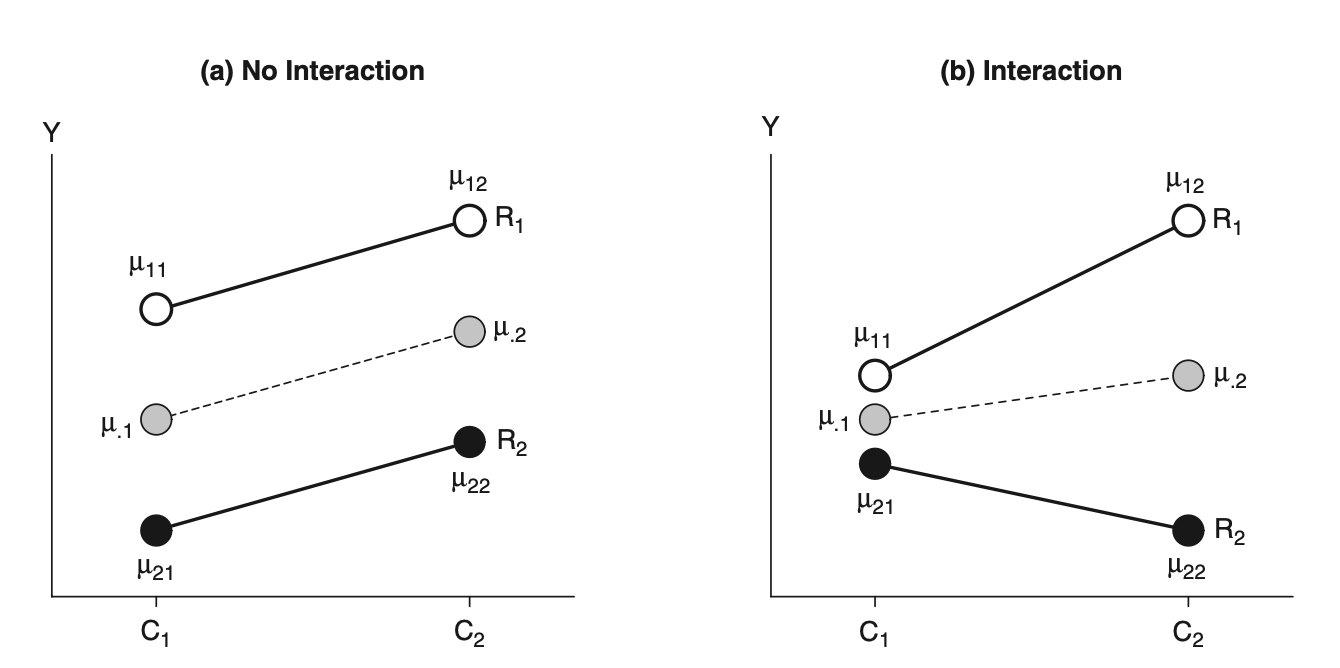
\includegraphics[width=0.9\textwidth]{Lecture25/JF_8_2}
		\caption{
			Interaction in the two-way classification.  In (a), the parallel profiles of means (given by the white and black circles connected by solid lines) indicate that $R$ and $C$ do not interact in affecting $Y$.
			The $R$-effect -- that is, the difference between the two profiles -- is the same at both $C_1$ and $C_2$.
			Likewise, the $C$-effect -- that is , the rise in the line from $C_1$ to $C_2$ -- is the same for both profiles.
			In (b), the $R$-effect differs at the two categories of $C$, and the $C$-effect differs at the two categories of $R$: $R$ and $C$ interact in affecting $Y$.
			In both graphs, the column marginal means $\mu_{\cdot 1}$ and $\mu_{\cdot 2}$ are shown as averages of the cell means in each column (represented by the gray circles connected by broken lines).
			JF Figure 8.2.}
		\label{fig:JF_8_2}
	\end{center}
\end{figure}
%
\subsubsection*{Two-way ANOVA model}
The two-way ANOVA model, suitably defined, provides a convenient means for testing the hypotheses concerning interactions and main effects.
The model is
$$
Y_{ijk} = \mu + \alpha_j + \beta_k + \gamma_{jk} + \epsilon_{ijk}
$$
where $Y_{ijk}$ is the $i$th observation in row $j$, column $k$ of the $RC$ table; $\mu$ is the general mean of $Y$; $\alpha_j$ and $\beta_k$ are the \underline{main-effect} parameters; $\gamma_{jk}$ are \underline{interaction effect} parameters; and $\epsilon_{ijk}$ are errors satisfying the usual linear-model assumptions (i.e.~$\epsilon_{ijk} \distas{iid} \mathcal{N}(0, \sigma^2)$).
By taking expectations, we have
$$
\mu_{jk} \equiv \textit{E}(Y_{ijk}) = \mu + \alpha_j + \beta_k + \gamma_{jk}
$$
We have $r \times c$ population cell means with $1 + r + c + r \times c$ model parameters.
Similar to one-way ANOVA model, we add in additional constraints to make the model identifiable.
$$
\begin{aligned}
	\sum\limits_{j = 1}^ r \alpha_j &= 0\\
	\sum\limits_{k = 1}^c \beta_k &= 0\\
	\sum\limits_{j = 1}^ r \gamma_{jk} &= 0 \quad \mbox{for all } k = 1, \dots, c\\
	\sum\limits_{k = 1}^c \gamma_{jk} &= 0 \quad \mbox{for all } j = 1, \dots, r\\
\end{aligned}
$$
The constraints produce the following solution for model parameters in terms of population cell and marginal means (and we add a hat for their estimates using the sample means):
$$
\begin{aligned}
	\mu &= \mu_{\cdot \cdot}\\
	\alpha_j &= \mu_{j \cdot} - \mu_{\cdot \cdot}\\
	\beta_k &= \mu_{\cdot k} - \mu_{\cdot \cdot} \\
	\gamma_{jk} &= \mu_{jk} - \mu - \alpha_j  - \beta_k \\
	&= \mu_{jk} - \mu_{j\cdot} - \mu_{\cdot k} + \mu_{\cdot \cdot}\\
\end{aligned}
$$

\subsubsection*{Hypotheses with two-way ANOVA}
Some interesting hypotheses:
\begin{enumerate}
	\item Are the cell means all equal? (Equivalent to one-factor ANOVA's ``overall F-test'')\\
	$H_0: \mu_{11} = \mu_{12} = \dots = \mu_{rc}$ vs. $H_a: \mbox{At least two } \mu_{ij} \mbox{ differ}$
	\item Are the marginal means for row main effect equal?\\
	$H_0: \mu_{1\cdot} = \mu_{2\cdot} = \dots = \mu_{r\cdot}$ vs $H_a: \mbox{At least two } \mu_{j\cdot} \mbox{ differ}$\\
	which is equivalent as testing for no row main effects $H_0: \mbox{all } \alpha_j = 0$ (why?)\\
	\begin{pf}
		{\it Answer: }
		This is because $\alpha_j = \mu_{j \cdot} - \mu_{\cdot \cdot}$ such that all $\alpha_j = 0$ is the equivalent as all marginal means are equal $\mu_{1\cdot} = \mu_{2\cdot} = \dots = \mu_{r\cdot}$.
	\end{pf}
	\item Are the marginal means for column main effect equal?\\
	$H_0: \mu_{\cdot 1} = \mu_{\cdot 2} = \dots = \mu_{\cdot c}$ vs $H_a: \mbox{At least two } \mu_{\cdot k} \mbox{ differ}$\\	
	\item Do the factors interact? In other words, does effect of one factor depend on the other factor?
	$H_0: \mu_{ij} = \mu_{\cdot \cdot} + (\mu_{i \cdot} - \mu_{\cdot \cdot}) + (\mu_{\cdot j} - \mu_{\cdot \cdot})$ vs $H_a: \mbox{At least one } \mu_{ij} \neq \mu_{\cdot \cdot} + (\mu_{i \cdot} - \mu_{\cdot \cdot}) + (\mu_{\cdot j} - \mu_{\cdot \cdot})$\\
	The null hypothesis is also equivalent as $H_0: \mbox{all } \gamma_{jk} = 0$.
\end{enumerate}

\subsubsection*{Testing hypotheses in two-way ANOVA}
We follow the notations of JF for incremental sums of squares in ANOVA:
$$
\begin{aligned}
	\textbf{SS}(\gamma | \alpha, \beta) &= \textbf{SS}(\alpha, \beta, \gamma) - \textbf{SS}(\alpha, \beta)\\
	\textbf{SS}(\alpha |  \beta, \gamma) &= \textbf{SS}(\alpha, \beta, \gamma) - \textbf{SS}(\beta, \gamma)\\
	\textbf{SS}(\beta |  \alpha, \gamma) &= \textbf{SS}(\alpha, \beta, \gamma) - \textbf{SS}(\alpha, \gamma)\\
	\textbf{SS}(\alpha | \beta) &= \textbf{SS}(\alpha, \beta) - \textbf{SS}(\beta)\\
	\textbf{SS}(\beta |  \alpha) &=\textbf{SS}(\alpha, \beta) - \textbf{SS}(\alpha)\\
\end{aligned}
$$
where $\textbf{SS}(\alpha, \beta, \gamma)$ denotes the regression sum of squares for the full model which includes both sets of main effects and the interaction. $\textbf{SS}(\alpha, \beta)$ denotes the regression sum of squares for the no-interaction model and $\textbf{SS}(\alpha, \gamma)$ denotes the regression for the model that omits the column main-effect regressors.
Note that the last model violates the principle of marginality because it includes the interaction regressors but omits the column main effects.
However, it is useful for constructing the incremental sum of squares for testing the column main effects.

{\it Additional readings: } \href{http://www.utstat.utoronto.ca/reid/sta442f/2009/typeSS.pdf}{Notes on 3 types of Sum of Squares }by Dr. Nancy Reid.

We now have the two-way ANOVA table
\begin{table}[H]
	\renewcommand{\arraystretch}{1.5}
	\caption{Two-way ANOVA table}
	\label{tab:one_way_anova_table}
	\centering
	\begin{tabular}{lccc}
		\toprule
		Source & Sum of Squares & df &  $H_0$\\
		\hline
		R & $\textbf{SS}(\alpha |  \beta, \gamma)$ & $r - 1$ & all $\alpha_j = 0$\\
		& $\textbf{SS}(\alpha |  \beta)$ & $r - 1$ & all $\alpha_j = 0 \mbox{ } | \mbox{ all } \gamma_{jk} = 0$\\
		\hline
		C & $\textbf{SS}(\beta |  \alpha, \gamma)$ & $c - 1$ & all $\beta_k = 0$\\
		   & $\textbf{SS}(\beta |  \alpha)$ & $c - 1$ & all $\beta_k = 0 \mbox{ } | \mbox{ all } \gamma_{jk} = 0$\\	
		\hline
		RC & $\textbf{SS}(\gamma | \alpha, \beta)$ & (r -1)(c - 1) &  all $\beta_k = 0$\\
		\hline
		Residuals & $\textbf{TSS} - \textbf{SS}(\alpha, \beta, \gamma)$ & n - rc &\\
		\hline
		Total &\textbf{TSS}& n -1 &\\
		\bottomrule
	\end{tabular}
\end{table}
where the residual sum of squares
$$
RSS = \sum\limits_i\sum\limits_j\sum\limits_k(Y_{ijk} - \bar{Y}_{jk})^2
$$

When test for the hypothesis, use the corresponding SS and df together with the residual SS and df to construct the $F$-statistic.
$$
F = \frac{SS/df}{RSS / df_{residual}}
$$
There are two reasonable procedures for testing main-effect hypotheses in two-way ANOVA:
\begin{enumerate}
	\item Tests based on $\textbf{SS}(\alpha | \beta, \gamma)$ and  $\textbf{SS}(\beta | \alpha, \gamma)$  (``type III'' tests) employ models that violate the principle of marginality, but the tests are valid whether or not interactions are present.
	\item Tests based on $\textbf{SS}(\alpha | \beta)$ and $\textbf{SS}(\beta | \alpha)$ (``type II'' tests) conform to the principle of marginality but are valid only if interactions are absent, in which case they are maximally powerful.
\end{enumerate}

Some more jargon:
\begin{itemize}
	\item Experimental unit (EU): entity to which experimental treatment is assigned.\\
	For example, Assign fertilizer treatment to fields.  Fields = EU.
	\item Measurement unit (MU): entity that is measured.\\
	For example, Measure yields at several subplots within each field.  MU: subplot
	\item Treatment structure: describes how different experimental factors are combined to generate treatments.\\
	For example, Fertilizers: A, B, C; Irrigation: High, Low.
	\item Randomization structure: how treatments are assigned to EUs.
	\item Simplest treatment structure: single experimental factor with multiple levels.  Ex. Fertilizers A vs B vs C.
	\item Simplest randomization structure: Completely randomized design -- Experimental treatments assigned to EUs entirely at random.
\end{itemize}

\subsubsection*{Example: Honeybee data}
Entomologist records energy expended ($y$) by $N=27$ honeybees at $a=3$ temperature (A) levels ($20, 30, 40^{\circ}C$) consuming liquids with $b = 3$ levels of sucrose concentration ($B$) ($20\%, 40\%, 60\%$) in a balanced, completely randomized crossed $3 \times 3$ design. 
\begin{table}[H]
	\renewcommand{\arraystretch}{1.5}
	\centering
	\begin{tabular}{cc|ccc}
		\toprule
		Temp & Suc & \multicolumn{3}{c}{Sample}\\
		\hline
		20 & 20 & 3.1 & 3.7 & 4.7\\
		20 & 40 & 5.5 & 6.7 & 7.3\\
		20 & 60 & 7.9 & 9.2 & 9.3\\
		30 & 20 & 6 & 6.9 & 7.5\\
		30 & 40 & 11.5 & 12.9 & 13.4\\
		30 & 60 & 17.5 & 15.8 & 14.7\\
		40 & 20 & 7.7 & 8.3 & 9.5\\
		40 & 40 & 15.7 & 14.3 & 15.9\\
		40 & 60 & 19.1 & 18.0 & 19.9\\
		
		\bottomrule
	\end{tabular}
\end{table}

\begin{enumerate}
	\item What is the experimental unit?\\
	\begin{pf}
		EU = honeybee.
	\end{pf}
	\item What is the treatment structure?\\
	\begin{pf}
		Three levels of temperature (A) are combined with each of the three sucrose concentrations (B).
	\end{pf}
	\item Finish the table below
\begin{table}[H]
	\renewcommand{\arraystretch}{1.5}
	\centering
	\begin{tabular}{lc}
		\toprule
		Source & df\\
		\hline
		A & \\
		B & \\
		$A \times B$ & \\
		Residual & \\
		\hline
		Total &\\
		\bottomrule
	\end{tabular}
\end{table}
{\it Answer: }\\
\begin{pf}
\begin{table}[H]
	\renewcommand{\arraystretch}{1.5}
	\centering
	\begin{tabular}{lr}
		\toprule
		Source & df\\
		\hline
		A & 2\\
		B & 2\\
		$A \times B$ & 4\\
		Residual & 18\\
		\hline
		Total &26\\
		\bottomrule
	\end{tabular}
\end{table}		
\end{pf}
\item 
Consider the model
$$
Y_{ijk} = \mu + \alpha_i + \beta_j + (\alpha \beta)_{ij} + \epsilon_{ijk}
$$
where $i = 1, 2, \dots, a$, $j = 1, 2, \dots, b$ and $k=1, 2, \dots, n$ for a balanced design.\\
Deviation:
\begin{itemize}
	\item total: $y_{ijk} - \bar{y}_{+++}$
	\item due to level $i$ of factor A: $\bar{y}_{i++} - \bar{y}_{+++}$
	\item due to level $j$ of factor B: $\bar{y}_{+j+} - \bar{y}_{+++}$	
	\item due to levels $i$ of factor A and $j$ of factor B after subtracting main effects:
	$$
	\bar{y}_{ij+} - \bar{y}_{+++} - (\bar{y}_{i++} - \bar{y}_{+++}) - (\bar{y}_{+j+} - \bar{y}_{+++}) = \bar{y}_{ij+} - \bar{y}_{i++} - \bar{y}_{+j+} + \bar{y}_{+++}
	$$
\end{itemize}
Use the following equations to calculate the Sum of Squares and fill out the ANOVA table.
$$
\begin{aligned}
SS[Tot] &= \sum\limits_i \sum\limits_j \sum\limits_k (y_{ijk} - \bar{y}_{+++})^2\\
SS[A] &= \sum\limits_i \sum\limits_j \sum\limits_k (\bar{y}_{i++}- \bar{y}_{+++})^2\\
SS[B] &= \sum\limits_i \sum\limits_j \sum\limits_k (\bar{y}_{+j+}- \bar{y}_{+++})^2\\
SS[AB] &= \sum\limits_i \sum\limits_j \sum\limits_k (\bar{y}_{ij+} - \bar{y}_{i++} - \bar{y}_{+j+} + \bar{y}_{+++})^2\\
SS[E] &= \sum\limits_i \sum\limits_j \sum\limits_k (\bar{y}_{ijk}- \bar{y}_{ij+})^2\\
\end{aligned}
$$
where
$$
\begin{aligned}
	\bar{y}_{ij+} &= \frac{1}{n} \sum\limits_k y_{ijk}\\ 
	\bar{y}_{i++} &= \frac{1}{b} \sum\limits_j \bar{y}_{ij+} = \frac{1}{bn} \sum\limits_j \sum\limits_k y_{ijk}\\ 
	\bar{y}_{+j+} &= \frac{1}{a} \sum\limits_i \bar{y}_{ij+}= \frac{1}{an} \sum\limits_i \sum\limits_k y_{ijk}\\ 
	\bar{y}_{+++} &= \frac{1}{a} \sum\limits_i \bar{y}_{i++}= \frac{1}{b} \sum\limits_j \bar{y}_{+j+}\\
	&= \frac{1}{abn} \sum\limits_i \sum\limits_j \sum\limits_k y_{ijk}
\end{aligned}
$$

\begin{table}[H]
	\renewcommand{\arraystretch}{1.5}
	\centering
	\begin{tabular}{lrrrr}
		\toprule
		Source & df & Sum of Squares & Mean Square & F\\
		\hline
		A & & & &\\
		B & & & &\\
		$A \times B$ & & & &\\
		Residual & & & &\\
		\hline
		Total & & & &\\
		\bottomrule
	\end{tabular}
\end{table}
{\it Answer: }\\
\begin{pf}
\begin{table}[H]
	\renewcommand{\arraystretch}{1.5}
	\centering
	\begin{tabular}{lrrrr}
		\toprule
		Source & df & Sum of Squares & Mean Square & F\\
		\hline
		Temp & 2 & 293.16 & 146.58 & 162.00\\
		Suc & 2 & 309.96 & 154.98 &171.28\\
		Temp $\times$ Suc & 4 & 27.13 & 6.78 &7.50\\
		Residual & 18 & 16.29 & 0.90 &\\
		\hline
		Total & 26 & 646.53 & &\\
		\bottomrule
	\end{tabular}
\end{table}	
\end{pf}
\end{enumerate}
%http://www.sthda.com/english/wiki/two-way-anova-test-in-r



















\newpage
\setcounter{section}{27}

\section{Lecture 28: April 5}


\subsection*{Last time}
\begin{itemize}
	\item two-way ANOVA
\end{itemize}


\subsection*{Today}
\begin{itemize}
	\item Announcement: per requested by three students, we will do a third poll on Wednesday for the alternative grading path (the last time).
	\item Lab session review
	\item ANCOVA
	\item Linear contrasts of means
\end{itemize}

\subsubsection*{Additional reference}
\href{https://www4.stat.ncsu.edu/~osborne/st512r/handouts/allpackets.pdf}{Course notes} by Dr. Jason Osborne.

\subsubsection*{A three-factor example}
In a balanced, complete, crossed design, $N=36$ shrimp were randomized to $abc = 12$ treatment combinations from the factors below:
\begin{itemize}
	\item A1: Temperature at $25^{\circ}C$
	\item A2: Temperature at $35^{\circ}C$
	\item B1: Density of shrimp population at $80$ shrimp/40$l$
	\item B2: Density of shrimp population at $160$ shrimp/40$l$
	\item C1: Salinity at $10$ units
	\item C2: Salinity at $25$ units
	\item C3: Salinity at $40$ units
\end{itemize}
The response variable of interest is weight gain $Y_{ijkl}$ after four weeks.

\subsubsection*{Three-way ANOVA model}
$$
\begin{aligned}
Y_{ijkl} &= \mu + \alpha_i + \beta_j + \gamma_k\\
&+ (\alpha \beta)_{ij} + (\alpha \gamma)_{ik} + (\beta \gamma)_{jk}\\
&+ (\alpha\beta \gamma)_{ijk} + \epsilon_{ijkl}\\
\end{aligned}
$$
$$
\begin{aligned}
	i &= 1, 2\\
	j &= 1, 2\\
	k &= 1, 2, 3\\
	l &= 1, 2, 3\\
	\epsilon_{ijkl} &\distas{iid} \mathcal{N}(0, \sigma^2)\\	
\end{aligned}
$$
Many constraints such as (over one dimension):
$$
\begin{aligned}
	\sum\limits_i \alpha_i &= 0\\
	\sum\limits_i (\alpha \beta)_{ij} &= \sum\limits_j (\alpha \beta)_{ij} = 0 \quad \mbox{ for all } i, j\\
	\sum\limits_i (\alpha \beta \gamma)_{ijk} &=  \sum\limits_j (\alpha \beta \gamma)_{ijk} = \sum\limits_k (\alpha \beta \gamma)_{ijk} = 0 \quad \mbox{ for all }i, j, k\\
\end{aligned}
$$

Now, please finish the table below
\begin{table}[H]
	\renewcommand{\arraystretch}{1.5}
	\centering
	\begin{tabular}{lc}
		\toprule
		Source & df\\
		\hline
		A & \\
		B & \\
		C & \\
		$A \times B$ & \\
		$A \times C$ & \\
		$B \times C$ & \\
		$A \times B \times C$ &\\
		Residual & \\
		\hline
		Total &\\
		\bottomrule
	\end{tabular}
\end{table}
{\it Answer: }\\
\begin{pf}
	\begin{table}[H]
		\renewcommand{\arraystretch}{1.5}
		\centering
	\begin{tabular}{lc}
	\toprule
	Source & df\\
	\hline
	A & 1\\
	B & 1\\
	C & 2\\
	$A \times B$ & 1\\
	$A \times C$ & 2\\
	$B \times C$ & 2\\
	$A \times B \times C$ & 2\\
	Residual & 24\\
	\hline
	Total & 35\\
	\bottomrule
\end{tabular}
	\end{table}		
\end{pf}

The three-way ANOVA model includes parameters for
\begin{itemize}
	\item Main effects: $\alpha_i$, $\beta_j$ and $\gamma_k$.
	\item Two-way interactions between each pair of factors: $(\alpha \beta)_{ij}$, $(\alpha \gamma)_{ik}$ and $(\beta \gamma)_{jk}$.
	\item Three-way interaction among all three factors: $(\alpha \beta \gamma)_{ijk}$.
\end{itemize}

Readings:
\begin{enumerate}
	\item JF 8.3.1 on parameter estimates and hypothesis testing for three-way ANOVA model.
	\item JF 8.3.2 on Higher-order classifications.
\end{enumerate}


\subsection*{Analysis of Covariance}
\underline{Analysis of covariance} (ANCOVA) is a term used to describe linear models that contain both qualitative and quantitative explanatory variables.
The method is, therefore, equivalent to dummy-variable regression, discussed in the previous lectures, although the ANCOVA model is parametrized differently from the dummy-regression model.

\underline{Covariate} is a variable known to affect the response that
\begin{enumerate}
	\item differs among EUs
	\item reflects differences that exist independently of experimental treatment.
\end{enumerate}

\subsubsection*{A nutrition example}
A nutrition scientist conducted an experiment to evaluate the effects of four vitamin supplements on the weight gain of laboratory animals.
The experiment was conducted in a completely randomized design with $N=20$ animals randomized to $a=4$ supplement groups, 
each with sample size $n \equiv 5$.
The response variable of interest is weight gain, but calorie intake $z$ was measured simultaneously.
\begin{table}[H]
	\renewcommand{\arraystretch}{1.5}
	\centering
	\begin{tabular}{|cc|cc|cc|cc|}
		\toprule
		Diet & $y(g)$ & Diet & $y$& Diet & $y$& Diet & $y$\\
		\hline
		1 & 48 & 2 & 65 & 3 & 79 & 4 &59 \\
		1 & 67 & 2 & 49 & 3 & 52 & 4 &50 \\
		1 & 78 & 2 & 37 & 3 & 63 & 4 &59 \\
		1 & 69 & 2 & 75 & 3 & 65 & 4 &42 \\
		1 & 53 & 2 & 63 & 3 & 67 & 4 &34 \\
		\hline
		1 & $\bar{y}_{1+} = 63$ & 2 & $\bar{y}_{2+} = 57.8$ & 3 & $\bar{y}_{3+} = 65.2$ & 4 &$\bar{y}_{4+} = 48.8$ \\
		1 & $s_1 = 12.3$ & 2 & $s_2 = 14.9$ & 3 & $s_3 = 9.7$ & 4 &$s_4 = 10.9$ \\
		\bottomrule
	\end{tabular}
\end{table}

Question: Is there evidence of a vitamin supplement effect?

\begin{table}[H]
	\renewcommand{\arraystretch}{1.5}
	\centering
	\begin{tabular}{lrrrrr}
		& Df & Sum Sq & Mean Sq & F value & Pr($>$F)\\
	Diet & 3 & 	797.8  & 265.9 &  1.823 & 0.184\\
	Residuals  & 16& 2334.4 &  145.9 & &\\              	
	\end{tabular}
\end{table}
\begin{pf}
Conclusion: at $\alpha = 0.05$ level, there is no significant difference between vitamin supplement levels on weight gain.
\end{pf}

But calorie intake $z$ was measured simultaneously:
\begin{table}[H]
	\renewcommand{\arraystretch}{1.5}
	\centering
	\begin{tabular}{ccc|ccc|ccc|ccc}
		\toprule
		Diet & $y(g)$ & $z$ & Diet & $y$ & $z$& Diet & $y$ & $z$& Diet & $y$ & $z$\\
		\hline
		1 & 48 & 350 & 2 & 65 & 400 & 3 & 79 & 510 & 4 & 59 & 530\\
		1 & 67 & 440 & 2 & 49 & 450 & 3 & 52 & 410 & 4 & 50 & 520\\
		1 & 78 & 440 & 2 & 37 & 370 & 3 & 63 & 470 & 4 & 59 & 520\\
		1 & 69 & 510 & 2 & 75 & 530 & 3 & 65 & 470 & 4 & 42 & 510\\
		1 & 53 & 470 & 2 & 63 & 420 & 3 & 67 & 480 & 4 & 34 & 430\\						
		\bottomrule
	\end{tabular}
\end{table}

Question: How and why could these new data be incorporated into analysis?\\
Answer: ANCOVA can be used to reduce unexplained variation.

ANCOVA model, 
$$
y_{ij} = \mu + \alpha_i + \beta z_{ij} + \epsilon_{ij}
$$
where $\mu$ is the reference level, $\alpha_i$ is the main effect of treatment, $\beta$ is the partial regression coefficient, 
and $\epsilon_{ij} \distas{iid} \mathcal{N}(0, \sigma^2)$.
The model is equivalent as the dummy-variable regression model,
$$
Y_i = \beta_0 + \beta_1 x_{i1} + \beta_2 x_{i2} + \beta_3 x_{i3} + \beta_z z_i + \epsilon_i \quad \mbox{ for } i = 1, \dots, 20
$$

Finish the table below
\begin{table}[H]
	\renewcommand{\arraystretch}{1.5}
	\centering
	\begin{tabular}{lr}
		\toprule
		Source & df\\
		\hline
		Diet & \\
		Covariate & 1\\
		Residual & \\
		\hline
		Total &\\
		\bottomrule
	\end{tabular}
\end{table}
{\it Answer: }\\
\begin{pf}
\begin{table}[H]
	\renewcommand{\arraystretch}{1.5}
	\centering
	\begin{tabular}{lr}
		\toprule
		Source & df\\
		\hline
		Diet & 3\\
		Covariate & 1\\
		Residual & 15\\
		\hline
		Total & 19\\
		\bottomrule
	\end{tabular}
\end{table}
\end{pf}

To test for difference among treatments.
The null hypothesis in terms of $\alpha_i$ is\\
$H_0: \alpha_1 = \alpha_2  = \dots = \alpha_4 = 0$ v.s. $H_a: \mbox{ at least one } \alpha_i \ne 0$\\
And the null hypothesis in terms of $\beta_i$ is\\
$H_0: \beta_1 = \beta_2  = \beta_3 = 0$ v.s. $H_a: \mbox{ at least one } \beta_i \ne 0$

Question: which two models do we compare when testing the above null hypothesis?
{\it Answer: }\\
\begin{pf}
\begin{itemize}
	\item In terms of ANOVA and ANCOVA models, we compare the one-way ``ANOVA'' model (actually the simple linear regression model) with only the covariate term to the ANCOVA model that has both the covariate and the treatment.\\
	\colorbox{shadecolor}{aov(y $\sim$ z, data = vitamin.supplement)} vs \colorbox{shadecolor}{aov(y $\sim$ Diet + z, data = vitamin.supplement)} 
	\item In terms of the dummy-variable regression model, we compare the simple linear regression model of regression $y$ on $z$ to the model that includes the dummy-variable for Diet (treatments).\\
	\colorbox{shadecolor}{lm(y $\sim$ z, data = vitamin.supplement)} vs \colorbox{shadecolor}{lm(y $\sim$ Diet + z, data = vitamin.supplement)} 
\end{itemize}
\end{pf}

\subsection*{Linear contrasts of means}
With ANOVA (or ANCOVA) models, we do not generally test hypotheses about individual coefficients (but we can do so if we wish).
For dummy-coded regressors in one-way ANOVA, a $t$-test or $F$-test of $H_0: \alpha_1 = 0$, for example, is equivalent to testing for the difference in means between the first group and the baseline group, $H_0: \mu_1 = \mu_m$.

Consider the one-way ANOVA model:
$$
Y_{ij} = \mu_i + \epsilon_{ij}, i = 1, 2, \dots, t, \mbox{ and } j = 1, 2, \dots, n_i
$$
with $\epsilon_{ij} \distas{iid} \mathcal{N}(0, \sigma^2)$.

A linear function of the group means of the form
$$
\theta = c_1 \mu_1 + c_2 \mu_2 + \dots + c_t \mu_t
$$
is called a \underline{linear combination} of the treatment means.
And the $c_i$'s are the \underline{coefficients} of the linear combination.
If
$$
c_1 + c_2 + \dots + c_t = \sum\limits_{j = 1}^t c_j = 0,
$$
the linear combination is called a \underline{contrast}.
Contrasts with more than two non-zero coefficients are called \underline{complex contrasts}.

Let two contrasts $\theta_1$ and $\theta_2$ be given by
$$
\begin{aligned}
	\theta_1 &= c_1 \mu_1 + \dots + c_t \mu_t = \sum\limits_{j = 1}^t c_j \mu_j\\
	\theta_2 &= d_1 \mu_1 + \dots + d_t \mu_t = \sum\limits_{j = 1}^t d_j \mu_j,\\	
\end{aligned}
$$
then the two contrasts $\theta_1$ and $\theta_2$ are \underline{mutually orthogonal} if the products of their coefficients sum to zero:
$$
c_1 d_1 + \dots + c_t d_t = \sum\limits_{j=1}^t c_j d_j = 0
$$

$\theta_i$ and $\theta_j$ are orthogonal $\implies$ $\hat{\theta}_i$ and $\hat{\theta}_j$ are statistically independent.

\subsubsection*{Types of effects}
Consider the following two-way ANOVA model:
$$
\begin{aligned}
Y_{ijk} &= \mu + \alpha_i + \beta_j + (\alpha \beta)_{ij} + \epsilon_{ijk}\\
i &= 1, 2 = a \mbox{ and } j = 1, 2=b \mbox{ and } k = 1, 2, \dots , 7 = n.\\
\end{aligned}
$$
$\epsilon_{ijk} \distas{iid} \mathcal{N}(0, \sigma^2)$.  Parameter constraints: $\sum_i \alpha_i = \sum_j \beta_j = 0$ and 
$\sum_i (\alpha \beta)_{ij} = 0$ for each $j$ and $\sum_j (\alpha \beta)_{ij} = 0$ for each $i$.
\begin{itemize}
	\item Factor A: AGE has $a = 2$ levels - $A_1: $ younger and $A_2: $ older
	\item Factor B: GENDER has $b = 2$ levels - $B_1: $ female and $B_2: $ male
\end{itemize}

Three kinds of effects in this $2 \times 2$ design:
\begin{enumerate}
	\item \underline{Simple effects} are simple contrasts.
	    \begin{itemize}
	    	\item $\mu(A_1 B) = \mu_{12} - \mu_{11}$ - simple effect of gender for young folks.
	    	\item $\mu(A B_1) = \mu_{21} - \mu_{11}$ - simple effect of age for women. 
	    \end{itemize}
    \item \underline{Interaction effects} are differences of simple effects:
    $\mu(AB) = \mu(AB_2) - \mu(AB_1) = (\mu_{22} - \mu_{12}) - (\mu_{21} - \mu_{11})$
    \begin{itemize}
    	\item difference between simple age effects for men and women
    	\item difference between simple gender effects for old and young folks
    	\item interaction effect of AGE and GENDER.
    \end{itemize}
    \item \underline{Main effects} are averages or sums of simple effects
    $$
    \begin{aligned}
    	\mu(A) &= \frac{1}{2} (\mu(AB_1) + \mu(AB_2))\\
    	\mu(B) &= \frac{1}{2} (\mu(A_1 B) + \mu(A_2B))\\    	
    \end{aligned}
    $$
\end{enumerate}








\newpage
\setcounter{section}{28}

\section{Lecture 29: April 7}


\subsection*{Last time}
\begin{itemize}
	\item ANCOVA
	\item Linear contrasts of means
\end{itemize}


\subsection*{Today}
\begin{itemize}
	\item One last poll on alternative grading path
	\begin{itemize}
		\item Consider the votes on the three polls (including today's), if we model them as binomial distributed random variables with probability for `yes' as $p_1$, $p_2$ and $p_3$
		\item What is the likelihood function?
		\item How do we test the null hypothesis of $H_0: p_1 = p_2 = p_3$?
		\item What do you expect?  Why?
	\end{itemize}
	\item Final exam will be posted on April 30th (per requested by Grace), Due May 11th 11:59pm
	\item Sampling distribution of linear contrasts
	\item Multiple comparisons
	\item Sample size computations for one-way ANOVA	
	\item Lack of fit test	
%	\item One-way random effect model (JF Chapter 23 + Dr. Osborne's notes)
\end{itemize}

\subsubsection*{Additional reference}
\href{https://www4.stat.ncsu.edu/~osborne/st512r/handouts/allpackets.pdf}{Course notes} by Dr. Jason Osborne.

\subsection*{Sampling distribution of linear contrast estimates}
For a linear contrast
$$
\theta = c_1 \mu_1 + \dots + c_t \mu_t
$$
The {\it best} estimator for a contrast of interest can be obtained by substituting treatment group sample means $\bar{y}_{i+}$ for treatment population means $\mu_i$ in the contrast $\theta$:
$$
\hat{\theta} = c_1 \bar{Y}_{1+} + c_2 \bar{Y}_{2+} + \dots + c_t \bar{Y}_{t+}
$$

\subsubsection*{Example}
Recall the binding fraction data that investigate binding fraction for several antibiotics using $n = 20$ bovine serum samples:
\begin{table}[H]
	\centering
	\begin{tabular}{c|c|c}
		\toprule
		Antibiotic & Binding Percentage & Sample mean \\
		\hline
		Penicillin G & 29.6 24.3 28.5 32.0 & 28.6\\
		Tetracyclin & 27.3 32.6 30.8 34.8 & 31.4\\
		Streptomycin & 5.8 6.2 11.0 8.3 & 7.8\\
		Erythromycin & 21.6 17.4 18.3 19 & 19.1\\
		Chloramphenicol & 29.2 32.8 25.0 24.2&27.8\\
		\bottomrule
	\end{tabular}
\end{table}

Consider the pairwise contrast comparing penicillin (population) mean to Tetracyclin mean:
$$
\theta = \mu_1 - \mu_2 = (1) \mu_1 + (-1) \mu_2 + (0) \mu_3 + (0) \mu_4 + (0) \mu_5
$$
Obtain a point estimator of $\theta$.\\
{\it Answers:}\\
\begin{pf}
	$$
	\begin{aligned}
		\hat{\theta} &= \hat{\mu}_1 - \hat{\mu}_2 = \bar{Y}_{1+} - \bar{Y}_{2+}\\
		&= 28.6 - 31.4 = -2.8\\
	\end{aligned}
	$$
\end{pf}

Question: How good is this estimate?  In other words, how much uncertainty associated with the estimate?

We want to characterize the sampling distribution of $\hat{\theta}$.
According to our model setup, $Y_{ij}$ follow normal distributions.
$\hat{\theta}$ is a linear function of $Y_{ij}$, so that $\hat{\theta}$ follows a normal distribution.
We want to derive the mean and variance (the two sufficient statistics) to characterize the normal distribution that $\hat{\theta}$ follows:
$$
\hat{\theta} \sim \mathcal{N}(\theta, Var(\hat{\theta}))
$$

{\it Derive expressions for the mean and the variance:}\\
\begin{pf}
	For the mean, we have
	$$
	\begin{aligned}
E(\hat{\theta}) &= E(\hat{\mu}_1) - E(\hat{\mu}_2) = E(\bar{Y}_{1+}) - E(\bar{Y}_{2+})\\
&= \mu_1 - \mu_2 = \theta \\
	\end{aligned}
	$$
	The variance follows
	$$
	\begin{aligned}
		Var(\hat{\theta}) &= Var(\sum\limits_j c_j \bar{Y}_{j+})\\
		&= \sum\limits_j Var(c_j \bar{Y}_{j+})\\
		&= \sum\limits_j c_j^2 Var(\bar{Y}_{j+})\\
		&= \sum\limits_j  \frac{c_j^2}{n_j} \sigma^2
	\end{aligned}
	$$
\end{pf}

Therefore, the standard error:
$$
SE(\hat{\theta}) = \sqrt{Var(\hat{\theta})} = \sqrt{\sigma^2 \sum\limits_{j = 1}^t \frac{c_j^2}{n_j}}
$$
which is estimated by
$$
\reallywidehat{SE}(\hat{\theta}) = \sqrt{MS[E] \sum\limits_{j = 1}^t \frac{c_j^2}{n_j}}
$$

To test $H_0: \theta =\theta_0$ (often $0$) versus $H_1: \theta \ne \theta_0$, use $t$-test:
$$
t = \frac{\hat{\theta} - \theta_0}{\reallywidehat{SE}(\hat{\theta})} \distas{H_0} t_{N-t}
$$
At level $\alpha$, the critical value for this test is $t(N - t, \alpha/2)$
and $100(1 - \alpha)\%$ confidence interval for a contrast $\theta = \sum c_j \mu_j$ is given by
$$
\sum c_j \bar{Y}_{j+} \pm t(N - t, \alpha /2)\sqrt{MS[E] \sum \frac{c_j^2}{n_j}}
$$


\subsection*{Multiple Comparisons}
Let's first review type I and type II errors.
\begin{table}[H]
	\renewcommand{\arraystretch}{1.5}
	\centering
	\begin{tabular}{c|c|c}
		\toprule
		& $H_0$ is True & $H_0$ is False\\
		\hline
		Don't reject $H_0$ & Probability $1 - \alpha$ & Probability $\beta$\\
		Reject $H_0$ & Probability $\alpha$ & Probability $1 - \beta$\\
		\bottomrule
	\end{tabular}
\end{table}
\begin{itemize}
	\item Type I error: rejection of a true null hypothesis (false positive).
	\item Type II error: failure to reject a false null hypothesis (false negative).
	\item Type I error rate or significance level ($\alpha$): the probability of rejecting the null hypothesis given the null hypothesis is true.
	\item Type II error rate ($\beta$): the probability of failure to reject the null hypothesis given the null hypothesis is false.  $1 - \beta$ gives the power of a test.
\end{itemize}

Now, let's consider all simple (pairwise) contrasts for the binding fraction data with $t=5$ antibiotic treatments of the form $\theta = \mu_i - \mu_j$.
\begin{itemize}
	\item We have $\left( \begin{array}{c}
		5\\ 2\\
	\end{array} \right) = 10$ tests for significance each at level $\alpha = 0.05$
	\item what is the probability of committing at least one type I error?
	    \begin{pf}
	    	$$
	    	1 - (1 - \alpha)^{10}
	    	$$
	    \end{pf}
\end{itemize}

We need to consider the \underline{familywise error rate} (fwe) when testing $k$ contrasts:
$$
fwe = \Pr(\mbox{at least one type I error})
$$
Methods for simultaneous inference for multiple contrasts include
\begin{itemize}
	\item Bonferroni
	\item Scheff\'e
	\item Tukey
\end{itemize}

When the number of comparisons is in the hundreds or thousands (e.g.~genome-wide association studies), and FWE control is hopeless, more manageable type I error rate is the \underline{False Discovery Rate (FDR)}:
$$
FDR = \textit{E}(\frac{\mbox{Falsely rejected null hypotheses}}{\mbox{Number of rejected null hypotheses}})
$$

\subsubsection*{Bonferroni correction}
Suppose interest lies in exactly $k$ contrasts.
The Bonferroni adjustment to $\alpha$ controls $fwe$ is
$$
\alpha_{bonferroni} = \frac{\alpha}{k}
$$
and simultaneous $95\%$ confidence intervals for the $k$ contrasts are given by
$$
\begin{aligned}
	a_1 \bar{Y}_{1+} + \dots + a_t \bar{Y}_{t+} &\pm t(\frac{\alpha_{bonferroni}}{2}, \nu) \sqrt{MS[E]\sum \frac{a_j^2}{n_j}}\\
	b_1 \bar{Y}_{1+} + \dots + b_t \bar{Y}_{t+} &\pm t(\frac{\alpha_{bonferroni}}{2}, \nu) \sqrt{MS[E]\sum \frac{b_j^2}{n_j}}\\	
	&\dots\\
	k_1 \bar{Y}_{1+} + \dots + k_t \bar{Y}_{t+} &\pm t(\frac{\alpha_{bonferroni}}{2}, \nu) \sqrt{MS[E]\sum \frac{k_j^2}{n_j}}\\
\end{aligned}
$$
where $\nu$ denotes $df$ for error.

{\it Example: } for the binding fraction example, consider only pairwise comparisons with Penicillin:
$$
\theta_1 = \mu_1 - \mu_2, \theta_2 = \mu_1 - \mu_3, \theta_3 = \mu_1  - \mu_4, \theta_4 = \mu_1 - \mu_5
$$
We have $k=4, \alpha_{bonferroni} = 0.05/k = 0.0125$ and $t(\frac{\alpha_{bonferroni}}{2}, 15) = 2.84$.
Substitution leads to
$$
\begin{aligned}
&t(\frac{\alpha_{bonferroni}}{2}, 15)\sqrt{MS[E]\left( \frac{1^2}{4} + \frac{(-1)^2}{4} + \frac{0^2}{4} + \dots + \frac{0^2}{4}\right)}\\
=& 2.84 \sqrt{(9.05)\frac{2}{4}} = 6.0\\
\end{aligned}
$$
so that {\bf simultaneous} $95\%$ confidence intervals for $\theta_1$, $\theta_2$, $\theta_3$ and $\theta_4$ take the form
$$
\bar{y}_{1+} - \bar{y}_{i+} \pm 6.0
$$

\subsubsection*{Scheff\'e}
Another method to construct {\bf simultaneous} $95\%$ confidence intervals for {\bf ALL} contrasts, use
$$
\sum\limits_{j = 1}^t c_j \bar{y}_{j+} \pm \sqrt{(t - 1)(F^*)MS[E]\sum\limits_{j = 1}^t \frac{c_j^2}{n_j}}
$$
where $F^* = F(\alpha, t - 1, N - t)$.  For a pairwise comparisons of means, $\mu_j$ and $\mu_k$, this yields
$$
\bar{y}_{j+} - \bar{y}_{k+} \pm \sqrt{(t - 1)(F^*)MS[E](1 / n_j + 1 / n_k)}
$$
Using $\alpha = 0.05$, need to specify
\begin{itemize}
	\item $t$ (from the design)
	\item $F^*$ (same critical value as for $H_0: \alpha_i \equiv 0$).
	\item $MS[E]$ (from the data)
	\item $\bar{y}_{j+}$, $\bar{y}_{k+}$
	\item $n_j$, $n_k$ (from the data)
\end{itemize}
For binding fraction data,
$$
\sqrt{(t - 1)(F^*)MS[E](\frac{1}{n_j} + \frac{1}{n_k})} = \sqrt{(5 - 1)(3.06)9.05(\frac{1}{4} + \frac{1}{4})} = 7.44
$$
If any two sample means differ by more than $7.44$, they differ significantly.

\subsubsection*{Tukey}
Tukey's method is better than Scheff\'e's method when making {\bf all pairwise} comparisons in balanced designs ($n = n_1 = n_2 = \dots =n_t$).
It is conservative, controlling the experimentwise error rate, and has a lower type II error rate in these cases than Scheff\'e.  (It is more powerful.)

For simple contrasts of the form
$$
\theta = \mu_j - \mu_k
$$
to test
$$
H_0: \theta = 0 \mbox{ vs } H_1: \theta \ne 0
$$
reject $H_0$ at level $\alpha$ if
$$
|\hat{\theta}| > q(t, N-t, \alpha)\sqrt{\frac{MS[E]}{n}}
$$
where $q(t, N-t, \alpha)$ denotes $\alpha$ level \underline{studentized range} for $t$ means and $N-t$ degrees of freedom,
the quantity $q(t, N-t, \alpha)\sqrt{\frac{MS[E]}{n}}$ is referred to as \underline{Tukey's honestly significant difference (HSD)}.
The studentized ranges can be calculated using R function \colorbox{shadecolor}{qtukey($1 - \alpha$, $t$, $N-t$)}. 













\newpage
\setcounter{section}{30}

\section{Lecture 31: April 12}


\subsection*{Last time}
\begin{itemize}
	\item One last poll on alternative grading path
	\item Sampling distribution of linear contrasts
	\item Multiple comparisons
\end{itemize}


\subsection*{Today}
\begin{itemize}
	\item {\bf Last} poll on alternative grading path result: {\it passed} with $4 + 4$ yes, $4 + 1$ no ($0$ by emails...?)
	\item Sample size computations for one-way ANOVA	
	\item Lack of fit test	
	\item One-way random effect model (JF Chapter 23 + Dr. Osborne's notes)
\end{itemize}

\subsubsection*{Additional reference}
\href{https://www4.stat.ncsu.edu/~osborne/st512r/handouts/allpackets.pdf}{Course notes} by Dr. Jason Osborne.

\subsection*{Sample size computations for one-way ANOVA}

Now consider the null hypothesis in a balanced experiment using one-way ANOVA to compare $t$ treatment means and $\alpha=0.05$:
$$
H_0: \mu_1 = \mu_2 = \dots = \mu_t = \mu
$$
versus the alternative
$$
H_a: \mu_i \ne \mu_j \mbox{ for some } i\ne j
$$
Suppose that we intend to use a balanced design.  How big does our sample size $n_1 = n_2 = \dots = n_t = n$ need to be?

The answer depends on lots of things, namely, $\sigma^2$ and how many treatment groups $t$ and how much of a difference among the means we hope to be able to detect, and with how big a probability.

Given $\alpha$, $\mu_1, \dots, \mu_t$ and $\sigma^2$, we can choose $n$ to ensure a power of at least $\beta$ (i.e.~type II error rate) using the \underline{noncentral F distribution}.

Recall that the critical region for the statistic $F = MS[Trt]/MS[E]$ is everything bigger than $F(\alpha, t- 1, N - t) = F^*$.

The power of the $F$-test conducted using $\alpha = 0.05$ to reject $H_0$ under this alternative is given by
\begin{equation}
1 - \beta = \Pr(MS[Trt]/MS[E]>F^*; H_1 \mbox{ is true}).
\label{eq:power}
\end{equation}

Let $\tau_i = \mu_i - \mu$ for each treatment $i$ so that
$$
H_0: \tau_1 = \tau_2 = \dots = \tau_t = 0
$$
When some $H_1$ is true and the sample size $n$ is used in each group, it can be shown that the $F$ ratio has the noncentral $F$ distribution with noncentrality parameter
$$
\gamma = \sum\limits_{j = 1}^t n_j \left(\frac{\tau_j}{\sigma}\right)^2 = n\sum\limits_{j = 1}^t \left(\frac{\tau_j}{\sigma}\right)^2
$$
This is the parameterization for the $F$ distribution used in both SAS and R.

One way to obtain an adequate sample size is trial and error.
Software packages can be used to get probabilities of the form~\ref{eq:power} for various values of $n$.

\subsubsection*{Example}
Suppose we want to test equal mean binding fractions among antibiotics against the alternative
$$
H_1:\mu_P = \mu + 3, \mu_T = \mu + 3, \mu_S = \mu - 6, \mu_E = \mu, \mu_C = \mu
$$
so that 
$$
\tau_1 = \tau_2 = 3, \tau_3 = -6, \tau_4 = \tau_5 = 0.
$$
Assume $\sigma = 3$ (is it arbitrary? any idea of how to guess?) and we need to use $\alpha = 0.05$.
The noncentrality parameter is given by
$$
\gamma = n[(\frac{3}{3})^2 + (\frac{3}{3})^2 + (\frac{-6}{3})^2]
$$
The $\alpha = 0.05$ critical value for $H_0$ is given by
$$
F^* = F(5 - 1, 5n - 5, 0.05).
$$
We need the area to the right of $F^*$ for the noncentral $F$ distribution with degrees of freedom $4$ and $5(n - 1)$ and noncentrality parameter $\gamma = 6n$ to be greater or equal to the desired power level of $1 - \beta = 0.8$.

We will revisit this example in the lab session on Friday.

\subsection*{Lack-of-fit test}

Hiking example: completely randomized experiment involving alpine meadows in the White Mountains of New Hampshire.
$N = 20$ lanes of dimension $0.5m \times 1.5m$ randomized to $5$ trampling treatments:
\begin{table}[H]
	\renewcommand{\arraystretch}{1.5}
	\centering
	\begin{tabular}{c|c|cccc}
		\toprule
		$i$: trt group & $x$: Number of passes & \multicolumn{4}{c}{$y_{ij}$: Height (cm)}\\
		\hline
		1 & 0 & 20.7 & 15.9 & 17.8 & 17.6\\
		2 & 25 & 12.9 & 13.4 & 12.7 & 9.0\\
		3 & 75 & 11.8 & 12.6 & 11.4 & 12.1\\
		4 & 200 & 7.6 & 9.5 & 9.9 & 9.0\\
		5 & 500 & 7.8 & 9.0 & 8.5 & 6.7\\								
		\bottomrule
	\end{tabular}
\end{table}

Two models for mean plant height:
$$
\begin{aligned}
	\mbox{SLR model: }& \mu(x) = \beta_0 + \beta_1 x\\
	\mbox{one-factor ANOVA model: }& \mu_{ij} = \mu + \alpha_i\\
\end{aligned}
$$
When the $t$ treatments have an interval scale, the SLR model, and all polynomials of degree $p\le t-2$ (why?), are nested in one-factor ANOVA model with $t$ treatment means.

{\it Answer: }\\
\begin{pf}
	For t levels, there are $t - 1$ degrees of freedom.  A polynomial model of degree $p$ has $p + 1$ number of parameters (in other words, takes $p+1$ degrees of freedom).
\end{pf}

\subsubsection*{F-ratio for lack-of-fit test}
To test for lack-of-fit of a polynomial (reduced) model of degree $p$, use extra sum-of-squares $F$-ratio on $t - 1 - p$ and $N - t$ df:
$$
F = \frac{SS[\mbox{lack of fit}]/(t - 1 - p)}{MS[\mbox{pure error}]}
$$
where
$$
MS[\mbox{pure error}] = MS[E]_{full}
$$
and
$$
\begin{aligned}
	SS[\mbox{lack-of-fit}] &= SS[Trt] - SS[Reg]_{poly}\\
	&= SS[E]_{poly} - SS[E]_{full}\\
\end{aligned}
$$
What is the $SS[\mbox{lack of fit}]$ for the meadows data?
\begin{pf}
	In a simple linear ($p=1$) model for the meadows data,
$$
SS[\mbox{lack-of-fit}] = 243.163 - 141.295 = 101.867 \quad \mbox{ on } t- 1 - p = 3 \mbox{ df}
$$
and the sum of squares for the full model is $SS[E]_{full} = 30.93$ that leads to
$$
F = \frac{101.867/3}{30.93/15} \approx \frac{34}{2.1} = 16.5
$$
(highly significant since $F(0.01, 3, 15) = 5.42$.)
$\Rightarrow$ model misspecified: SLR model suffers from lack of fit.
\end{pf}

Next step: either go with the one-factor ANOVA model or specify some other model, such as quadratic.


\subsection*{One-way random effects model}

Let's first consider an example.
\begin{itemize}
	\item Genetics study w/ beef animals.  Measure birthweight $Y$ (lbs).
	\item $t = 5$ sires, each mated to a separate group of $n = 8$ dams.
	\item $N=40$, completely randomized.
\end{itemize}
\begin{table}[H]
	\renewcommand{\arraystretch}{1.5}
	\centering
	\begin{tabular}{cc|cccccccc|c|c}
		\toprule
		Sire \# & Level & \multicolumn{8}{c}{Sample Birthweights} & $\bar{y}_{i+}$ & $s_i$\\
		\hline
		177 & 1 & 61 & 100 &56 & 113 & 99 & 103 & 75 & 62 & 83.6 & 22.6\\
		200 & 2 & 75 & 102 &95 & 103 & 98 & 115 & 98 & 94 & 97.5 & 11.2\\
		201 & 3 & 58 & 60 &60 & 57 & 57 & 59 & 54 & 100 & 63.1 & 15.0\\
		202 & 4 & 57 & 56 &67 & 59 & 58 & 121 & 101 & 101 & 77.5 & 25.9\\
		203 & 5 & 59 & 46 &120 & 115 & 115 & 93 & 105 & 75 & 91.0 & 28.0\\								
		\bottomrule
	\end{tabular}
\end{table}

Question: Statistical model for these data?\\
Answer: One-way fixed effects model?
$$
Y_{ij} = \mu + \tau_i + \epsilon_{ij}
$$
where $\tau_i$ denotes the difference between the mean birthweight of population of offspring from sire $i$ and $\mu$, mean of whole population.

\underline{The one-way random effects model}
$$
Y_{ij} = \underbrace{\mu}_{\mbox{fixed}} + \underbrace{T_i}_{\mbox{random}} + \underbrace{\epsilon_{ij}}_{\mbox{random}}  \quad \mbox{ for } i = 1, 2, \dots, t \mbox{ and }  j = 1, \dots, n
$$
with
\begin{itemize}
	\item $T_1, T_2, \dots, T_t \distas{iid} \mathcal{N}(0, \sigma_T^2)$
	\item $\epsilon_{11}, \dots, \epsilon_{tn} \distas{iid} \mathcal{N}(0, \sigma^2)$
	\item $T_1, T_2, \dots, T_t$ independent of $\epsilon_{11},, \dots, \epsilon_{tn}$
\end{itemize}

Features
\begin{itemize}
	\item $T_1, T_2, \dots$ denote \underline{random effects}, drawn from some population of interest.  That is $T_1, T_2, \dots$ is a \underline{random sample}.
	\item $\sigma_T^2$ and $\sigma^2$ are called \underline{variance components}
	\item conceptually different from one-way fixed effects model
\end{itemize}

For beef animal genetic study, with $t = 5$ and $n = 8$, the random effects $T_1, T_2, \dots, T_5$ reflect sire-to-sire variability.

No particular interest in $\tau_1, \tau_2, \dots, \tau_5$ from the fixed effects model:
$$
Y_{ij} = \underbrace{\mu}_{\mbox{fixed}} + \underbrace{\tau_i}_{\mbox{fixed}} + \underbrace{\epsilon_{ij}}_{\mbox{random}}  \quad \mbox{ for } i = 1, 2, \dots, t \mbox{ and }  j = 1, \dots, n
$$
with
\begin{itemize}
	\item $\tau_1, \tau_2, \dots, \tau_t$ unknown model parameters
	\item $\epsilon_{11}, \dots, \epsilon_{tn} \distas{iid} \mathcal{N}(0, \sigma^2)$
\end{itemize}

\subsubsection*{Exercise}
Using the random effects model, specify
$$
\textit{E}(Y_{ij}) \mbox{ and } \textit{Var}(Y_{ij})
$$
Recall:
\begin{itemize}
	\item Two {\it components} to variability in data: $\sigma^2$, $\sigma_T^2$
	\item $T_1, T_2, \dots, T_5$ a random sample of sire effects
	\item Sire effects is a population in its own right.
	\item Model parameters: $\sigma^2$, $\sigma_T^2$, $\mu$.
\end{itemize}

{\it Answer:}\\
\begin{pf}
$$
\textit{E}(Y_{ij}) = \textit{E}(\mu) + \textit{E}(T_i) + \textit{E}(\epsilon_{ij})  = \mu
$$
$$
\textit{Var}(Y_{ij}) = \textit{Var}(\mu + T_i + \epsilon_{ij}) = \textit{Var}(T_i) + \textit{Var}(\epsilon_{ij}) = \sigma_T^2 + \sigma^2
$$
\end{pf}

Sums of squares and mean squares are the same as in one-way fixed effects ANOVA:
$$
\begin{aligned}
	SS[T] &= \sum\sum(\bar{y}_{i+} - \bar{y}_{++})^2\\
	SS[E] &= \sum\sum({y}_{ij} - \bar{y}_{i+})^2\\
	SS[Tot] &= \sum\sum({y}_{ij} - \bar{y}_{++})^2\\
\end{aligned}
$$

\subsubsection*{ANOVA table}
The ANOVA table is almost the same, it just has a different expected mean squares column:
\begin{table}[H]
	\renewcommand{\arraystretch}{1.5}
	\centering
	\begin{tabular}{ccccc}
		\toprule
		Source & SS & df & MS & Expected MS \\
		\hline
		Treatment & $SS[T]$ & $t - 1$ & $MS[T]$ & $\sigma^2 + n\sigma^2_T$\\
		Error & $SS[E]$ & $N - t$ & $MS[E]$ & $\sigma^2$\\
		Total & $SS[Tot]$ & $N - 1$ &  &\\
		\bottomrule
	\end{tabular}
\end{table}

\subsubsection*{Estimating parameters of one-way random effects model}
\begin{enumerate}
	\item {\bf Method of moment (M.o.M.) estimation}: Equate EMS with observed MS and solve. Problem: M.o.M estimation can give $\hat{\sigma}^2 < 0$ (estimates of variances $<0$)
	\item {\bf Maximum likelihood (ML) / Restricted maximum likelihood (REML)}: Numerical procedures that avoid negative variance estimates.
	    \begin{itemize}
	    	\item ML:  full maximum-likelihood estimation maximizes the likelihood with respect to all of the parameters of the model simultaneously (i.e., both the fixed-effects parameters and the variance components).
	    	\item REML: restricted (or residual) maximum-likelihood estimation integrates the fixed effects out of the likelihood and estimates the variance components; given the resulting estimates of the variance components, estimates of the fixed effects are recovered.
	    	REML estimates are the same as M.o.M. estimates with balanced data.
	    \end{itemize}
\end{enumerate}


For one-way random-effects model:
$$
\begin{aligned}
	\hat{\mu} &= \bar{y}_{++}\\
	\hat{\sigma}^2 &= MS[E]\\
	\hat{\sigma}^2_T &= \frac{MS[T] - MS[E]}{n}
\end{aligned}
$$
For sires data, $\bar{y}_{++} = 82.6$ and 
\begin{table}[H]
	\renewcommand{\arraystretch}{1.5}
	\centering
	\begin{tabular}{ccccc}
		\toprule
		Source & SS & df & MS & Expected MS \\
		\hline
		Sire & $5591$ & $4$ & $1398$ & $\sigma^2 + 8\sigma^2_T$\\
		Error & $16233$ & $35$ & $464$ & $\sigma^2$\\
		Total & $21824$ & $39$ &  &\\
		\bottomrule
	\end{tabular}
\end{table}

Obtain the parameter estimates.
{\it Answers:}\\
\begin{pf}
	$$
	\begin{aligned}
		\hat{\mu} &= 82.6\\
		\hat{\sigma}^2 &= 464\\
		\hat{\sigma}_T^2 &= \frac{1398-464}{8}\\
		&= 117\\
	\end{aligned}
	$$
\end{pf}
\newpage
\setcounter{section}{31}

\section{Lecture 32: April 14}


\subsection*{Last time}
\begin{itemize}
	\item Sample size computations for one-way ANOVA	
\item Lack of fit test	
\item One-way random effect model (JF Chapter 23 + Dr. Osborne's notes)
\end{itemize}


\subsection*{Today}
\begin{itemize}
\item hypothesis test and confidence intervals for one-way random-effects model
\item review of one-way random effects ANOVA model
\item nested design
\end{itemize}

\subsubsection*{Additional reference}
\href{https://www4.stat.ncsu.edu/~osborne/st512r/handouts/allpackets.pdf}{Course notes} by Dr. Jason Osborne.\\
\href{https://stat.ethz.ch/~meier/teaching/anova/random-and-mixed-effects-models.html#random-effects-models}{Lecture notes} from Lukas Meier on ANOVA using R

\subsubsection*{Other parameters of interest in random effects models}
\underline{Coefficient of variation (CV)}:
$$
CV(Y_{ij}) = \frac{\sqrt{\textit{Var}(Y_{ij})}}{|\textit{E}(Y_{ij})|} = \frac{\sqrt{\sigma_T^2 + \sigma^2}}{|\mu|}
$$
\underline{Intraclass correlation coefficient}:
$$
\rho_I = \frac{\textit{Cov}(Y_{ij}, Y_{ik})}{\sqrt{\textit{Var}(Y_{ij}) \textit{Var}(Y_{ik})}}=\frac{\sigma_T^2}{\sigma_T^2 + \sigma^2}
$$
\begin{itemize}
	\item Interpretation: the correlation between two responses receiving the same level of the random factor.
	\item Bigger values of $\rho_I$ correspond to (bigger/smaller?) random treatment effects.
\end{itemize}

For sires,
$$
\begin{aligned}
	\reallywidehat{CV} &= \frac{\sqrt{117 +464}}{82.6} = 0.29\\
	\hat{\rho}_I &= \frac{117}{117+464} = 0.20\\
\end{aligned}
$$
Interpretations:
\begin{itemize}
	\item The estimated standard deviation of a birthweight, $24.1$ is $29\%$ of the estimated mean birthweight, $82.6$.
	\item The estimated correlation between any two calves with the same sire for a male parent, or the estimated {\it intrasire} correlation coefficient, is $0.20$.
\end{itemize}

\subsubsection*{Testing a variance component - $H_0: \sigma_T^2 = 0$}
Recall that $\sigma_T^2 = \textit{Var}(T_i)$, the variance among the population of treatment effects.
$$
F = \frac{MS[T]}{MS[E]}
$$
reject $H_0$ at level $\alpha$ if $F>F(\alpha, t - 1, N - t)$.

For the sires data,
$$
F = \frac{1398}{464} = 3.01 > 2.64 = F(0.05, 4, 35)
$$
so $H_0$ is rejected at $\alpha = 0.05$. (The $p$-value is $0.0309$)

\subsubsection*{Interval estimation of some model parameters}
A $95\%$ confidence interval for $\mu$ derived by considering $SE(\bar{Y}_{++})$:
$$
\begin{aligned}
	\bar{Y}_{++} &= \frac{1}{N}\sum\limits_{i = 1}^t \sum\limits_{j = 1}^n Y_{ij}\\
	&= \frac{1}{N}\sum\limits_{i = 1}^t \sum\limits_{j = 1}^n (\mu + T_i + \epsilon_{ij})\\
	&= \mu + \bar{T}_{+} + \bar{\epsilon}_{++}\\
\end{aligned}
$$
where $\bar{T}_+ = (T_1 + \dots + T_t)/t$ and $\bar{\epsilon}_{++} = (\sum\sum\epsilon_{ij})/N$, so that
$$
\begin{aligned}
	\textit{Var}(\bar{Y}_{++}) &= \textit{Var}(\bar{T} + \bar{E}_{++})\\
	&= \frac{\sigma_T^2}{t} + \frac{\sigma^2}{nt}\\
	&= \frac{1}{nt} (n \sigma_T^2 + \sigma^2)\\
	&= \frac{1}{nt} \textit{E}(MS[T]).\\
\end{aligned}
$$

If the data are normally distributed, then
$$
\frac{\bar{Y}_{++} - \mu}{\sqrt{\frac{MS[T]}{nt}}} \sim t_{t-1}
$$
and a $95\%$ confidence interval for $\mu$ is given by
$$
\bar{Y}_{++} \pm t(0.025, t - 1) \sqrt{\frac{MS[T]}{nt}}
$$

For the sires data: $\bar{y}_{++} = 82.6$, $MS[T] = 1398$, $nt = 40$.  Critical value $t(0.025, 4) = 2.78$ yields the interval
$$
82.6 \pm 2.78(5.91) or (66.1, 99.0).
$$

{\bf Confidence interval for $\rho_I$:}\\
A $95\%$ confidence interval for $\rho_I$ can be obtained from the expression
$$
\frac{F_{{obs}} - F_{\alpha/2}}{F_{{obs}} + (n - 1) F_{\alpha/2}} < \rho_I < \frac{F_{{obs}} - F_{1- \alpha/2}}{F_{{obs}} + (n - 1) F_{1 - \alpha/2}}
$$
where $F_{\alpha/2} = F(\alpha / 2, t - 1, N - t)$ and $F_{{obs}}$ is the observed $F$-ratio for treatment effect from the ANOVA table.

For the sires data, $F_{obs} = 3.01$ and $F_{0.025} = 3.179$, $F_{0.975} = 0.119$.
The formula gives $(-0.01, -0.75)$.

These formulas arrived at via some distributional results:
\begin{itemize}
	\item $(t - 1)\frac{MS[T]}{\sigma^2 + n \sigma_T^2} \sim \chi_{t - 1}^2$
	\item $(N - t)\frac{MS[E]}{\sigma^2 } \sim \chi_{N - t}^2$
	\item $MS[T]$ and $MS[E]$ are independent
	\item Ratio of independent $\chi^2$ random variables divided by $df$ has an $F$ distribution
	\item $\left(\frac{MS[T]}{\sigma^2 + n\sigma_T^2}\right) / \left(\frac{MS[E]}{\sigma^2}\right) \sim F_{t-1, N-t}$ \\
	(which explains the $F$ test for $H_0: \sigma^2_T = 0$)
	\item Rearranging the probability statement below
	$$
	1 - \alpha = \Pr \left(F(1 - \frac{\alpha}{2}, t - 1, N - t) < \frac{\frac{MS[T]}{\sigma^2 + n\sigma^2_T}}{\frac{MS[E]}{\sigma^2}} < F( \frac{\alpha}{2}, t - 1, N - t)\right)
	$$
\end{itemize}


{\bf Confidence interval for variance components:}

The estimated residual variance component for the sire data was
$\hat{\sigma}^2 = MS[E] = 464 \; lbs^2$.

A $95\%$ confidence interval for this variance component is given by
$$
\left( \frac{(40-5)464}{53.2} < \sigma^2 < \frac{(40 - 5)464}{20.6} \right)
$$
or $(305.2, 789.5) \; lbs^2$

This can be derived using the distributional result
$$
(N - t)\frac{MS[E]}{\sigma^2} \sim \chi_{N - t}^2
$$
setting up the probability statement
$$
1 - \alpha = \Pr\left(\chi^2(1 - \frac{\alpha}{2}, N - t) < (N - t)\frac{MS[E]}{\sigma^2} < \chi^2(\frac{\alpha}{2}, N - t)\right)
$$
Rearranging to get $\sigma^2$ in the middle yields the $100(1 - \alpha)\%$ confidence interval for $\sigma^2$:
$$
\left(\frac{(N - t)MS[E]}{\chi_{\alpha / 2}^2}, \frac{(N - t)MS[E]}{\chi_{1 - \alpha / 2}^2} \right).
$$

Question: what are the mean and variance of $\chi_{35}^2$ distribution?
{\it Answer: }\\
\begin{pf}
	$\textit{E}(\chi_{k}^2) = k$ and 	$\textit{Var}(\chi_{k}^2) = 2k$.
\end{pf}
\\
\\
\\
{\bf Confidence interval for $\sigma_T^2$:}

The estimated variance component for the random sire effect was $\hat{\sigma}_T^2 = 117$.

Q: How can we get a $95\%$ confidence interval for $\sigma_T^2$?\\
A:  In a similar fashion, but the confidence level based on Satterthwaite's approximation to the degrees of freedom of the linear combination of $MS$ terms:
$$
\left( \frac{\reallywidehat{df} \hat{\sigma}_T^2}{\chi_{\alpha/2, \reallywidehat{df}}^2} , \frac{\reallywidehat{df} \hat{\sigma}_T^2}{\chi_{1 - \alpha/2, \reallywidehat{df}}^2} \right)
$$
where
$$
\reallywidehat{df} = \frac{(n \hat{\sigma}_T^2)^2}{\frac{MS[T]^2}{t - 1} + \frac{MS[E]^2}{N - t}}
$$

For the sire data,
$$
\reallywidehat{df} = \frac{(8 \times 117)^2}{\frac{1398^2}{4} + \frac{464^2}{35}} = 1.76
$$
and
$$
\chi_{0.975, 1.79}^2 = 0.029, \; \chi_{0.025, 1.76}^2 = 6.87
$$
yielding the $95\%$ confidence interval
$$
\left(\frac{1.76(117)}{6.87}, \frac{1.76(117)}{0.29} \right)
$$
or
$$
(30, 7051)
$$
\newpage
\subsubsection*{Review of one-way random effects ANOVA}

\underline{The one-way random effects model}
$$
Y_{ij} = \underbrace{\mu}_{\mbox{fixed}} + \underbrace{T_i}_{\mbox{random}} + \underbrace{\epsilon_{ij}}_{\mbox{random}}  \quad \mbox{ for } i = 1, 2, \dots, t \mbox{ and }  j = 1, \dots, n
$$
with
\begin{itemize}
	\item $T_1, T_2, \dots, T_t \distas{iid} \mathcal{N}(0, \sigma_T^2)$
	\item $\epsilon_{11}, \dots, \epsilon_{tn} \distas{iid} \mathcal{N}(0, \sigma^2)$
	\item $T_1, T_2, \dots, T_t$ independent of $\epsilon_{11},, \dots, \epsilon_{tn}$
\end{itemize}

Remarks:
\begin{itemize}
	\item $T_1, T_2, \dots$ randomly drawn from population of treatment effects.
	\item Only three parameters: $\mu$, $\sigma^2$, and $\sigma_T^2$
	\item Several functions of these parameters of interest
	    \begin{itemize}
	    	\item Coefficient of variation: $CV(Y) = \frac{\sqrt{\sigma^2 + \sigma^2_T}}{\mu}$
	    	\item Intraclass correlation coefficient: $\rho_I = Corr(Y_{ij}, Y_{ik}) = \frac{\sigma_T^2}{\sigma^2 + \sigma_T^2}$
	    \end{itemize}
    \item Two observations from same treatment group are {\bf not} independent
\end{itemize}

Exercise: match up the formulas for confidence intervals below with their targets, $\rho_I$, $\sigma^2$, $\sigma_T^2$, $\mu$:
$$
\begin{aligned}
	\bar{Y}_{++} &\pm t(0.025, t - 1) \sqrt{\frac{MS[T]}{nt}}\\
(\frac{F_{{obs}} - F_{\alpha/2}}{F_{{obs}} + (n - 1) F_{\alpha/2}} &,  \frac{F_{{obs}} - F_{1- \alpha/2}}{F_{{obs}} + (n - 1) F_{1 - \alpha/2}} )\\
(\frac{(N - t)MS[E]}{\chi_{\alpha / 2}^2} &, \frac{(N - t)MS[E]}{\chi_{1 - \alpha / 2}^2} )\\
(\frac{\reallywidehat{df} \hat{\sigma}_T^2}{\chi_{\alpha/2, \reallywidehat{df}}^2} &, \frac{\reallywidehat{df} \hat{\sigma}_T^2}{\chi_{1 - \alpha/2, \reallywidehat{df}}^2})\\
\end{aligned}
$$

\newpage
\subsection*{Modelling factorial effects: fixed, or random?}

\begin{table}[H]
	\renewcommand{\arraystretch}{1.5}
	\centering
	\begin{tabular}{lcc}
		\toprule
		& Random & Fixed\\
		\hline
		Levels & & \\
		- selected from conceptually $\infty$ population of collection of levels & X &\\
		- finite number of possible levels & & X\\
		\hline
		Another experiment & & \\
		- would use same levels & & X\\
		- would involve new levels sampled from same population & X &\\
		\hline
		Goal & & \\
		- estimate variance components & X & \\
		- estimate longrun means & &X\\
		\hline
		Inference & & \\
		- for these levels used in this experiment & & X \\
		- for the population of levels & X &\\
		\bottomrule
	\end{tabular}
\end{table}

\subsection*{Nested design}
Factor $B$ is \underline{nested} in factor $A$ if there is a new set of levels of factor $B$ for every different level of factor $A$.

To illustrate the concept of nested design, we consider the ``Pastes'' data set in ``lme4'' package in R.
The strength of a chemical paste product was measured for a total of $60$ samples coming from $10$ randomly selected delivery batches each containing $3$ randomly selected casks.
Hence, two samples were taken from each cask.
We want to check what part of the variability of strength is due to batch and cask.

Let $Y_{ijk}$ be the strength of the $k$th sample of cask $j$ in batch $i$.
We can use the model
$$
Y_{ijk} = \mu + A_i + B_{j(i)} + \epsilon_{ijk}
$$
where $A_i$ is the random effect of batch and $B_{j(i)}$ is the random effect of cask {\bf within} batch.
Note the special notation $B_{j(i)}$ emphasizes that cask is nested in batch.





\newpage
\setcounter{section}{33}

\section{Lecture 34: April 19}


\subsection*{Last time}
\begin{itemize}
\item hypothesis test and confidence intervals for one-way random-effects model
\item review of one-way random effects ANOVA model
\end{itemize}


\subsection*{Today}
\begin{itemize}
\item HW3 deadline extended to Tuesday 04/18 midnight.
\item nested design
\item Two-factor designs
\end{itemize}

\subsubsection*{Additional reference}
\href{https://www4.stat.ncsu.edu/~osborne/st512r/handouts/allpackets.pdf}{Course notes} by Dr. Jason Osborne.\\
\href{https://stat.ethz.ch/~meier/teaching/anova/random-and-mixed-effects-models.html#random-effects-models}{Lecture notes} from Lukas Meier on ANOVA using R

\subsection*{Nested design}
Factor $B$ is \underline{nested} in factor $A$ if there is a new set of levels of factor $B$ for every different level of factor $A$.

To illustrate the concept of nested design, we consider the ``Pastes'' data set in ``lme4'' package in R.
The strength of a chemical paste product was measured for a total of $60$ samples coming from $10$ randomly selected delivery batches each containing $3$ randomly selected casks.
Hence, two samples were taken from each cask.
We want to check what part of the variability of strength is due to batch and cask.

Let $Y_{ijk}$ be the strength of the $k$th sample of cask $j$ in batch $i$.
We can use the model
$$
Y_{ijk} = \mu + A_i + B_{j(i)} + \epsilon_{ijk}
$$
where $A_i$ is the random effect of batch and $B_{j(i)}$ is the random effect of cask {\bf within} batch.
Note the special notation $B_{j(i)}$ emphasizes that cask is nested in batch.

\subsection*{Two-factor designs with factors that are fixed/random and nested/crossed}

There are in total six types of two-factor models with fixed/random effects factors that are either crossed or nested.

\begin{table}[H]
	\renewcommand{\arraystretch}{1.5}
	\centering
	\begin{tabular}{cl|c}
	1. & $Y_{ijk} = \mu + A_i + B_j + (AB)_{ij} + \epsilon_{ijk}$ & crossed/random\\
	2. & $Y_{ijk} = \mu + \alpha_i + \beta_{j(i)} + \epsilon_{ijk}$ & nested/fixed\\
	3. & $Y_{ijk} = \mu + A_i + B_{j(i)} + \epsilon_{ijk}$ & nested/random\\
	4. & $Y_{ijk} = \mu + \alpha_i + B_{j} + (\alpha B)_{ij} + \epsilon_{ijk}$ & crossed/mixed\\
	5. & $Y_{ijk} = \mu + \alpha_i + B_{j(i)}  + \epsilon_{ijk}$ & nested/mixed\\
	6. & $Y_{ijk} = \mu + \alpha_i + \beta_j + (\alpha \beta)_{ij}  + \epsilon_{ijk}$ & crossed/fixed\\
	\end{tabular}
\end{table}

In the models above,
\begin{itemize}
	\item GREEK symbols parameterized FIXED, unknown treatment means (except for the error term)
	\item CAPITAL letters represent RANDOM effects (including the error term)
	\item for Model 1, $A_i, B_j, (AB)_{ij}$ are all independent	
	\item for Model 2, $\sum \alpha_i = \sum_j \beta_{j(i)} \equiv 0$
	\item for Model 3, $A_i ,B_{j(i)}$ are all independent
	\item for Model 4, $\sum \alpha_i = 0$ and $B_j, (\alpha B)_{ij}$ are all independent
	\item for Model 5, $\sum \alpha_i = 0$
	\item for Model 6, $\sum \alpha_i = \sum \beta_j = \sum_i(\alpha \beta)_{ij} = \sum_j (\alpha \beta)_{ij} \equiv 0$
\end{itemize}

Now let's consider the following 6 examples from Dr. Osborne's notes.

1. Entomologist records energy expended $(y)$ by $N=27$ honeybees
\begin{itemize}
	\item at three TEMPERATURES ($20$, $30$, $ 40^{\circ}C$)
	\item consuming three levels of SUCROSE ($20\%$, $40\%$, $60\%$)
\end{itemize}
\begin{table}[H]
	\renewcommand{\arraystretch}{1.5}
	\centering
	\begin{tabular}{cc|ccc}
		\toprule
		Temp & Suc & \multicolumn{3}{c}{Sample}\\
		\hline
		20 & 20 & 3.1 & 3.7 & 4.7\\
		20 & 40 & 5.5 & 6.7 & 7.3\\
		20 & 60 & 7.9 & 9.2 & 9.3\\
		30 & 20 & 6 & 6.9 & 7.5\\
		30 & 40 & 11.5 & 12.9 & 13.4\\
		30 & 60 & 17.5 & 15.8 & 14.7\\
		40 & 20 & 7.7 & 8.3 & 9.5\\
		40 & 40 & 15.7 & 14.3 & 15.9\\
		40 & 60 & 19.1 & 18.0 & 19.9\\
		\bottomrule
	\end{tabular}
\end{table}

\begin{itemize}
	\item First factor:  
	\item Second factor: 
	\item Fixed or random?  
	\item Crossed or nested?
	\item Model:  $Y_{ijk} = \mu  + \quad \quad \quad \quad \quad  + \epsilon_{ijk}$
\end{itemize}

{\it Answer:}\\
\begin{pf}
\begin{itemize}
	\item First factor:  Temperature
	\item Second factor: Sucrose
	\item Fixed or random?   Fixed (Temp and Sucrose)
	\item Crossed or nested?  Crossed
	\item Model:  $Y_{ijk} = \mu + \alpha_i + \beta_j + (\alpha \beta)_{ij}  + \epsilon_{ijk}$
\end{itemize}
\end{pf}

2.  Experiment to study effect of drug and method of administration on fasting blood sugar in a random sample of $N=18$ diabetic patients.
\begin{itemize}
	\item First factor is drug: brand I tablet, brand II tablet, insulin injection
	\item Second factor is type of administration (see table)
\end{itemize}

\begin{table}[H]
	\renewcommand{\arraystretch}{1.5}
	\centering
	\begin{tabular}{llcc}
		Drug ($i$) & Type of Administration ($j$) & Mean $\bar{y}_{j(i)}$ & Variance $s_{j(i)}^2$\\
		\hline
		($i=1$) Brand I tablet & ($j=1$) $30mg \times 1$ & $15.7$ & $6.3$\\
& ($j=2$) $15mg \times 1$ & $19.7$ & $9.3$\\
		($i=2$) Brand II tablet & ($j=1$) $20mg \times 1$ & $20$ & $1$\\
& ($j=2$) $10mg \times 1$ & $17.3$ & $6.3$\\
		($i=3$) Brand I tablet & ($j=1$) before breakfast & $28$ & $4$\\
& ($j=2$) before supper & $33$ & $9$\\
		\bottomrule
	\end{tabular}
\end{table}

\begin{itemize}
	\item First factor:  
	\item Second factor: 
	\item Fixed or random?  
	\item Crossed or nested?
	\item Model:  $Y_{ijk} = \mu  + \quad \quad \quad \quad \quad  + \epsilon_{ijk}$
\end{itemize}

{\it Answer:}\\
\begin{pf}
	\begin{itemize}
		\item First factor:  Drug
		\item Second factor: Administration
		\item Fixed or random?  Drug (fixed), Administration (fixed)
		\item Crossed or nested?  Nested
		\item Model:  $Y_{ijk} = \mu + \alpha_i + \beta_{j(i)} + \epsilon_{ijk}$
	\end{itemize}
\end{pf}

3. An experiment is conducted to determine variability among laboratories (interlaboratory differences) in their assessment of bacterial concentration in milk after pasteurization.
Milk w/ various degrees of contamination was tested by randomly drawing four samples of milk from a collection of cartons at various stages of spoilage.
$Y$ is colony-forming units/$\mu l$.
Labs think they are receiving $8$ independent samples.

\begin{table}[H]
	\renewcommand{\arraystretch}{1.5}
	\centering
	\begin{tabular}{c|cccc}
		& \multicolumn{4}{c}{Sample} \\
		Lab & 1 & 2 & 3 & 4 \\
		\hline
		1 & 2200 & 3000 & 210 & 270\\
		  & 2200 & 2900 & 200 & 260\\		
		2 & 2600 & 3600 & 290 & 360\\
		  & 2500 & 3500 & 240 & 380\\
		3 & 1900 & 2500 & 160 & 230\\
		  & 2100 & 2200 & 200 & 230\\		  
		4 & 2600 & 2800 & 330 & 350\\\
		  & 4300 & 1800 & 340 & 290\\
		5 & 4000 & 4800 & 370 & 500\\
		  & 3900 & 4800 & 340 & 480\\		  
		\bottomrule
	\end{tabular}
\end{table}

\begin{itemize}
	\item First factor:  
	\item Second factor: 
	\item Fixed or random?  
	\item Crossed or nested?
	\item Model:  $Y_{ijk} = \mu  + \quad \quad \quad \quad \quad  + \epsilon_{ijk}$
\end{itemize}

{\it Answer:}\\
\begin{pf}
	\begin{itemize}
		\item First factor:  Lab
		\item Second factor: Sample
		\item Fixed or random?  Lab(random), Carton (random)
		\item Crossed or nested?  Crossed
		\item Model:  $Y_{ijk} = \mu + A_i + B_j + (AB)_{ij} + \epsilon_{ijk}$
	\end{itemize}
\end{pf}

4.  An experiment measures Campylobacter counts in $N=120$ chickens in a processing plant, at four locations, over three days.
Means (std) for $n=10$ chickens sampled at each location tabulated below:
\begin{table}[H]
	\renewcommand{\arraystretch}{1.5}
	\centering
	\begin{tabular}{c|cccc}
		& \multicolumn{4}{c}{Sample} \\
		& Before & After & After & After\\
		Day & Washer & Washer & mic. rinse & chill tank \\
		\hline
		1 & 70070.00 & 48310.00 & 12020.00 & 11790.00\\
		& (79034.49) & (34166.80) & (3807.24) & (7832.05)\\		
		2 & 75890.00 & 52020.00 & 8090.00 & 8690.00\\
		& (74551.32) & (17686.27) & (4848.01) & (5526.19)\\
		3 & 95260.00 & 33170.00 & 6200.00 & 8370.00\\
		& (03176.00) & (22259.08) & (5028.81) & (5720.15)\\		  
		\bottomrule
	\end{tabular}
\end{table}

\begin{itemize}
	\item First factor:  
	\item Second factor: 
	\item Fixed or random?  
	\item Crossed or nested?
	\item Model:  $Y_{ijk} = \mu  + \quad \quad \quad \quad \quad  + \epsilon_{ijk}$
\end{itemize}

{\it Answer:}\\
\begin{pf}
	\begin{itemize}
		\item First factor:  Day
		\item Second factor: Location
		\item Fixed or random?  Day(random), Location (fixed)
		\item Crossed or nested?  Crossed
		\item Model:   $Y_{ijk} = \mu + \alpha_i + B_{j} + (\alpha B)_{ij} + \epsilon_{ijk}$
	\end{itemize}
\end{pf}

5. An experiment to assess the variability of a particular acid among plants and among leaves of plants:
\begin{table}[H]
	\renewcommand{\arraystretch}{1.5}
	\centering
	\begin{tabular}{c|ccc|ccc|ccc|ccc}
		Plant $i$ & \multicolumn{3}{c}{1} & \multicolumn{3}{c}{2} & \multicolumn{3}{c}{3} &\multicolumn{3}{c}{4}\\
		\hline
		Leaf $j$ & 1& 2 & 3 &1& 2 & 3 &1& 2 & 3 &1& 2 & 3 \\
		\hline
		$k = 1$ & 11.2 & 16.5& 18.3& 14.1 &  19.0 & 11.9& 15.3& 19.5& 16.5& 7.3& 8.9& 11.3\\
		$k = 2$ & 11.6 & 16.8& 18.7& 13.8 &  18.5 & 12.4& 15.9& 20.1& 17.2& 7.8& 9.4& 10.9\\		
		$k = 3$ & 12.0 & 16.1& 19.0& 14.2 &  18.2 & 12.0& 16.0& 19.3& 16.9& 7.0& 9.3& 10.5\\		
		\bottomrule
	\end{tabular}
\end{table}

\begin{itemize}
	\item First factor:  
	\item Second factor: 
	\item Fixed or random?  
	\item Crossed or nested?
	\item Model:  $Y_{ijk} = \mu  + \quad \quad \quad \quad \quad  + \epsilon_{ijk}$
\end{itemize}

{\it Answer:}\\
\begin{pf}
	\begin{itemize}
		\item First factor:  Plant
		\item Second factor: Leaf
		\item Fixed or random?  Plant(random), Leaf(random)
		\item Crossed or nested?  Nested
		\item Model:   $Y_{ijk} = \mu + A_i + B_{j(i)} + \epsilon_{ijk}$
	\end{itemize}
\end{pf}

6. Plant heights from $20$ pots randomized to $10$ treatment combinations
\begin{table}[H]
	\renewcommand{\arraystretch}{1.5}
	\centering
	\begin{tabular}{ccccc|cc}
		Treatment & Dark & Source & Intensity & Pot & Seedling 1 & Seedling 2\\
		\hline
		DD & 1 & D & D & 1 & 32.94 & 35.98\\
		DD & 1 & D & D & 2 & 34.76 & 32.40\\
		AL & 0 & A & L & 1 & 30.55 & 32.64\\
		AL & 0 & A & L & 2 & 32.37 & 32.04\\
		AH & 0 & A & H & 1 & 31.23 & 31.09\\
		AH & 0 & A & H & 2 & 30.62 & 30.42\\
		BL & 0 & B & L & 1 & 34.41 & 34.88\\
		BL & 0 & B & L & 2 & 34.07 & 33.87\\
		BH & 0 & B & H & 1 & 35.61 & 35.00\\
		BH & 0 & B & H & 2 & 35.65 & 32.91\\
		\bottomrule
	\end{tabular}
\end{table}

\begin{itemize}
	\item First factor:  
	\item Second factor: 
	\item Fixed or random?  
	\item Crossed or nested?
	\item Model:  $Y_{ijk} = \mu  + \quad \quad \quad \quad \quad  + \epsilon_{ijk}$
\end{itemize}

{\it Answer:}\\
\begin{pf}
	\begin{itemize}
		\item First factor:  Treatment
		\item Second factor: Pot
		\item Fixed or random?  Treatment(fixed), Pot(random)
		\item Crossed or nested?  Nested
		\item Model:   $Y_{ijk} = \mu + \alpha_i + B_{j(i)}  + \epsilon_{ijk}$ 
	\end{itemize}
\end{pf}


\subsubsection*{Tables of expected mean squares (EMS)}

When factors $A$ and $B$ are CROSSED, and no sum-to-zero assumptions are made on random effects, expected means associated with sums of squares are given in the table below:
\begin{table}[H]
	\renewcommand{\arraystretch}{1.5}
	\centering
	\begin{tabular}{ccccc}
		Source & $df$ & $A, B$ fixed & $A, B$ random & $A$ fixed $B$ random\\
		\hline
		$A$ & $a - 1$ & $\sigma^2 + nb\psi_A^2$ & $\sigma^2 + nb\sigma_A^2 + n \sigma_{AB}^2$ & $\sigma^2 + nb\psi_A^2 + n\sigma_{\alpha B}^2$\\
		$B$ & $b - 1$ & $\sigma^2 + na\psi_B^2$ & $\sigma^2 + na\sigma_B^2 + n \sigma_{AB}^2$ & $\sigma^2 + na\sigma_B^2 + n\sigma_{\alpha B}^2$\\
		$AB$ & $(a - 1)(b - 1)$ & $\sigma^2 + n \psi_{AB}^2$ & $\sigma^2 + n \sigma_{AB}^2$ & $\sigma^2 + n \sigma_{\alpha B}^2$\\
		Error & $ab(n - 1)$ & $\sigma^2$ & $\sigma^2$ & $\sigma^2$\\
		\bottomrule
	\end{tabular}
\end{table}
When factor $B$ is NESTED in factor $A$, expected means associated with sums of squares are given in the table below:
\begin{table}[H]
	\renewcommand{\arraystretch}{1.5}
	\centering
	\begin{tabular}{ccccc}
		Source & $df$ & $A, B$ fixed & $A, B$ random & $A$ fixed $B$ random\\
		\hline
		$A$ & $a - 1$ & $\sigma^2 + nb\psi_A^2$ & $\sigma^2 + nb\sigma_A^2 + n \sigma_{B(A)}^2$ & $\sigma^2 + nb\psi_A^2 + n\sigma_{B(A)}^2$\\
		$B(A)$ & $a(b - 1)$ & $\sigma^2 + n\psi_{B(A)}^2$ & $\sigma^2 + n\sigma_{B(A)}^2$ & $\sigma^2 + n\psi_{B(A)}^2$\\
		Error & $ab(n - 1)$ & $\sigma^2$ & $\sigma^2$ & $\sigma^2$\\
		\bottomrule
	\end{tabular}
\end{table}
where $\psi^2$ and $\sigma^2$ values are defined below
$$
\begin{aligned}
	\psi_A^2 &= \frac{1}{a - 1} \sum\limits_1^a \alpha_i^2 \quad \mbox{effect size of factor $A$}\\
	\psi_B^2 &= \frac{1}{b - 1} \sum\limits_1^b \beta_i^2 \quad \mbox{effect size of factor $B$}\\	
	\psi_{AB}^2 &= \frac{1}{(a - 1)(b - 1)} \sum\limits_{i = 1}^a \sum\limits_{j = 1}^b (\alpha \beta)_{ij}^2 \quad \mbox{effect size of interaction}\\
	\psi_{B(A)}^2 &= \frac{1}{a(b - 1)} \sum\limits_{i = 1}^a \sum\limits_{j = 1}^b \beta_{j(i)}^2 \quad \mbox{effect size of factor $B$}\\
\end{aligned}
$$
$$
\begin{aligned}
\sigma_A^2 &= \mbox{Var}(A_i) \quad \mbox{variance component for factor $A$}\\
\sigma_B^2 &= \mbox{Var}(B_i) \quad \mbox{variance component for factor $B$}\\
\sigma_{AB}^2 &= \mbox{Var}((AB)_{ij}) \quad \mbox{variance component for interaction}\\
\sigma_{B(A)}^2 &= \mbox{Var}(B_{j(i)}) \quad \mbox{variance component for factor $B$}\\
\sigma^2 &= \mbox{Var}(E_{ijk}) \quad \mbox{error variance}\\
\end{aligned}
$$
The term {\it effect size} is often used in power considerations and sometimes involves division by $\sigma^2$.

\subsubsection*{Using expected mean squares to analyze data in mixed-effects models}

$F$-tests and estimating variance components.
\begin{enumerate}
	\item To test for interaction effect, use $F_{AB} = \frac{MS[AB]}{MS[E]}$
	\item To test for main effect of $A$, use $F_A = \frac{MS[A]}{MS[AB]}$
	\item To test for main effect of $B$, use $F_B = \frac{MS[B]}{MS[AB]}$
\end{enumerate}
Note the departure from fixed-effects analysis, where $MS[E]$ is always used in the denominator.

The estimated variance components satisfy the system of equations by equate (observed) mean squares to their expected values.

For example, for a 2 factor crossed, random-effects model
$$
\begin{aligned}
	MS[E] &= \hat{\sigma}^2\\
	MS[AB] &= \hat{\sigma}^2 + n \hat{\sigma}_{AB}^2\\
	MS[A] &= \hat{\sigma}^2 + nb\hat{\sigma}_A^2 + n\hat{\sigma}_{AB}^2\\
	MS[B] &= \hat{\sigma}^2 + na\hat{\sigma}_B^2 + n\hat{\sigma}_{AB}^2\\	
\end{aligned}
$$

\subsubsection*{Analysis of variance in nested designs}
Consider a two-factor design in which factor $B$ is nested in factor $A$.
Let $Y_{ijk}$ denote the $k^{th}$ response at level $j$ of factor $B$ within level $i$ of factor $A$.
A model:
$$
Y_{ijk} = \mu + \alpha_i + \beta_{j(i)} + \epsilon_{ijk}
$$
for $i = 1, 2, \dots, a$, $j = 1, 2, \dots, b_i$, $k = 1, 2, \dots, n$
$SS[Tot]$ can be broken down into components reflecting variability due to $A$, $B(A)$ and variability not due to either factor ($SS[E]$): $SS[Tot] = SS[A] + SS[B(A)] + SS[E]$
$$
\begin{aligned}
	SS[Tot] &= \sum\limits_i\sum\limits_j\sum\limits_k (y_{ijk} - \bar{y}_{+++})^2\\
	SS[A] &= \sum\limits_i\sum\limits_j\sum\limits_k (\bar{y}_{i++} - \bar{y}_{+++})^2\\
	SS[B(A)] &= \sum\limits_i\sum\limits_j\sum\limits_k (\bar{y}_{ij+} - \bar{y}_{i++})^2\\
	SS[E] &= \sum\limits_i\sum\limits_j\sum\limits_k (y_{ijk} - \bar{y}_{ij+})^2\\			
\end{aligned}
$$
The ANOVA table looks like
\begin{table}[H]
	\renewcommand{\arraystretch}{1.5}
	\centering
	\begin{tabular}{ccccc}
		Source & $df$ & Sum of Squares & Mean Square & F\\
		\hline
		$A$ & $a - 1$ & $SS[A]$ & $MS[A] = \frac{SS[A]}{a - 1}$ & $F_A = \frac{MS[A]}{MS[E]}$\\
		$B(A)$ & $\sum_i(b_i - 1)$ & $SS[B(A)]$ & $MS[B(A)] = \frac{SS[B(A)]}{\sum_i(b_i - 1)}$ & $F_{B(A)} = \frac{MS[B(A)]}{MS[E]}$\\
		Error & $N - \sum b_i$ & $SS[E]$ & $MS[E] = \frac{SS[E]}{N - \sum b_i}$ &\\
		Total & $N-1$ & $SS[Tot]$ & &\\
		\bottomrule
	\end{tabular}
\end{table}

And with random-effect, the test statistic becomes
\begin{table}[H]
	\renewcommand{\arraystretch}{1.5}
	\centering
	\begin{tabular}{cccc}
		Test for & $A, B(A)$ fixed & $A$ fixed, $B(A)$ random & $A, B(A)$ random\\
		\hline
		Factor $A$ & $MS[A]/MS[E]$ & $MS[A]/MS[B(A)]$ & $MS[A]/MS[B(A)]$\\
		Factor $B(A)$ & $MS[B(A)]/MS[E]$ & $MS[B(A)]/MS[E]$& $MS[B(A)]/MS[E]$\\
		\bottomrule
	\end{tabular}
\end{table}







\newpage
\setcounter{section}{34}

\section{Lecture 35: April 21}


\subsection*{Last time}
\begin{itemize}
\item nested design
\item Two-factor designs
\end{itemize}


\subsection*{Today}
\begin{itemize}
\item HW3 deadline extended to Friday 04/23 midnight.
\item Theoretical background of linear models
\end{itemize}

\subsubsection*{Additional reference}
\href{http://hua-zhou.github.io/teaching/st552-2013fall/ST552-2013-Fall-LecNotes.pdf}{Course notes} by Dr. Hua Zhou\\
``A Primer on Linear Models'' by Dr. John F. Monahan

\subsection*{Linear Models in the matrix form}
Recall the matrix form of the linear model
$$
\underset{n \times 1}{\vecc{Y}} = \underset{n \times p}{\vecc{X}} \;  \underset{p \times 1}{\vecc{\beta}} + \underset{n \times 1}{\vecc{\epsilon}}
$$

\paragraph{Simple linear regression model}
$$
\left[ \begin{array}{c} y_1\\ y_2 \\ \vdots \\ y_n\\ \end{array} \right] =
\left[ \begin{array}{cc} 1   &x_1\\ 1 & x_2 \\ \vdots & \vdots \\ 1 & x_n\\ \end{array} \right] \left[ \begin{array}{c} \beta_0\\ \beta_1 \\ \end{array} \right] +
\left[ \begin{array}{c} \epsilon_1\\ \epsilon_2 \\ \vdots \\ \epsilon_n\\ \end{array} \right]
$$

\paragraph{Multiple linear regression model}
$$
\left[ \begin{array}{c} y_1\\ y_2 \\ \vdots \\ y_n\\ \end{array} \right] =
\left[ \begin{array}{cccc} 1   &x_{11} & \dots & x_{1,p - 1}\\ 1 & x_{21} & \dots & x_{2, p-1} \\ \vdots & \vdots & & \vdots \\ 1 & x_{n1} & \dots & x_{n, p-1}\\ \end{array} \right] \left[ \begin{array}{c} \beta_0\\ \beta_1 \\ \vdots\\ \beta_{p - 1} \end{array} \right] +
\left[ \begin{array}{c} \epsilon_1\\ \epsilon_2 \\ \vdots \\ \epsilon_n\\ \end{array} \right]
$$

\paragraph{One-way ANOVA model}
$$
\left[ \begin{array}{c} y_{11}\\ \vdots \\ y_{1, n_1}\\  y_{21} \\ \vdots \\ y_{2, n_2} \\ \vdots \\ y_{a,1} \\ \vdots \\ y_{a, n_a}\\ \end{array} \right] =
\left[ \begin{array}{ccccc} \vecc{1}_{n_1}   & \vecc{1}_{n_1} &  & & \\ \vecc{1}_{n_2} &  & \vecc{1}_{n_2} & & \\ \vdots &  & & \ddots & \\ \vecc{1}_{n_a} & &  &  & \vecc{1}_{n_a}\\ \end{array} \right] \left[ \begin{array}{c} \mu\\ \alpha_1 \\ \alpha_2\\ \vdots \\ \alpha_a \end{array} \right] +
\left[ \begin{array}{c} \epsilon_{11}\\ \vdots \\ \epsilon_{1, n_1}\\  \epsilon_{21} \\ \vdots \\ \epsilon_{2, n_2} \\ \vdots \\ \epsilon_{a,1} \\ \vdots \\ \epsilon_{a, n_a}\\ \end{array} \right]
$$

\paragraph{Two-way ANOVA model without interaction}

Model $y_{ijk} = \mu + \alpha_i + \beta_j + \epsilon_{ijk}$, $i = 1, \dots, a$ ($a$ levels in factor 1), $j = 1, \dots, b$ (b levels in factor 2), and $k = 1, \dots, n_{ij}$ ($n_{ij}$ observations in the $(i,j)$-th cell).
In total we have $n = \sum_{i,j} n_{ij}$ observations and $p = a + b+ 1$ parameters.
For simplicity, we consider the case without replicates, i.e., $n_{ij}= 1$ and only write out $\vecc{X\beta}$.
Note adding more replicates to each cell does {\it not} change the rank of $\vecc{X}$.
$$
\mbox{E}(\vecc{y}) = \vecc{X\beta} = \left[ \begin{array}{cccccc} \vecc{1}_b   & \vecc{1}_b &  & & & \vecc{I}_b \\ \vecc{1}_b &  & \vecc{1}_b & & & \vecc{I}_b \\ \vdots &  & & \ddots & & \vdots \\ \vecc{1}_b & &  &  & \vecc{1}_b & \vecc{I}_b\\ \end{array} \right] \left[ \begin{array}{c} \mu\\ \alpha_1 \\ \alpha_2\\ \vdots \\ \alpha_a \\ \beta_1 \\ \vdots\\ \beta_b \end{array} \right] 
$$

\paragraph{Two-way ANOVA with interaction}

Model $y_{ijk} = \mu + \alpha_i + \beta_j + \gamma_{ij} + \epsilon_{ijk}$, $i = 1, \dots, a$ ($a$ levels in factor 1), $j = 1, \dots, b$ (b levels in factor 2), and $k = 1, \dots, n_{ij}$ ($n_{ij}$ observations in the $(i,j)$-th cell).
In total we have $n = \sum_{i,j} n_{ij}$ observations and $p = 1 + a + b+ ab$ parameters.
For simplicity, we consider the case without replicates, i.e., $n_{ij}= 1$ and only write out $\vecc{X\beta}$.
Note adding more replicates to each cell does {\it not} change the rank of $\vecc{X}$.
$$
\mbox{E}(\vecc{y}) = \vecc{X\beta} = \left[ \begin{array}{cccccccccc} \vecc{1}_b   & \vecc{1}_b &  & & & \vecc{I}_b  & \vecc{I}_b & & &\\ \vecc{1}_b &  & \vecc{1}_b & & & \vecc{I}_b & & \vecc{I}_b & &\\ \vdots &  & & \ddots & & \vdots & & & \ddots & \\ \vecc{1}_b & &  &  & \vecc{1}_b & \vecc{I}_b & & & &\vecc{I}_b\\ \end{array} \right] \left[ \begin{array}{c} \mu\\ \alpha_1 \\ \alpha_2\\ \vdots \\ \alpha_a \\ \beta_1 \\ \vdots\\ \beta_b \\ \gamma_{11}\\ \vdots \\ \vdots\\ \gamma_{ab} \end{array} \right] 
$$

For all the above models, we have 5the most general assumption over the error term, i.e.~$\vecc{\epsilon}\sim \mathcal{N}(0, \sigma^2\vecc{I})$.

\paragraph{Mixed effects models}
For mixed effects models, we generally have
$$
\vecc{y} = \vecc{X}\vecc{b} + \vecc{Z}\vecc{u} + \vecc{e}
$$
\begin{itemize}
	\item $\vecc{X} \in \mathbb{R}^{n \times p}$ is a design matrix for fixed-effects $\vecc{b} \in \mathbb{R}^p$
	\item $\vecc{Z} \in \mathbb{R}^{n \times q}$ is a design matrix for random-effects $\vecc{u} \in \mathbb{R}^q$
	\item The most general assumption is $\vecc{e} \sim \mathcal{N}(\vecc{0}_n, \vecc{R})$, $\vecc{u} \sim \mathcal{N}(\vecc{0}_q, \vecc{G})$, and $\vecc{e}$ is independent of $\vecc{u}$.
\end{itemize}
In many applications, $\vecc{e} \sim \mathcal{N}(\vecc{0}_n, \sigma^2 \vecc{I}_n)$ and
$$
\vecc{Zu} = \left( \vecc{Z}_1, \dots, \vecc{Z}_m \right) \left( \begin{array}{c}
	\vecc{u}_1\\
	\vdots\\
	\vecc{u}_m\\
\end{array}\right) = \vecc{Z}_1 \vecc{u}_1 + \dots + \vecc{Z}_m \vecc{u}_m,
$$
where $\vecc{u}_i \sim \mathcal{N}(\vecc{0}_{q_i}, \sigma^2_i \vecc{I}_{q_i})$, $\sum_{i = 1}^m q_i = q$.
$\vecc{e}$ and $\vecc{u}_i$, $i = 1, \dots, m$, are jointly independent.
Then the covariance of responses $\vecc{y}$
$$
\vecc{V}(\sigma^2, \sigma_1^2, \dots, \sigma_m^2) = \sigma^2 \vecc{I} + \sum\limits_{i = 1}^m \sigma_i^2 \vecc{Z}_i \vecc{Z}_i\transpose
$$


\subsection*{Linear equations and generalized inverse}
For the linear model
$$
\underset{n \times 1}{\vecc{Y}} = \underset{n \times p}{\vecc{X}} \;  \underset{p \times 1}{\vecc{b}} + \underset{n \times 1}{\vecc{e}},
$$
we obtain the least square estimator by minimize the objective function $Q(\vecc{b}) = \sum\limits_{i = 1}^n e_i^2 = (\vecc{Y-Xb})\transpose(\vecc{Y-Xb})$.
By taking derivative with respect to $\vecc{b}$ and setting it to zero, we get
$$
\left( \frac{\partial Q}{\partial \vecc{b}} \right) \transpose = \left(
\frac{\partial Q}{\partial b_1},
\frac{\partial Q}{\partial b_2},
\dots,
\frac{\partial Q}{\partial b_p}
\right) \transpose = \left[ \frac{\partial \left( \vecc{Y}\transpose \vecc{Y} - 2 \vecc{Y}\transpose\vecc{Xb} + \vecc{b}\transpose\vecc{X}\transpose \vecc{Xb} \right)}{\partial \vecc{b}} \right]\transpose = -2 \vecc{X}\transpose \vecc{Y} + 2\vecc{X}\transpose\vecc{Xb}
$$
where we used the fact that for constant vector $\vecc{a} \in \mathbb{R}^{p \times 1}$, constant matrix $\vecc{A} \in \mathbb{R}^{p \times p}$ and $\vecc{x} \in \mathbb{R}^{p \times 1}$, we have the two derivatives:
\begin{enumerate}
	\item $\frac{\partial \vecc{a}\transpose\vecc{x}}{\partial \vecc{x}} = \vecc{a}\transpose$
	\item $\frac{\partial \vecc{x}\transpose \vecc{Ax}}{\partial \vecc{x}} = \vecc{x}\transpose(\vecc{A} + \vecc{A}\transpose)$
\end{enumerate}
By setting $\left( \frac{\partial Q}{\partial \vecc{b}} \right) \transpose = \vecc{0}_{p \times 1}$, we get the \underline{Normal equations}
$$
\vecc{X}\transpose\vecc{Xb} = \vecc{X}\transpose\vecc{Y}
$$

\subsubsection*{Consistency}
Assume $\vecc{A} \in \mathbb{R}^{m \times n}$\\
{\it Definition:} The linear system $\vecc{Ax} = c$ is \underline{consistent} if there exists an $\vecc{x}^*$ such that $\vecc{Ax}^* = \vecc{c}$.
\begin{itemize}
	\item If $\vecc{A}$ is square and $\vecc{A}^{-1}$ exists, then $\vecc{x} = \vecc{A}^{-1}\vecc{c}$.
	\item Proposition (g1): If $\vecc{Ax = c}$ is consistent, and if $\vecc{G}$ is any matrix such that $\underset{m \times n}{\vecc{A}} \;\underset{n \times m}{\vecc{G}}\;\underset{m \times n}{\vecc{A}} = \underset{m \times n}{\vecc{A}}$, then $\vecc{x}^\psi = \vecc{Gc}$ is a solution to $\vecc{Ax = c}$.\\
	{\it Proof:}
	\begin{pf}
		Let $\vecc{x}^*$ satisfy $\vecc{A}\vecc{x}^* = \vecc{c}$.
		Now consider $\vecc{A}\vecc{x}^\psi = \vecc{AGc} = \vecc{AGA}\vecc{x}^* = \vecc{A}\vecc{x}^* = \vecc{c}$
	\end{pf}
	\item A matrix $\vecc{G}$ satisfying $\vecc{AGA = A}$ is a \underline{generalized inverse} of $\vecc{A}$ with notation $\vecc{A}^-$.
	\item If $\vecc{A}$ is square and $\vecc{A}^{-1}$ exists, then $\vecc{A}^- = \vecc{A}^{-1}$ is unique.
\end{itemize}

\subsubsection*{The set of all solutions to $\vecc{Ax=c}$}
Suppose that $\vecc{Ax=c}$ is consistent. Then $\vecc{x}^*$ is a solution to $\vecc{Ax=c}$ if and only if
$\vecc{x}^* = \vecc{A}^- \vecc{c}+ (\vecc{I} - \vecc{A}^- \vecc{A})\vecc{z}$ for some $\vecc{z}$ and $\vecc{A}^-$.\\
{\it Proof:}
\begin{pf}
	\begin{enumerate}
		\item ``If part'':	By proposition (g1) $\vecc{x}^+ = \vecc{A}^- \vecc{c}$ is a solution.
		So if $\vecc{x}^* = \vecc{A}^-\vecc{c} + (\vecc{I} - \vecc{A}^-\vecc{A})\vecc{z}$, then
		$\vecc{A}\vecc{x}^* = \vecc{A}\vecc{x}^+ + (\vecc{A} - \vecc{AA}^-\vecc{A})\vecc{z} = \vecc{c}$.
		\item ``Only if part:'' If $\vecc{Ax}^* = \vecc{c}$, then $\vecc{x}^* = \vecc{A}^-\vecc{c} + \vecc{x}^* -\vecc{A}^-\vecc{c} = \vecc{A}^-\vecc{c} + \vecc{x}^* -\vecc{A}^-\vecc{Ax}^* =  \vecc{A}^-\vecc{c} + (\vecc{I} - \vecc{A}^-\vecc{A})\vecc{x}^*$
	\end{enumerate}
\end{pf}


\subsubsection*{Moore-Penrose inverse}
Assume $\vecc{A} \in \mathbb{R}^{m \times n}$
\begin{itemize}
	\item The \underline{Moore-Penrose inverse} of $\vecc{A}$ is a matrix $\vecc{A}^+ \in \mathbb{R}^{n \times m}$ with the following properties
	\begin{enumerate}
		\item $\vecc{AA^+A = A}$ (Generalized inverse, $g_1$ inverse, or inner pseudo-inverse)
		\item $\vecc{A^+ A A^+ = A^+}$. (outer pseudo-inverse.  Any $g_1$ inverse that satisfies this condition is called a $g_2$ inverse, or reflexive generalized inverse)
		\item $\vecc{A^+ A}$ is symmetric
		\item $\vecc{A A^+}$ is symmetric
	\end{enumerate}
	\item $\vecc{A^+}$ exists and is unique for any matrix $\vecc{A}$.
	\item In practice, the Moore-Penrose inverse $\vecc{A}^+$ is easily computed from the singular value decomposition of $\vecc{A}$.
	\item $(\vecc{A^-})\transpose$ is a generalized inverse of $\vecc{A}\transpose$
\end{itemize}

\subsubsection*{General form of the least squares solution}
Now we have derived the general form of the least squares solution with generalized inverse.
$$
\vecc{\hat{b}} = (\vecc{X}\transpose\vecc{X})^-\vecc{X}\transpose \vecc{y} + [\vecc{I}_p -  (\vecc{X}\transpose\vecc{X})^-\vecc{X}\transpose\vecc{X}]\vecc{q}
$$
where $\vecc{q}\in \mathbb{R}^p$ is arbitrary.


\subsection*{Positive (semi)definite matrix}
Assume $\vecc{A} \in \mathbb{R}^{n \times n}$ is symmetric (i.e.~$\vecc{A} = \vecc{A}\transpose$)
\begin{itemize}
	\item A real symmetric matrix $\vecc{A} \in \mathbb{R}^{n \times n}$ is \underline{positive semi-definite} (or \underline{nonnegative definite}, or \underline{p.s.d.}) if $\vecc{x}\transpose\vecc{A}\vecc{x} \ge 0$ for all $\vecc{x}$.
	Notation $\vecc{A}\succeq_{p.s.d.} \vecc{0}$
	\item E.g., the Gramian matrix $\vecc{X}\transpose \vecc{X}$ is p.s.d.
	\item We write  $\vecc{A}\succeq_{p.s.d.} \vecc{B}$ means  $\vecc{A - B}\succeq_{p.s.d.} \vecc{0}$
	\item \underline{Cholesky decomposition}.  Each positive semidefinite matrix $\vecc{A} \in \mathbb{R}^{n \times n}$ can be factorized as $\vecc{A} = \vecc{LL}\transpose$ for some lower triangular matrix $\vecc{L} \in \mathbb{R}^{n \times n}$ with nonnegative diagonal entries.
	\item $\vecc{A} \in \mathbb{R}^{n \times n}$ is positive semidefinite if and only if $\vecc{A}$ is a covariance matrix of a random vector.\\
	{\it Proof: }\\
	\begin{pf}
		\begin{enumerate}
			\item 	``If part'': Let $\vecc{A} = \mbox{Cov}(\vecc{x})$ for some random vector $\vecc{x}$. Then for any constant $\vecc{c}$ of same length as $\vecc{x}$, $\vecc{c}\transpose \vecc{Ac} = \vecc{c}\transpose \mbox{Cov}(\vecc{x}) \vecc{c} = \mbox{Var}(\vecc{c}\transpose\vecc{x}) \ge 0$.
			\item ``Only if part'': Let $\vecc{A} = \vecc{LL}\transpose$ be the Cholesky decomposition and $\vecc{x}$ a vector of iid standard normal.  Then $\vecc{Lx}$ has covariance matrix $\vecc{L}\mbox{Cov}(\vecc{x})\vecc{L}\transpose  = \vecc{L}\vecc{I}_n \vecc{L}\transpose = \vecc{A}$.
		\end{enumerate}
	\end{pf}
\end{itemize}

























\newpage
\setcounter{section}{36}

\section{Lecture 37: April 26}


\subsection*{Last time}
\begin{itemize}
\item Theoretical background of linear model
\end{itemize}


\subsection*{Today}
\begin{itemize}
\item Course evaluation (5/17)
\item HW3 review
\item Theoretical background of linear models cont.
	\begin{itemize}
		\item Estimability
		\item Idempotent matrix
		\item Projections
		\item Geometry of least squares solution
	\end{itemize}
\end{itemize}

\subsubsection*{Additional reference}
\href{http://hua-zhou.github.io/teaching/st552-2013fall/ST552-2013-Fall-LecNotes.pdf}{Course notes} by Dr. Hua Zhou\\
``A Primer on Linear Models'' by Dr. John F. Monahan

\subsection*{Estimable function}
Assume the linear mean model: $\vecc{Y} = \vecc{Xb} + \vecc{e}$, $\mbox{E}(\vecc{e}) = \vecc{0}$.
One main interest is estimation of the underlying parameter $\vecc{b}$.
Can $\vecc{b}$ be estimated or what functions of $\vecc{b}$ can be estimated?

\begin{itemize}
	\item A parametric function $\vecc{\Lambda b}$, $\vecc{\Lambda} \in \mathbb{R}^{m \times p}$ is said to be (linearly) \underline{estimable} if there exists an \underline{affinely unbiased estimator} of $\vecc{\Lambda b}$ for all $\vecc{b} \in \mathbb{R}^p$.  That is there exist constants $\vecc{A}\in \mathbb{R}^{m \times n}$ and $\vecc{c} \in \mathbb{R}^m$ such that $\mbox{E}(\vecc{Ay + c}) = \vecc{\Lambda b}$ for all $\vecc{b}$.
	\item Theorem: Assuming the linear mean model, the parametric function $\vecc{\Lambda b}$ is (linearly) estimable if and only if $\mathcal{C}(\vecc{\Lambda}) \subset \mathcal{C}(\vecc{X}\transpose)$, or equivalently $\mathcal{N}(\vecc{X}) \subset \mathcal{N}(\vecc{\Lambda})$.\\
	``$\vecc{\Lambda b}$ is estimable $\iff$ the row space of $\vecc{\Lambda}$ is contained in the row space of $\vecc{X}$ $\iff$ the null space of $\vecc{X}$ is contained in the null space of $\vecc{\Lambda}$.''\\
	{\it Proof:}
	\begin{pf}
		Let $\vecc{Ay + c}$ be an affine estimator of $\vecc{\Lambda b}$.  Unbiasedness requires
		$$
		\mbox{E}(\vecc{Ay + c}) = \vecc{A} \mbox{E}(\vecc{y}) + \vecc{c} = \vecc{AXb + c} = \vecc{\Lambda b}
		$$
		for all $\vecc{b} \in \mathbb{R}^p$.
		Taking the special value $\vecc{b} = \vecc{0}$ shows that $\vecc{c = 0}$.
		Thus $(\vecc{AX - \Lambda})\vecc{b} = \vecc{0}$ for all $\vecc{b}$.
		Taking special values $\vecc{b} = \vecc{e}_i$ shows that columns of the matrix $\vecc{AX - \Lambda}$ are all zeros.
		This means $\vecc{AX} = \vecc{\Lambda}$.
		Therefore, the matrix $\vecc{A}$ exists if and only if rows of $\vecc{\Lambda}$ are linear combinations of the rows of $\vecc{X}$, that is, if and only if $\mathcal{C}(\vecc{\Lambda}) \subset \mathcal{C}(\vecc{X}\transpose)$		
	\end{pf}
	\item $\vecc{\lambda} \transpose \vecc{b}$ is linearly estimable if and only if $\lambda \transpose \vecc{b}$ is a linear combination of the components in $\vecc{\mu}_Y = \mbox{E}(\vecc{Y})$
	\begin{pf}
		\begin{itemize}
			\item the `if' part: $\vecc{\lambda}\transpose \vecc{b} = \vecc{a}\transpose \vecc{\mu}_Y$ for some $\vecc{a} \in \mathbb{R}^{n \times 1}$, then by definition, $\vecc{\lambda}\transpose \vecc{b}$ is estimable.
			\item the `only if' part: if $\vecc{\lambda}\transpose \vecc{b}$ is estimable, then $\vecc{\lambda}\transpose = \vecc{a}\transpose\vecc{X}$ for some $\vecc{a} \in \mathbb{R}^{n \times 1}$. Then $\vecc{\lambda}\transpose \vecc{b} = \vecc{a}\transpose\vecc{Xb} = \vecc{a}\transpose \mbox{E}(\vecc{Y})$
		\end{itemize}
	\end{pf}
	\item Corollary: $\vecc{Xb}$ is estimable.\\
	``Expected value of any observation $\mbox{E}(y_i)$ and their linear combinations are estimable.''
	\item Corollary: If $\vecc{X}$ has full column rank, then any linear combinations of $\vecc{b}$ are estimable.
	\item If $\vecc{\Lambda b}$ is (linearly) estimable, then its {\it least squares estimator} $\vecc{\Lambda \hat{b}}$ is invariant to the choice of the least squares solution $\vecc{\hat{b}}$.\\
	{\it Proof:}
	\begin{pf}
		Let $\vecc{\hat{b}}_1$, $\vecc{\hat{b}}_2$ be two least squares solutions. Then $\vecc{\hat{b}}_1 - \vecc{\hat{b}}_2 \in \mathcal{N}(\vecc{X}\transpose\vecc{X}) = \mathcal{N}(\vecc{X}) \subset \mathcal{N}(\vecc{\Lambda})$.
		Hence, $\vecc{\Lambda}(\vecc{\hat{b}}_1 - \vecc{\hat{b}}_2) = \vecc{0}$, that is $\vecc{\Lambda}\vecc{\hat{b}}_1 = \vecc{\Lambda}\vecc{\hat{b}}_2$
	\end{pf}
	\item The least squares estimator $\vecc{\Lambda \hat{b}}$ is a linearly unbiased estimator of $\vecc{\Lambda b}$.
	{\it Proof:}
	\begin{pf}
		The least squares solution takes the general form
		$$
		\vecc{\hat{b}} = (\vecc{X}\transpose\vecc{X})^-\vecc{X}\transpose \vecc{y} + [\vecc{I}_p -  (\vecc{X}\transpose\vecc{X})^-\vecc{X}\transpose\vecc{X}]\vecc{q}
		$$
		where $\vecc{q}\in \mathbb{R}^p$ is arbitrary.
		Thus the least squares estimator
		$$
		\begin{aligned}
			\vecc{\Lambda \hat{b}} &= \vecc{\Lambda} (\vecc{X}\transpose\vecc{X})^-\vecc{X}\transpose \vecc{y} + \vecc{\Lambda} [\vecc{I}_p -  (\vecc{X}\transpose\vecc{X})^-\vecc{X}\transpose\vecc{X}]\vecc{q}\\
			&=  \vecc{\Lambda} (\vecc{X}\transpose\vecc{X})^-\vecc{X}\transpose \vecc{y} \\
		\end{aligned}
		$$
		is a linear function of $\vecc{y}$.
		Now
		$$
		\begin{aligned}
			\mbox{E}(\vecc{\Lambda \hat{b}}) &= \vecc{\Lambda} (\vecc{X}\transpose\vecc{X})^-\vecc{X}\transpose \mbox{E}(\vecc{y}) \\
			&=\vecc{\Lambda} (\vecc{X}\transpose\vecc{X})^-\vecc{X}\transpose \vecc{Xb} \\
			&= \vecc{\Lambda b}\\
		\end{aligned}
		$$
		since $\vecc{X}\transpose\vecc{X}(\vecc{X}\transpose\vecc{X})^-$ is a projection onto $\mathcal{C}(\vecc{X}\transpose\vecc{X}) = \mathcal{C}(\vecc{X}\transpose)$ and $\mathcal{C}(\vecc{\Lambda}\transpose) \subset \mathcal{C}(\vecc{X}\transpose)$.
		Therefore the least squares estimator is unbiased.
	\end{pf}
\end{itemize}

\subsubsection*{Estimability example: One-way ANOVA model}

Consider the following example with one-way ANOVA model.
$$
Y_{ij} = \mu + \alpha_i + \epsilon_{ij} \quad i=1, 2, 3, \; j=1, 2
$$
In matrix form:
$$
\left[\begin{array}{c}
	Y_{11}\\
	Y_{21}\\
	Y_{31}\\
	Y_{12}\\
	Y_{22}\\
	Y_{32}\\
\end{array}\right] = \left[ \begin{array}{cccc}
1 & 1  & 0 & 0\\
1 & 0  & 1 & 0\\
1 & 0  & 0 & 1\\
1 & 1  & 0 & 0\\
1 & 0  & 1 & 0\\
1 & 0  & 0 & 1\\
\end{array}	\right] \left[\begin{array}{c}
\mu \\
\alpha_1 \\
\alpha_2 \\
\alpha_3 \\
\end{array}\right] + 
\left[\begin{array}{c}
	\epsilon_{11}\\
	\epsilon_{21}\\
	\epsilon_{31}\\
	\epsilon_{12}\\
	\epsilon_{22}\\
	\epsilon_{32}\\
\end{array}\right]
$$
Note: replication doesn't help with estimability. What functions of $\vecc{\lambda}\transpose \vecc{b}$ are estimable?\\
{\it Solutions:}
\begin{pf}
	$\vecc{\mu}_Y = \left[\begin{array}{c}
		\mu + \alpha_1 \\
		\mu + \alpha_2\\
		\mu + \alpha_3\\
		\mu + \alpha_1 \\
		\mu + \alpha_2\\
		\mu + \alpha_3\\
	\end{array}\right] = \left[\begin{array}{c}
	\mu_{Y_1}\\
	\mu_{Y_2}\\
\end{array}\right]$.\\
$\vecc{\lambda}\transpose \vecc{b} = \vecc{a}\transpose \mbox{E}(\vecc{Y})$ for some $\vecc{a} \in \mathbb{R}^{6 \times 1}$ if an only if $\vecc{\lambda}\transpose \vecc{b} = \vecc{a}\transpose \vecc{\mu}_{Y_1}$ for some $\vecc{a} = \left[\begin{array}{c}
	a_1\\
	a_2\\
	a_3\\
\end{array}\right]$.\\
Let $\vecc{\lambda} = \left[\begin{array}{c}
	\lambda_0\\
	\lambda_1\\
	\lambda_2\\
	\lambda_3\\			
\end{array}\right]$.
We have
$$
\begin{aligned}
\lambda_0 \mu + \lambda_1 \alpha_1 + \lambda_2 \alpha_2 + \lambda_3 \alpha_3 &= a_1 (\mu + \alpha_1) + a_2 (\mu + \alpha_2) + a_3 (\mu + \alpha_3)\\
&= (a_1 + a_2 + a_3) \mu + a_1 \alpha_1 + a_2 \alpha_2 + a_3 \alpha_3\\
\end{aligned}
$$
$$
\left\{\begin{array}{l}
	\lambda_0 = a_1 + a_2 + a_3\\
	\lambda_1 = a_1\\
	\lambda_2 = a_2\\
	\lambda_3 = a_3\\
\end{array}\right. \implies \left\{ \begin{array}{l}
a_1 = \lambda_1\\
a_2 = \lambda_2\\
a_3 = \lambda_3\\
\lambda_0 = \lambda_1 + \lambda_2 + \lambda_3\\
\end{array}\right.
$$
In other words, $\vecc{\lambda}\transpose \vecc{b}$ is linearly estimable if and only if $\lambda_0 = \lambda_1 + \lambda_2 + \lambda_3$.
\end{pf}

\subsubsection*{Idempotent matrix}
Assume $\vecc{A} \in \mathbb{R}^{n \times n}$.
\begin{itemize}
	\item A matrix $\vecc{A} \in \mathbb{R}^{n \times n}$ is \underline{idempotent} if and only if $\vecc{A}^2 (= \vecc{AA}) = \vecc{A}$.
	\item Any idempotent matrix $\vecc{A}$ is a generalized inverse of itself.
	\item The only idempotent matrix of full rank is $\vecc{I}$.\\
	{\it Proof.} 
	\begin{pf}
		Since $\vecc{A}$ has full rank, the inverse $\vecc{A}^{-1}$ exists.  Then $\vecc{A} = \vecc{A}^{-1}\vecc{AA} = \vecc{A}^{-1} \vecc{A} = \vecc{I}$.
	\end{pf}
	Interpretation: all idempotent matrices are singular except for the identity matrix.
	\item $\vecc{A}$ is idempotent if and only if $\vecc{A}\transpose$ is idempotent if and only if $\vecc{I}_n - \vecc{A}$ is idempotent.
	\item For a general matrix $\vecc{A} \in \mathbb{R}^{m \times n}$, the matrices $\vecc{A}^{-} \vecc{A}$ and $\vecc{A}\vecc{A}^{-} $ are idempotent and
	$$
	\begin{aligned}
		\rank(\vecc{A}) = \rank(\vecc{A}^{-} \vecc{A}) &= \rank(\vecc{A} \vecc{A}^{-} )\\
		\rank(\vecc{I}_n - \vecc{A}^{-} \vecc{A}) &= n - \rank(\vecc{A})\\
		\rank(\vecc{I}_m - \vecc{A} \vecc{A}^{-}) &= m - \rank(\vecc{A}).\\
	\end{aligned}
	$$
\end{itemize}

















\newpage
\setcounter{section}{37}

\section{Lecture 38: April 28}


\subsection*{Last time}
\begin{itemize}
\item Theoretical background of linear model
\end{itemize}


\subsection*{Today}
\begin{itemize}
\item Course evaluation (7/17)
\item Typo in HW3\_keys
\item Theoretical background of linear models cont.
	\begin{itemize}
		\item Projections
		\item Geometry of least squares solution
		\item Multivariate normal distribution
		\item Independence and Cochran's theorem
	\end{itemize}
\end{itemize}

\subsubsection*{Additional reference}
\href{http://hua-zhou.github.io/teaching/st552-2013fall/ST552-2013-Fall-LecNotes.pdf}{Course notes} by Dr. Hua Zhou\\
``A Primer on Linear Models'' by Dr. John F. Monahan

\subsubsection*{Projection}
\begin{itemize}
	\item A matrix $\vecc{P} \in \mathbb{R}^{m \times n}$ is a \underline{projection} onto a vector space $\mathcal{V}$ if and only if
	    \begin{enumerate}
	    	\item $\vecc{P}$ is idempotent
	    	\item $\vecc{Px} \in \mathcal{V}$ for any $\vecc{x} \in \mathbb{R}^n$
	    	\item $\vecc{Pz = z}$ for any $\vecc{z} \in \mathcal{V}$.
	    \end{enumerate}
    \item Any idempotent matrix $\vecc{P}$ is a projection onto its own column space $\mathcal{C}(\vecc{P})$.\\
    {\it Proof:}
    \begin{pf}
    Property (1) is free.  Property (2) is trivial since $\vecc{Px} \in \mathcal{C}(\vecc{P})$ for any $\vecc{x}$.
    For property (3), note $\vecc{PP=P}$ says $\vecc{Pp}_i = \vecc{p}_i$ for each column $\vecc{p}_i$ of $\vecc{P}$.  Therefore, $\vecc{Pz = z}$ for any $\vecc{z} \in \mathcal{C}(\vecc{P})$.
    \end{pf}
	\item $\vecc{AA}^-$ is a projection onto the column space $\mathcal{C}(\vecc{A})$.\\
	{\it Proof:}
	\begin{pf}
		\begin{enumerate}
			\item Idempotent: $\vecc{AA}^- \vecc{AA}^- = \vecc{AA}^-$ by definition of generalized inverse.
			\item $\vecc{AA}^- \vecc{v} = \vecc{A}(\vecc{A}^-\vecc{v}) \in \mathcal{C}(\vecc{A})$
			\item Let $\vecc{z} \in \mathcal{C}(\vecc{A})$, then $\vecc{z} = \vecc{Ac}$ for some $\vecc{c}$.  
			Therefore, $\vecc{AA}^- \vecc{z} = \vecc{AA}^- \vecc{Ac} = \vecc{Ac} = \vecc{z}$
		\end{enumerate}
	\end{pf}
	\item Start with $\vecc{P_X X = X}$, we have $\vecc{X}(\vecc{X}\transpose \vecc{X})^- \vecc{X}\transpose \vecc{X} = \vecc{X}$. Therefore, $(\vecc{X}\transpose \vecc{X})^- \vecc{X}\transpose$ is a generalized inverse of $\vecc{X}$ which is sometimes called the \underline{least-squares inverse}.  And $\vecc{P}_{\vecc{X}}$ is a projection onto $\mathcal{C}(\vecc{X})$.
	\item The projection matrix 
	$$
	\underset{n \times n}{\vecc{P_X}}= \underset{n \times p}{\vecc{X}} \underset{p \times p}{(\vecc{X}\transpose \vecc{X})^{-}}\underset{p \times n}{\vecc{X}\transpose}
	$$
	is unique.\\
	{\it Proof:}
	\begin{pf}
		Let $\vecc{G}_1$ and $\vecc{G}_2$ be two generalized inverse of $\vecc{X}\transpose\vecc{X}$.
		Define $\vecc{P}_{\vecc{X}, 1} = \vecc{X}\vecc{G}_1 \vecc{X}\transpose$ and $\vecc{P}_{\vecc{X}, 2} = \vecc{X}\vecc{G}_2 \vecc{X}\transpose$.
		$$
		\vecc{X}\transpose\vecc{X}\vecc{G}_1 \vecc{X}\transpose\vecc{X} = \vecc{X}\transpose\vecc{X} = \vecc{X}\transpose\vecc{X} \vecc{G}_2 \vecc{X}\transpose\vecc{X}
		$$
		By the proposition below, we have
		$$
		\vecc{X}\vecc{G}_1 \vecc{X}\transpose\vecc{X} = \vecc{X} \vecc{G}_2 \vecc{X}\transpose\vecc{X}
		$$
		and taking transpose on both sides, we get $ \vecc{X}\transpose\vecc{X} (\vecc{X}\vecc{G}_1)\transpose = \vecc{X}\transpose\vecc{X} ( \vecc{X} \vecc{G}_2)\transpose$.
		Applying the proposition below again, we get
		$$
		\vecc{X} (\vecc{X}\vecc{G}_1)\transpose = \vecc{X} ( \vecc{X} \vecc{G}_2)\transpose
		$$
		which is
		$$
		\vecc{X}\vecc{G}_1 \vecc{X}\transpose = \vecc{X}\vecc{G}_2 \vecc{X}\transpose .
		$$
		We showed that $\vecc{P}_{\vecc{X}, 1} = \vecc{P}_{\vecc{X}, 2}$ is unique.
	\end{pf}
	\item Proposition: Let $\vecc{X, A, B}$ be matrices, then $\vecc{X}\transpose\vecc{XA} = \vecc{X}\transpose\vecc{XB}$ if and only if $\vecc{XA} = \vecc{XB}$.\\
	{\it Proof:}
	\begin{pf}
		\begin{itemize}
			\item `if' part: $\vecc{XA} = \vecc{XB} \implies \vecc{X}\transpose\vecc{XA} = \vecc{X}\transpose\vecc{XB}$
			\item `only if' part: if $\vecc{X}\transpose\vecc{XA} = \vecc{X}\transpose\vecc{XB}$, then $\vecc{X}\transpose\vecc{XA} - \vecc{X}\transpose\vecc{XB} = \vecc{0} \implies \vecc{X}\transpose\vecc{X(A - B)} = \vecc{0} \implies \vecc{(A - B)}\transpose \vecc{X}\transpose\vecc{X(A - B)} = \vecc{0} \implies \vecc{(XA - XB)}\transpose \vecc{(XA - XB)} = \vecc{0} \implies \vecc{XA - XB = 0}$
		\end{itemize}
	\end{pf}
	\item $\underset{n \times n}{\vecc{P_X}} \; \underset{n \times p}{\vecc{X}} =  \underset{n \times p}{\vecc{X}}$\\
	{\it Proof:}
	\begin{pf}
		$$
		\vecc{X}\transpose\vecc{X} (\vecc{X}\transpose\vecc{X})^- \vecc{X}\transpose\vecc{X} = \vecc{X}\transpose\vecc{X} \vecc{I}
		$$
		with the above proposition, we have
		$$
		\vecc{X} (\vecc{X}\transpose\vecc{X})^- \vecc{X}\transpose\vecc{X} = \vecc{X}
		$$
		which is $\vecc{P_X X = X}$.
	\end{pf}
	\item Predicted values $\hat{\vecc{Y}} = \vecc{X}\hat{\vecc{b}}_{ls}$ are invariant to choice of solution to the normal equation, where
	$$
	\vecc{\hat{b}}_{ls} = (\vecc{X}\transpose \vecc{X})^- \vecc{X}\transpose\vecc{Y}
	$$
	is not necessarily unique.\\
	{\it Proof:}
	\begin{pf}
		\begin{enumerate}
			\item $\hat{\vecc{Y}} = \vecc{X\hat{b}}_{ls} = \vecc{P_X Y}$ and apply the uniqueness of $\vecc{P_X}$
			\item Given $\hat{\vecc{b}}_1$ and $\hat{\vecc{b}}_2$ are two solutions to the Nomral Equations, then
			$$
			\hat{\vecc{b}}_2 = \hat{\vecc{b}}_1 + \left\{ \vecc{I} - (\vecc{X}\transpose \vecc{X})^- \vecc{X}\transpose \vecc{X}\right\} \vecc{z}
			$$
			for some vector $\vecc{z}$.
			Then $\vecc{X\hat{b}}_2 = \vecc{X}\hat{\vecc{b}}_1 + \vecc{X}\left\{ \vecc{I} - (\vecc{X}\transpose \vecc{X})^- \vecc{X}\transpose \vecc{X}\right\} \vecc{z} =  \vecc{X}\hat{\vecc{b}}_1$
		\end{enumerate}
		Recall, multicollinearity doesn't affect prediction.
	\end{pf}
\end{itemize}

\subsection*{Geometry of least squares}
\begin{itemize}
	\item 	$\vecc{P}_{\vecc{X}}^2 = \vecc{P_X}$ and $\hat{\vecc{Y}} = \vecc{P}_{\vecc{X}} \vecc{Y}$ is unique.
	\item Recall the column space of $\vecc{X}$ is $\mathcal{C}(\vecc{X}) = \left\{ \underset{n \times 1}{\vecc{y}} : \vecc{y} = \vecc{X}\underset{p \times 1}{\vecc{b}} \mbox{ for some } \vecc{b} \right\}$
	\item The vector in $\mathcal{C}(\vecc{X})$ that is closest in terms of squared norm ($L_2$ norm: $||\vecc{a - b}||_2 = \sqrt{\vecc{(a - b)}\transpose \vecc{(a - b)}}$) to $\vecc{Y}$ is given by $\hat{\vecc{Y}} = \vecc{X}\hat{\vecc{b}}_{ls} = \vecc{P}_{\vecc{X}}\vecc{Y}$.\\
	{\it Proof:}
	\begin{pf}
		$\hat{\vecc{b}}_{ls}$ minimizes $||\vecc{Y-Xb}||^2$ over all $\vecc{b} \in \mathbb{R}^p$.
	\end{pf}
	\item $\hat{\vecc{Y}} \in \mathcal{C}(\vecc{X})$
	\item  $\underset{n \times 1}{\vecc{\hat{e}}} = \vecc{Y - \hat{Y}} = (\vecc{I} - \vecc{P}_{\vecc{X}})\vecc{Y} \in \mathcal{N}(\vecc{X}\transpose)$ 
	where $\mathcal{N}(\vecc{X}\transpose) = \left\{\underset{n \times 1}{\vecc{v}}: \vecc{X}\transpose \vecc{v} = \vecc{0}\right\}$ is the \underline{null space} of $\vecc{X}\transpose$.\\
	{\it Proof:}
	\begin{pf}
		For any $\vecc{y} \in \mathcal{C}(\vecc{X})$, such that $\vecc{y = Xb}$ for some $\vecc{b}$.
		$$
		\begin{aligned}
			\hat{\vecc{e}}\transpose \vecc{y} &= \vecc{Y}\transpose (\vecc{I} - \vecc{P}_{\vecc{X}}) \vecc{Xb}\\
			&= \vecc{Y}\transpose (\vecc{X} - \vecc{P}_{\vecc{X}} \vecc{X}) \vecc{b}\\
			&= 0\\
		\end{aligned}
		$$
		Therefore $\hat{\vecc{e}}$ is orthogonal to every vector in $\mathcal{C}(\vecc{X})$.
	\end{pf}
\end{itemize}

\subsubsection*{Normal distribution in scaler case}
\begin{itemize}
	\item A random variable $Z$ has a \underline{standard normal distribution}, denoted $Z \sim \mathcal{N}(0, 1)$, if
	$$
	F_Z(t) = \Pr(Z \le t) = \int_{-\infty}^t \frac{1}{\sqrt{2\pi}}e^{-z^2/2}dz,
	$$
	or equivalently $Z$ has density
	$$
	f_Z(z) = \frac{1}{\sqrt{2\pi}}e^{-z^2/2}, \quad -\infty < z < \infty
	$$
	or equivalently, $Z$ has moment generating function (mgf)
	$$
	m_Z(t) = \mbox{E}(e^{tZ}) = e^{t^2/2}, \quad -\infty < z < \infty
	$$
	\item Non-standard normal random variable
	\begin{itemize}
		\item Definition 1: A random variable $X$ has \underline{normal distribution} with mean $\mu$ and variance $\sigma^2$, denoted $X \sim \mathcal{N}(\mu, \sigma^2)$, if
		$$
		X = \mu + \sigma Z
		$$
		where $Z \sim \mathcal{N}(0, 1)$
		\item Definition 2:  $X \sim \mathcal{N}(\mu, \sigma^2)$ if
		$$
		m_X(t) = \mbox{E}(e^{tX}) = e^{t\mu + \sigma^2 t^2 / 2}, \quad -\infty < t < \infty
		$$
		\item In both definitions, $\sigma^2 = 0$ is allowed. If $\sigma^2 > 0$, it has a density
		$$
		f_X(x) = \frac{1}{\sqrt{2 \pi}\sigma}e^{-(x - \mu)^2 / 2 \sigma^2}, \quad -\infty < x < \infty
		$$
	\end{itemize}

\subsubsection*{Multivariate normal distribution}
\begin{itemize}
	\item The \underline{standard multivariate normal} is a vector of independent standard normals, denoted $\vecc{Z} \sim \mathcal{N}(\vecc{0}_p, \vecc{I}_p)$.  The joint density is
	$$
	f_{\vecc{Z}}(\vecc{z}) = \frac{1}{(2 \pi)^{p / 2}} e^{- \sum_{i = 1}^{p} z_i^2/2}.
	$$
	The mgf is 
	$$
	m_{\vecc{Z}}(\vecc{t}) = \prod\limits_{i = 1}^p m_{Z_i}(t_1) = \prod\limits_{i = 1}^p e^{t_i^2/2} = e^{\vecc{t}\transpose\vecc{t}/ 2}.
	$$
	\item Consider the affine transformation $\vecc{X} = \boldsymbol{\mu} + \vecc{AZ}$ where $\vecc{Z} \sim \mathcal{N}(\vecc{0}_p, \vecc{I}_p)$.  $\vecc{X}$ has mean and variance
	$$
	\mbox{E}(\vecc{X}) = \boldsymbol{\mu}, \quad \mbox{Var}(\vecc{X}) = \vecc{AA}\transpose
	$$
	and the moment generating function is
	$$
	m_{\vecc{X}}(\vecc{t}) = \mbox{E}(e^{\vecc{t}\transpose(\boldsymbol{\mu}  + \vecc{AZ})}) = e^{\vecc{t}\transpose\boldsymbol{\mu}}\mbox{E}(e^{\vecc{t}\transpose\vecc{AZ}}) = e^{\vecc{t}\transpose\boldsymbol{\mu} + \vecc{t}\transpose\vecc{AA}\transpose\vecc{t}/2}.
	$$
	\item $\vecc{X}\in \mathbb{R}^p$ has a \underline{multivariate normal distribution} with mean $\boldsymbol{\mu} \in \mathbb{R}^p$ and covariance $\vecc{V} \in \mathbb{R}^{p \times p}, \vecc{V} \succeq_{p.s.d.} \vecc{0}$, denoted $\vecc{X} \sim \mathcal{N}(\boldsymbol{\mu}, \vecc{V})$, if its mgf takes the form
	$$
	m_{\vecc{X}}(\vecc{t}) = e^{\vecc{t}\transpose\boldsymbol{\mu} + \vecc{t}\transpose\vecc{V}\transpose\vecc{t}/2}, \quad \vecc{t} \in \mathbb{R}^p
	$$
	\item if $\vecc{X} \sim \mathcal{N}(\boldsymbol{\mu}, \vecc{V})$ and $\vecc{V}$ is non-singular, then
	    \begin{itemize}
	    	\item $\vecc{V=AA}\transpose$ for some non-singular $\vecc{A}$
	    	\item $\vecc{A}^{-1} (\vecc{X} - \boldsymbol{\mu}) \sim \mathcal{N}(\vecc{0}_p, \vecc{I}_p)$
	    	\item The density of $\vecc{X}$ is
	    	$$
	    	f_{\vecc{X}}(\vecc{x}) = \frac{1}{(2\pi)^{p / 2} |\vecc{V}|^{1/ 2}}e^{-(\vecc{x} - \boldsymbol{\mu})\transpose\vecc{V}^{-1}(\vecc{x} - \boldsymbol{\mu})/2}.
	    	$$
	    \end{itemize}
    \item (Any affine transform of normal is normal) If $\vecc{X} \in \mathbb{R}^p,  \vecc{X} \sim \mathcal{N}(\boldsymbol{\mu}, \vecc{V})$ and $\vecc{Y = a + BX}$,
    where $\vecc{a} \in \mathbb{R}^q$ and $\vecc{B} \in \mathbb{R}^{q \times p}$, then $\vecc{Y} \sim \mathcal{N}(\vecc{a + B}\boldsymbol{\mu}, \vecc{BVB}\transpose)$.
    \item (Marginal of normal is normal) If $\vecc{X} \in \mathbb{R}^p,  \vecc{X} \sim \mathcal{N}(\boldsymbol{\mu}, \vecc{V})$, then any subvector of $\vecc{X}$ is normal too.
    \item A convenient fact about normal random variables/vectors is that zero correlation/covariance implies independence.\\
    If $\vecc{X} \sim \mathcal{N}(\boldsymbol{\mu}, \vecc{V})$ and is partitioned as
    $$
    \vecc{X} = \left[\begin{array}{c}
    	\vecc{X}_1\\
    	\vdots\\
    	\vecc{X}_m\\
    \end{array}\right], \quad \boldsymbol{\mu} = \left[\begin{array}{c}
    \boldsymbol{\mu}_1\\
    \vdots\\
    \boldsymbol{\mu}_m\\
\end{array}\right], \quad \vecc{V} = \left[\begin{array}{ccc}
\vecc{V}_{11} & \dots & \vecc{V}_{1m}\\
\vdots & & \vdots\\
\vecc{V}_{m1} & \dots & \vecc{V}_{mm}\\
\end{array}\right]
    $$
    then $\vecc{X}_1, \dots, \vecc{X}_m$ are jointly independent if and only if $\vecc{V}_{ij} = \vecc{0}$ for all $i \ne j$.\\
    {\it Proof:}
    \begin{pf}
    	If $\vecc{X}_1, \dots, \vecc{X}_m$ are jointly independent, then $\vecc{V}_{ij} = \mbox{Cov}(\vecc{X}_i, \vecc{X}_j) = \mbox{E}(\vecc{X}_i - \boldsymbol{\mu}_i)(\vecc{X}_j - \boldsymbol{\mu}_j)\transpose  = \mbox{E}(\vecc{X}_i - \boldsymbol{\mu}_i)\mbox{E}(\vecc{X}_j - \boldsymbol{\mu}_j)\transpose =\vecc{0}_{p_i}\vecc{0}_{p_j}\transpose = \vecc{0}_{p_i \times p_j}$.\\
    	Conversely, if $\vecc{V}_{ij} = \vecc{0}$ for all $i \ne j$, then the mgf of $\vecc{X} = (\vecc{X}_1, \dots, \vecc{X}_m)\transpose$ is
    	$$
    	\begin{aligned}
    	m_{\vecc{X}}(\vecc{t}) &= e^{\vecc{t}\transpose\boldsymbol{\mu} + \vecc{t}\transpose\vecc{V}\vecc{t}/2}\\
    	&= e^{\sum_{i = 1}^{m} \vecc{t_i}\transpose\boldsymbol{\mu_i} + \sum_{i = 1}^{m}\vecc{t_i}\transpose\vecc{V_{ii}}\vecc{t_i}/2}\\
    	&= m_{\vecc{X}_1}(\vecc{t}_1) \dots m_{\vecc{X}_m}(\vecc{t}_m)\\
    	\end{aligned}
    	$$
    	Therefore $\vecc{X}_1, \dots, \vecc{X}_m$ are jointly independent.
    \end{pf}
\end{itemize}
\end{itemize}

\subsubsection*{Independence and Cochran's theorem}
\begin{itemize}
	\item (Independence between two linear forms of a multivariate normal)  Let $\vecc{X}\sim \mathcal{N}(\boldsymbol{\mu}, \vecc{V})$, $\vecc{Y}_1 = \vecc{a}_1 + \vecc{B}_1 \vecc{X}$ and $\vecc{Y}_2 = \vecc{a}_2 + \vecc{B}_2 \vecc{X}$.  Then $\vecc{Y}_1$ and $\vecc{Y}_2$ are independent if and only if $\vecc{B}_1 \vecc{V}\vecc{B}_2\transpose = 0$.\\
{\it Proof:}
\begin{pf}
	Note $\mbox{Cov}(\vecc{Y}_1, \vecc{Y}_2) = \vecc{B}_1 \mbox{Cov}(\vecc{X})\vecc{B}_2\transpose = \vecc{B}_1 \vecc{V}\vecc{B}_2\transpose$.
\end{pf}
    \item Consider the normal linear model $\vecc{y} \sim \mathcal{N}(\vecc{Xb}, \sigma^2 \vecc{I}_n)$
        \begin{itemize}
        	\item Using $\vecc{A} = (1/ \sigma^2)(\vecc{I} - \vecc{P}_{\vecc{X}})$, we have
        	$$
        	SSE/\sigma^2 = ||\hat{\boldsymbol{\epsilon}}||_2^2/\sigma^2 = \vecc{y}\transpose\vecc{Ay} \sim \chi^2_{n - r},
        	$$
        	where $r = \rank(\vecc{X})$.  Note the noncentrality parameter is
        	$$
        	\phi = \frac{1}{2}(\vecc{Xb})\transpose(1 / \sigma^2)(\vecc{I} - \vecc{P}_\vecc{X})(\vecc{Xb}) = 0\; \mbox{ for all } \vecc{b}.
        	$$
        	\item Using $\vecc{A} = (1 / \sigma^2)\vecc{P}_{\vecc{X}}$, we have
        	$$
        	SSR/\sigma^2 = ||\hat{\vecc{y}}||_2^2/\sigma^2 = \vecc{y}\transpose\vecc{Ay} \sim \chi^2_{r}(\phi),
        	$$
        	with the noncentrality parameter
        	$$
        	\phi = \frac{1}{2}(\vecc{Xb})\transpose(1 / \sigma^2) \vecc{P}_\vecc{X}(\vecc{Xb}) = \frac{ 1}{2 \sigma^2}||\vecc{Xb}||_2^2.
        	$$
        	\item The joint distribution of $\hat{\vecc{y}}$ and $\hat{\boldsymbol{\epsilon}}$ is
        	$$
        	\left[
        	\begin{array}{c}
        		\hat{\vecc{y}}\\
        		\hat{\boldsymbol{\epsilon}}\\
        	\end{array} \right] = \left[\begin{array}{c}
        	\vecc{P}_{\vecc{X}}\\
        	\vecc{I}_n - \vecc{P}_{\vecc{X}}\\
        \end{array}\right]\vecc{y} \sim
    	\mathcal{N}\left(\left[\begin{array}{c}
    		\vecc{Xb}\\
    		\vecc{0}_n\\
    	\end{array}\right], \left[\begin{array}{cc}
    	\sigma^2 \vecc{P}_{\vecc{X}} & \vecc{0}\\
    	\vecc{0} & \sigma^2 (\vecc{I} - \vecc{P}_{\vecc{X}})\\
    \end{array}\right] \right).
        	$$
        	So $\hat{\vecc{y}}$ is independent of $\vecc{\boldsymbol{\epsilon}}$.  Thus $||\hat{\vecc{y}}||_2^2/\sigma^2$ is independent of $||\hat{\boldsymbol{\epsilon}}||_2^2/\sigma^2$ and
        	$$
        	F = \frac{||\hat{\vecc{y}}||_2^2/\sigma^2/r}{||\hat{\boldsymbol{\epsilon}}||_2^2/\sigma^2 / (n - r)} \sim F_{r, n - r}(\frac{1}{2\sigma^2}||\vecc{Xb||_2^2}).
        	$$
        \end{itemize}
    \item (Independence between linear and quadratic forms of a multivariate normal)
    Let $\vecc{X}\sim \mathcal{N}(\boldsymbol{\mu}, \vecc{V})$.  Then $\vecc{A}$ is symmetric with rank $s$.  If $\vecc{BVA=0}$, then 
    $\vecc{BX}$ and $\vecc{X}\transpose\vecc{AX}$ are independent.\\
    {\it Proof:}
    \begin{pf}
    	By eigen-decomposition, $\vecc{A} = \vecc{Q}_1 \boldsymbol{\Lambda}_1 \vecc{Q}_1\transpose$, where $\vecc{Q}_1\transpose\vecc{Q}_1 = \vecc{I}_s$ and $\boldsymbol{\Lambda}_1 \in \mathbb{R}^{s \times s}$ is non-singular. Consider the joint distribution
    		$$
    		\left[
    		\begin{array}{c}
    			\vecc{BX}\\
    			\vecc{Q}_1\transpose\vecc{X}\\    			
    		\end{array}\right] \sim 
    		\mathcal{N}\left( \left[\begin{array}{c}
    			\vecc{B}\boldsymbol{\mu}\\
    			\vecc{Q}_1\transpose\boldsymbol{\mu}\\    			
    		\end{array}\right], \left[\begin{array}{cc}
    			\vecc{BVB}\transpose & \vecc{BVQ}_1\\
    			\vecc{Q}_1\transpose\vecc{VB}\transpose & \vecc{Q}_1\transpose\vecc{VQ}_1\\
    		\end{array} \right] \right)    	
    		$$
    		By hypothesis
    		$$
    		\vecc{BVA} = \vecc{BVQ}_1 \boldsymbol{\Lambda}_1\vecc{Q}_1\transpose = \vecc{0}
    		$$
    		Post-multiplying both sides by $\vecc{Q}_1 \boldsymbol{\Lambda}_1^{-1}$ gives $\vecc{BVQ}_1 = \vecc{0}$, which implies $\vecc{BX}$ is independent of both $\vecc{Q}_1 \transpose \vecc{X}$ and $\vecc{X}\transpose\vecc{Q}_1 \boldsymbol{\Lambda}_1 \vecc{Q}_1 \vecc{X} = \vecc{X}\transpose\vecc{AX}$.
    \end{pf}
    \item (Independence between two quadratic forms of a multivariate normal)
    Let $\vecc{X} \sim \mathcal{N}(\boldsymbol{\mu}, \vecc{V})$, $\vecc{A}$ be symmetric with rank $r$, and $\vecc{B}$ be symmetric with rank $s$.
    If $\vecc{BVA=0}$, then $\vecc{X}\transpose\vecc{AX}$ and $\vecc{X}\transpose\vecc{BX}$ are independent.\\
    {\it Proof:}
    \begin{pf}
    	Again, by eigen-decomposition.
    	$$
    	\begin{array}{cc}
    		\vecc{A} = \vecc{Q}_1 \boldsymbol{\Lambda}_1^{-1} \vecc{Q}_1, & \mbox{ where } \vecc{Q}_1 \in \mathbb{R}^{p \times r}, \boldsymbol{\Lambda}_1 \in \mathbb{R}^{r \times r} nonsingular\\
    		\vecc{B} = \vecc{Q}_2 \boldsymbol{\Lambda}_2^{-1} \vecc{Q}_2, & \mbox{ where } \vecc{Q}_2 \in \mathbb{R}^{p \times s}, \boldsymbol{\Lambda}_2 \in \mathbb{R}^{s \times s} nonsingular\\
       	\end{array}
    	$$
    	Now consider the joint distribution
    	$$
    	\left[\begin{array}{c}
    		\vecc{Q}_1\transpose\vecc{X}\\
    		\vecc{Q}_2\transpose\vecc{X}\\
    	\end{array}\right] \sim \mathcal{N}\left( \left[\begin{array}{c}
    		\vecc{Q}_1\transpose \boldsymbol{\mu}\\
			\vecc{Q}_2\transpose \boldsymbol{\mu}\\
    \end{array}\right] , \left[\begin{array}{cc}
    	\vecc{Q}_1\transpose\vecc{VQ}_2 & \vecc{Q}_1\transpose\vecc{VQ}_2\\
    	\vecc{Q}_2\transpose\vecc{VQ}_1 & \vecc{Q}_2\transpose\vecc{VQ}_2\\
\end{array}\right]\right)
    	$$
    	By hypothesis
    	$$
    	\vecc{BVA} = \vecc{Q}_2 \boldsymbol{\Lambda}_2\vecc{Q}_2\transpose \vecc{V} \vecc{Q}_1  \boldsymbol{\Lambda}_1\vecc{Q}_1\transpose = \vecc{0}
    	$$
    	Pre-multiplying both sides by $\boldsymbol{\Lambda}_2^{-1}\vecc{Q}_2\transpose$ and then post-multiplying both sides by $\vecc{Q}_1\boldsymbol{\Lambda}_1^{-1}$ gives
    	$$
    	\vecc{Q}_2 \transpose\vecc{VQ}_1 = \vecc{0}.
    	$$
    	Therefore $\vecc{Q}_1\transpose\vecc{X}$ is independent of $\vecc{Q}_2\transpose\vecc{X}$, which implies $\vecc{X}\transpose\vecc{AX} = \vecc{X}\transpose\vecc{Q}_1 \boldsymbol{\Lambda}_1^{-1} \vecc{Q}_1$ is independent of $\vecc{X}\transpose\vecc{BX} = \vecc{X}\transpose\vecc{Q}_2\boldsymbol{\Lambda}_2^{-1} \vecc{Q}_2$.
    \end{pf}
    \item (Cochran's theorem)
    Let $\vecc{y} \sim \mathcal{N}(\boldsymbol{\mu}, \sigma^2 \vecc{I}_n)$ and $\vecc{A}_i$, $i = 1, \dots, k$ be symmetric idempotent matrix with rank $s_i$.  If $\sum_{i = 1}^{k} \vecc{A}_i = \vecc{I}_n$, then $(1/\sigma^2)\vecc{y}\transpose\vecc{A}_i \vecc{y}$ are independent $\chi^2_{s_i}(\phi_i)$, with $\phi_i = \frac{1}{2\sigma^2}\boldsymbol{\mu}\transpose\vecc{A}_i \boldsymbol{\mu}$ and $\sum_{i = 1}^{k} s_i = n$.\\
    {\it Proof:}
    \begin{pf}
    	Since $\vecc{A}_i$ is symmetric and idempotent with rank $s$, $\vecc{A}_i = \vecc{Q}_i\vecc{Q}_i\transpose$ with $\vecc{Q}_i \in \mathbb{R}^{n \times s}$ and $\vecc{Q}_i\transpose\vecc{Q}_i = \vecc{I}_{s_i}$.
    	Define $\vecc{Q} = \left(\vecc{Q}_1, \dots, \vecc{Q}_k\right) \in \mathbb{R}^{n \times \sum_{i = 1}^{k} s_i}$. Note
    	$$
    	\begin{aligned}
	    	\vecc{Q}\transpose\vecc{Q} &= \vecc{I}_{\sum_{i = 1}^k s_i}\\
	    	\vecc{QQ}\transpose &= \sum_{i = 1}^{k} \vecc{Q}_i \vecc{Q}_i \transpose = \sum_{i = 1}^{k} \vecc{A}_i = \vecc{I}_n\\
    	\end{aligned}
    	$$
    	Now
    	$$
    	\vecc{Q}\transpose \vecc{y} = \left[\begin{array}{c}
    		\vecc{Q}_1\transpose \vecc{y}\\
    		\vdots\\
    		\vecc{Q}_k\transpose \vecc{y}\\
    	\end{array}\right] \sim
    	\mathcal{N}\left( \left[\begin{array}{c}
    		\vecc{Q}_1\transpose \boldsymbol{\mu}\\
    		\vdots\\
    		\vecc{Q}_k\transpose \boldsymbol{\mu}\\
    	\end{array}\right], \sigma^2 \vecc{I}_n \right)
    	$$
    	implying that $\vecc{Q}_i\transpose\vecc{y} \sim \mathcal{N}(\vecc{Q}_i\transpose \boldsymbol{\mu}, \sigma^2 \vecc{I}_{s_i} )$ are jointly independent. Therefore $(1/\sigma^2) \vecc{y}\transpose\vecc{A}_i \vecc{y} = (1 / \sigma^2)||\vecc{Q}_i\transpose \vecc{y}||_2^2 \sim \chi_{s_i}^2(\frac{1}{2\sigma^2}\boldsymbol{\mu}\transpose\vecc{A}_i \boldsymbol{\mu})$ are jointly independent.
    \end{pf}
	\item Application to the one-way ANOVA: $y_{ij} = \mu + \alpha_i + \epsilon_{ij}$.  We have  the classical ANOVA table
	\begin{table}[H]
		\renewcommand{\arraystretch}{1.5}
		\centering
		\begin{tabular}{ccccc}
			\toprule
			Source & df & Projection & SS & Noncentrality\\
			\hline
			Mean & 1 & $\vecc{P}_\vecc{1}$ & $SSM = n \bar{y}^2$ & $\frac{1}{2\sigma^2}n (\mu + \bar{\alpha})^2$\\
			Group & $a - 1$ & $\vecc{P}_{\vecc{X}} - \vecc{P}_\vecc{1}$ & $SSA = \sum_{i = 1}^{a} n_i \bar{y}_i^2 - n \bar{y}^2$ & $\frac{1}{2\sigma^2} \sum_{i = 1}^a n_i (\alpha_i - \bar{\alpha})^2$ \\
			Error & $n - a$ & $\vecc{I} - \vecc{P}_\vecc{X}$ & $SSE = \sum_{i = 1}^{a}\sum_{j = 1}^{n_i} (y_{ij} - \bar{y}_i)^2$ & 0\\
			\hline
			Total & $n$ & $\vecc{I}$ & $SST = \sum_i \sum_j y_{ij}^2$ & $\frac{1}{\sigma^2} \sum_{i=1}^{a} n_i (\mu + \alpha_i)^2$\\
			\bottomrule
		\end{tabular}
	\end{table}
\end{itemize}






















\newpage
\setcounter{section}{38}

\section{Lecture 39: May 3}


\subsection*{Last time}
\begin{itemize}
\item Theoretical background of linear model
\end{itemize}


\subsection*{Today}
\begin{itemize}
\item Course evaluation (12/17)
\item Bootstrap (JF Chapter 21)
\item Logistic Regression (JF Chapter 14)
\end{itemize}

\subsubsection*{Additional reference}
``Essential Statistical Inference Theory and Methods'' by Dr. Dennis D. Boos and Dr.  L. A. Stefanski.\\
Dr. Hua Zhou's Computational Statistics \href{http://hua-zhou.github.io/teaching/st758-2014fall/ST758-2014-Fall-LecNotes.pdf}{notes}.

\subsection*{Bootstrap}
We follow JF Chapter 21 to discuss the version of nonparametric bootstrap here.
The term {\it bootstrapping}, coined by Efron (1979), refers to using the sample to learn about the sampling distribution of a statistic without reference to external assumptions -- as in ``pulling oneself up by one's bootstraps.''

Bootstrapping offers a number of advantages:
\begin{itemize}
	\item The bootstrap is quite general, although there are some cases in which it fails.
	\item Because it does not require distributional assumptions (such as normally distributed errors), the bootstrap can provide more accurate inferences when the data are not well behaved or when the sample size is small.
	\item It is possible to apply the bootstrap to statistics with sampling distributions that are difficult to derive, even asymptotically.
	\item It is relatively simple to apply the bootstrap to complex data collection plans.
\end{itemize}

\subsubsection*{Bootstrap standard errors}
For simplicity, we start with an iid sample $Y_1, \dots, Y_n$ with each $Y_i$ having distribution function $F$, and a real parameter $\theta$ is estimated by $\hat{\theta}$.
When necessary, we think of $\hat{\theta}$ as a function of the sample, $\hat{\theta}(Y_1, \dots, Y_n)$.
The variance of $\hat{\theta}$ is then
$$
\mbox{Var}_F(\hat{\theta}) = \int \left\{\hat{\theta}(y_1, \dots, y_n) - \mbox{E}_F(\hat{\theta})\right\}^2 dF(y_1) \dots dF(y_n),
$$
where 
$$
\mbox{E}_F(\hat{\theta}) = \int \hat{\theta}(y_1, \dots, y_n) dF(y_1) \dots dF(y_n).
$$
The nonparametric bootstrap estimate of $\mbox{Var}(\hat{\theta})$ is just to replace $F$ by the empirical distribution function $F_n(y) = n^{-1}\sum_{i = 1}^n I(Y_i \le y)$:
$$
\mbox{Var}_{F_n}(\hat{\theta}) = \int \left\{\hat{\theta}(y_1, \dots, y_n) - \mbox{E}_{F_n}(\hat{\theta})\right\}^2 dF_n(y_1) \dots dF_n(y_n),
$$
Please refer to Chapter 11 of Boos and Stefanski for a complete discussion.


A practical bootstrapping procedure follows:
\begin{enumerate}
	\item Create $r$  number of \underline{bootstrap replications or pseudo-replicates} -- that is, for each bootstrap sample (replicate) $b = 1, \dots, r$, we randomly draw $n$ observations $\{Y_{b_1}^*, Y_{b_2}^*, \dots, Y_{b_n}^*\}$ with replacement from the original sample $\{Y_1, Y_2, \dots, Y_n\}$.
	\item Obtain an estimate $\hat{\theta}_b^*$ of each bootstrap sample.
	\item Use the distribution of $\hat{\theta}_b^*$ to estimate properties of the sampling distribution of $\hat{\theta}$.For example,	the sample standard deviation of $\hat{\theta}_b^*$ gives the bootstrap standard error estimates of $\reallywidehat{SE}^*(\hat{\theta})$.
\end{enumerate}

\subsubsection*{Bootstrap example}
We use the example in JF 21.1 for illustration.
Imagine that we sample (fake) ten working, married couples, determining in each case the husband's and wife's income, as recorded in the table (JF table 21.3) below.
	\begin{table}[H]
	\renewcommand{\arraystretch}{1.5}
	\centering
	\begin{tabular}{cccc}
		\toprule
		Observation & husband's Income& Wife's Income & Difference $Y_i$\\
		\hline
		1 & 34 & 28 & 6\\
		2 & 24 & 27 & -3\\
		3 & 50 & 45 & 5\\
		4 & 54 & 51 & 3\\
		5 & 34 & 28 & 6\\
		6 & 29 & 19 & 10\\
		7 & 31 & 20 & 11\\
		8 & 32 & 40 & -8\\
		9 & 40 & 33 & 7\\
		10 & 34 & 25 & 9\\
		\bottomrule
	\end{tabular}
\end{table}

A point estimate of this population mean difference $\mu$ is the sample mean,
$$
\bar{Y} = \frac{\sum Y_i}{n} = 4.6
$$
Elementary statistical theory tells us that the standard deviation of the sampling distribution of sample means is $\mbox{SD}(\bar{Y}) = \sigma/\sqrt{n}$, where $\sigma$ is the population standard deviation of $Y$.  Because we do not know $\sigma$ in most real applications, the usual estimator of $\sigma$ is the sample standard deviation
$$
\hat{S}=\sqrt{\frac{\sum(Y_i - \bar{Y})^2}{n - 1}}
$$
and we obtain the $95\%$ confidence interval by
$$
\bar{Y} \pm t_{n - 1, 0.025} \frac{\hat{S}}{\sqrt{n}}
$$
In the present case, $\hat{S} = 5.948$, $\reallywidehat{SE}(\bar{Y}) = 5.948/\sqrt{10} = 1.881$, and $t_{9, 0.025} = 2.262$.
The $95\%$ confidence interval for the population mean $\mu$ is therefore
$$
4.6 \pm 2.262 \times 1.881 = 4.6 \pm 4.255
$$
or equivalently,
$$
0.345 < \mu < 8.855
$$

To illustrate the bootstrap procedure, 
\begin{enumerate}
	\item We can draw $r = 2000$ bootstrap samples (using a computer), each of size $n = 10$, from the original data given in table 21.3.
	\item We then calculate the mean $\bar{Y}_b^*$, with $b= 1, \dots, r$ for each bootstrap sample.
	\item The bootstrap estimate of the standard error is then given by $\reallywidehat{SE}^*(\bar{Y}^*) = \sqrt{\frac{\sum_{b= 1}^{r} \left(\bar{Y}_b^* - \bar{\bar{Y}}^*\right)^2}{r - 1}}$
\end{enumerate}
From the $2000$ replicates that Dr. Fox drew, he obtained $\bar{\bar{Y}}^* = 4.693$ and $\reallywidehat{SE}(\bar{Y}^*) = 1.750$.  Both are quite close to the theoretical values (read JF 21.1 for a discussion over $\sqrt{n /{n - 1}}$ for the differences in calculating the standard errors, which is often negligible, especially when $n$ is large).

Now, we can get a bootstrap estimate for the $100(1 - \alpha)\%$ confidence interval by
% substituting $\reallywidehat{SE}^*(\bar{Y}^*)$ in the formula $\bar{Y} \pm t_{n - 1, \alpha / 2} \reallywidehat{SE}(\bar{Y})$.  In this case,
%Alternatively, we can also 
using the $\alpha /2$ and $(1 -  \alpha /2)$ quantiles of the bootstrap sampling distribution of $\hat{\theta}_b^*$ which means
\begin{enumerate}
	\item We order $\hat{\theta}_b^*$ such that $\hat{\theta}_{(1)}^* \le \hat{\theta}_{(2)}^* \le \dots \le \hat{\theta}_{(r)}^*$.
	\item Find the two quantiles $\hat{\theta}^*_{(lower)} = \hat{\theta}_{(\alpha / 2 \times r)}^*$ and $\hat{\theta}^*_{(upper)} = \hat{\theta}_{((1 - \alpha / 2) \times r)}^*$
	\item Construct the confidence interval by $(\hat{\theta}^*_{(lower)}, \hat{\theta}^*_{(upper)})$.
\end{enumerate}
In this case,
$$
\begin{aligned}
	\mbox{lower} &= 2000 (0.05 / 2) = 50\\
	\mbox{upper} &= 2000 (1 - 0.05 / 2) = 1950\\
	\bar{Y}_{(50)}^* &= 0.7\\
	\bar{Y}_{(1950)}^* &= 7.8\\
	0.7 &< \mu < 7.8 \\
\end{aligned}
$$

\subsubsection*{Bias-corrected bootstrap intervals}
We introduce the bias-corrected version of the above bootstrap intervals through two ``correction factors'' $Z$ and $A$ defined below:.

\begin{enumerate}
	\item Calculate 
	$$
	Z \equiv \Phi^{-1}\left[\frac{\sum_{b = 1}^r I(\hat{\theta}_b^* < \hat{\theta})}{r}\right]
	$$
	where $\Phi^{-1}(\cdot)$ is the inverse of the standard-normal distribution and $\sum_{b = 1}^r I(\hat{\theta}_b^* < \hat{\theta})/{r}$ is the proportion of bootstrap replicates below the estimate $\hat{\theta}$.  If the bootstrap sampling distribution is symmetric and if $\hat{\theta}$ is unbiased, then this proportion will be close to $0.5$, and the ``correction factor'' $Z$ will be close to $0$.
	\item Let $\hat{\theta}_{(-i)}$ represent the value of $\hat{\theta}$ produced when $i$th observation is deleted from the sample (known as the \underline{jackknife values} of $\hat{\theta}$).
	There are $n$ of these quantities.
	Let $\bar{\theta} = \sum \hat{\theta}_{(-i)} / n$.  Then calculate
	$$
	A \equiv \frac{\sum_{i = 1}^{n}(\bar{\theta} - \hat{\theta}_{(-i)})^3}{ 6 \left[\sum_{i = 1}^{n}(\bar{\theta} - \hat{\theta}_{(-i)})^2\right]^{3/2}}
	$$
	With the correction factors $Z$ and $A$, compute 
	$$
	\begin{aligned}
 		A_1 &\equiv \Phi\left[Z + \frac{Z - z_{\alpha / 2}}{1 - A(Z - z_{\alpha / 2})}\right]\\
 		A_2 &\equiv \Phi\left[Z + \frac{Z + z_{\alpha / 2}}{1 - A(Z + z_{\alpha / 2})}\right]\\
	\end{aligned}
	$$
	And the corrected interval is
	$$
	\hat{\theta}_{(lower)}^* < \theta < \hat{\theta}_{(upper)}^*
	$$
	where $\mbox{lower}^* = r A_1$ and $\mbox{upper}^* = r A_2$ (rounding or interpolating as required).
\end{enumerate}

When the correction factors $Z$ and $A$ are both $0$, $A_1 = \Phi(-z_{\alpha/2}) = \alpha / 2$ and $A_2 = \Phi(z_{\alpha/2}) = 1 - \alpha / 2$.

For the $2000$ bootstrap samples that Dr. Fox drew, there are $926$ bootstrapped means below $\bar{Y} = 4.6$, and so $Z = \Phi^{-1}(926/2000) = -0.09288$.
The $\bar{Y}_{(-i)}$ are $4.444, 5.444, \dots, 4.111$. And $A = -0.05630$.  Using the correction factors $Z$ and $A$,
$$
\begin{aligned}
 		A_1 &= \Phi\left[-0.09288 + \frac{-0.09288 - 1.96}{1 - [-0.05630(-0.09288 - 1.96)]}\right]\\
 		&= \Phi(-2.414) = 0.007889\\
 		A_2 &= \Phi\left[-0.09288 + \frac{-0.09288 + 1.96}{1 - [-0.05630(-0.09288 + 1.96)]}\right]\\
 		&= \Phi(1.597) = 0.9449\\
\end{aligned}
$$
Multiplying by $r$, we have $2000 \times 0.007889 \approx 16$ and $2000 \times 0.9449 \approx 1890$, from which
$$
\begin{aligned}
\bar{Y}_{(16)}^* &< \mu < \bar{Y}_{(1890)}^*\\
-0.4 &< \mu < 7.3\\
\end{aligned}
$$

\subsection*{Logistic regression}
So far, we only considered cases where the response variable is continuous.
Logistic regression belongs in the family of Generalized Linear Model that can be used for analyzing binary responses.

\paragraph{Motivation}
Let $p$ be the probability of a specific outcome.
We are interested in how this probability is affected by the explanatory variables.
A naive approach could be:
$$
p = \beta_0 + \beta_1 x_1 + \beta_2 x_2 + \epsilon
$$
\paragraph{Problem}
$p$ must be between $0$ and $1$.

\paragraph{Solution}
Model log odds of $p$ (i.e.~ logit of $p$) which are defined as
$$
\begin{aligned}
	\mbox{odds} &= \frac{p}{1 - p} \in [0, \infty)\\
	\mbox{logit} &= \log(\frac{p}{1 - p}) \in (-\infty, \infty)\\
\end{aligned}
$$
This forms the logistic regression
$$
\mbox{logit}(p) = \log(\frac{p}{1 - p}) = \beta_0 + \beta_1 x_1 + \beta_2 x_2
$$
Note that 
\begin{enumerate}
	\item Increase in log odds $\iff$ increase in $p$.\\
	Decrease in log odds $\iff$ decrease in $p$.
	\item No $\epsilon$ in logistic regression because we observe a binary outcome $y_i$, not $p$ itself.	
\end{enumerate}

The density
$$
\begin{aligned}
f(y_i | p_i) &= p_i^{y_i} (1 - p_i)^{1 - y_i}\\
&= e^{y_i \log(p_i) + ( 1 - y_i)\log(1 - p_i)}\\
&= e^{y_i \log(\frac{p_i}{1 - p_i}) + \log(1 - p_i)}\\
\end{aligned}
$$
where 
$$
\begin{aligned}
\mbox{E}(y_i) &= p_i = \frac{e^{\vecc{x}_i\transpose\boldsymbol{\beta}}}{1 + e^{\vecc{x}_i\transpose\boldsymbol{\beta}}} \quad (\mbox{mean function, inverse link function})\\
\vecc{x}_i\transpose \boldsymbol{\beta} &= \log(\frac{p_i}{1 - p_i}) \quad (\mbox{logit link function})\\
\end{aligned}
$$
We obtain parameter estimates by maximum likelihood.  Read page 131 - page 133 of Dr. Hua Zhou's Computational Statistics notes  (\href{http://hua-zhou.github.io/teaching/st758-2014fall/ST758-2014-Fall-LecNotes.pdf}{link}) for algorithms to find these MLE (maximum likelihood estimates).































\end{document}
